%%%%%%%%%%%%%%%%%%%%%%%%%%%%%%%%%%%%%%%%%%%%%%%%%%%%%%%%%%%%%%%%%%%%
%
%  Stuart Wakefield Thesis
%
%                                         S. Wakefield
%%%%%%%%%%%%%%%%%%%%%%%%%%%%%%%%%%%%%%%%%%%%%%%%%%%%%%%%%%%%%%%%%%%%



%%%%%%%%%%%%%%%%%%%%%%%%%%%%%%%%%%%%%%%%%%%%%%%%%%%%%
% Preamble stuff
%%%%%%%%%%%%%%%%%%%%%%%%%%%%%%%%%%%%%%%%%%%%%%%%%%%%%
\documentclass[11pt,a4paper,pdftex]{report}
\author{Stuart L. Wakefield}
\title{Distributed data analysis over the grid and a study of the decay MSSM A/H $\rightarrow$ tau tau $\rightarrow$ two jets at CMS}
%\department{Physics}
%\division{Physical Sciences}
%\degree{Doctor of Philosophy}
%\date{November 2006}

%	Packages needed
\usepackage{ucl_thesis}
\usepackage[pdftex]{color,graphicx,graphics}	% get pdf
\usepackage[bookmarksnumbered,bookmarksopen,bookmarksopenlevel=1,colorlinks,linkcolor=magenta,citecolor=blue,urlcolor=red,bookmarks=true]{hyperref}	% handle links
\usepackage{cite}%
\usepackage{fancyhdr}		% this is a modern version of fancyheadings
\usepackage{setspace}		% get line spacing
\usepackage{lscape} 		% to allow landscape pages for figures and tables
\usepackage{ifpdf}			% find out if creating pdf
\usepackage{xspace} 		% package to strip/add spaces after commands
\usepackage{amssymb}		% to get ams symbols
\usepackage{amsmath}		% for binomial symbols
\usepackage{rotating}		% provide table rotations


\submitdate{2007}

% look for pictures
\DeclareGraphicsExtensions{.pdf,.jpg,.jpeg,.png,.ps}

%PDF doucument info - not sure if needed/wanted
%\ifpdf % only run if in pdflatex
\pdfinfo{
  /Author (Stuart Wakefield)
  /Title  (Distributed data analysis over the grid and a study of the decay MSSM A/H -> tau tau -> two jets at CMS)
%   /Subject (PDFLaTeX)
%   /Keywords (PDF;LaTeX)
}
%\fi


%%%%%
% Definitions
%%%%%


% General terms that I may wish to change the syntax of later...

\newcommand {\etal}{\mbox{et al.}\xspace}		% et al. - no preceding comma
\newcommand {\ie}{\mbox{i.e. }\xspace}			% i.e.
\newcommand {\eg}{\mbox{e.g. }\xspace}			% e.g.
\newcommand {\etc}{\mbox{etc. }\xspace}			% etc.
\newcommand {\vs}{\mbox{\sl vs. }\xspace}		% vs.
\newcommand {\mdash}{\ensuremath{\mathrm{-}}}	% for use within formulas

% physics quantities
\newcommand{\MET}{\ensuremath{\mathrm{E_{T}^{miss}}}\xspace}
\newcommand{\ET}{\ensuremath{\mathrm{E_{\mathrm{T}}}}\xspace}
\newcommand{\ETMC}{\ensuremath{\mathrm{E_{T}^{MC}}}\xspace}
\newcommand{\PT}{\ensuremath{\mathrm{p_{T}}}\xspace}
\newcommand{\pthat}{\ensuremath{\mathrm{\hat p_{T}}}\xspace}
\newcommand{\PTMC}{\ensuremath{\mathrm{p_{T}^{MC}}}\xspace}
\newcommand{\fb}{\ensuremath{\mathrm{fb}^{\mathrm{-1}}}\xspace}
\newcommand{\fbplus}{\ensuremath{\mathrm{fb}}\xspace}

% units

% energy, mass, momentum
\newcommand{\keV}{\ensuremath{\,\mathrm{ke\hspace{-.08em}V}}\xspace}
\newcommand{\MeV}{\ensuremath{\,\mathrm{Me\hspace{-.08em}V}}\xspace}
\newcommand{\GeV}{\ensuremath{\,\mathrm{Ge\hspace{-.08em}V}}\xspace}
\newcommand{\TeV}{\ensuremath{\,\mathrm{Te\hspace{-.08em}V}}\xspace}
\newcommand{\PeV}{\ensuremath{\,\mathrm{Pe\hspace{-.08em}V}}\xspace}
\newcommand{\keVc}{\ensuremath{{\,\mathrm{ke\hspace{-.08em}V\hspace{-0.16em}/\hspace{-0.08em}c}}}\xspace}
\newcommand{\MeVc}{\ensuremath{{\,\mathrm{Me\hspace{-.08em}V\hspace{-0.16em}/\hspace{-0.08em}c}}}\xspace}
\newcommand{\GeVc}{\ensuremath{{\,\mathrm{Ge}\hspace{-.08em}\mathrm{V}\hspace{-0.16em}/\hspace{-0.08em}\mathrm{c}}}\xspace}
\newcommand{\TeVc}{\ensuremath{{\,\mathrm{Te\hspace{-.08em}V\hspace{-0.16em}/\hspace{-0.08em}c}}}\xspace}
\newcommand{\keVcc}{\ensuremath{{\,\mathrm{ke\hspace{-.08em}V\hspace{-0.16em}/\hspace{-0.08em}c}^\mathrm{2}}}\xspace}
\newcommand{\MeVcc}{\ensuremath{{\,\mathrm{Me\hspace{-.08em}V\hspace{-0.16em}/\hspace{-0.08em}c}^\mathrm{2}}}\xspace}
\newcommand{\GeVcc}{\ensuremath{{\,\mathrm{Ge\hspace{-.08em}V\hspace{-0.16em}/\hspace{-0.08em}c}^\mathrm{2}}}\xspace}
\newcommand{\TeVcc}{\ensuremath{{\,\mathrm{Te\hspace{-.08em}V\hspace{-0.16em}/\hspace{-0.08em}c}^\mathrm{2}}}\xspace}

%helpers
\newcommand{\ten}[1]{\ensuremath{\times 10^{#1}}}

%lengths, area, volume, angles
\newcommand{\mm}{\xspace\mathrm{\,\mathrm{mm}}\xspace}
\newcommand{\mmsquare}{\xspace\mathrm{mm\ensuremath{^{\mathrm{2}}}}\xspace}
\newcommand{\mmtriple}{\xspace\mathrm{mm\ensuremath{^{\mathrm{3}}}}\xspace}
\newcommand{\micron}{\xspace\ensuremath{\mu \mathrm{m}}\xspace}
\newcommand{\de}{\ensuremath{^\circ}\xspace}


% lumi
\newcommand{\pbinv} {\mbox{\ensuremath{\,\mathrm{pb}^\mathrm{-1}}}\xspace}
\newcommand{\mbinv} {\mbox{\ensuremath{\,\mathrm{mb}^\mathrm{-1}}}\xspace}
\newcommand{\fbinv} {\mbox{\ensuremath{\,\mathrm{fb}^\mathrm{-1}}}\xspace}

%particles + channels
\newcommand{\piminus}{\ensuremath{\pi^-}\xspace}
\newcommand{\mhmax}{\ensuremath{m_{h}^{max}}\xspace}
\newcommand{\Ztautau}{\ensuremath{\mathrm{Z(\gamma) \rightarrow \tau\tau}}}
\newcommand{\ZTauTaua}{\ensuremath{\mathrm{80 < M_{Z} < 130}}}
\newcommand{\ZTauTaub}{\ensuremath{\mathrm{130 < M_{Z} < 300}}}
\newcommand{\ZTauTauc}{\ensuremath{\mathrm{300 < M_{Z}}}}
\newcommand{\Ztautaujj}{\ensuremath{\mathrm{Z(\gamma) \rightarrow \tau\tau \rightarrow jj}}}
\newcommand{\ZTauTau}{\ensuremath{\mathrm{Z(\gamma) \rightarrow \tau\tau}}\xspace}
\newcommand{\Zee}{\ensuremath{\mathrm{Z(\gamma) \rightarrow e^{+}e^{-}}}\xspace}
\newcommand{\TopTop}{\ensuremath{\mathrm{t\bar{t}}}}
\newcommand{\Wjet}{\ensuremath{\mathrm{W + jet}}}
\newcommand{\Wtb}{\ensuremath{\mathrm{Wt}}\xspace}
\newcommand{\ggH}{\ensuremath{\mathrm{gg \rightarrow A/H}}}
\newcommand{\bbH}{\ensuremath{\mathrm{gg \rightarrow bbA/H}}}
\newcommand{\QCD}{\mathrm{QCD\,multi-jets}}
\newcommand{\plane}{\ensuremath{\tan{\beta} - m_{A}}\xspace}
%CMS specific
\newcommand{\cms}{CMS\xspace}
\newcommand{\lowlumi}{\ensuremath{\mathcal{L}=\mathrm{2}\times \mathrm{10}^\mathrm{33}\,\mathrm{cm}^\mathrm{-2}\,\mathrm{s}^\mathrm{-1}}\xspace}
\newcommand{\hilumi} {\ensuremath{\mathcal{L}=\mathrm{10}^\mathrm{34}\,\mathrm{cm}^\mathrm{-2}\,\mathrm{s}^\mathrm{-1}}\xspace}
\newcommand{\hilumiHI} {\ensuremath{\mathcal{L}=\mathrm{10}^\mathrm{27}\,\mathrm{cm}^\mathrm{-2}\,\mathrm{s}^\mathrm{-1}}\xspace}
\newcommand{\pilotlumi}{\ensuremath{\mathcal{L}=\mathrm{1}\times \mathrm{10}^\mathrm{29} - \mathrm{2}\times \mathrm{10}^\mathrm{31}\,\mathrm{cm}^\mathrm{-2}\,\mathrm{s}^\mathrm{-1}}\xspace}




%%%%%%%%%%%%%%%%%%%%%%%%%%%%%%%%%%%%%%%%%%%%%%%%%%%%%
% Title page stuff
%%%%%%%%%%%%%%%%%%%%%%%%%%%%%%%%%%%%%%%%%%%%%%%%%%%%%
\begin{document}
\bibliographystyle{lucas_unsrt}
\thispagestyle{empty}
\maketitle

%%%%%%%%%%%%%%%%%%%%%%%%%%%%%%%%%%%%%%%%%%%%%%%%%%%%%
% Abstract, declaration and acknowledgement 
%%%%%%%%%%%%%%%%%%%%%%%%%%%%%%%%%%%%%%%%%%%%%%%%%%%%%

\newpage
\begin{center}
{\bf Declaration}
\end{center}
						%Conjoint work statement
		
Throughout this thesis where the work of others is presented references to the originating work are shown. Where my own work has been published references are also listed for completeness. The areas of this thesis that are my own work are given below.

 %This particularly applies to the $\tau$ study which illustrate the optimum reconstruction cone, the simulated $\tau$ energy calibration and the proposed method for obtaining the calibration from real data. The sections of this thesis that are my own work are given below.
						
I was responsible for the input data handling (Section 4.5.2), submitted workflow (Section 4.5.5) and local farm submission (4.5.7) parts of the distributed analysis package (GROSS~\cite{CHEP04_TALLINI}). Shortly after the first public release the main developer left leaving the author to take up this role. The project was then developed further, in response to feedback from users. All further work (Sections 4.6 onwards), including major structural and user interface changes necessary due to the new PubDB system, were implemented by me except for the low level http PubDB interaction which was written by a new developer under my guidance. 
% and inline with the evolution of the CMS computing model.

When development was moved to the BOSS~\cite{citeulike:880984} project, I was heavily involved in the design and architecture decisions (Section 5.3). The task concept and the use of XML for the task description was my idea. I was then responsible for writing the XML processing implementation (Section 5.4) as well as the multi-language API (Section 5.5).

In the $\tau$ study, Chapter 7, I determined the optimum reconstruction cone (Section 7.1), the simulated $\tau$ energy scale and a Monte Carlo calibration for the energy scale (Section 7.3.1). I also evaluated the effectiveness of a proposed method for obtaining the calibration from real data (Section 7.3.2).

The Higgs study (Section 8) involved a comparison with a previous study using a different experimental signature. As such this study is all my own work which further develops previous studies.

\newpage
\begin{center}
{\bf Abstract}
\end{center}
%				Description of thesis
%
%Name of candidate		Stuart Lee Wakefield
%Title of thesis			Distributed data analysis over the grid and a study of the decay MSSM 							A/H -> tau tau -> two jets at CMS.

%\vspace{5cm}

CMS is one of two general purpose detectors at the Large Hadron Collider at CERN. During each year of operation CMS will collect 10 petabytes of data, which must be reliably stored and made available for analysis by physicists around the world. CMS has adopted a computing model based on Grid technology. A prototype distributed analysis framework for CMS is presented. This framework enabled CMS physics analysis to be performed at distributed sites. An evaluation of this tool was performed by  members of the CMS Higgs analysis group. The results of this evaluation were used in the redesign of the CMS distributed analysis software.

$\tau$ leptons can be used as a tool in the identification of several physics processes. In 65\% of cases the $\tau$ decays hadronically to form a jet. The development of a Monte Carlo jet energy correction is presented along with a proposed method for obtaining the correction from real data using jet plus $\gamma$ events.

In the Minimally Superymmetric Standard Model (MSSM) heavy neutral Higgs boson decays copiously to 2 $\tau$ leptons. A study of $gg \rightarrow A/H \rightarrow 2 \tau$ jets using missing energy for event selection is presented. The expected $\tan\beta$ sensitivity of CMS with 60~\fb of data is presented and compared with previous studies which made use of b-tagging in the associated channel $gg \rightarrow bbH \rightarrow 2 \tau$ jets.


\newpage
\begin{center}
{\bf Acknowledgements}
\end{center}
% acknowledgements

I would like to thank Professor Dornan and PPARC for giving me the opportunity to study particle physics at Imperial College.

I would like to thank my supervisor, Dave Colling, for his guidance during the last three years and for teaching me HEP computing, which he very nearly made interesting. My one C++ course has been bolstered by Hugh Tallini and Kostas Georgiou. Hugh wrote the original version of GROSS and Kostas provided much-appreciated advice about the many changes applied later, as well as computing in general.

Sasha Nikitenko has been invaluable for guiding my physics analysis, especially given how little physics I knew when I started.

Given the nature of this thesis there are many people within the LCG/EGEE and CMS collaborations without whom this work would not have been possible. Thank you for your efforts.

If this thesis presents my work clearly and concisely it is only because of proof-reading by Dave Colling, Barry MacEvoy and Sebastien Greder.

I would also like to thank all those at Imperial who have made me glad I did not resign on my first day. I can't name them all, suffice to say it includes everyone that has bought me a drink after work.

Finally, I would like to thank my friends and family, especially my Mum without whom I would not be where I am now.

\newpage
\begin{center}
{\bf Preface}
\end{center}
%
% Introduction
%

%\chapter{Thesis layout}
The Standard Model has been tested to great precision and for the most part agrees well with experiment. To provide particles with mass it relies on the Higgs mechanism~\cite{citeulike:918519}. This introduces a new particle, the Higgs boson. However, there are features of the Higgs mechanism which perturb some physicists and so a complementary theory, Supersymmetry~\cite{citeulike:681336}, has been proposed. This theory requires additional Higgs bosons. The nature of both these theories and experimental results suggest that the Higgs boson(s) have masses below 1\,\TeVcc.

The Large Hadron Collider~\cite{LHC_CONCEPT} (LHC) currently being built at CERN has been designed to test these theories. The Compact Muon Solenoid~\cite{CMS_LOI,CMS_TP} (CMS) detector is located at the LHC and should either discover, or rule out, both the Higgs mechanism and low energy Supersymmetry. A description of the design and performance of this detector, concentrating on systems relevant to the analysis presented later, is given in Chapter 1.

The processes that will identify new physics are rare and will suffer from large backgrounds of well-understood physics. In order to obtain sufficient signal events the LHC must operate at unprecedented energy, luminosity and event rate. CMS will produce data at a rate of 1--10\,PB a year for many years. This requires a new paradigm in data storage and analysis, which is provided by a worldwide grid of computational and storage resources made available to any physicist for their research. The grid technology and software designed for the LHC is described in Chapter 2.

The way in which CMS will use the grid is described in Chapter 3. CMS required an application to allow its data analysis software to take advantage of distributed resources. A prototype distributed analysis tool, called GROSS, was developed and is described in Chapter 4. 
%During this time the project was further developed, influenced by the results of a community evaluation by CMS physicists and the evolution of the CMS computing model.

Many of the features demonstrated in GROSS were implemented in another CMS software system called BOSS. This process is described in Chapter 5. 
%The author was heavily involved in the design and architecture as well as the implementations of the XML processing and multi-language API.

Chapter 6 describes the Higgs mechanism, its problems and how supersymmetry may solve them. There are many flavours of supersymmetry, the simplest of which is known as the Minimal Supersymetric Standard Model (MSSM). The description of the MSSM in this chapter concentrates on areas useful for a search for heavy neutral MSSM Higgs bosons, the $A$ and $H$. It is shown why the $\tau$ lepton will provide a useful signature of these particles. Chapter 7 describes properties of the $\tau$, how to identify them at CMS and how to measure their energies correctly.
% The author was responsible for determining the optimum reconstruction cone, the Monte Carlo $\tau$ energy calibration and the evaluation of a proposed method to obtain the calibration from real data.

A study of CMS' ability to find these particles is presented in Chapter 8. This study investigates the possibility of seeing the process $gg \rightarrow A/H \rightarrow \tau \tau \rightarrow$ 2 jets at CMS. It builds on a previous study which investigated $gg \rightarrow bbA/H \rightarrow \tau \tau \rightarrow$ 2 jets with b-tagging used for event selection. The study presented here investigated the feasibility of replacing the b-tagging selection with one based on missing energy. This has the advantage of including the gluon fusion, $gg \rightarrow A/H$, production mechanism. The MSSM parameter space that CMS will be able to search in the early years of data-taking with this strategy is also presented. 

%This study was guided by the CMS Higgs group convenor who was also the author of a similar previous study (with a different selection strategy). As such the study was the authors work but guided and inspired by the previous author.
This layout has been chosen to provide a more flowing thesis. The theory chapter was placed just before the $\tau$ study and analysis chapters so that it was close to the place where the information contained within was put to use.


%%%%%%%%%%%%%%%%%%%%%%%%%%%%%%%%%%%%%%%%%%%%%%%%%%%%%
% Contents and figures and tables
%%%%%%%%%%%%%%%%%%%%%%%%%%%%%%%%%%%%%%%%%%%%%%%%%%%%%
%\cleardoublepage
\tableofcontents

%%%%%%%%%%%%%%%%%%%%%%%%%%%%%%%%%%%%%%%%%%%%%%%%%%%%%
%  The main text
%%%%%%%%%%%%%%%%%%%%%%%%%%%%%%%%%%%%%%%%%%%%%%%%%%%%%

%Introduction
%%
% Introduction
%

%\chapter{Thesis layout}
The Standard Model has been tested to great precision and for the most part agrees well with experiment. To provide particles with mass it relies on the Higgs mechanism~\cite{citeulike:918519}. This introduces a new particle, the Higgs boson. However, there are features of the Higgs mechanism which perturb some physicists and so a complementary theory, Supersymmetry~\cite{citeulike:681336}, has been proposed. This theory requires additional Higgs bosons. The nature of both these theories and experimental results suggest that the Higgs boson(s) have masses below 1\,\TeVcc.

The Large Hadron Collider~\cite{LHC_CONCEPT} (LHC) currently being built at CERN has been designed to test these theories. The Compact Muon Solenoid~\cite{CMS_LOI,CMS_TP} (CMS) detector is located at the LHC and should either discover, or rule out, both the Higgs mechanism and low energy Supersymmetry. A description of the design and performance of this detector, concentrating on systems relevant to the analysis presented later, is given in Chapter 1.

The processes that will identify new physics are rare and will suffer from large backgrounds of well-understood physics. In order to obtain sufficient signal events the LHC must operate at unprecedented energy, luminosity and event rate. CMS will produce data at a rate of 1--10\,PB a year for many years. This requires a new paradigm in data storage and analysis, which is provided by a worldwide grid of computational and storage resources made available to any physicist for their research. The grid technology and software designed for the LHC is described in Chapter 2.

The way in which CMS will use the grid is described in Chapter 3. CMS required an application to allow its data analysis software to take advantage of distributed resources. A prototype distributed analysis tool, called GROSS, was developed and is described in Chapter 4. 
%During this time the project was further developed, influenced by the results of a community evaluation by CMS physicists and the evolution of the CMS computing model.

Many of the features demonstrated in GROSS were implemented in another CMS software system called BOSS. This process is described in Chapter 5. 
%The author was heavily involved in the design and architecture as well as the implementations of the XML processing and multi-language API.

Chapter 6 describes the Higgs mechanism, its problems and how supersymmetry may solve them. There are many flavours of supersymmetry, the simplest of which is known as the Minimal Supersymetric Standard Model (MSSM). The description of the MSSM in this chapter concentrates on areas useful for a search for heavy neutral MSSM Higgs bosons, the $A$ and $H$. It is shown why the $\tau$ lepton will provide a useful signature of these particles. Chapter 7 describes properties of the $\tau$, how to identify them at CMS and how to measure their energies correctly.
% The author was responsible for determining the optimum reconstruction cone, the Monte Carlo $\tau$ energy calibration and the evaluation of a proposed method to obtain the calibration from real data.

A study of CMS' ability to find these particles is presented in Chapter 8. This study investigates the possibility of seeing the process $gg \rightarrow A/H \rightarrow \tau \tau \rightarrow$ 2 jets at CMS. It builds on a previous study which investigated $gg \rightarrow bbA/H \rightarrow \tau \tau \rightarrow$ 2 jets with b-tagging used for event selection. The study presented here investigated the feasibility of replacing the b-tagging selection with one based on missing energy. This has the advantage of including the gluon fusion, $gg \rightarrow A/H$, production mechanism. The MSSM parameter space that CMS will be able to search in the early years of data-taking with this strategy is also presented. 

%This study was guided by the CMS Higgs group convenor who was also the author of a similar previous study (with a different selection strategy). As such the study was the authors work but guided and inspired by the previous author.
This layout has been chosen to provide a more flowing thesis. The theory chapter was placed just before the $\tau$ study and analysis chapters so that it was close to the place where the information contained within was put to use.

% detector chapter
\chapter{The Large Hadron Collider and the CMS detector\label{ch:cmsdetector}}

\section{The Large Hadron Collider}
The Large Hadron Collider (LHC)~\cite{LHC_CONCEPT} is a proton-proton collider currently being constructed at CERN, Geneva. It has been designed to achieve a centre-of-mass ($\sqrt{s}$) energy of 14\,~\TeV and an instantaneous luminosity of \hilumi. As well as colliding proton beams the LHC will also provide Heavy Ion (HI) collisions at a centre-of-mass energy of 1,312\,~\TeV and a luminosity of \hilumiHI.

Proton bunches are formed in the 26\GeV Proton Synchrotron (PS) with 25\,ns spacing. The beam will then be accelerated to 450\GeV by the Super Proton Synchrotron (SPS)~\cite{citeulike:821072} and transferred to the LHC ring. This process will be repeated 24 times, resulting in 2 counter-rotating beams each consisting of 2,808 bunches with a 25\,ns spacing and containing $1.15\times 10^{11}$ protons. Once circulating in the LHC, the bunches will be accelerated by 0.5\MeV/orbit by 1,232 r.f cavities until reaching 7\TeV.

The LHC will operate in a number of reduced modes over several years before reaching its design parameters. Initial commissioning will take place in the last few months of 2007 with beams consisting of just a few bunches. During this phase the r.f cavities will not be operational, limiting the beam energy to 450\,GeV from the SPS.

Following this the machine will be commissioned with 7\TeV beams. This will take approximately 5 months and will leave the 2nd half of 2008 for a pilot physics run. This pilot run will have a 75\,ns+ bunch spacing and a luminosity of \pilotlumi with the aim of taking 2--3\pbinv of data. 

Following the pilot run the first physics run will start in 2009 with a 75\,ns bunch spacing. An instantaneous luminosity of \lowlumi will be reached with an average of $\sim$5 inelastic collisions per bunch crossing. It is hoped that up to 5\fb of data can be collected during this period. 

The luminosity will be limited to \lowlumi until at least 2010 while the beam dump and collimation systems are staged. During this time the bunch spacing will be reduced from 75\,ns to 25\,ns with the aim of collecting 10--30\,\fb of data in the low luminosity r$\acute{e}$gime. After this the luminosity will increase and finally reach the design value, \hilumi, with 20 inelastic collisions each per bunch crossing.
%
%FIXME maybe move to last section
%These varying operational conditions result in several benchmark physics potential scenarios: 1\fbinv during initial operation, 10-30\fbinv during the ``low luminosity'' phase and 100-300\fbinv after several years of ``high luminosity'' running.
%%%%%

\section{The CMS detector}
The Compact Muon Solenoid (CMS)~\cite{CMS_LOI,CMS_TP} experiment is one of two general purpose detectors that will operate at the LHC. It has been designed to detect the widest range of new physics possible~\cite{CMS_TDR_PHYS_vol1, CMS_TDR_PHYS_vol2}. To facilitate this the main design goals were:
\begin{itemize}
\item Good muon identification;
\item Good charged particle tracking;
\item Good electromagnetic energy resolution; and
\item Good missing transverse energy (\MET) and jet resolution.
\end{itemize}

\begin{figure}[!htb]
  \centering
  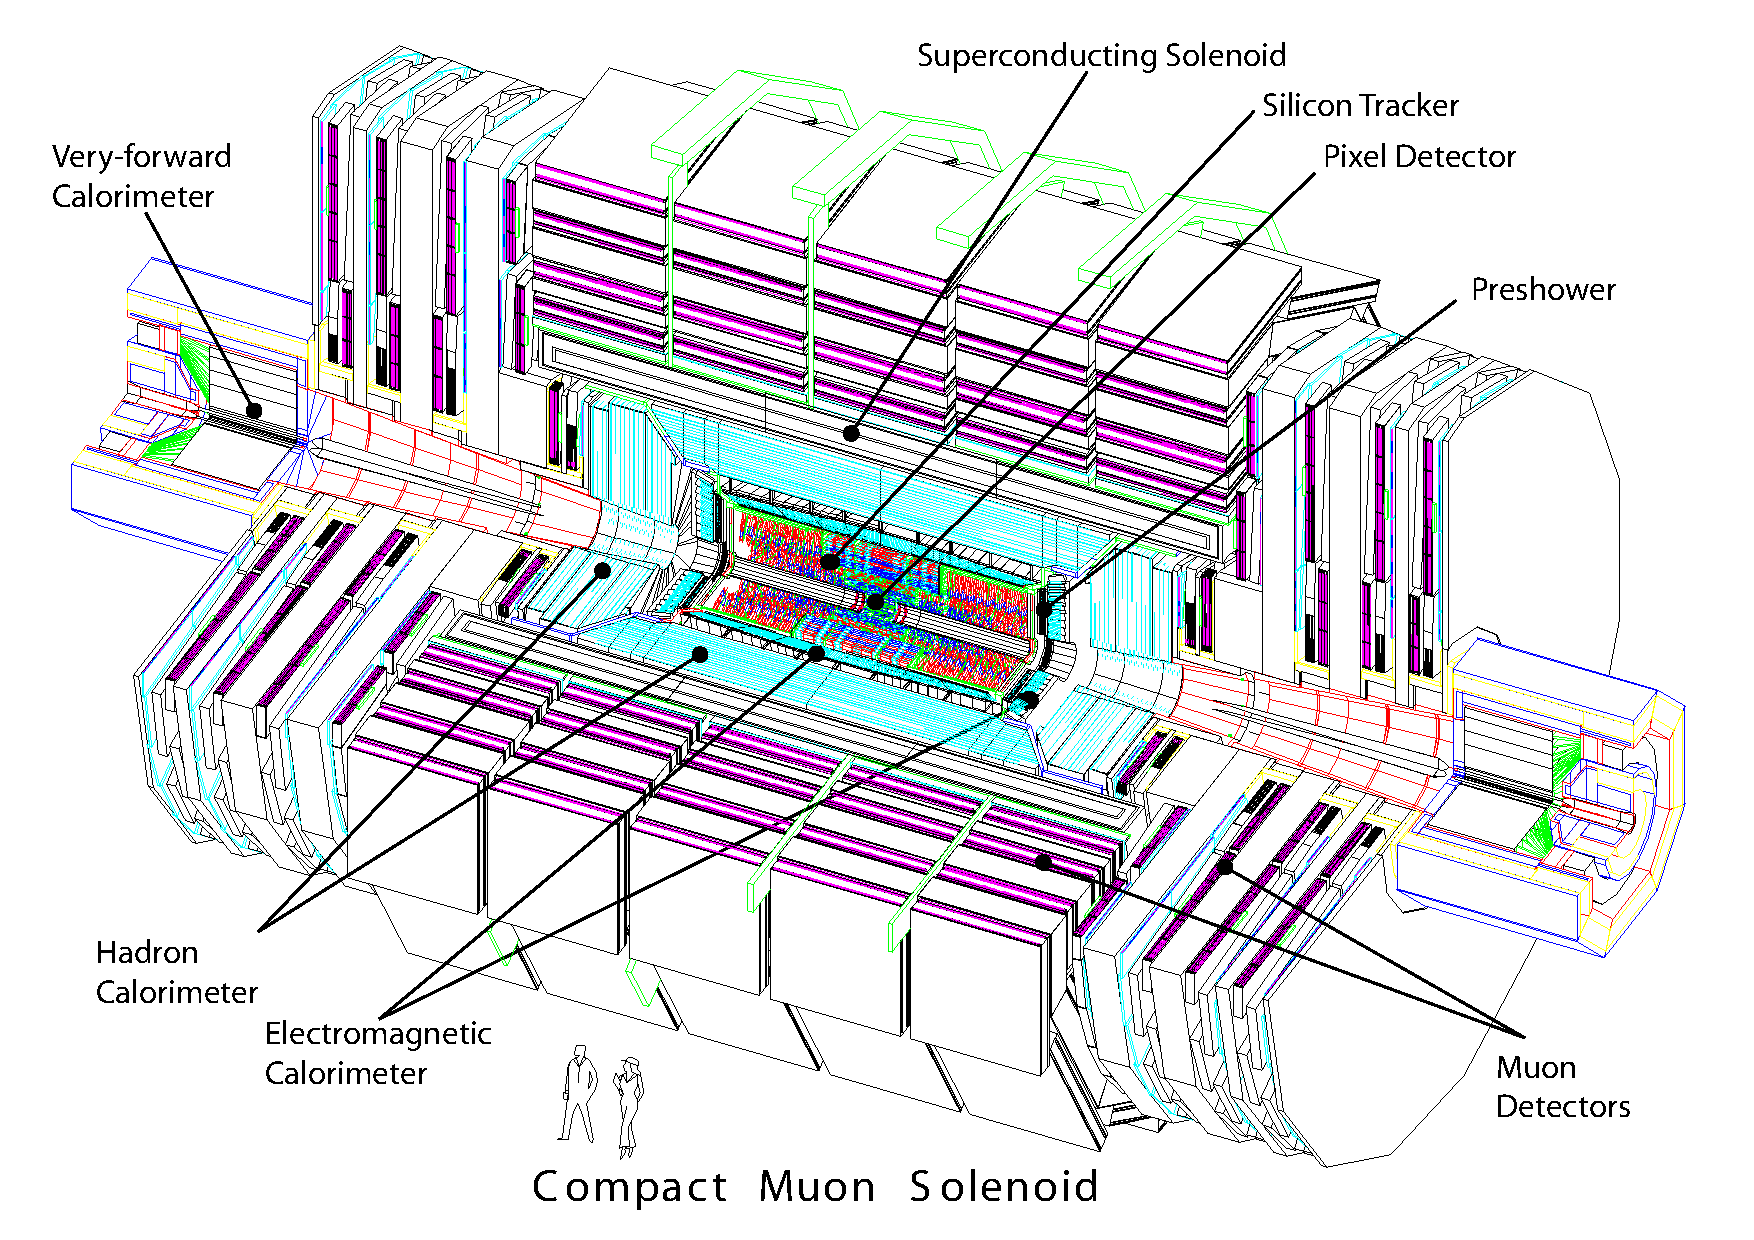
\includegraphics[width=0.95\textwidth]{cms/cms_complete_labelled}
  \caption{An exploded view of the CMS detector showing the major components.~\cite{CMS_TDR_PHYS_vol1}
  \label{fig:cms}}
\end{figure}

CMS, shown in Figure~\ref{fig:cms}, is a large and complex detector composed of multiple subsystems and detectors. Major sub-detectors include a silicon tracking detector~\cite{CMS_TRKTDR}, a crystal electromagnetic calorimeter~\cite{CMS_ECALTDR}, scintillating hadronic calorimeter~\cite{CMS_HCALTDR} and several muon detectors~\cite{CMS_MUONTDR}. The CMS detector is 21.6\,m long, has a diameter of 14.6\,m, weighs 12,500 metric tons and has $\sim\,10^{8}$ electronic readout channels. 

Charged particle momentum measurement is provided by the bending power of a 4T magnetic field. Provided by a 13 m long, 5.9 m diameter superconducting solenoid coil~\cite{CMS_MAGTDR}. The coil current is 19.5 kA giving a total stored energy of 2.7 GJ. The magnetic flux is returned by a 1.8 m thick iron return yoke. The tracking and calorimetry systems are enclosed within the coil and the return yoke is instrumented with the muon detectors.

\subsection{CMS coordinate system}
In the CMS coordinate system the origin is centred on the nominal interaction point with the x-axis pointing radially inward towards the centre of the LHC ring, the y-axis pointing vertically upward and the z-axis pointing along the beam direction towards the Jura mountains. The azimuthal angle, $\phi$, is measured from the x-axis in the x-y plane. The polar angle, $\theta$, is measured between the line connecting the coordinate to the interaction point and the z-axis. Pseudorapidity, $\eta$, is defined as $\eta=-\ln\tan(\theta/2)$. Distance in the $\phi - \eta$ plane is measured as $\mathrm{\Delta R = \sqrt{\Delta \eta^{2} + \Delta \phi^{2}}}$

Momenta and energy measured transverse to the beam, \PT and \ET respectively, are computed from their x and y components (i.e. \ET = $\mathrm{E_x + E_y}$). The energy imbalance measured in the transverse plane is denoted by \MET, where $\MET = -\ET$.

\subsection{The Silicon Tracker}

\begin{figure}[tb]
  \centering
  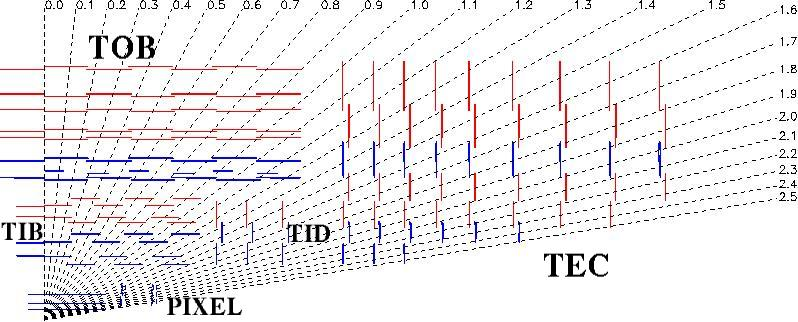
\includegraphics[width=0.95\textwidth]{cms/tk_layout}
  \caption{A one-quarter view of the tracker, showing all silicon detector layers. See the text for a description of the acronyms. Red (blue) layers use single (double) sided modules with dashed lines showing the pseudorapidity. From~\cite{CMS_TDR_PHYS_vol1}.
  \label{fig:tracker}}
\end{figure}

\begin{figure}[tb]
  \centering
  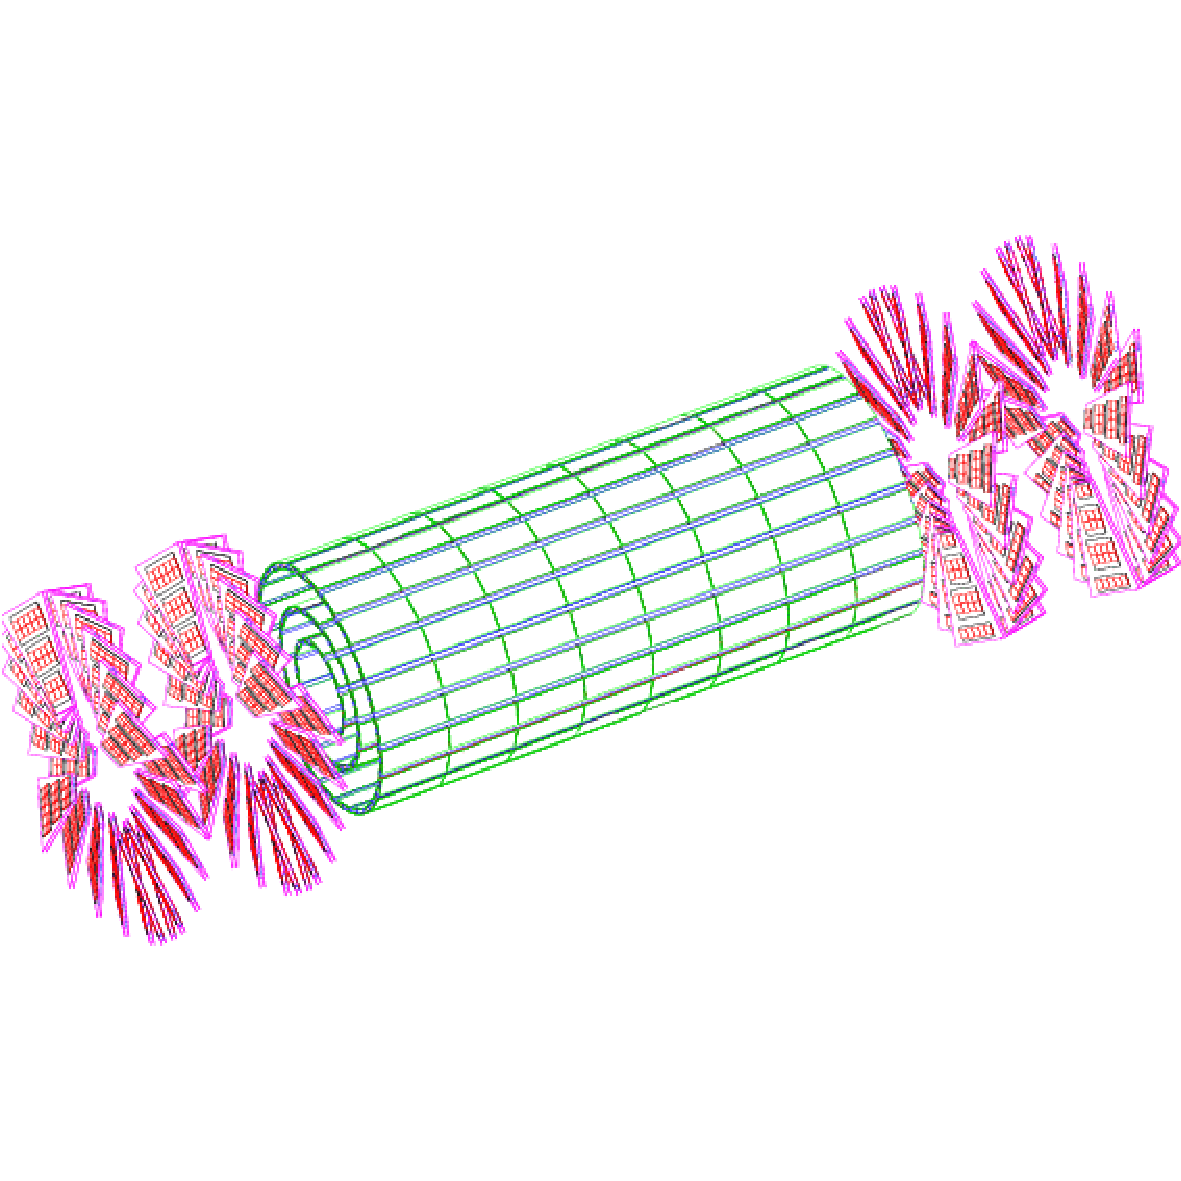
\includegraphics[width=0.8\textwidth]{cms/3l_2disk_70_0_20}
  \caption{Layout of pixel detectors in the CMS tracker.~\cite{CMS_TDR_PHYS_vol1}\label{fig:pixels}}
\end{figure}

The closest sub detector to the interaction point is the silicon tracking system. It measures the trajectories and momenta of charged particles up to $|\eta| \lesssim 2.4$. CMS has opted for a full silicon tracker providing a relatively low number of precise measurement points instead of a continuous tracking technology. Two different silicon technologies are used: pixel and microstrip detectors. Close to the beam pipe the high particle flux requires small pitch pixel detectors whereas further out the occupancy drops sufficiently to allow silicon microstrip detectors to be used. The tracker, shown in Figure~\ref{fig:tracker}, has an outer radius of 110 cm, is 540 cm long and has $\sim44\times10^{6}$ readout channels. 

The pixel detector, shown in Figure~\ref{fig:pixels}, consists of 3 barrel layers with 2 pairs of endcap disks and provides two hit coverage up to $|\eta| = 2.2$. The barrel layers are located at radii of 4.4\,cm, 7.3\,cm and 10.2\,cm and are 53\,cm long. The two endcap disks are located at $|z| = 34.5$ cm and 46.5\,cm with radii of 6\,cm to 15\,cm.

In order to maximise the vertex resolution the pixel pitch is $\approx100~\times150~\mmsquare$. The pixel spatial resolution is increased by using analogue signal interpolation of the charge sharing induced by the large Lorentz drift in the magnetic field. Thus the barrel pixel layers are collinear to the beam and the endcaps are arranged in a turbine-like geometry with blades rotated by 20\de. The spatial resolution is 10\micron in r-$\phi$ and 20\micron in z giving a vertex resolution of $\sim40\,\micron$.

The silicon strip tracker surrounds the pixel detector and covers the range $|\eta| < 2.4$. The strip tracker is split into 2 systems, inner and outer, each of which has barrel and endcap sections. Most detector layers utilise single sided microstrips but some use ``stereo'' modules consisting of two tilted back-to-back modules which provide a 3D hit measurement. The modules used in the various parts of the silicon tracker are listed in Table~\ref{tab:intro:tracker}.

\begin{table}[!h]
\centering
\begin{tabular}{lrrr}
\hline
part & No. detectors  & thickness $(\micron)$ & mean pitch $(\micron)$\\
\hline
TIB & 2724& 320 & 81/118     \\
TOB & 5208& 500 & 81/183     \\
TID & 816& 320 & 97/128/143     \\
TEC & 2512& 320 & 96/126/128/143     \\
TEC(2) & 3888& 500 &  143/158/183    \\
\hline
\end{tabular}
\caption{Detector types in the silicon tracker. See text for an explanation of the acronyms.~\cite{CMS_TDR_PHYS_vol1} \label{tab:intro:tracker}}
\end{table}

The Tracker Inner Barrel (TIB) is composed of 4 microstrip layers covering $|z| <$ 65\,cm, where the first 2 layers use stereo modules with a stereo angle of 100\,mrad. The silicon sensors have a thickness of 320\micron and a length of 10\,cm. Point resolutions of 23--34\micron in r-$\phi$ and 230\micron in z are obtained depending on the layer. Each inner endcap, Tracker Inner Disk (TID), has three microstrip layers, the first two of which have stereo modules. The microstip detectors are 320\micron thick with a minimum length of 10 cm. A point resolution of 23--34\micron in r-$\phi$ and 230\micron in z is obtained.

The outer barrel system, Tracker Outer Barrel (TOB), comprises 6 layers covering the range $|z| <$ 110 cm with the first two layers using stereo modules. The point resolution varies from 35--52\micron in r-$\phi$ and is constant at 530\micron in z. The Tracker EndCaps (TEC) comprise 9 layers over the range $120 < |z| < 280$ cm. The first two and the fifth disks have stereo modules. The microstrips have a thickness of 320--500\micron and a length of 25\,cm. A point resolution of 35--52\micron in r-$\phi$ and 530\micron in z is obtained.

%each comprised of a barrel and 2 endcap systems. The Tracker Inner Barrel (TIB) comprises 4 layers of microstrips while each endcap, Tracker Inner Disk (TID), has 3 layers

%with 2 endcap systems, Tracker Inner Disks (TID). The barrel section comprises 4 layers of microsrips while the endcaps have 3 layers. The 
%The Tracker Inner system comprises of a barrel section with 4 layers of microstrips (TIB), while the encap (TID) system includes 3 endcap disks on either side    while the encaps are ith 3 endcap disks, Tracker Inner Disks (TID), on each side. 
%microstip detectors have a minimum cell size of 10cm\times80$\mu$m and provide a point resolution of $23-34\mu m$ in r-$\phi$ and 230$\mu m$ in z. 

%The outer system 
%The Tracker Outer Barrel (TOB) comprises 6 layers with 9 endcap disks at each end. These microstrips are larger with a maximum cell size of 25cm\times180$\mu$m giving a resolution of $35-52\mu m$ in r-$\phi$ and 530$\mu m$ in z.

\begin{figure}[htb]
  \centering
  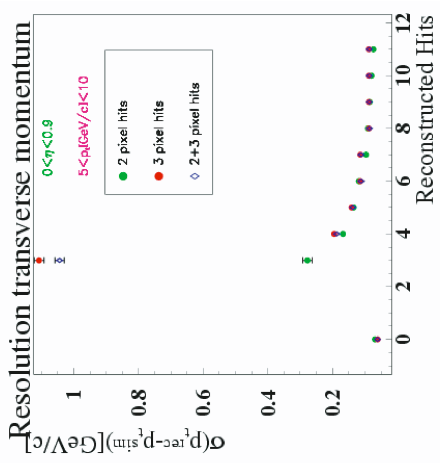
\includegraphics[width=0.45\textwidth,angle=-90]{cms/pt_perf_hits}
  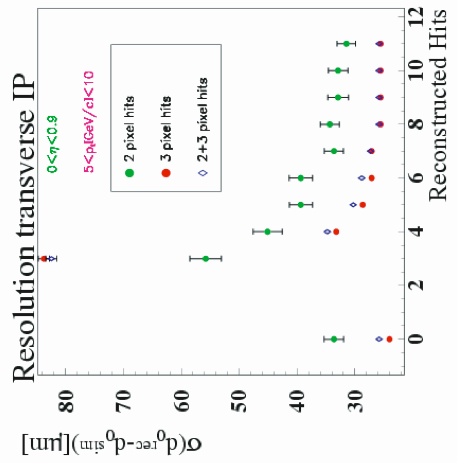
\includegraphics[width=0.45\textwidth,angle=-90]{cms/d0_perf_hits}
  \caption{The tracker \PT (left) and transverse impact parameter, d0, (right) resolution as a function of the number of reconstructed tracker hits.}
  \label{fig:tracker_perf_hits}
\end{figure}

\begin{figure}[htb]
  \centering
  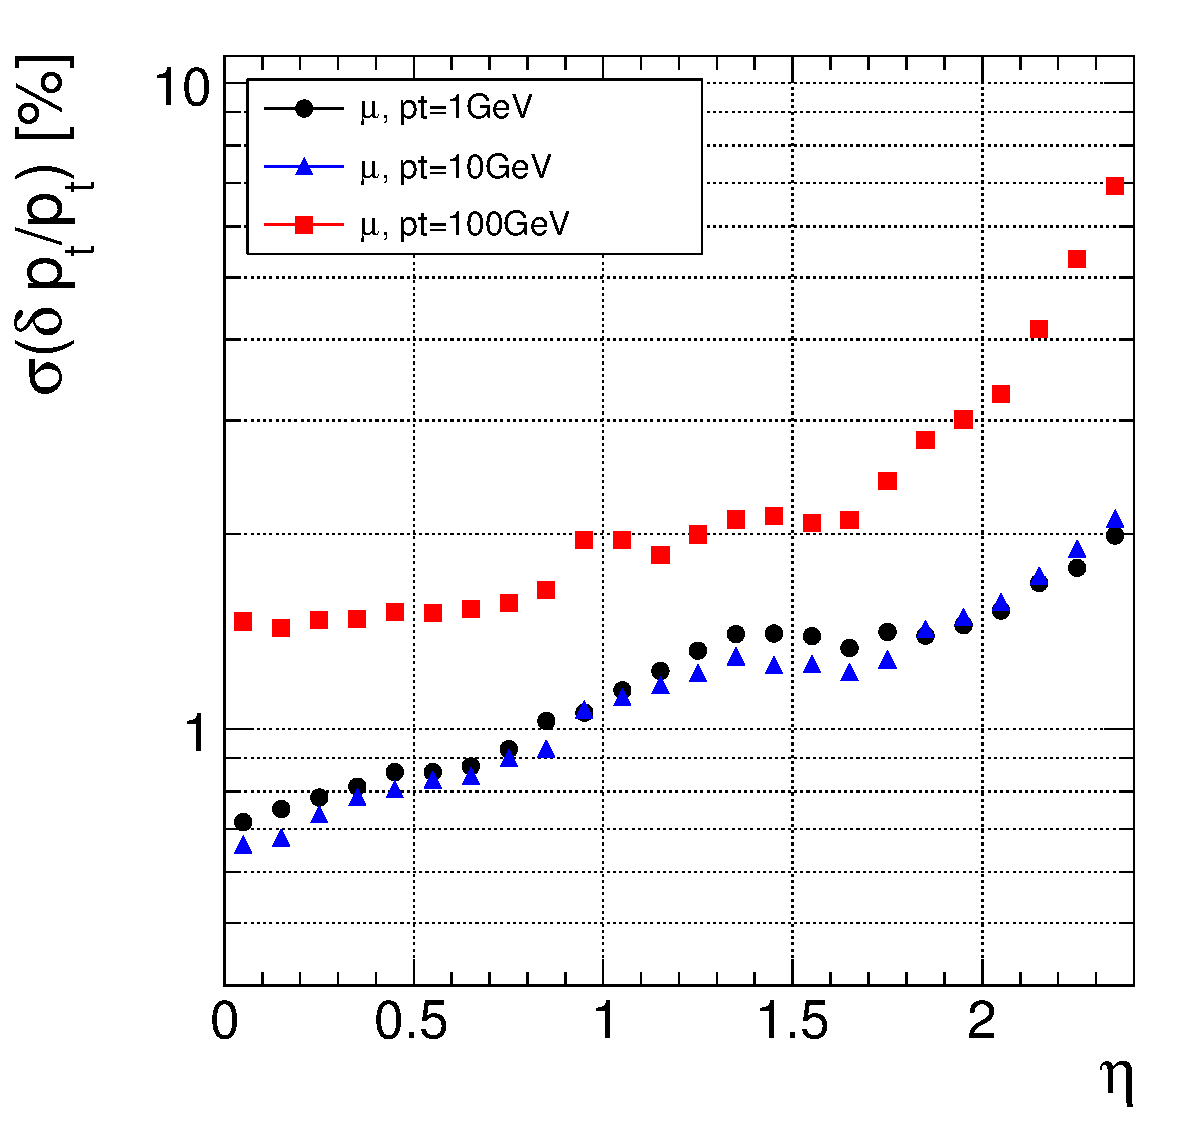
\includegraphics[width=0.45\textwidth]{cms/muon_all_pt-col}
  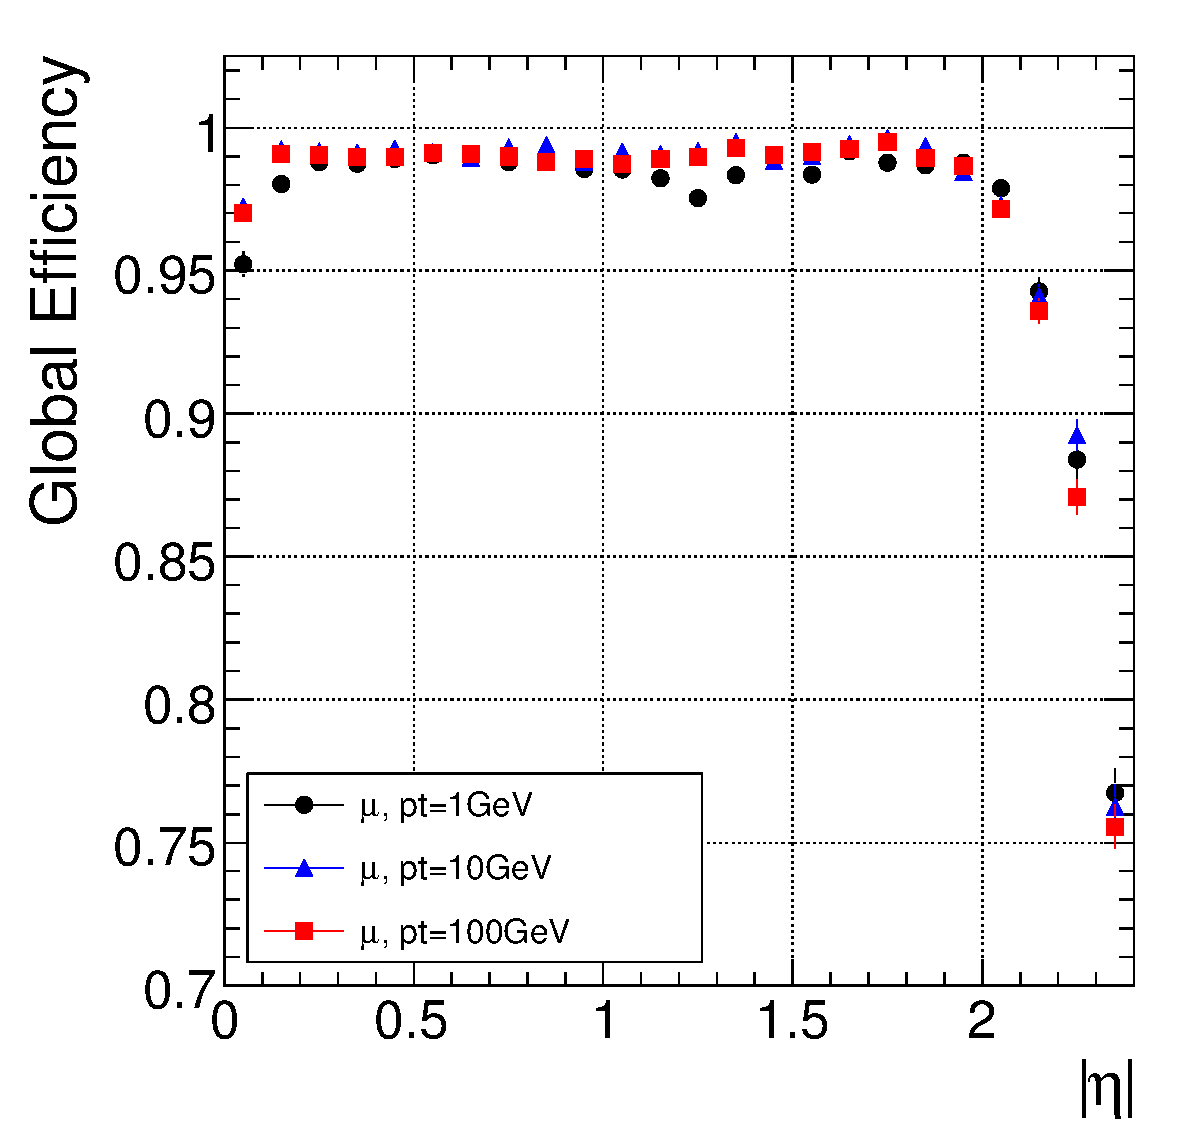
\includegraphics[width=0.45\textwidth]{cms/muonGlobalEff-col}
  \caption{Tracker performance for muons with transverse momenta of 1, 10 and 100\GeVc: transverse momentum resolution (left) and global track reconstruction
efficiency (right).~\cite{CMS_TDR_PHYS_vol1}
  \label{fig:tracker_perf}}
\end{figure}

Figure~\ref{fig:tracker_perf_hits} shows the tracker performance as a function of the number of reconstructed hits. It can be seen that performance with only the pixel layers operational is reduced. Operating in this mode is significantly quicker than using the full tracker due to the reduced number of read out channels and combinatorials and is used for triggering when less precise but fast measurements are required.

Figure~\ref{fig:tracker_perf} shows the tracker \PT resolution and global tracking efficiency for muons with \PT of 1, 10 and 100 \GeVc. Global efficiency is defined as the reconstruction efficiency for all tracks, taking into account tracker acceptance, hit efficiency and pattern recognition efficiency. The \PT resolution can be parameterised:

\begin{equation}
\frac{\sigma_{\PT}}{\PT} = a\PT \oplus 0.5\%
\label{eqn:TRK_perf}
\end{equation}

with \PT in \TeV and a = 15 for $|\eta| < 1.6$ and 60 for $1.6 < |\eta| < 2.5$~\cite{CMS_TDR_PHYS_vol1}.

\subsection{The Electromagnetic Calorimeter}
Surrounding the silicon tracker is the electromagnetic calorimeter (ECAL). The ECAL is divided into a barrel and 2 endcap sections, shown in Figure~\ref{fig:ECAL}. CMS has chosen scintillating lead tungstate (PbW$\mathrm{O_{4}}$) crystal to provide precise electron and photon energy measurement. Lead tungstate crystals are radiation hard, have short radiation lengths ($X_{0}=0.89$ cm) and are fast (80\% of light is emitted within 25 ns). This choice allowed a fast, fine grained and compact ECAL which could be placed inside the coil. PbW$O_{4}$ crystals yield a relatively low number of photons (30$\gamma$/\MeV) and so need to be read out by  photodetectors with an intrinsic gain as photo multipliers cannot operate in the high magnetic field.

\begin{figure}[htb]
  \centering
  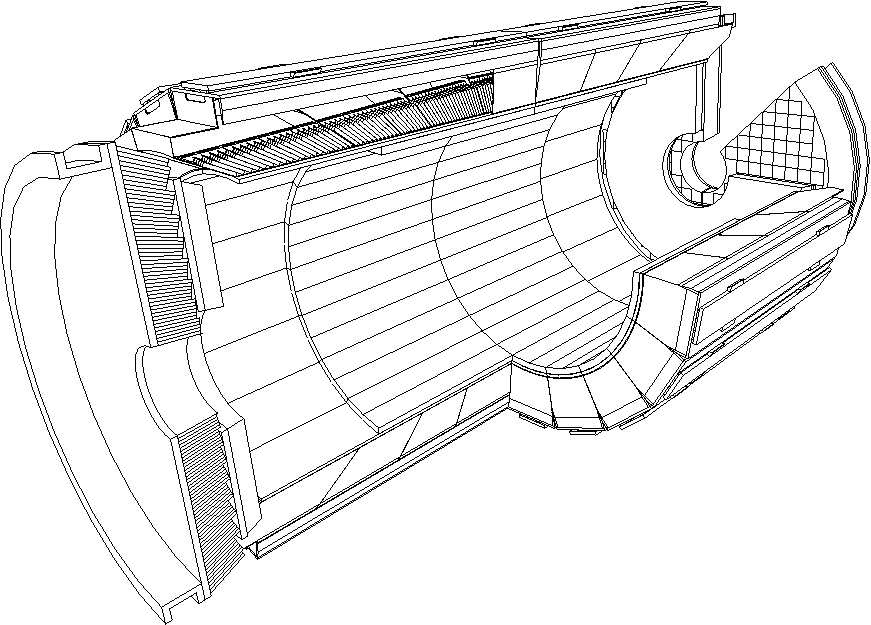
\includegraphics[width=0.85\textwidth]{cms/ECAL}
  \caption{A 3D view of the CMS electromagnetic calorimeter.~\cite{CMS_ECALTDR}}
  \label{fig:ECAL}
\end{figure}

The ECAL barrel (EB) begins at a radius of 129\,cm and covers the range $|\eta| < 1.479$. 61,200 crystals are grouped together to form one of 36 identical ``supermodules''. Each supermodule covers half of the barrel length. The crystals are mounted 3\de off axis from the nominal vertex position to avoid energy leakage between crystals. Each crystal measures $22~\times22~\times230\,\mmtriple$ (25.8 $X_{0}$) and covers an area of $\Delta\eta\times\Delta\phi = 0.0174\times0.0174$. These crystals are read out by silicon avalanche photodiodes (APDs) with a gain of 50. 

The ECAL endcaps (EE) are located 314\,cm from the vertex and cover the range $1.479 < |\eta| < 3.0$. Each endcap is constructed from two ``Dees'' consisting of semi-circular aluminium plates mounting crystals in groups of $5\times5$ crystals, known as ``supercrystals''. The endcaps crystals are tilted off axis in an x-y grid. A total of 21,528 crystals of dimensions $28.6\times28.6\times220~\mmtriple$ (24.7 $X_{0}$) are used in the endcaps. Vacuum phototriodes are used for the endcap readout as they are more radiation hard than APDs.

A preshower detector comprised of two planes of lead absorber followed by silicon strip detectors is placed in front of the endcaps, covering $1.48 < |\eta| < 2.6$. These are used to help identify neutral pions in the endcap region where the average pion energy is high enough to make resolving individual photons difficult given the calorimeter granularity.

The ECAL performance has been evaluated in a test beam~\cite{CMS_TDR_PHYS_vol1}. High energy electrons ($20 \le \ET \le 250 \GeV$) were used with a full barrel supermodule. The measured electron energy resolution is shown in Figure~\ref{fig:ECAL_perf}. The resolution can be parameterised as 

\begin{equation}
	\frac{\sigma}{E} = \frac{3.63\%}{\sqrt{E}} \oplus \frac{0.124\%}{E} \oplus 0.26\%,
\label{eqn:ECAL_perf}
\end{equation}

where E is the beam energy in \GeV, the first term is the stochastic term, the second the noise and the third the constant term. The Stochastic term comes from fluctuations in lateral containment and photostatistics~\cite{CMS_TDR_PHYS_vol1}, the noise term originates from preamplifier, digitisation and pileup noise, and the constant term comes from energy leakage and inter-crystal calibration.

\begin{figure}[tb]
  \centering
  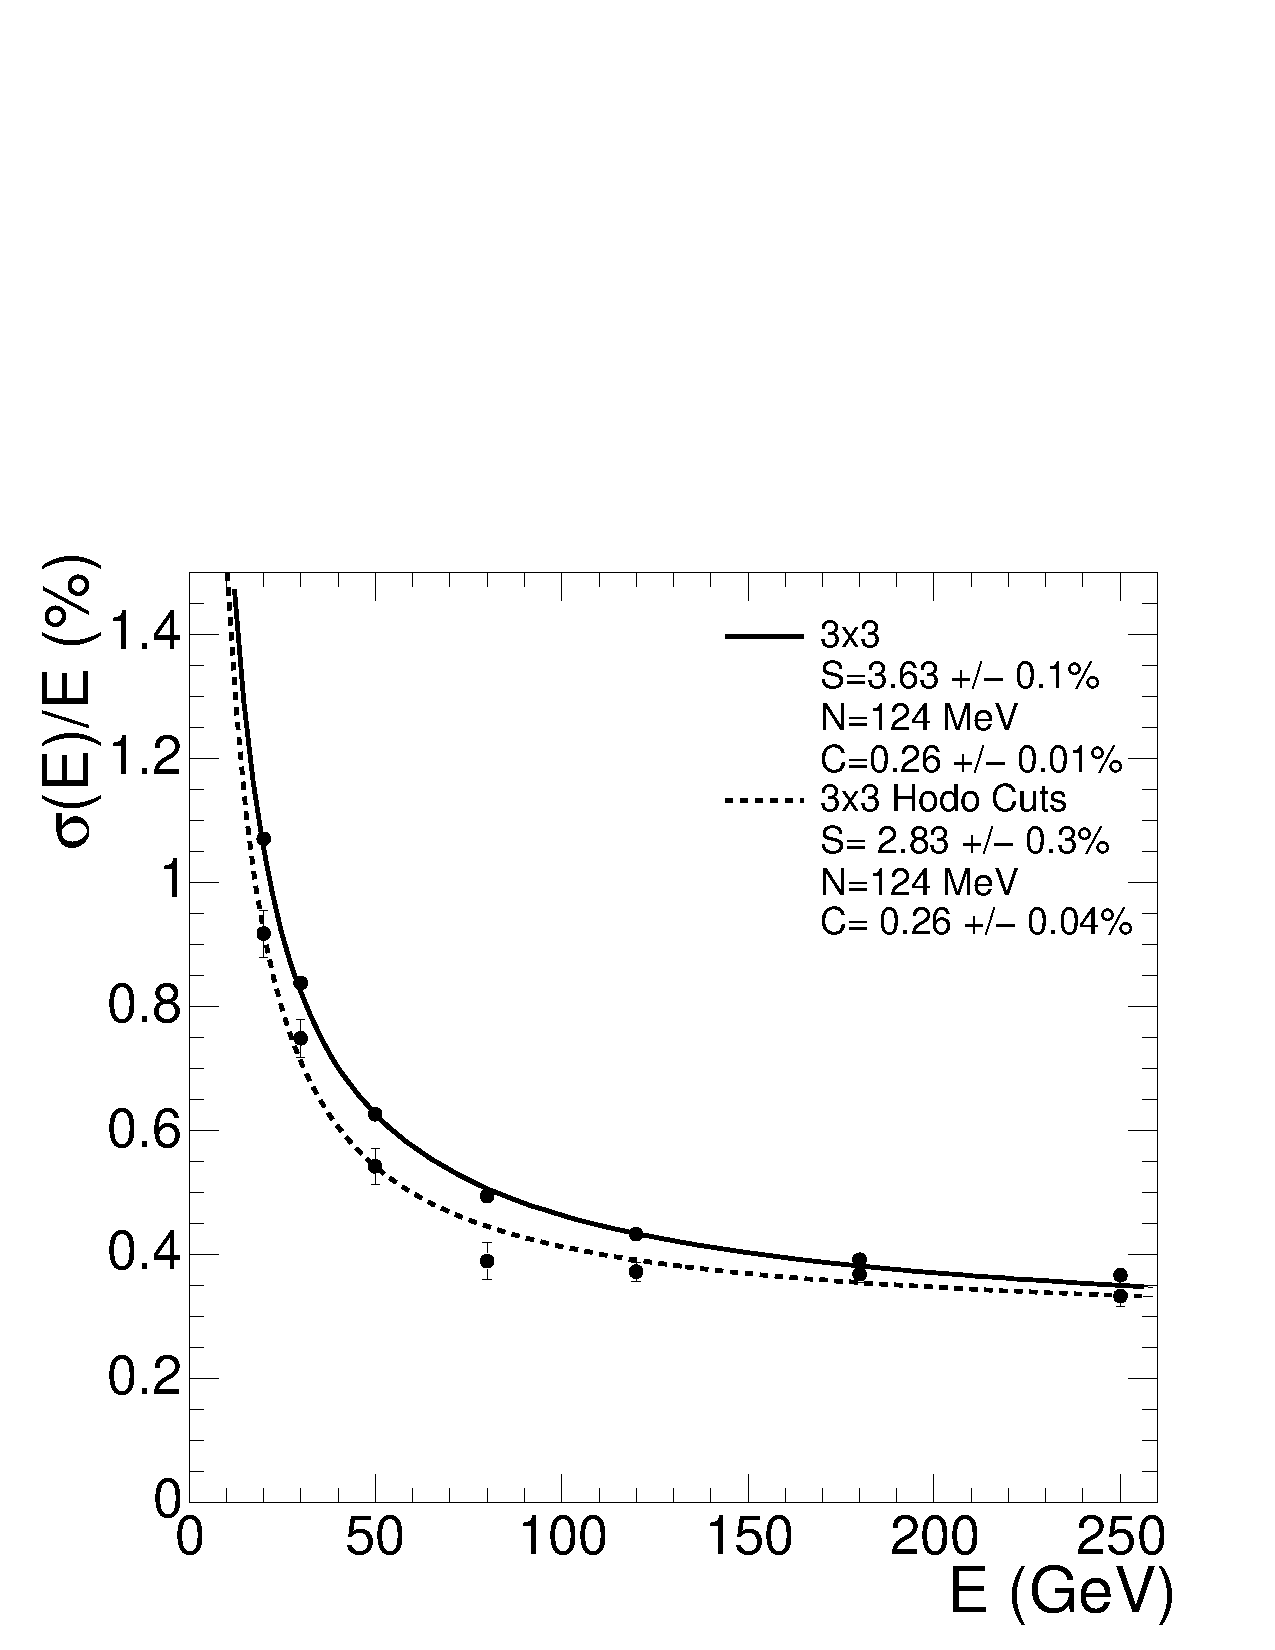
\includegraphics[width=0.55\textwidth]{cms/Resolution_Comp_Hodo_3x3_704_tdr}
  \caption{ECAL electron test beam data energy resolution as measured by an array of 3$\times$3 crystals. The upper (lower) series shows events taken with a 20$\times$20 (4$\times$4)\,~\mmsquare trigger. The fit parameters correspond to those in Equation~\ref{eqn:ECAL_perf}.~\cite{CMS_TDR_PHYS_vol1}
  \label{fig:ECAL_perf}}
\end{figure}


%%%%%
%These are used for neutral pion rejection by resolving the individual photons in the decay. A preshower is not needed for the barrel as the average pion energy in this region is low resulting in a large opening angle between the two photons. Which together with the granularity of the crystal detector alow both to be resolved.
%%%%%

\subsection{The Hadronic Calorimeter}
Surrounding the electromagnetic calorimeter is the hadronic calorimeter (HCAL). In order to minimise non-Gaussian energy resolution tails and to provide good containment the HCAL was placed inside the magnet coil. This required a compact absorber and left little room for the active medium. Brass was chosen for the absorber because it is non-magnetic and has a short interaction length ($\lambda$). Tile/fibre technology was chosen for the active medium together with wavelength-shifting fibre readouts. 

The barrel section, denoted HB, spans the region $|\eta| < 1.4$ and is read out in towers of $\Delta\eta \times \Delta\phi = 0.087\times0.087$ in a single longitudinal sampling. The HB has 15 brass plates comprising 6.5\,$\lambda$ thus additional layers, known as the hadron outer (HO), are placed behind the coil, hadron outer (HO), to act as a tail catcher. This covers the region $|\eta| < 1.26$ and uses the same tower geometry as the barrel. The HO extends the barrel HCAL depth to over 10\,$\lambda$.
 
Hadron endcap (HE) disks are located either side of the solenoid coil and span the region $1.3 < |\eta| < 3.0$ with towers varying in size from $\Delta\eta \times \Delta\phi = 0.087\times0.8 - 0.35\times0.8$.

To extend the $\eta$ coverage, a forward calorimeter, hadron forward (HF), is located at the edges of CMS covering the region $3.0 < |\eta| < 5.0$ (see Figure~\ref{fig:cms}). This detector is constructed from steel and quartz fibre. These materials lead to shorter and narrower jets which is useful in the high flux forward region.

\begin{figure}[tb]
  \centering
    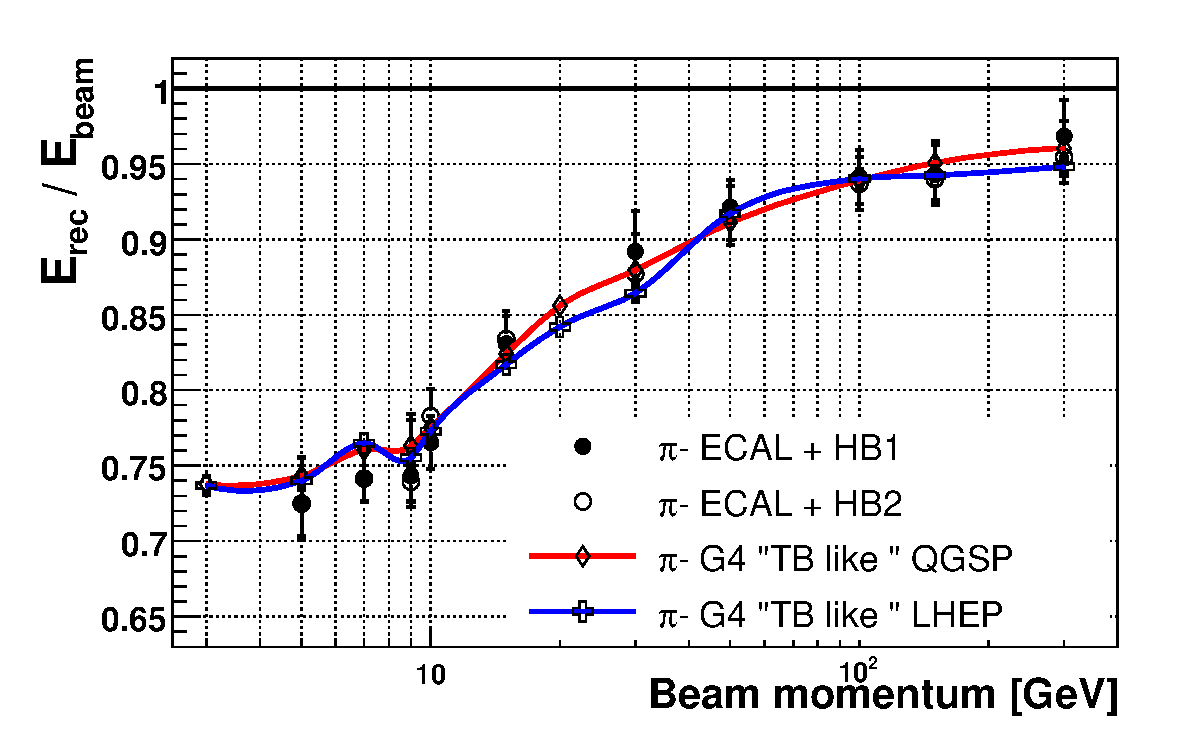
\includegraphics[width=0.48\textwidth]{cms/linearity5-300}
    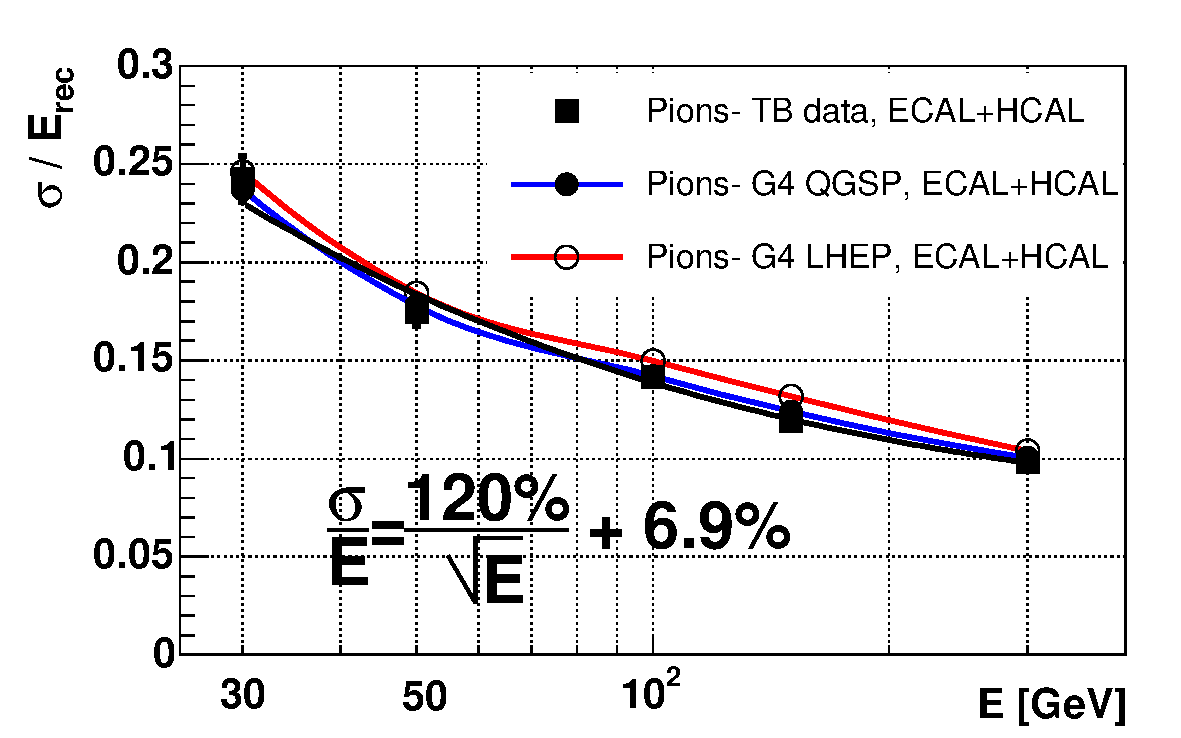
\includegraphics[width=0.48\textwidth]{cms/res_fit}
    \caption{Nominal raw energy response and fractional energy resolution 
as a function of ECAL+HB energy for \piminus. The fit for the non-compensated
energy resolution is shown. Results for both testbeam and simulated (labeled G4) data are shown.~\cite{CMS_TDR_PHYS_vol1}}
    \label{fig:HCALparticle}
\end{figure}

Test beams have been used to evaluate the HCAL performance and characteristics. The 2004 HCAL test beam used a replica of a slice through the CMS detector with a \piminus beam~\cite{CMS_TDR_PHYS_vol1}. The prototype detector included an aluminium slab, representing the solenoid, a prototype ECAL detector and 144 HB and 60 HO towers. This detector was exposed to \piminus beams of energies 2-9~\GeV and 10-300~\GeV. The single particle energy response and resolution are shown in Figure~\ref{fig:HCALparticle} both for test beam and simulated data. The energy resolution can be parameterized as:

\begin{equation}
	\frac{\sigma}{E}= \frac{120\%}{\sqrt{E}} \oplus 6.9\%
\end{equation}

The HCAL jet and \MET performance have been evaluated with simulated QCD multi-jet events at \lowlumi~\cite{CMS_TDR_PHYS_vol1}. The jet energy response for jets of various generated \ET (\ETMC) is shown in Figure~\ref{fig:jet_scale}.

\begin{figure}[bt]
   \centering
    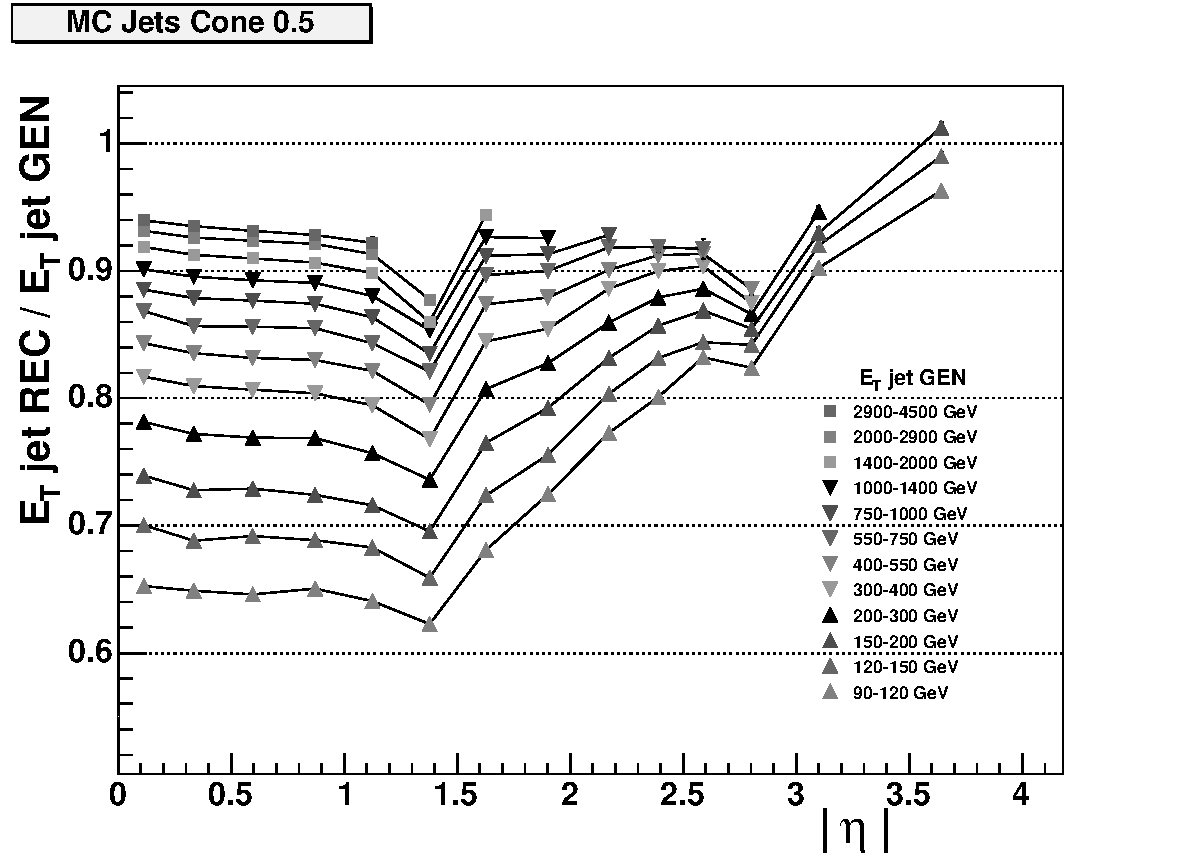
\includegraphics[width=0.8\textwidth]{cms/EtaG_grey}
    \caption{The ratio of the reconstructed jet transverse energy $\mathrm{E_{T}^{rec}}$ 
      to the generated transverse energy \ETMC
      as a function of generated jet $\eta$ for jets with
      different \ETMC reconstructed by the iterative cone
      $R=0.5$ algorithm.~\cite{CMS_TDR_PHYS_vol1}}
    \label{fig:jet_scale}
\end{figure}

\begin{figure}[hbt]
  \centering
  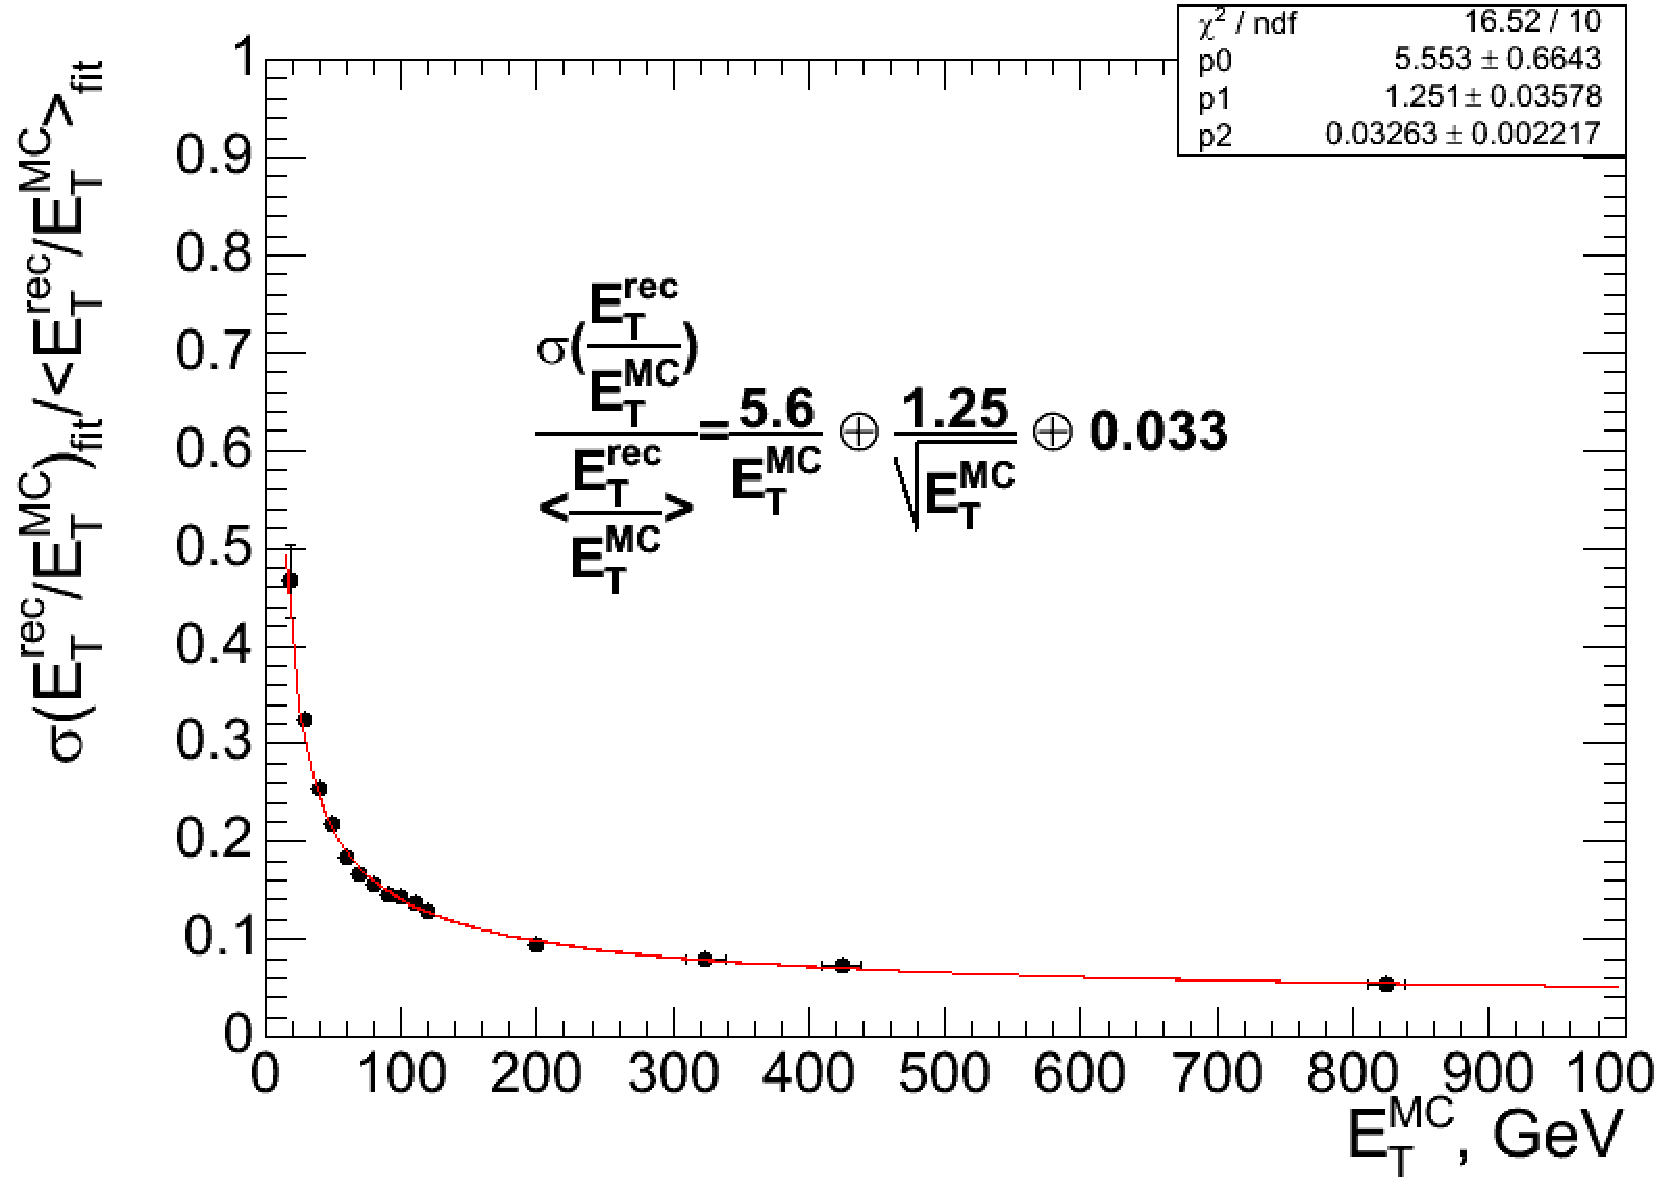
\includegraphics[width=0.8\textwidth]{cms/et_resolution_0508_dr02_bar_cor}
  \caption{The jet transverse energy resolution for simulated jet events with pileup in the HCAL barrel.~\cite{CMS_TDR_PHYS_vol1}
  \label{fig:Jet_perf}}
\end{figure}

The granularity of the different HCAL detectors has been chosen to provide similar jet energy resolutions for all regions. The barrel jet energy resolution can be seen in Figure~\ref{fig:Jet_perf} and can be parameterised: 

\begin{equation}
\mathrm{\frac{\sigma\left(\frac{E_{\rm T}^{\rm rec}}{E_{\rm T}^{\rm MC}}\right)}{\langle\frac{E_{\rm
      T}^{\rm rec}}{E_{\rm T}^{\rm MC}}\rangle}=\frac{5.6}{\ETMC} \oplus
      \frac{1.25}{\ETMC} \oplus 0.033}
\end{equation}

where the first term is the noise term, the second the stochastic term and the third the constant term. The noise is due to fixed energy fluctuations from electronic noise, pileup and the underlying event, the second term is the stochastic calorimeter response and the third is a constant term originating from the non-uniformities and non-linearities of the calorimeter response.

The missing energy \MET mean and resolution distributions for soft ($0 < \PT < 15 \GeV$) QCD dijet events with pile-up are shown in Figure~\ref{fig:MET_perf}. These can be parameterised as:

\begin{equation}
 \langle\MET\rangle \approx 1.25 \sqrt{ \Sigma \ET}
 \label{eqn:MET_mean}
\end{equation}

and

\begin{equation}
 \sigma(\MET)\approx 1.0 \sqrt{ \Sigma \ET}
 \label{eqn:MET_SIGMA}
\end{equation}

\begin{figure}[bt]
  \centering
  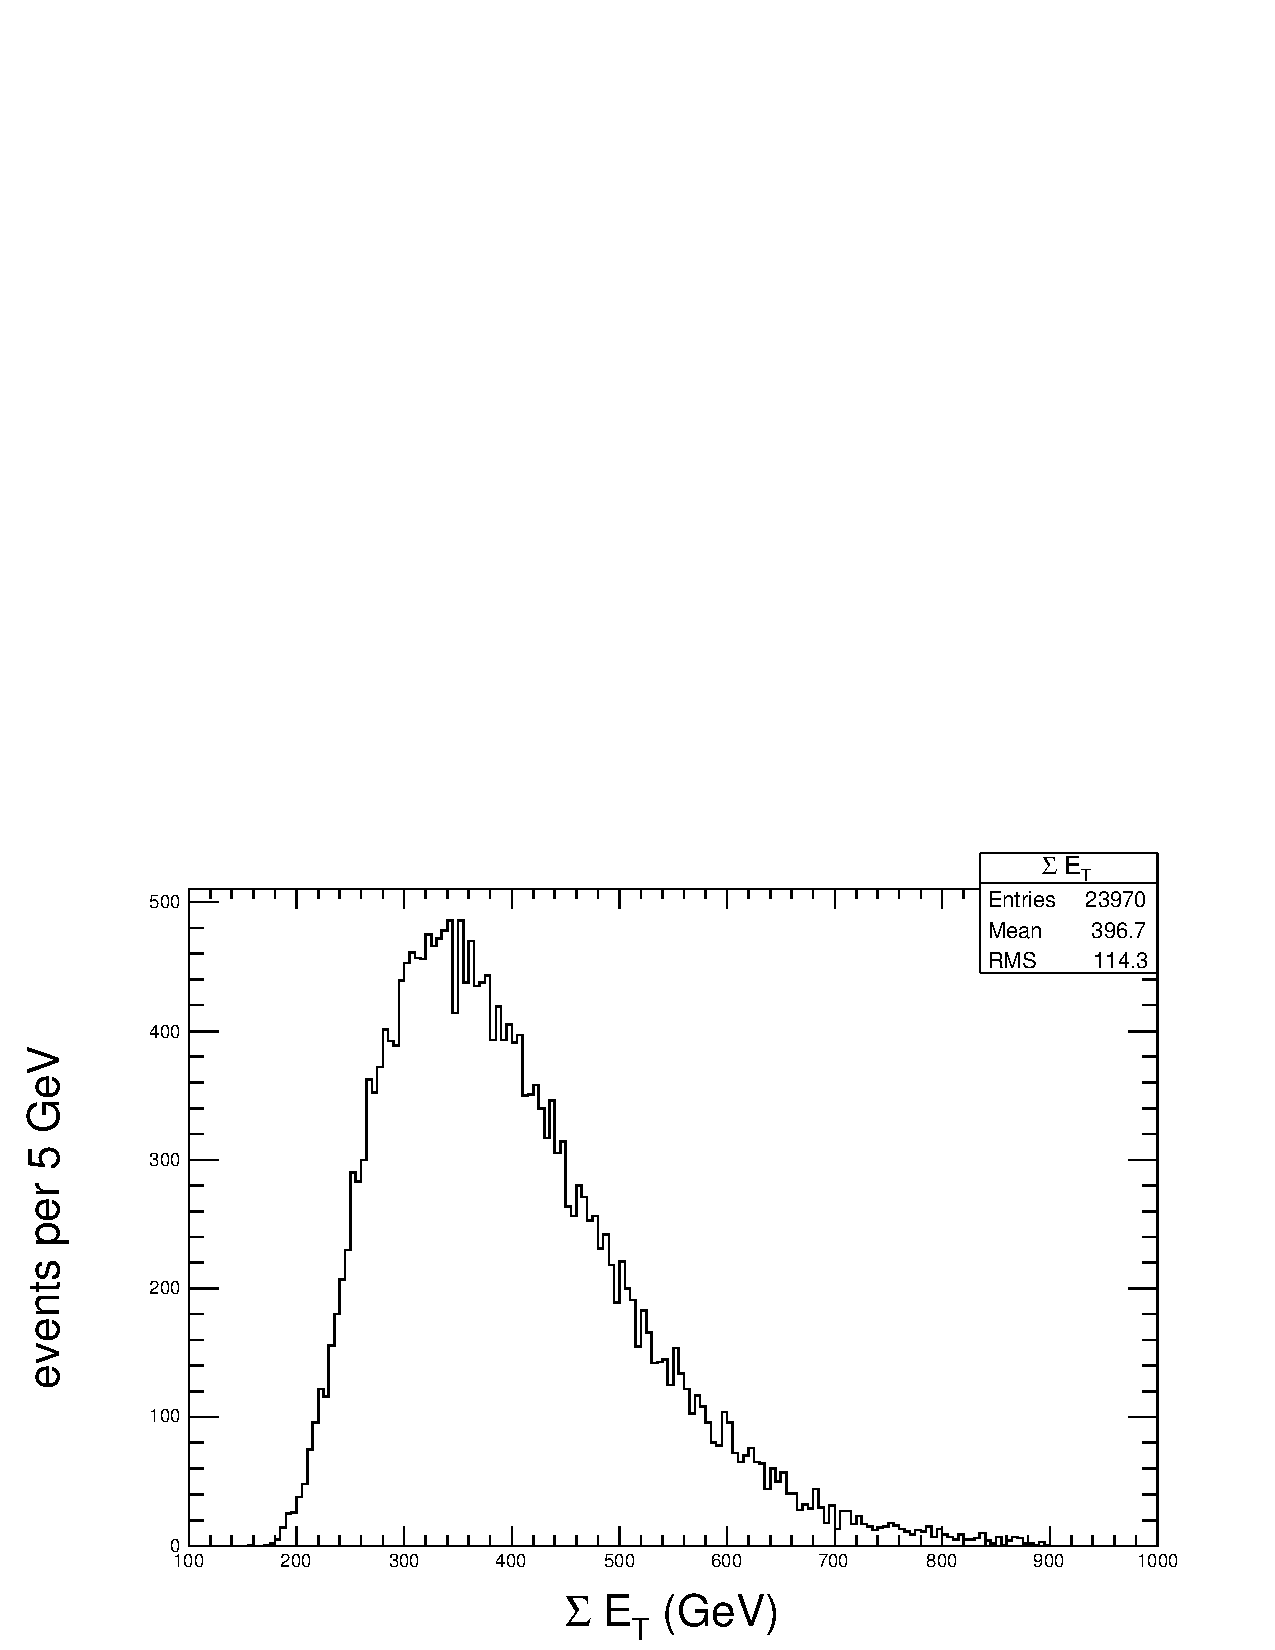
\includegraphics[width=0.45\textwidth]{cms/QCD-0-15-SumEt}
  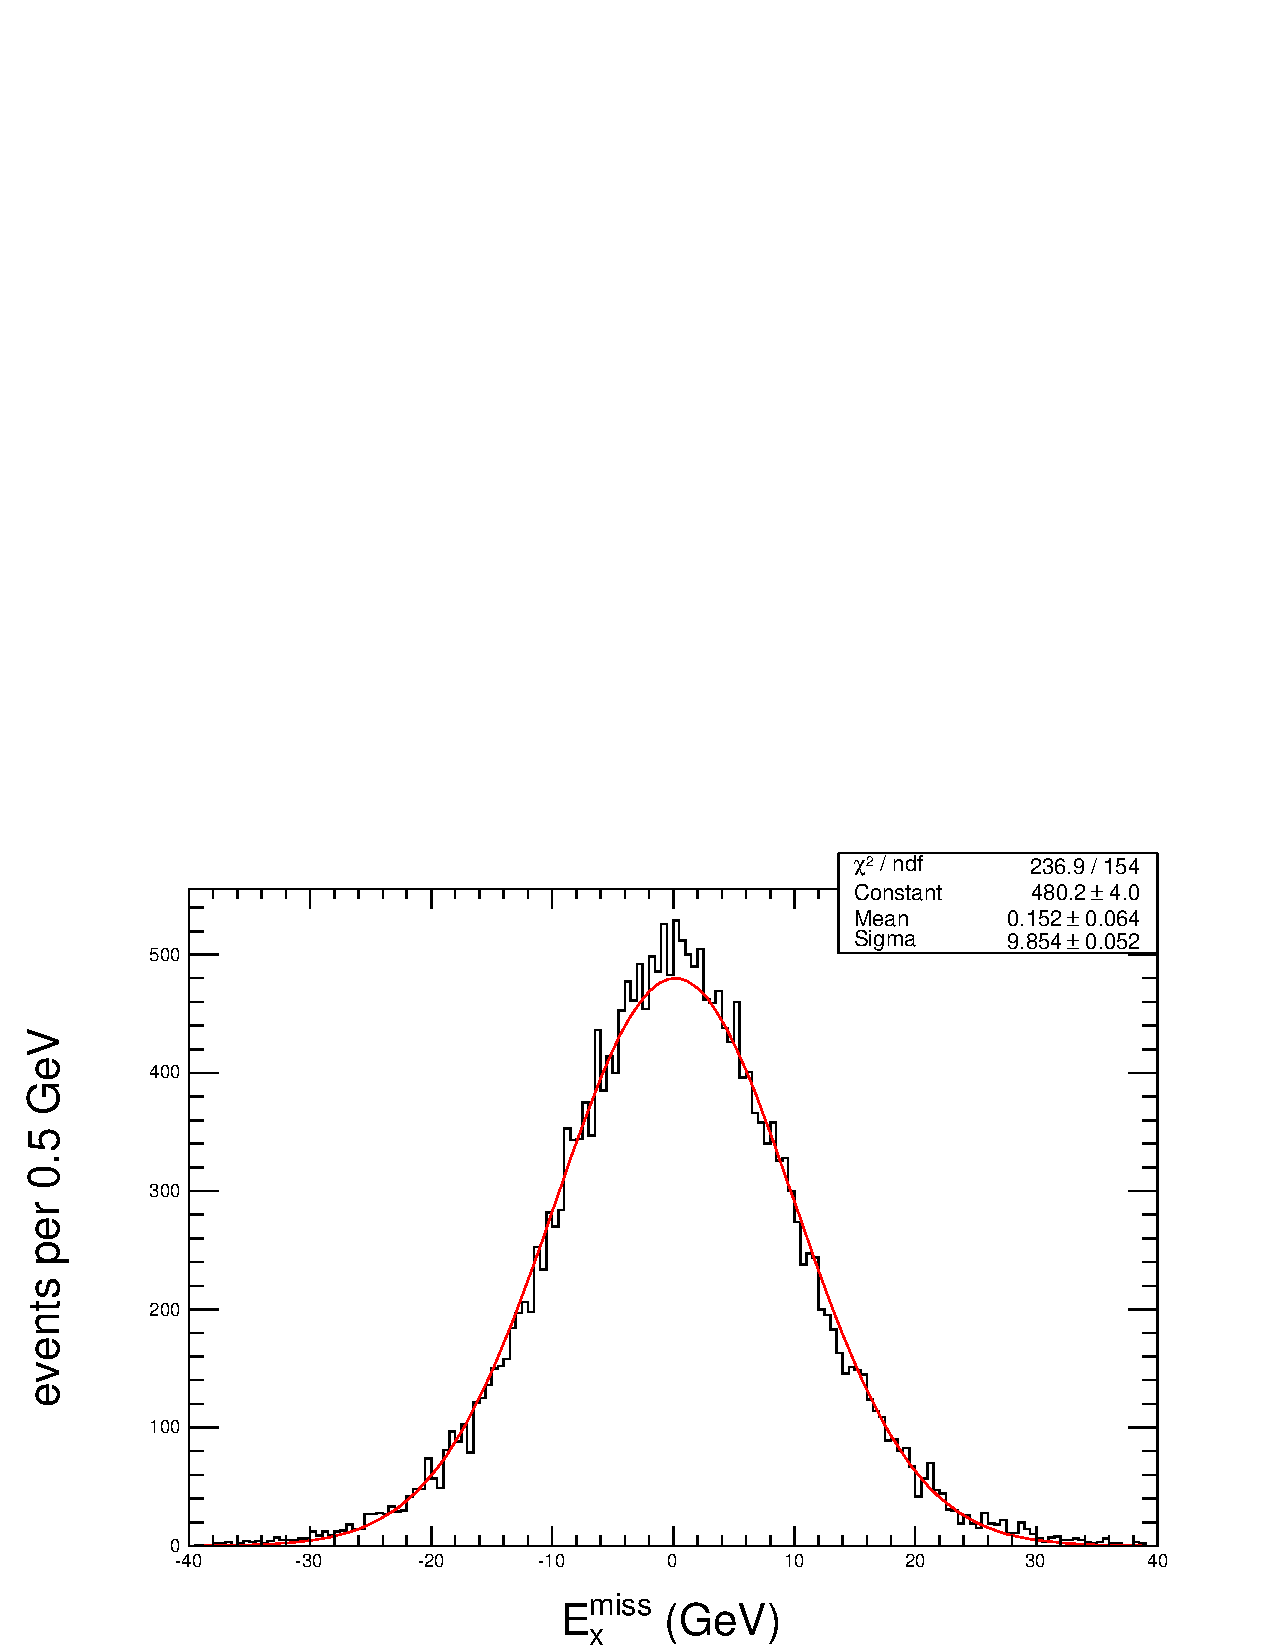
\includegraphics[width=0.45\textwidth]{cms/QCD-0-15-METx}
  \caption{Distribution of sum \ET (left) and $\mathrm{E_{x}^{miss}}$ (right) for soft QCD events with pileup. The \MET resolution of 9.9GeV is in good agreement with Equation~\ref{eqn:MET_SIGMA}.~\cite{CMS_TDR_PHYS_vol1}
  \label{fig:MET_perf}}
\end{figure}

\subsection{The Muon Detectors}
The Muon system provides measurements in the range $|\eta| < 2.4$ and is shown in Figure~\ref{fig:muons}. Detectors are placed at four layers or stations in the barrel and endcap sections of the iron flux return. Three different types of gaseous detector are used due to the varying radiation and magnetic environments. The barrel section, covering $|\eta| < 1.2$, uses drift tubes (DT). The high muon and neutron background environment of the endcaps, $0.8 < |\eta| < 2.4$, means cathode strip chambers (CSC) are used instead of DTs. Resistive Plate Chambers (RPC) are used in both the barrel and part of the endcaps, $|\eta| < 2.1$.

The barrel region contains 250 chambers of up to 12 planes of drift tubes. The individual drift tubes have a cross section of $42 \times 13\,\mmsquare$ and are filled with Ar and $\mathrm{CO_{2}}$. Each drift tube consists of a central anode wire surrounded by aluminum cathodes. The induced charge has a maximum drift length of 2 cm or 400 ns. Each station provides a muon vector with a resolution of 100\micron in $\phi$ and 1 mrad in direction.

The two endcaps use 468 CSCs each of which is trapezoidal and contains 6 gas gaps. Each gap has a plane of radial cathode strips with perpendicular anode wires. The muon position is measured from the charge sharing of the radial cathode strips. Each station provides a muon vector with a resolution of $\sim$200\micron in $\phi$ and 10\,mrad in direction. 

The RPCs consist of a gas gap enclosed by two graphite-coated bakelite plates. The graphite forms a cathode with an aluminum strip used to read out the generated signal. The RPCs have a time resolution of $\sim$1\,ns which makes them useful for identifying the bunch crossing time. 

\begin{figure}[htb]
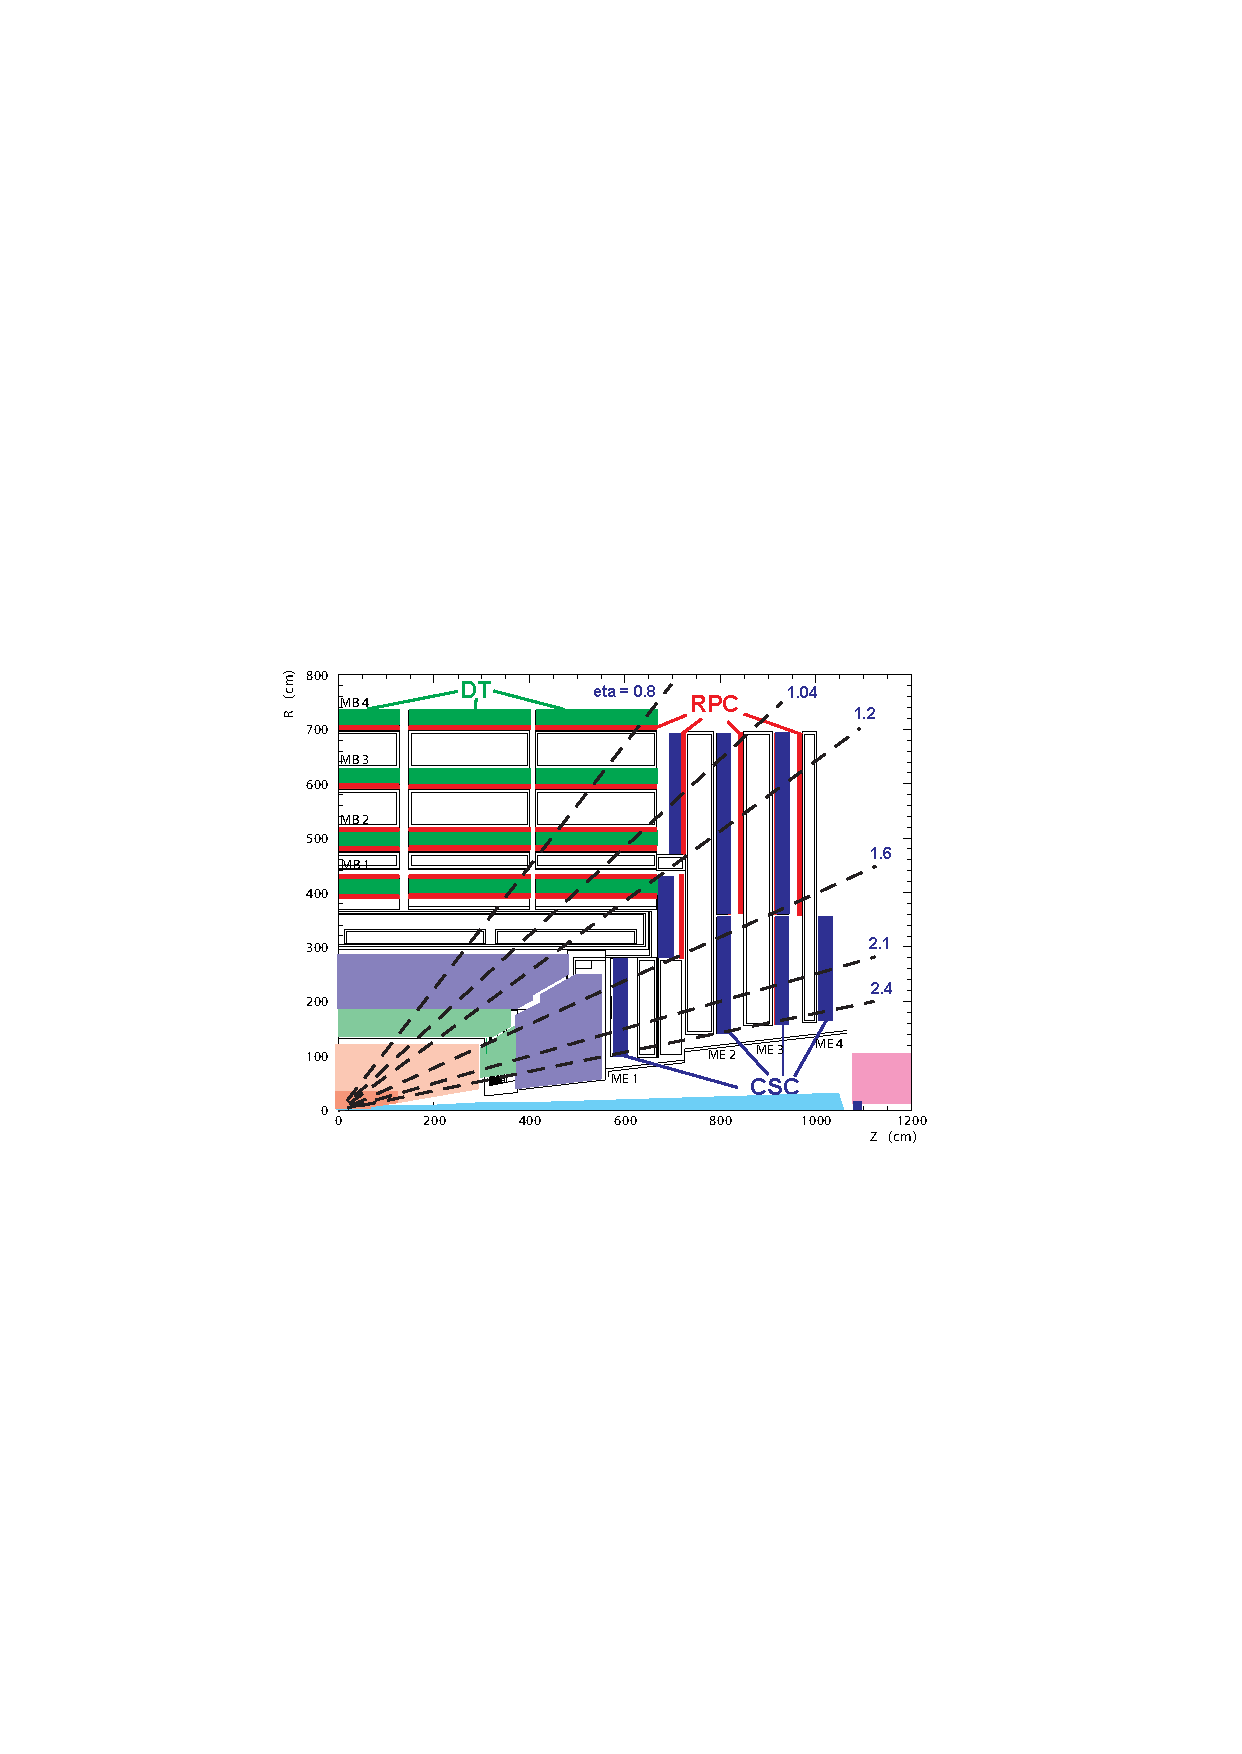
\includegraphics[width=0.9\textwidth]{cms/CMSQuarterView_new}
\caption{Layout of one quarter of the CMS muon system for initial low
luminosity running. The RPC system is limited to $|\eta|<1.6$ in the endcap, and
for the CSC system only the inner ring of the ME4 chambers have been deployed.~\cite{CMS_TDR_PHYS_vol1}
\label{fig:muons}}
\end{figure}

The muon system has a tracking efficiency of over 90\% for 100\GeV muons. The resolution of the muon system, shown in Figure~\ref{fig:muonresol}, is dominated by multiple scattering from the detector materiel in front of the muon detectors. At low momenta the resolution can be improved by using information from the tracker. At higher momenta multiple scattering can be neglected. The muons are then bent in equal and opposite directions before and after the coil, and this can be used at high energies to improve the resolution.

\begin{figure}[tb]
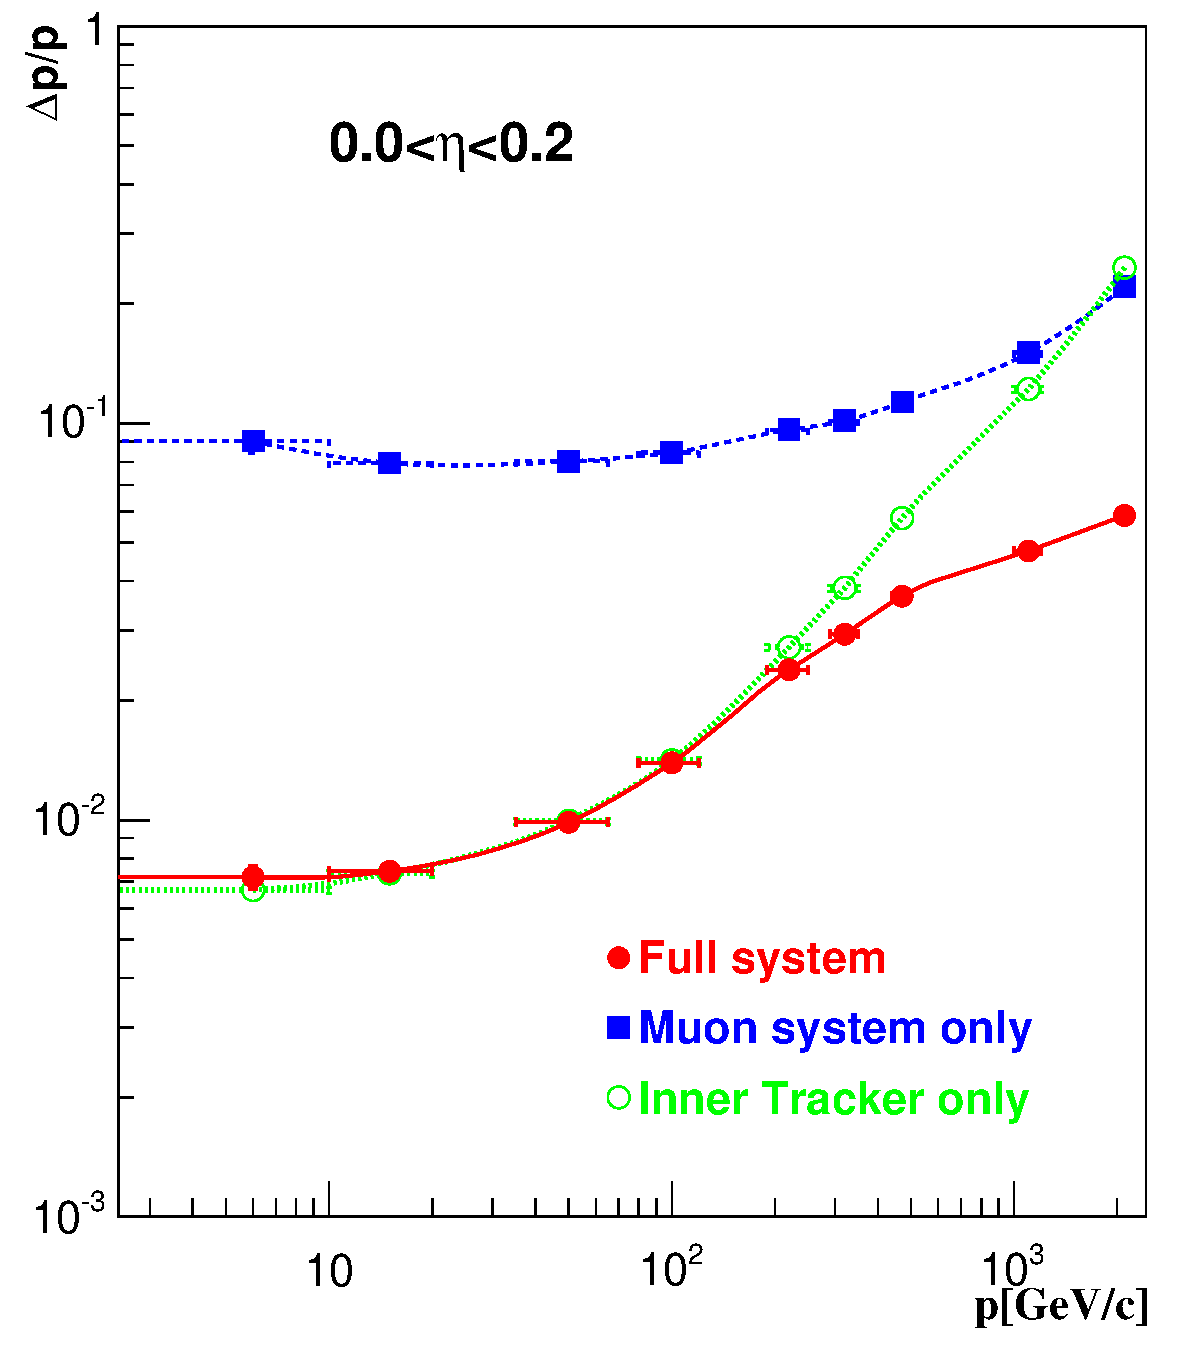
\includegraphics[width=0.48\textwidth]{cms/p_barrel}
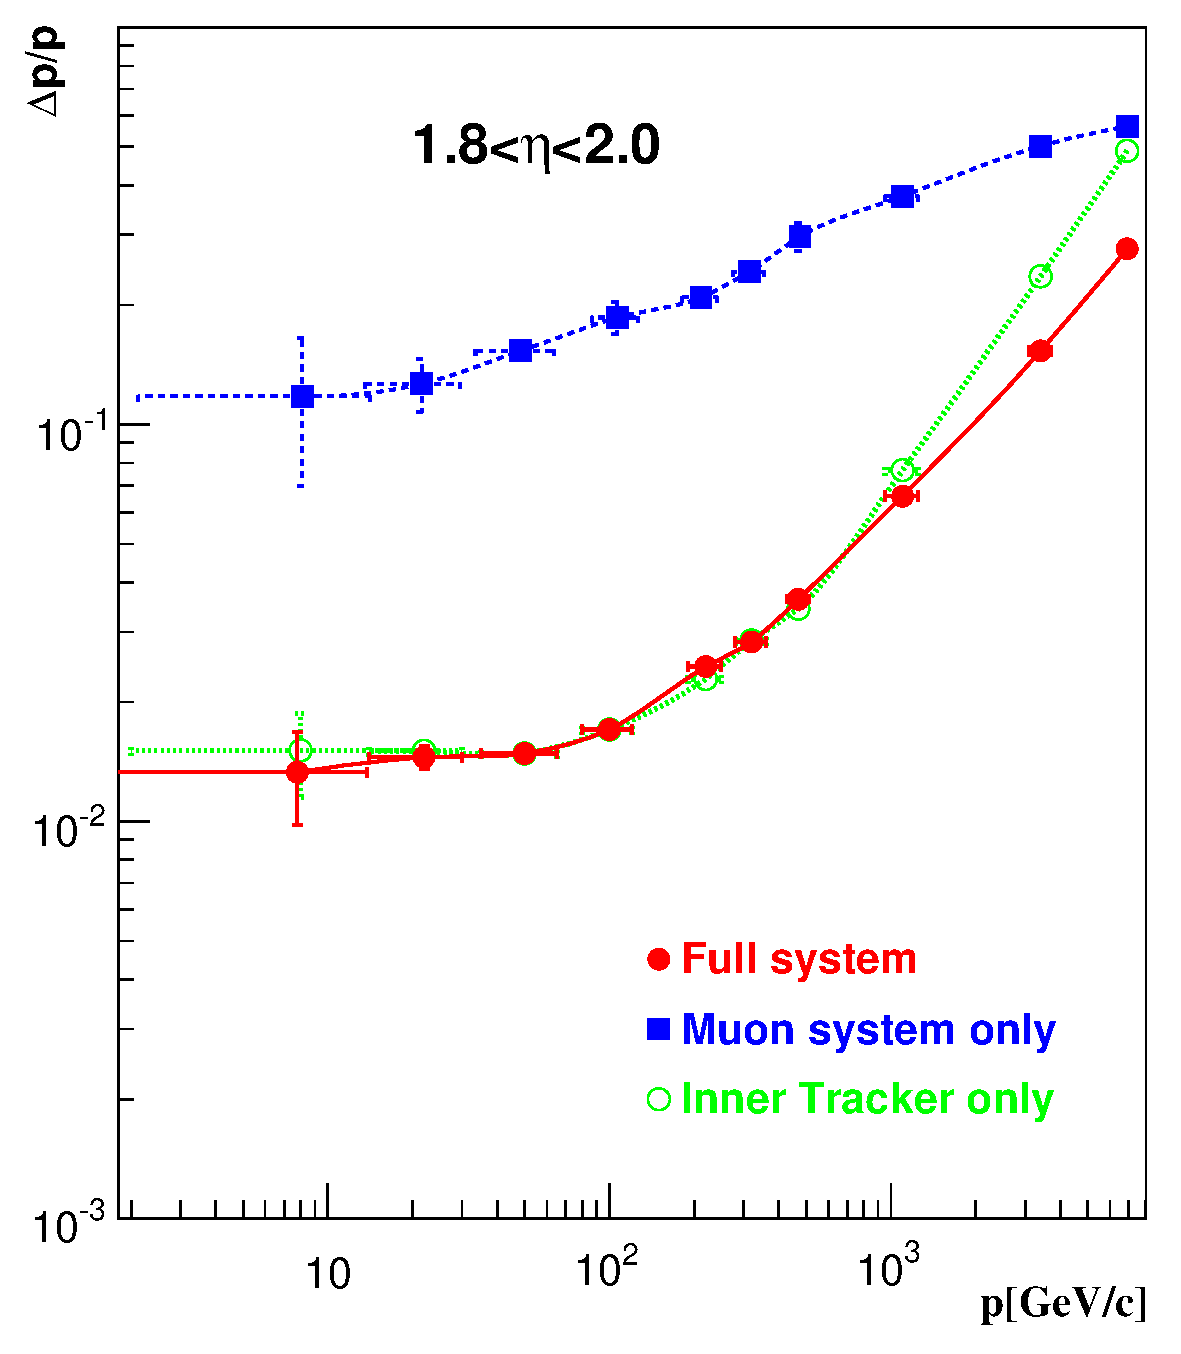
\includegraphics[width=0.48\textwidth]{cms/p_endcaps}
\caption{The muon momentum resolution versus $p$ using the muon
system only, the inner tracker only, or both (``full system''). For the  barrel, $|\eta|<0.2$ (left) and endcap, $1.8<|\eta|<2.0$ (right).~\cite{CMS_TDR_PHYS_vol1}
  \label{fig:muonresol}}
\end{figure}

\subsection{The Trigger System \label{sec:trigger}}
At $\sqrt{s} = 14\TeV$ the proton-proton inelastic cross section is roughly 100 mb. At design luminosity (\hilumi) this results in $10^{9}$ inelastic interactions/s. Given the LHC bunch crossing interval of 25ns (40 MHz), this yields an average of 20 inelastic collisions per bunch crossing (event). Given that CMS has $\sim10^{8}$ detector channels and one event comprises $\sim 1$ MB of data this would give rise to a data rate of 100 TB/s. Storage systems place a limit of 100--200 MB/s, hence an online selection (``trigger'') is used to reduce the event rate to $\sim$100 Hz. 

The CMS trigger is split into two parts; a fast hardware (Level-1) trigger and a software High Level Trigger (HLT). The Level-1 trigger uses custom-built electronics hardware and reduces the event rate from 40 MHz to 100 kHz. The HLT runs on a commodity compute farm and reduces the rate further to $\sim 100$\,Hz for offline storage.

A period of 3.2 $\mu s$ is available for the Level-1 decision, but the signal transit time between the detector and the trigger hardware reduces this to less than 1 $\mu s$. The Level-1 trigger only uses calorimeter and muon information with the rest of the event stored in pipeline memory until the decision is reached.

\begin{figure}[hbt]
  \centering
  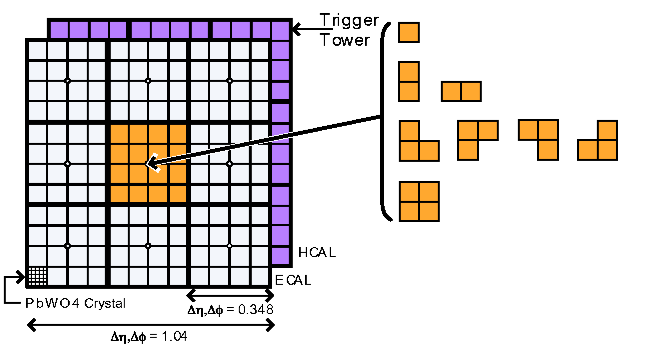
\includegraphics[width=0.5\textwidth]{cms/L1tau}
  \caption{The Level-1 $\tau$ trigger algorithm showing the acceptable $\tau$-like shapes in the central region.~\cite{citeulike:903780}
  \label{fig:L1tau}}
\end{figure}

The Level-1 trigger has separate calorimeter (regional and global) and muon triggers, that are all fed into a global trigger. The regional calorimeter trigger readouts both the ECAL and HCAL calorimetry in coarse grained samples of one HCAL tower or $5\times5$ ECAL barrel crystals, which corresponds to an area of $\Delta\eta \times \Delta\phi = 0.087\times0.087$. The regional calorimeter trigger identifies jet, photon and electron candidates (primitives).

The Level-1 jet trigger sums energy in a $4\times4$ array of towers which are then combined into a $3\times3$ array. Thus a jet is formed from a $12\times12$ array of towers corresponding to approximately a square unit in the $\eta-\phi$ plane. Separate lists are made of central and forward jets. The Level-1 $\tau$ algorithm (Figure~\ref{fig:L1tau}), is similar to the jet algorithm but requires an isolated narrow energy deposit in the central $4\times4$ tower array.  

The Global Calorimeter Trigger (GCT) combines the information from the regional calorimeter triggers and creates an \ET ordered list of each primitive type. The global Level-1 trigger combines the information from the GCT and muon trigger and uses threshold cuts on the primitives to make the accept/reject decision. 

Once accepted by the Level-1 trigger the event is readout and combined by an event builder via a switched network capable of a data transmission rate of 1 TB/s. Once combined the event is sent to a processor in the compute farm, which runs the HLT algorithms and makes the accept/reject decision. Scalability of the system is ensured with the addition of additional event builders and processor units which use the high speed network to communicate. As such during the low luminosity phase only a fraction of the total system will be implemented. As the data rate increases more event builders and processing nodes will be added.

By using a pure software high level trigger maximum flexibility of the reconstruction and triggering criteria can be achieved. The HLT rejects events as soon as possible by using the minimum of event information and by performing partial event reconstruction. Full granularity calorimeter information is used, followed by the tracker pixel detector and finally the full event is reconstructed using all detectors. If an event passes the HLT it is passed to the offline computing system together with a list of all primitives that passed the thresholds, the trigger bits.


% Grid chapter
\chapter{The Grid and the LCG}

\section{Introduction}
The computing requirements for the LHC are unprecedented. By 2010 CMS alone will require over 60\,PB of storage and 100\,MSI2000~\cite{citeulike:847987} of processing power~\cite{CMS_TDR_PHYS_vol1}. At LHC inception no single computing centre was capable of providing these levels of resources. A mechanism for grouping the resources of multiple centres was required. The grid paradigm popularised by Ian Foster and Carl Kesselman~\cite{citeulike:340626} described such an architecture.

The grid was designed to provide an advanced computing infrastructure suitable for collaborative problem solving within science and engineering. Resources, both computational and storage, were shared amongst collaborating institutions within a dynamic Virtual Organisation (VO). The VO comprises individuals based at different institutions around the world all working towards a common goal. The ultimate aim of grid computing was to provide ubiquitous access to resources such that the user did not need to know where their work was carried out. They simply interacted with the grid and resources were provided. The grid was named by analogy with the power grid: users should consume computing power much as they consume electricity, without knowing the details of how or where it was generated.~\footnote{The concept of computing evolving into such a utility was first popularised by Martin Greenberger in 1964~\cite{citeulike:833641}.}

\section{The LCG}
By the year 2000 no appropriate large scale computational grid existed and so work on a custom-designed solution was started. This resulted in the European DataGrid (EDG)~\cite{citeulike:899441} project which was later succeeded by the Enabling Grids for E-sciencE (EGEE) project~\cite{citeulike:899447}. The LHC Computing Grid (LCG)~\cite{LCG_TDR} was originally based upon the EDG and later the EGEE  implementations plus components from VDT~\cite{vdt}, iVDGL~\cite{iVDGL}, Griphyn~\cite{griphyn} and Datatag~\cite{datatag}~\footnote{Other grid implementations existed i.e. Open Science Grid (OSG) in the USA and NorduGrid in Scandinavia and were used by the LHC experiments. Now they are part of the WLCG (Worldwide LCG).}. This chapter describes the EDG and LCG projects as they were in 2004--2005 when the work described in chapters 5 and 6 was carried out.

\begin{figure}[tb]
  \centering
  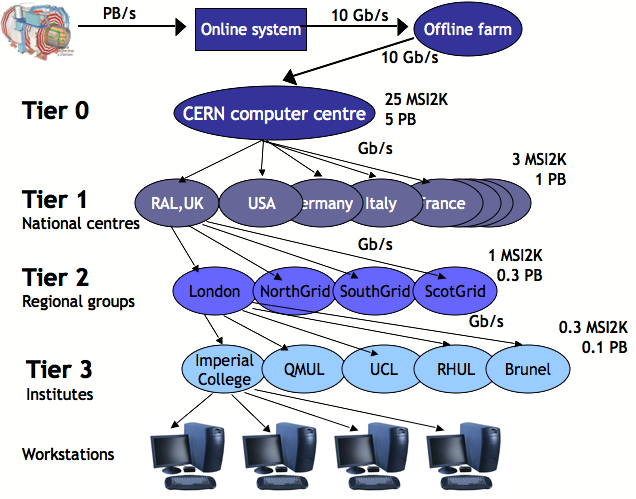
\includegraphics[width=0.9\textwidth]{grid/monarc}
  \caption{The MONARC tiered hierarchy. Network bandwidths are shown for inter-tier links as are computational and storage (disk only) resources for each site in a given Tier. From~\cite{citeulike:421138}.
  \label{fig:monarc}}
\end{figure}

Within the LCG institutions were grouped into a hierarchy derived from the scheme devised by the Models of Networked Analysis at Regional Centres for LHC Experiments (MONARC) project~\cite{Aderholz:2000nk}. This hierarchy took the form of a pyramid (illustrated in Figure~\ref{fig:monarc}) with CERN at the top level (Tier-0). The second level comprised large national computing centres (Tier-1's) followed by regional centres (Tier-2's) and smaller institutes (Tier-3). At each level the resources at a given site decreased, but the number of such sites increased to compensate, from 1 Tier-0 to $\sim$10 Tier-1's, $\sim$50 Tier-2's and an even larger number of Tier-3's.

\begin{figure}[tb]
  \centering
  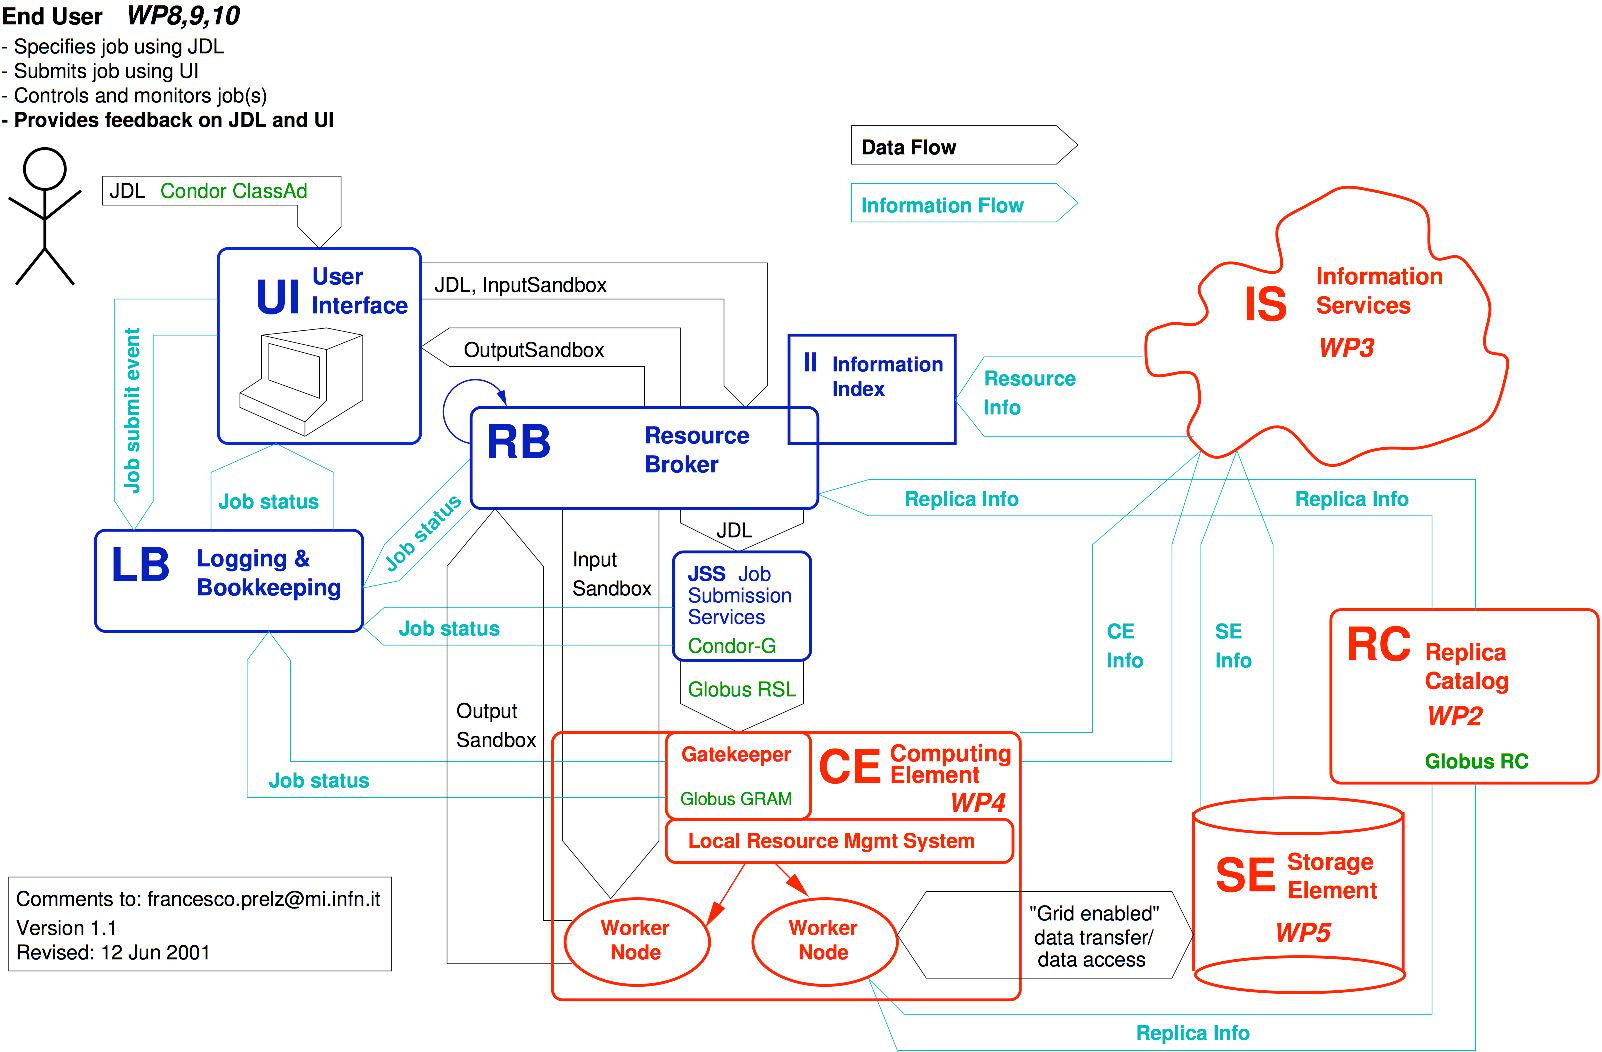
\includegraphics[width=1\textwidth]{grid/LCG-architecture}
  \caption{An overview of the major LCG components. From ~\cite{citeulike:833648}
  \label{fig:LCG-architecture}}
\end{figure}

To provide interaction between users and components a complex software (middleware) architecture was required, as can be seen in Figure~\ref{fig:LCG-architecture}. The User Interface (UI) was the gateway to the grid for users. The installed software allowed the user to manage data and submit computational jobs. 

Data was stored on a site's Storage Element (SE) and recorded in a global file catalogue, known as the Replica Location Service (RLS) or Replica Catalogue. By using the client tools a user could copy data to/from and between SEs. Queries on the RLS were used for data discovery and location.

The Workload Management System (WMS) was provided by the Resource Broker (RB). The RB's role was to accept users' jobs and take responsibility for assigning them to a site for processing. The Computing Element (CE) controlled the processing at a site, receiving jobs from the RB and scheduling them for execution on the site's Worker Nodes (WNs). The Logging and Bookkeeping (LB) system recorded changes in job state and was queried by users to determine the state of their jobs.

The Information Services (IS) listed all the RBs, CEs and SEs and was used by each system, and end users,  to discover and obtain information about the other components.

%%%%%
%Data Management (DM) was provided by the Replica Location Service (RLS) with files stored in Storage Elements (SE). The Information Services (IS) listed all the RB's, CE's and SE's and was used by each system to discover and query other components.
%%%%%

\subsection{Data Management}
The LCG data management system was specifically designed to cope with the types of data produced by particle physics experiments: i.e. large amounts of read-only data. It had also been designed to provide high levels of data availability and integrity with multiple distributed file replicas. To facilitate this the RLS provided the concepts of Logical File Name (LFN), the canonical name by which a file was known, and Physical File Name (PFN), a name referring to a specific file instance. A user would refer to a file by its LFN, the RLS would resolve the best replica and this instance was used in the data operation. As well as holding the LFN/PFN mapping the RLS could also contain a limited number, O(10), file metadata fields. It was generally assumed that files within the RLS were read-only so synchronisation between replicas was not supported.

%LCG's policy was to send jobs to data: if a job required a certain file it was sent to a site which held a copy. This was achieved by the user specifying the required LFN with the job and the RB querying the RLS to find the replica PFNs and hence hosting sites. The RB then submitted the job to one of those sites.

\subsection{Workload Management}
To submit a job the user first had to describe their job in a Job Description Language (JDL) file~\cite{citeulike:835506}.  This file was written in the Classified Advertisements (ClassAds)~\cite{citeulike:835507} syntax and listed the job structure and attributes. Fields included information such as executable name and arguments. It was also possible to specify requirements for the job which were used by the RB to determine an appropriate site to run the job. Typical requirements included criteria such as operating system, site capacity and processing time limits. 

In the JDL the user could also specify input and output files. There were two mechanisms for file handling: small files (e.g. log files and text files) were sent with the job whereas large data files were saved to SEs and registered with the RLS. Input (output) files sent with the job were said to be part of the input (output) sandbox. As well as containing the user-defined input files, the input sandbox contained the users executable and an optional file used as standard input for the job. The output sandbox contained the user defined output files and the standard output and error streams from the job.

Once the user had a JDL file they could submit the job via the software on the UI to an RB. The RB received both the job and the input sandbox then selected the most appropriate CE taking into account the specified requirements, a process known as match-making. Once a CE received the job it was added to the local batch queue and scheduled for execution. Before the job started, the WN downloaded the input sandbox from the RB. The user's job was then executed. Once the job had finished the output sandbox was transferred to the RB. Changes in job state were recorded to the LB. This information was then available to the user. The output sandbox was retrievable from the UI.

The WMS interacted with the RLS when the user specified one or more LFNs in the JDL. It was LCG policy to send jobs only to sites which hosted all of the required data. Thus, if a user specified any input LFNs, the RB contacted the RLS, retrieved the list of hosting sites and only considered those in the match-making decision. At the end of the job it could copy any output files to an SE and register them with a user-provided LFN.

%A job could interact with both input and output files. The job could interact with the RLS if the user specified an LFN. It was LCG policy for jobs requiring input data to be sent to a site which hosted all the necessary files. This was achieved by the user specifying the input LFN's in the JDL, these were then available to the RB when it received the job. When the RB attempted to match the job requirements to the available sites it would contact the RLS and only consider sites which hosted all the required data. 

%Files that were not registered could be sent with the job to the CE via the RB, this was called the input sandbox. At the end of the job output files could either be saved to an SE and registered with the RLS or sent back to the RB where they could be retrieved by the user on the UI, this was called the output sandbox.

%Once the user had a JDL file they could submit it via the software on the UI to an RB. The RB received both the job and the input sandbox then selected the most appropriate CE and sent the job to it. Once a CE received a job it was added to the local batch queue and scheduled for execution. Once the job finished the output was handled and the job was sent back to the RB along with the output sandbox. The user could retrieve the contents of the output sandbox, and query the status of their jobs, by using the software on the UI.

\subsection{LCG object persistency}
As well as core grid functionality the LCG project developed related software services for the LHC experiments. One of these was POOL (Pool Of persistent Objects for LHC)~\cite{citeulike:899448} which provided object persistency and file input/output (IO). This system was used by 3 of the LHC experiments, including CMS, in their event data model.

POOL used the LFN/PFN convention and required a file catalogue to store these. This catalogue was used to locate files when users referred to them with an LFN. Multiple file catalogue implementations existed including the RLS, MySQL~\cite{citeulike:835488} databases and XML files. The user had to provide a contact string for a POOL file catalogue before requesting any file operations. POOL provided an Application Programming Interface (API) for queries of the file catalogue. This API allowed queries of LFNs, PFNs and metadata as compared to the native RLS API that was restricted to queries of LFN-PFN only.

When an application used POOL for writing to a file it was automatically added to the file catalogue. When a file was accessed the application/user used the LFN and POOL would consult the catalogue to locate a physical replica to use.

% When saved files were added to the catalogue and they had to be listed before they could be accessed. The POOL file catalogue component consisted of an API and backend technology. The possible backends included the RLS, MySQL and XML files. The same information as in the RLS could be stored in any of these. 

%The POOL file catalogue API allowed queries of LFNs, PFNs and metadata where the native RLS API only allowed LFN/PFN queries. Applications using POOL would use the LFN to specify a file, POOL would use the catalogue to locate a physical replica and use that for all further operations.

This architecture did not make applications grid-aware, however, because files could only be accessed within a site. POOL had no mechanism for resolving the ``best'' PFN or for trying multiple replicas. If a PFN referring to a file hosted elsewhere was returned it would cause the application to fail.

\section{Summary}
The LHC computing requirements were greater than any single site could provide. Therefore the LCG was developed to provide a distributed computing infrastructure for the LHC experiments. This infrastructure provided both data and workload management. However these were not seamless and did not provide all of the necessary functionality. If required, more advanced and custom features had to be implemented by each experiment on top of the LCG. The system developed for CMS is described in the next chapter.

% CMS computing model chapter text
\chapter{CMS Computing Model \label{sec:computing_model}}

\section{Introduction \label{sec:cms_computing_model:intro}}
\footnote{This review has largely been taken from~\cite{CMSNOTE_2004-031} and~\cite{CMS_TDR_PHYS_vol1}.} 
The extensive scope of the computing requirements at each LHC experiment were outlined in the previous chapter as was the need for CMS to develop its own computing infrastructure on top of the LCG. This chapter details the computing model chosen by CMS. 

The CMS computing model lists the 2010 requirements as 116.6 MSI2000~\cite{citeulike:847987}, 34\,PB of disk and 59\,PB of tape~\cite{CMSNOTE_2004-031}. In order to manage these resources effectively a highly developed and scalable computing model was needed. This model had to be capable of managing sufficient levels of resources while facilitating complex particle physics workflows for the non-expert user.

%The extensive nature of CMS's computing requiremernts was outlined n the previous chapter. This chapter refines tese requiremernts and describes the computing model chosen to satidfy these needs. CMS, like all the LHC experiments, with its large quantities of data and computational requirements, needs a highly developed and scalable computing model. By 2010 CMS requires 116.6MSI2000, 34700TB of disk and 59500TB of tape. A well designed management system is needed to make effective use of these resources.

Not all LCG institutions support CMS. Those that do include a large Tier-0 centre at CERN, 7 Tier-1's, $\sim$\,25 Tier-2's and many more Tier-3 centres. CMS also requires an analysis facility at CERN to be available for analysis activities close to the experiment, termed the CMS CERN Analysis Facility (CAF).  

%The nature of the challenge facing CMS computing is exactly the kind of problem the grid paradigm was designed to solve. CMS relies on LCG for its computing infratructure. The CMS grid hierarchy involves a large Tier-0 centre at CERN, 5-10 Tier-1's located at large national computing centres, more than 25 Tier-2's at regional computing centres and many smaller Tier-3 centres hosted by individual universities. CMS also expects a facility at CERN to be available for analysis activities close to the experiment, called the CMS CERN Analysis Facility (CAF).

%%%%%
%In addition to the data flowing from the detector there will be a large amount of Monte-Carlo (MC) simulated data. MC data are being generated before the detector is operational for detector and proof of concept studies and later during CMS operation for comparison with the real data. CMS requires similar amounts of simulated and real data, $\sim1.5x10^{9}$ events/year, this significantly adds to the storage and CPU requirements. In order to effectively utilize these data the CMS computing model includes sophisticated data and workload management systems. 
%%%%%

%%%%%
%%The scale of the problem facing the CMS computing system is vast, consisting of large amounts of data, distributed among multiple geographically separated centres, with hundreds of physicists around the world requiring access to any particular piece. This is the kind of problem that the grid paradigm was designed to solve. CMS follows the general grid architecture of a tiered hierarchy. This hierarchy is distributed geographically and is consistent with the nature of the CMS collaboration, thus allowing CMS to benefit from the resources and expertise which exists at these centres. The CMS grid hierarchy involves a large Tier-0 centre at CERN, 5-10 Tier-1's located at large national computing centres, more than 25 Tier-2's at regional computing centres and many Tier-3 centres hosted by individual universities. CMS also expects a facility to be available for analysis activities close to the experiment, called the CMS CERN Analysis Facility (CAF).
%%%%%

%%%%%
%The Tier-0 is a production facility, it will secure a copy of the detector data, perform first pass reconstruction and stream data to the Tier-1's. The Tier-1's securely store data received from the Tier-0 and perform reprocessing. The Tier-2's receive data from the Tier-1's and allow users to perform batch and interactive analysis. Tier-3 centres will not be part of CMS managed infrastructure and instead will provide resources to CMS on a best effort basis. The CMS CAF will be used for high turn around computing services.
%%%%%

It is likely that the first years of CMS running will be characterised by a poorly-understood beam and detector. As understanding of the beam and detector evolves frequent data reprocessing will be required. During this time LHC operation will be inconsistent and the data flow from the detector will be erratic. Even so there will be great pressure to discover new physics as rapidly as possible, which will require full resource utilisation and the ability to prioritise critical activities.

Due to the expected constraints it has been decided that the computing model, during the startup phase, should be simple, reliable and give the best possible environment for early physics discoveries. The baseline computing model emphasises:
\begin{itemize}
\item Fast and frequent reconstruction;
\item Streamed primary datasets, with distribution and processing driven by priorities;
\item Joint distribution of raw and reconstructed data, allowing wide distribution and direct comparisons;
\item Multiple compact data formats with multiple distributed copies; and
\item An effective and efficient bookkeeping system.
\end{itemize}
There are also plans for beyond-the-baseline architectures and services, which will be implemented once the experiment has stabilised and greater functionality is required. These are not discussed in this thesis.

CMS will operate a structured analysis environment with analysis groups focusing on well-defined objectives whose priority has been determined by the collaboration. Computing resources will be prioritised for different activities; policies at Tier-0 and Tier-1 centres will be set to meet analysis group requirements, whereas controls at Tier-2 and Tier-3 centres will be looser. These controls will be especially important at start-up when only limited resources may be available.

\section{Data Formats}
A canonical Tier-1 lacks the storage capacity for a complete copy of the raw data, so to maximise data availability more compact data formats are to be utilised. This will allow data to be made available for analysis at multiple sites. The formats (data tiers) used are:
\begin{itemize}
\item RAW. This is the output format of the HLT farm. It contains data from all detector channels as well as the Level 1 and High Level Trigger bits. The target event size is 1.5 MB;
\item RECO. This is the output from event reconstruction of the RAW data, where, objects (tracks, vertices etc.) have been reconstructed and calibrations applied. The target event size is 0.25 MB;
\item AOD (Analysis Object Data). This is the output from further reconstruction (reprocessing) of RECO data. Physical objects (electron, photons etc.) have been reconstructed and calibrations applied. This is expected to be the primary data used in analysis. The target event size is 0.05 MB; and
\item TAG. This format indexes other event data and is the output from skimming of event data. This process is used to identify events with similar characteristics. This format has not been implemented to date.
\end{itemize}
When data is collected/produced it is grouped with similar data into datasets. This grouping is driven by the HLT bits. The same dataset may have RAW, RECO and AOD data tiers, therefore both must be specified to identify data uniquely.

\section{Tier roles \& responsibilities}
CMS has assigned each tier within the LCG MONARC hierarchy roles according to their resource levels. The required computing resources at each Tier are listed in Table~\ref{fig:timeprofile}. 

\begin{table}[tbp]
  \centering
  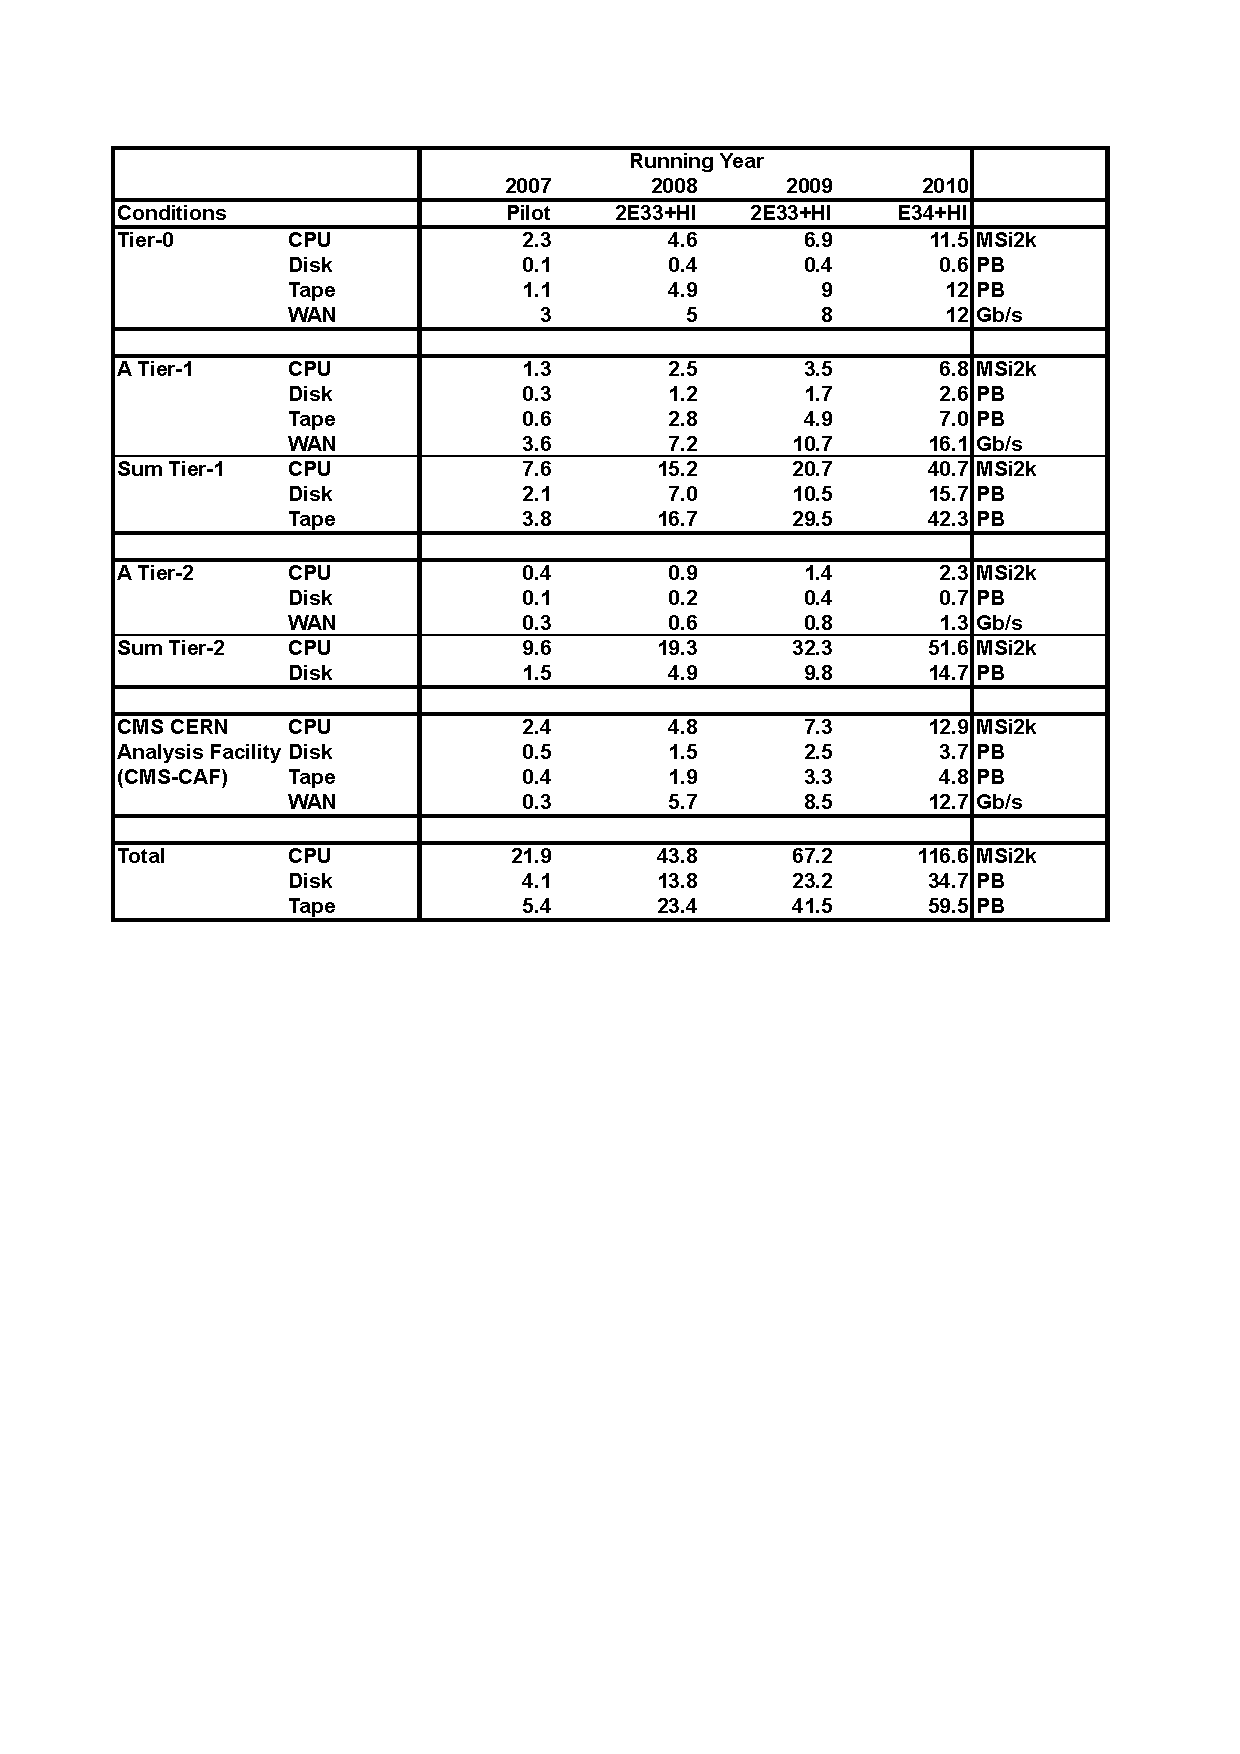
\includegraphics[width=0.88\linewidth]{cms_computing_model/timeprofile}
  \caption{Time Profile of CMS Computing Requirements.~\cite{CMS_TDR_PHYS_vol1} These requirements change frequently, see ~\cite{revised_resources} for up to date figures.
  \label{fig:timeprofile}}
\end{table}

\subsection{Tier-0}
The responsibility of the Tier-0 is to accept data from the CMS online system (HLT). This is then archived, reconstructed and a copy distributed to the Tier-1's. It is essential that this proceeds with minimum delay to avoid a build up of data on the input buffers. Thus the resources of the Tier-0 must be dedicated and continually available. During periods that CMS is not taking data the Tier-0 will be used for heavy-ion reconstruction, which takes $\sim$10-50 times more processing than that of a proton-proton event. %%Thus usage of the Tier-0 is expected to be continuous and is required on a 24/7 basis.

\subsection{Tier-1}
The Tier-1's have a number of responsibilities including secure data storage and centrally co-ordinated processing. The Tier-1's as a whole are responsible for storing the custodial copy of the RAW data with the Tier-0 copy only accessed in the event of data loss. Due to its small size each Tier-1 stores the entire AOD. Both real and Monte Carlo data is included in the Tier-1 storage.

Tier-1 data processing includes reprocessing, skimming and a small amount of analysis. A Tier-1 will reprocess all of its data at least twice a year. A limited amount of well managed analysis will be allowed, probably making use of the RAW data. All activity at the Tier-1 will be managed and subject to CMS control and policies.

\subsection{Tier-2}
The main role of the Tier-2 is to support a portion of the physics community and run analysis jobs. Many detector-specific calibration and analysis groups are expected to operate at a Tier-2 ``close'' to the relevant experts. It is expected that such a Tier-2 would provide extra resources for that group, i.e. extra storage space and relevant software installations. The analysis will originate from both local and remote users. 

A nominal Tier-2 has enough disk space (no tape is required at Tier-2's) to hold approximately one-tenth of the current RECO data and half of the current AOD. Tier-2's have no custodial responsibility for data. Data will be downloaded, analysed and periodically replaced. As well as providing for analysis the Tier-2's must provide processing capacity for Monte Carlo production ($\sim10^{8}$ events per year). These data will be stored at the Tier-1.

%%%%%
%A standard T2 is a single site with all resources located together, however there is another type of Tier-2 site, the federated Tier-2. This Tier-2 may be made of multiple institutions linked together and sharing resources. As long as the Tier-2 is presented to the user as a single entity with appropriate levels of resources the actual configuration of a Tier-2 is left to the local management.
%%%%%

\subsection{Tier-3}
In CMS, Tier-3 sites are users' home institutes, where they are provided with the facility to develop and submit their analysis. The major usage pattern consists of users submitting analysis jobs either to run locally or at a remote site and for the results to be returned to them at the Tier-3. Some Tier-2's will also provide Tier-3-type facilities as well as fulfilling their nominal role as defined by the computing model.

\subsection{CMS-CAF}
The CMS-CAF provides general facilities for the whole collaboration, serves users without a local Tier-1/2 and provides facilities for low latency, experiment-critical activities. General services include user logins, database support, production bookkeeping and software repositories. High priority work, generally taking advantage of the only copy of all RAW data, will include:
\begin{itemize}
\item Detector diagnostics - particularly useful during early running stages and after periodic shutdowns;
\item Trigger performance studies - i.e. optimisation and algorithm development. These studies will be carried out in response to changing understanding of the detector or the need to focus on specific channels; and
\item Calibration and alignment - to support the HLT and to be used in the (re-)reconstruction at the (Tier-1) Tier-0.
\end{itemize}

The analysis facilities offered to users will be approximately equivalent to 2 nominal Tier-2 centres. However, it is essential that individual users cannot interfere with the critical work undertaken here, hence strict policies and quotas will be put in place.

\section{Data Distribution}
The data distribution system must be capable of multiple simultaneous transfers between sites while maximising network usage and ensuring data integrity. Transfers must be automatic, provide for error recovery and conform to priorities determined by the experiment. It is vital that data from the detector be archived and streamed to the Tier-1's with minimum delay and without data loss. Lower priority transfers include data for user analysis being streamed to the Tier-2's. Monte Carlo data generated at the Tier-2/3's must also be moved to the Tier-1 for long-term storage.

The planned data flow for CMS is illustrated in Figure~\ref{fig:streams}. The online system will be set to write out events at the maximum rate that the offline computing model can support, which ties the physics reach of the experiment to the performance of the offline computing system. In the baseline model this rate will be set to a minimum of 225 MB/s giving an event rate of 150 Hz.

If an event passes the HLT it is passed to the offline system. The Tier-0 archives a copy of this data then passes it through a first pass reconstruction that results in RAW, RECO and AOD data products. 

Each Tier-1 receives a share of the RAW and RECO data consistent with their resources and a complete copy of the AOD. Periodically the Tier-1 will reconstruct its RAW data to produce new RECO data and then reprocess that to produce new AOD.

The Tier-2's obtain a share of the RECO data and half of the AOD from the Tier-1. The specific content will vary as physics priorities change and Tier-1 processing progresses. As such, a Tier-2 is expected to be capable of refreshing all of its data within 30 days, corresponding to a data import rate of 5 TB/day.

%datasets will be shared amongst the Tier-1's, which will periodically replace the RECO by performing re-reconstruction of the RAW data as understanding of the detector changes. 


%%%%%
%%For performance reasons events from the HLT are passed in one of $\sim$10 ``online'' streams. A copy is made of these streams and archived at the Tier-0. The online streams are then passed through a first pass reconstruction which results in $\sim$50 datasets containing RAW and RECO data. The reconstruction will initially be performed at the Tier-0 with the Tier-1's carrying out periodic re-reconstruction as understanding of the detector changes. The RAW + RECO datasets will be shared out amongst the Tier-1's with an additional copy archived at the Tier-0.
%%%%%
\begin{figure}[!tbp]
  \centering
  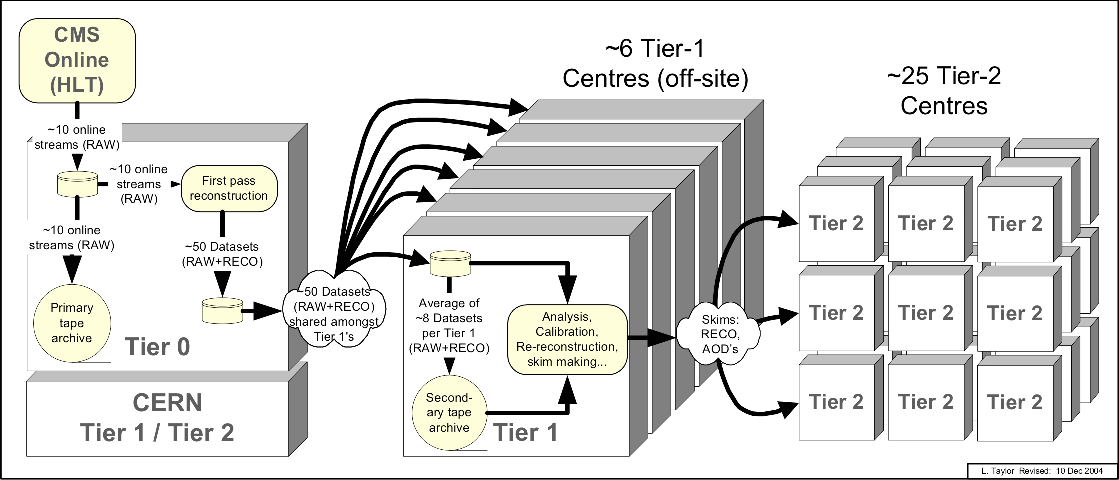
\includegraphics[width=1\linewidth]{cms_computing_model/cms-streams}
  \caption{Schematic flow of bulk (real) event data in the CMS Computing Model.
           Not all connections are shown, e.g. peer-to-peer connections between Tier-1's and Monte Carlo data transfer from the Tier-2 to Tier-1.~\cite{CMS_TDR_PHYS_vol1}
  \label{fig:streams}}
\end{figure}

%The Tier-2's obtain RECO data and half the AOD from the Tier-1 and send back generated Monte Carlo.

%The first copy of the AOD is be produced at the Tier-0 as an adjunct to the main first pass reconstruction step. The Tier-1's are then responsible for periodically reprocessing their RECO data to replace the existing AOD. The entire AOD is to be distributed to all Tier-1's as well as half to each Tier-2. Data flow to the Tier-2's will consist of both RECO and AOD datasets. With MC data flowing from the Tier-2 to Tier-1.



%\section{Examples of user activities}
%Here three potential use cases of the computing model are presented. They are taken from~\cite{CERN/LHCC-2005-023} and are intended to show how the computing model will satisfy the needs of the collaboration.

%\subsection{Mainstream analysis}
%A member of the Higgs Physics Group in 2009 is searching for the SUSY Higgs in a particular decay channel. The collaboration has judged this to be a high priority search and the group has been allocated resources at several Tier-2 centres to carry out their work. The Tier-2's made available to the members of the group will not always be the closest to a particular member. However it is likely that physicists in the same group will be allocated resources close together to allow shared usage of data and storage space.

%Periodically the group will ask for a modest amount of AOD or RECO data to be transferred to their Tier-2 to allow it to be analysed. If the data is not at their 'local' Tier-1 centre it will be copied to the Tier-1 and then to the Tier-2 transparently, possibly taking a few days. The group may put in a request for officially generated MC. Once accepted this request is scheduled centrally and constituent jobs are run at Tier-2 and Tier-3 centres around the world. The resulting events are copied to the local Tier-1 and Tier-2 centres. Here they are available to other members of the collaboration. 

%If the group requests a high priority analysis of data at multiple Tier-1 sites, and collaboration management approves, jobs will be scheduled at the relevant Tier-1's. If these jobs are given a higher priority than re-reconstruction which may already be running, the re-reconstruction jobs will be migrated to the Tier-0. If the group requires higher statistics they may request that Tier-1 centres skim events in the first pass AOD as they arrive, creating a new dataset. This new dataset may then be streamed to the Tier-2 where analysis may be performed on it.

%\subsection{Calibration study}
%A CMS physicist is a member of a group that is responsible for monitoring and calibration of the ECAL detector. In this role the group runs Data Quality Management (DQM) jobs to check that the prompt calibration system at the CMS-CAF is operating correctly. It is important that this system is operating correctly as the results are fed back to the first pass reconstruction within an hour of data taking. In order to monitor this process a sample of events are analysed from the reconstructed data. This is ensured by using a high priority but low statistics express stream which is analysed with low latency at the CMS-CAF.

%Due to a problem the calibration system fails over a period of a few days and the correct calibration constants are not used during first pass reconstruction. Before this problem is fixed the events are distributed to the Tier-1 centres. Since the ECAL calibration is critical for multiple analyses the collaboration decides to perform a second pass reconstruction on the affected events. This is performed at the Tier-1 centres with a high priority. 

%As a result the calibration group develop a new version of their algorithm but need access to a very large event sample to test it. They put in a request to the collaboration to run over a large amount of RAW data, this is approved with a medium priority, and their jobs run at the Tier-1 centres over the next few weeks. Once they are satisfied with the new algorithm it can replace the old one in the mainstream reconstruction.

%\subsection{Hot channel}
%A physicist is interested by a new GUT formalism that predicts a certain event signature and tries to look for it. The relevant group has limited resources and assigns this search a low priority. The physicist has access to resources at his local Tier-2 and uses them in his search, he requests a transfer of relevant AOD samples, this again is set at a low priority, and slowly the events are transferred. The physicist carries out his study and does indeed find the signature he is looking for, he contacts colleagues and ascertains that they to see the same signature on the same data at the Tier-2. Other members of the analysis group then begin to get interested and resources at the Tier-1 are assigned for a more thorough search in the RECO data. The interest becomes such that the centre becomes heavily loaded and therefore the events are replicated to another Tier-1 to make more resources available.

%The interest is so high in this work that the event signature is added to the express channel at the Tier-0 and analysis jobs run over the RECO data at the CMS-CAF as soon as possible. The result of all this interest is that a bug is found in the CMS trigger. This places a lot of physics results in doubt hence the impact must be determined quickly. Therefore the collaboration takes the decision to devote all available resources to reprocessing selected datasets. The computing policies are rapidly changed to accommodate this. As a result the first pass reconstruction is not carried out in real time instead the data is stored at the Tier-0 and Tier-1 for later reprocessing. This leaves capacity at both the Tier-0 and Tier-1 available for re-reconstruction. The Tier-2 centres are then used by selected physics groups to carry out their analyses. Once the reprocessing is complete the Tier-0 and Tier-1 centres resume normal operations with additional resources being scheduled at the Tier-1's for reprocessing until the backlog is under control.

%%%%%
%\section{MC production?}
%???
%%%%%

%%%%%
%\section{CMS policies}
%The CMS competing system is composed of a large number of semi-autonomous centres, operating with different policies and resources. These resources may be shared amongst multiple experiments and scientific disciplines. It is required that the resources allocated to, and used by, CMS be accounted for.
%
%It is the goal of the CMS computing system to allow maximum flexibility and freedom to its users. However this is likely to be offset by a high contention for resources, especially during the early running period. Therefore CMS requires the ability to set policies determining data placement and resource usage. These policies are expected to change rapidly as the collaborations priorities change. Any CMS user must be potentially able to use any CMS resources with a priority set by the collaboration.
%%%%%

\section{Computing Services}
CMS has developed the following guiding principles for its computing services:
\begin{itemize}
\item Optimise for read access. In general CMS data will follow the general HEP pattern of being created, never modified and subsequently read many times;
\item Optimise for the bulk case, while still allowing basic tasks. In CMS the large amounts of data and jobs will require operations on a large scale i.e. the data transfer will be managed at the dataset level. However the functionality still exists for users to copy individual files;
\item Minimise dependencies of processes on the worker nodes (WNs). CMS expects $10^{3} - 10^{4}$ worker nodes to be in constant use. This presents a large reliability problem as nodes fail or suffer outages. The WN is made more reliable by removing as many external dependencies as possible. Any dependencies that do remain should be local to a site to avoid any single point of failure for the entire system;
\item Allow provenance tracking. It is a requirement of the software and computing frameworks to track the provenance of datasets. This includes run-time parameter sets and software versions;
\item Site configuration information should remain local to the site. This allows system administrators to setup their site however they wish while allowing CMS applications to discover any information required; and
\item Keep the solution simple. The start-up of CMS is likely to be a hectic and confusing time, thus it has been decided that the computing system should be as simple as possible while providing all necessary functionality.
\end{itemize}

The CMS computing system consists of a distributed set of systems and services. These services consist of a mix of generic grid, site-specific and CMS-specific components. Figure~\ref{fig:comp_arch} shows the major components of the computing system. The main systems are:
\begin{itemize}
\item Data Management System - the CMS data management and movement tools.
\item Grid Workload Management System - the core grid systems and services of which CMS makes use.
%\item Other CMS specific services. 
\end{itemize}

\begin{figure}[!tbp]
  \centering
  \vbox{
    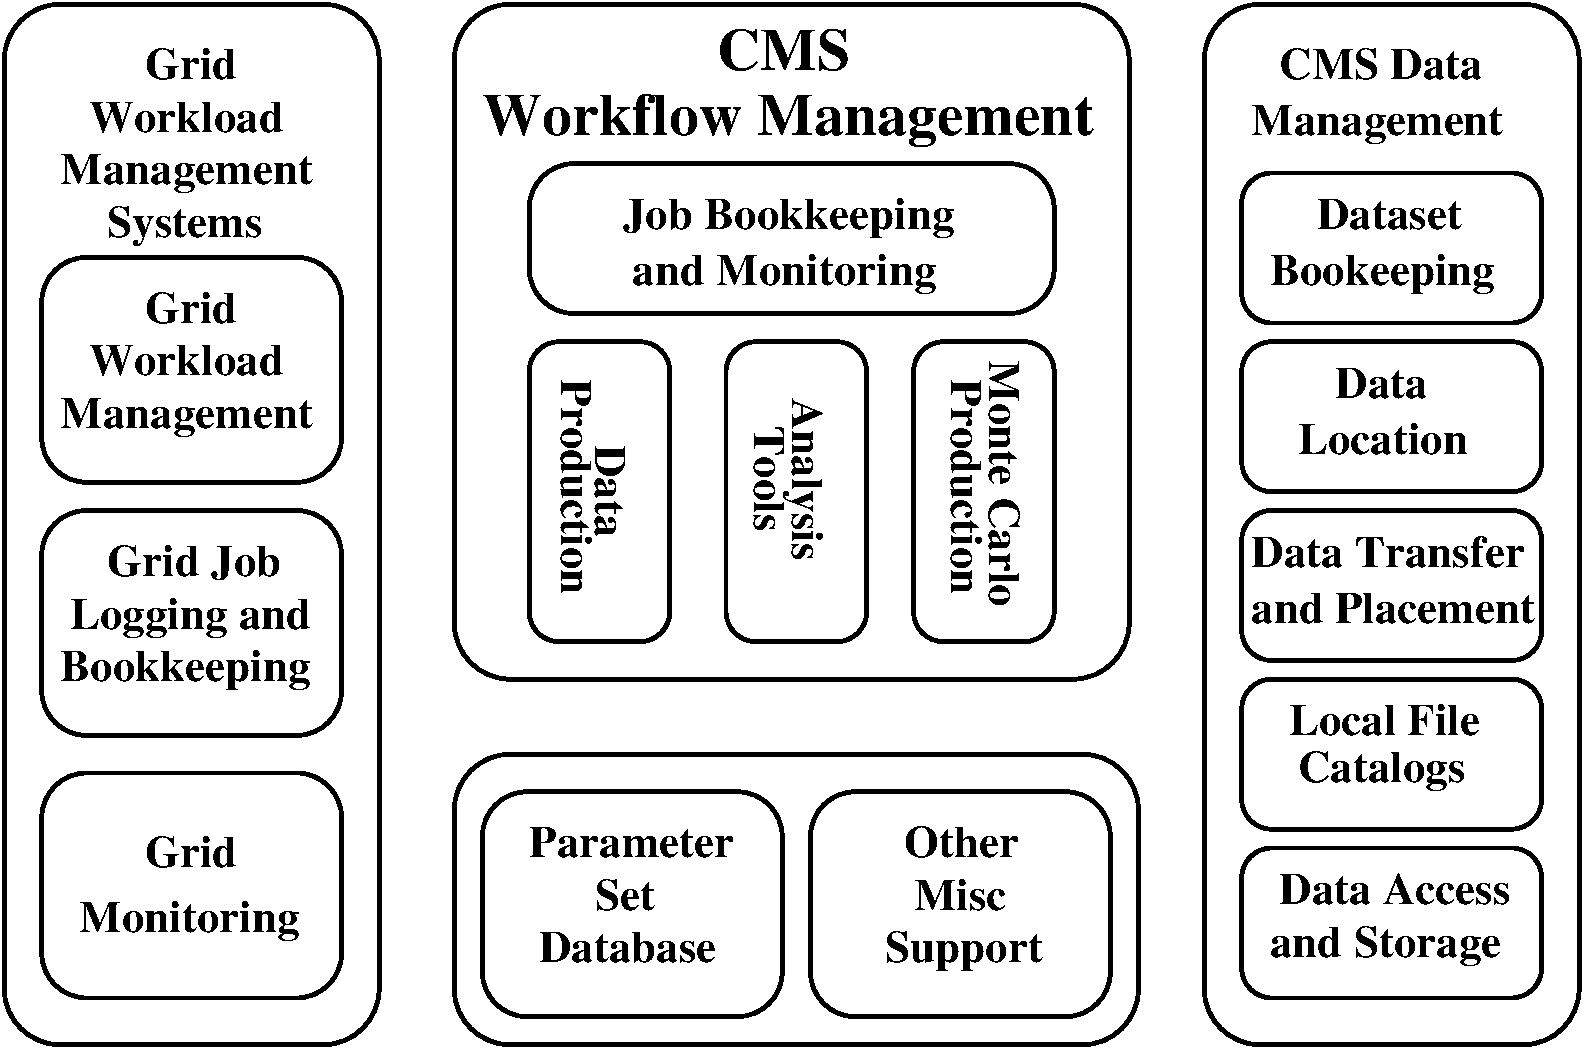
\includegraphics[width=0.95\linewidth]{cms_computing_model/global_architecture}\\[1mm]
    \caption{Overview of systems and services supporting the CMS workflow
           management system.~\cite{CMS_TDR_PHYS_vol1}
    \label{fig:comp_arch}}
  }
\end{figure}

These pieces are tied together by the CMS Workflow Management (WM) system. This system supports all necessary workflows in CMS, including (re-)reconstruction, reprocessing, calibration, MC production, skimming and user analysis, while shielding users from the complexity and implementation details of the underlying components. 

\section{Data Management System}
%\subsection{Introduction}
The CMS Data Management (DM) system is designed to provide necessary data management functionality for CMS, i.e. allowing physicists to discover, access and transfer various forms of data. These facilities will be used in situations ranging from organised large-scale data placement operations to individual user file transfers. The system must be suitable in all situations.

In the baseline model the experiment data placement will be pre-determined leaving the CMS WM system to steer jobs to the correct location. The DM system will provide functionality for the WM system to accomplish this. 

The Data Management system understands both user-oriented terms such as dataset as well as technical details such as file names that need not necessarily be exposed to the user. An ``event collection'' is defined as the smallest data unit that may be selected. A dataset is defined as a set of ``event collections'' that share a set of trigger bits. The dataset concept is used by physicists to specify data for their analysis jobs, but the jobs will be configured with, and at run time refer to, event collections. Event collections are stored in files that are themselves grouped into ``file blocks''. These file blocks are groups of files that are generally distributed and accessed together.

The DM architecture is based on a loosely-coupled set of components, which together provide the functionality required of the system. The basic components of the system are:
\begin{itemize}
\item Dataset Bookkeeping System (DBS) - lists the available data. For the physicist this will be the primary means of data discovery. The DBS can be queried with criteria such as run range, data tier, software version and data quality flags. Results will be returned as either datasets, event collections or file blocks. These can then be used to configure the CMS analysis framework;
\item Data Location Service (DLS) - maps file blocks to sites. Queries will result in a list of sites that contain the given data;
\item Data Placement and Transfer System - handles file transfers. The data placement system will be used to manage data movement and placement. File blocks will be subscribed to sites and the request passed on to the data transfer system. The data transfer system will handle reliable end-to-end transfers of individual files;
\item Local File Catalogue - provides file lookups at a site. This catalogue presents a POOL interface that is able to return file locations at a site and can be used by CMS applications to locate event data. In the current implementation this is a text file that contains lookup rules to determine the correct file location; and
\item Data Access and Storage System - provides access to files and manages the local mass storage system, if any.
\end{itemize}

%%%%%
%*FIXME* Wanted?
%The Data Management system handles many levels of complexity *FIXME* from the global bookkeeping of the experiment to the moving of files local to a site. CMS splits this into two ``scopes'': global and local. The global scope is taken to mean the system used by physicists to find which data is available. These services will run at the Tier-1 and Tier-2 and will have well defined contact points known to the collaboration. Local scope refers to data created and accessed by a sub-set of the collaboration, this includes ``private'' data and MC production that has not yet been published to the global scope. In the local scope not all the DM system components will be required. It may be possible to ``publish'' data from a local scope to the global one, this would allow users to create their own data, validate it and make it available to the collaboration.
%*FIXME*
%%%%%

%The Data management system supports user oriented terms such as dataset and technical details such as files. An ``event collection'' is defined as the smallest data unit that may be selected. A dataset is defined as a set of ``event collections'' that are naturally grouped together. The dataset concept is used by physicists to specify data for their analysis jobs however the jobs will be configured with, and at run time use, event collections. Below the view of event collections are physical files. In CMS the packaging of event collections into files will be done in such a way as to have an average file size of at least 1 GB, as mass storage systems have scaling issues with small files. CMS also defines the term ``file block''. This is a set of files that will generally be accessed and transferred together and is expected to be in the range 1-10 TB for data management reasons.

%\subsection{Dataset Bookkeeping System}
%The Dataset Bookkeeping system (DBS) provides a mechanism for querying the event data. For the physicist it is intended to be the primary means of ``data discovery''. The information returned from the DBS will be site independent. Typical operations are expected to involve selecting datasets and defining new datasets from selected events in other datasets. Datasets may be searched for using criteria such as run range, data tier, software version and data quality flags. Once selected a list of event collections are returned to allow analysis or production job configuration. Similarly the DBS will provide the mapping from event collections to files and file blocks. 

%%%%%
%The DBS also provides information about provenance tracking of collections such as the event collections it is derived from, software versions used during reprocessing and MC generation. The DBS may also contain summary information of the collections it holds, i.e. estimates on the integrated luminosity, information on the runs including possible data quality flags. The DBS will not track job bookkeeping, MC requests etc. these will be stored by the WM/Production bookkeeping systems.
%%%%%

%%%%%
%It is expected that the DBS will be available in several forms. The global scope will be satisfied by an instance at CERN with mirrored copies at other locations to aid access. It is also possible that a DBS may be in use at an institute with local scope, containing details about private data. The DBS is a VO specific service that describes CMS data in terms of datasets and data blocks and so will be constructed by CMS on top of grid services.
%%%%%

%\subsection{Data Location Service}
%The Data Location Service (DLS) is used to find out where instances of data exist. This maps file blocks to storage elements. It is likely that the DLS will be implemented as a two tier system, a local DLS instance will publish the data-blocks available and a global instance aggregates the information from the local instances. Queries to the global DLS will result in a list of sites that contain a given data-block.

%The file catalogues are expected to provide file attributes such as file size and checksums but will not contain any CMS specific attributes. The catalogue is expected to be highly scalable and to be as robust and reliable as the data storage.

%\subsection{Data Placement and Transfer System}
%The data placement system is used to define, execute and monitor CMS policies on where data is to be located. This layer manages the allocation and release of storage resources and data transfers at the dataset level. The data transfer system handles reliable background transfers of files from multiple sources to multiple destinations at maximum data rates. 
%The data placement and transfers systems are implemented by the PhEDEx project. *FIXME* REF

%%%%%
%The requirements on such a system include a managed and structured data flows, multiple transfer modes and priorities. The CMS data flow is highly structured with data flowing from the Tier-0 through the Tier-1's to the Tier-2's. This kind of data flow is required as the Tier-0 could not cope with all sites connecting directly to it. The system must be able to track file transfers as they move through the different tiers and know when the data has reached its final destination and be able to release any temporary copies used during the transfer.
%%%%%

%Data transfers need to occur in different modes, the Tier-0 will push data out to the Tier-1's continuously, but must dynamically re-route data if one of them becomes unavailable. Tier-2 sites will want to subscribe to datasets that interest local physicists and here the data is pulled from the Tier-1's. All of these transfers must take place with the appropriate priorities set, obviously data streamed from the Tier-0 should be moved with a higher priority than a request from a Tier-2.

%The data placement service keeps track of file-blocks and subscriptions. A subscription request specifies the data to be transferred, the priority and whether the resulting copy should be considered as the custodial one (i.e. in the case of MC data transferring form a Tier-2 to Tier-1.

%The data transfer system operates at the file level, it receives assignments from the data placement system. It then handles the end to end transfer reliably using one of a group of tools depending on individual site configuration.

%\subsection{Local File Catalogue}
%The DLS provides the site and storage element that hosts an event collection but not individual file locations. The physical location of files is only known within a site by the local file catalogue. This catalogue presents a POOL interface which is able to return the physical location of a file based on it's logical file name or GUID. CMS applications only know about logical files and rely on the file catalogue to locate them.

%\subsection{Data Access and Storage Systems}
%The data transfer system in CMS expects an SRM interface to the mass storage system. This interface allows for file transfers, space allocation and deletions. Larger sites will be expected to provide secure storage, probably tape based, with large disk caches to allow applications to access the files. CMS applications require POSIX-like~\cite{citeulike:363700} file access.

\section{CMS Workflow Management System}
\subsection{Introduction}
The CMS Workflow Management (CMS WM) System combines the CMS DM and grid workload management systems and presents them in a uniform manner to the user. The WM system includes applications designed to support all major CMS workflows including prompt reconstruction, prompt calibration, re-reconstruction, reprocessing, calibration, Monte Carlo production and analysis.

The primary unit of work in the WM system is a task. The task contains an application, configuration parameters and optionally a data selection. The DBS and DLS search for the data selection and once the WM system discovers the nature of the data to run over, i.e. number of runs/events, it can decide how best to run the workflow. In general, the task will be split into many jobs each running over a subset of the total requested data. Once the individual jobs have been created they are submitted to a supported grid WMS. This then takes responsibility for scheduling the job at an appropriate site, i.e. one that contains the required data. Once the job is finished the CMS WM system will retrieve the results and handle any output files. 

Figure~\ref{fig:WM_general} shows how the CMS DM system and the grid WMS are combined. The UI is the gateway to both the grid and CMS WM system with both CMS WM applications and grid tools installed. Individual CEs and SEs in supported grid middlewares advertise themselves via their native information services. The CMS WM system can then run a given workflow on the most appropriate resources on any supported grid middleware. 

\begin{figure}[tbp]
  \centering
  \vbox{
  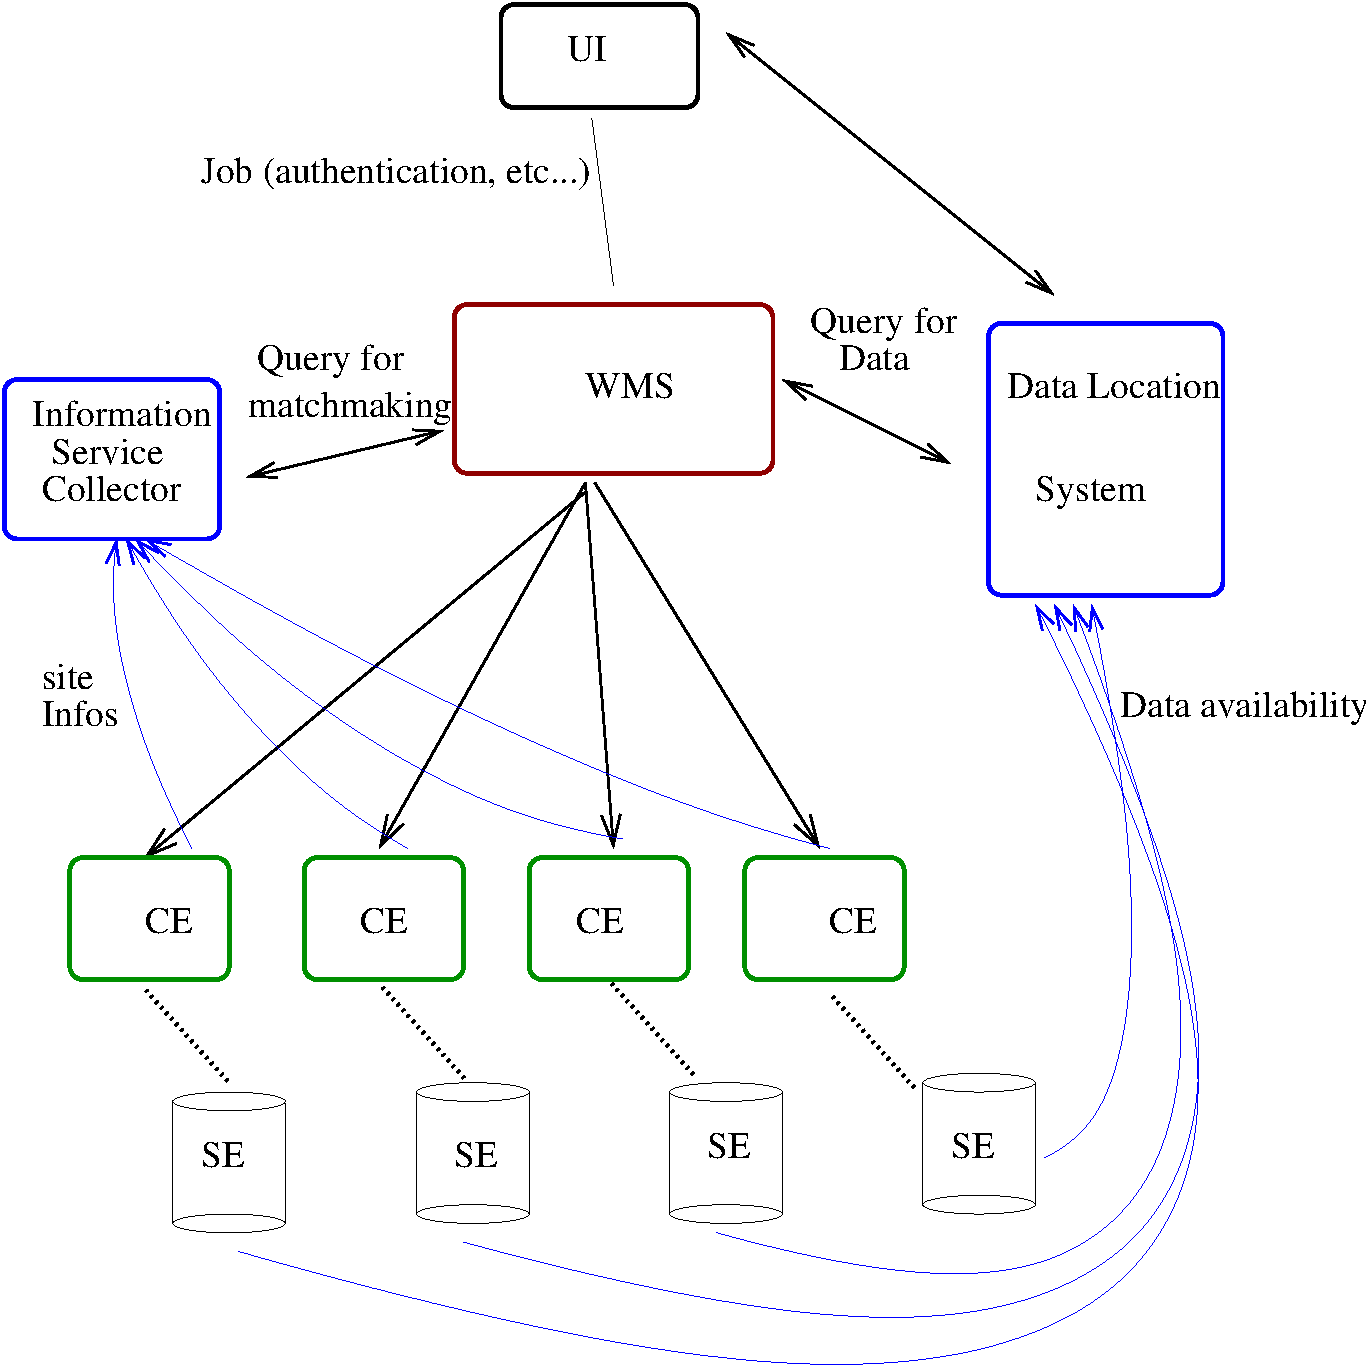
\includegraphics[width=0.65\linewidth]{cms_computing_model/Grid_WMS_base}
  \caption{The baseline CMS WM system architecture.~\cite{CMS_TDR_PHYS_vol1}
  \label{fig:WM_general}}
  }
\end{figure}

The work of the CMS WM system is simplified for workflows that run exclusively on the Tier-0 (prompt calibration and reconstruction) as no grid middleware is needed. 

\subsection{User analysis}
One of the prime supported CMS workflows is that of user analysis. These analyses are carried out by individuals or groups of physicists and will be the source of physics discovery at CMS. All data taken by CMS will be analysed many times by different groups, each looking for different physics. Classic CMS analysis, described below, limits the user to running over local data and requires the user to handle job creation, submission and output file handling. The CMS WM expands on this by providing full automation from analysis creation through to job splitting and output file handling.

%The CMS WM system (see Figure~\ref{fig:WM_analysis}) will provide a common interface to all grid implementations. For user analysis the CMS WM system takes a users analysis task and uses the grid infrastructure to submit it as multiple batch jobs to appropriate sites, i.e. ones that hosts the required data. Functionality includes data verification, site location, job splitting, packaging, submission and output retrieval. The CMS WM system is capable of interfacing to multiple types of batch system, both local and grid.


\subsubsection{Classic CMS Data Analysis}
Analysis of event data is performed with the CMS analysis framework. This provides a layer of common functionality (event access, reconstruction algorithms, calibrations etc.) that users may call on in their analysis programs. Users build their code against this framework and an executable is produced. This executable dynamically links with the framework libraries as extra functionality is required. User options, datasets and other parameters are passed via a configuration file. In CMS the standard practice is for the user's analysis code to produce an ntuple file that is then analysed with ROOT~\cite{citeulike:363715}, or similar a tool, to produce final plots.

The framework utilises POOL for file IO and catalogue functionality. The CMS analysis framework refers to data files via their LFNs and relies on POOL for file location and IO. This means that to run in the framework, the user has to specify, in their configuration file, at least one POOL catalogue that contains the required event files. The framework has no knowledge of the grid as it runs locally and assumes that files in the POOL catalogue are accessible. Users can only therefore analyse data at their local site, which is clearly incompatible with CMS's distributed data model. The CMS Workflow Management System solves this problem and provides the user with access to all CMS data and computing resources.

\subsubsection{Distributed User Analysis Workflow}
The classic analysis scenario is useful for developing analysis code and analysing small numbers of events. However most CMS analyses require running over thousands or millions of events. To do this a user has to write their own machinery to create possibly hundreds of analysis jobs then submit them and finally handle the hundreds of resulting output files. This process is tedious and prone to error.

A main function of the CMS WM system is to simplify and automate these functions for the user. Functionality includes data verification, data location, job splitting, packaging, submission, output retrieval and merging. This workflow is illustrated in Figure~\ref{fig:WM_analysis} and presented below.

\begin{figure}[tbp]
  \centering
  \vbox{
  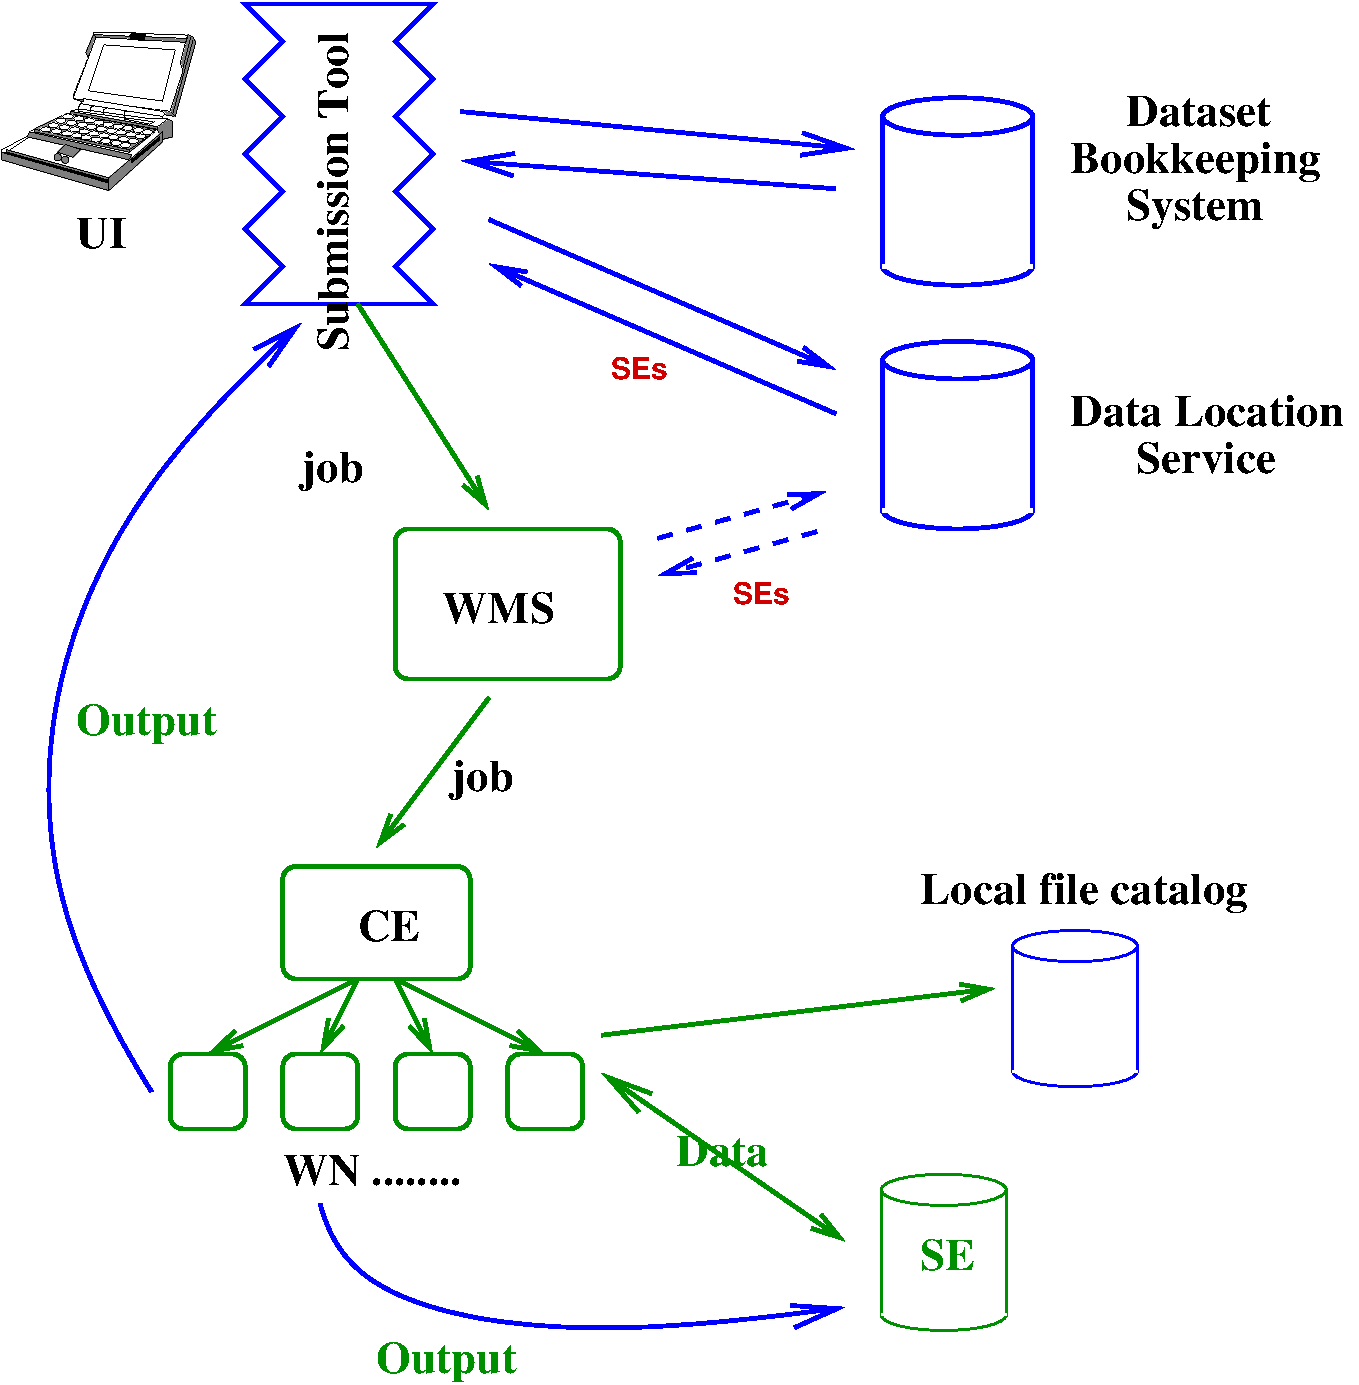
\includegraphics[width=0.65\linewidth]{cms_computing_model/WM_analysis}\\[1mm]
  \caption{Distributed data analysis with the CMS WM system.~\cite{CMS_TDR_PHYS_vol1}
  \label{fig:WM_analysis}}
  }
\end{figure}

%A major function of the CMS WM system is to manage user analysis. It takes a users analysis   For user analysis the CMS WM system takes a users analysis task and uses the grid infrastructure to submit it as multiple batch jobs to appropriate sites, i.e. ones that hosts the required data. Functionality includes data verification, site location, job splitting, packaging, submission and output retrieval. The CMS WM system is capable of interfacing to multiple types of batch system, both local and grid.

%A main function of the CMS WM system is to transform a user analysis task into a set of jobs to be run on the distributed computing system and to manage and log the relevant details. Here a typical user analysis workflow is presented.

The user begins (as in the ``classic case'') with an analysis application they wish to run, various configuration options and the data they wish to run over. These data may either be a named dataset or determined from a list of requirements i.e. software versions and HLT flags. The DBS is then contacted and the required data determined. This query results in a list of available event collections (and file blocks). The WM tool is then able to decide how best to divide up the user's analysis task into multiple jobs, each of which accesses a subset of the total data. The job splitting is driven by the user's configuration (maximum events per job, desired job run time etc.). 

The CMS WM system can then create the configuration for the jobs. This is a two step process as each job is configured at the CMS application level and at the grid WMS level. The application configuration requires the input event collections. The grid WMS configuration needs information in order to steer the job to a site that holds the appropriate event collections. This is accomplished by contacting the DLS to discover which storage elements (SEs) contain the required data. The user may specify that the output be returned directly to them or, if the output is likely to be large or accessed by others, copied to a remote storage element.

%%%%%
%The CMS WM system is now able to submit the users jobs. Until interoperability between the different grid WMS has been achieved the decision of which grid to use must be taken at submission time. Using the DLS the CMS WM tool can determine which grids have access to the data, if only one of them does then the decision about which grid to submit to is trivial. If more than one does the users preferences may be taken into account. When interoperability between grids is achieved the jobs will be submitted to a general service capable of steering their job to whichever grid is most suitable.
%%%%%

The CMS WM system submits, and tracks jobs to the WMS, or local site batch system. Jobs submitted to distributed resources are sent with a list of SEs that contain the requested data blocks and it is the task of the grid WMS to steer the job to the ``best'' site in terms of load, data access cost etc.

Once a job arrives at a site and locates the site-specific information, the user's application is presented with an environment that is identical to the development setup. This includes such things as CMS software installations and access to the CMS conditions DB. Once all of these have been found, the user's application runs exactly as during development with files streamed from the local storage system by use of the local file catalogue.

The user tracks their jobs using the CMS WM job logging and bookkeeping system, which uses the WMS information services as an information source. Optional real-time monitoring allows the user to monitor the progress of the job including such information as event number and CPU usage. This is optional as it requires the site to allow information to be sent from the job to an external service. The user may also find this unnecessary, especially if they have a large number of active jobs. Once the job finishes the output is either saved to an SE or returned via the WMS to the user's filesystem. The output from many jobs may be merged to aid the users further analysis of it.

%Output from the jobs is either made available for download to the users filesystem or accumulates on a predetermined SE. The SE will generally be used if the output is expected to be large or if it is to be shared among many users. 

%This is the baseline workflow for a user analysis task.

%%%%%
%As with AliEn Dirac mainly focusses on MC production with a prototype analysis component. Differences between DIRAC and LCG include pilot jobs and a pull rather than push model. By using Pilot jobs users submit jobs to the DIRAC system rather than submitting them directly to the underlying grid infrastructure. This allows the DIRAC system to take responsibility for the job and hide any inefficiencies of the grid. DIRAC makes use of sites where its custom agents have been installed and LCG through an interface that represents LCG as a single (large) site. Each of these sites can pull a job from the DIRAC production service when they have a free batch slot, by utilising this pull method there is maximum usage of computing resources. Should a site fail to complete the job, i.e. job crashes or service interuptions, DIRAC makes the job available to other sites. This avoids one of the sources of problems in LCG, manual job resubmission. In the LCG **"adaptor"** pilot jobs are sent out as regular grid jobs once these land on worker nodes they contact the DIRAc server and retrieve an appropriate job.
%%%%%

\section{Alternative computing models within HEP}
Within HEP the computing requirements of experiments vary considerably. Until recently all computing models relied on largely centralised resources. However the larger experiments are now restructuring their models to take advantage of grid computing.

\subsection{Tevatron Experiments}
The highest energy collider currently in operation is the Tevatron, based at Fermilab. The experiments based here (CDF~\cite{cdf} and D0~\cite{d0}) have some of the most demanding computing requirements of any HEP experiment to date. Together they require $\sim7$\,PB of tape storage by 2007~\cite{run2_comp_review}. Initially the computing models for both experiments relied on centralised resources with large computing farms at Fermilab. However, both are now taking advantage of significant computing resources outside of Fermilab. 
%Both are now utilising distributed resources, with CDF focusing on analysis and D0 on MC production. 
%Each experiment utilises resources at $\sim$20 remote sites. Currently 35\% of CDF analysis resources are available at remote centres and 10\% of D0 analyses are run at remote sites, ref chep04 Run2 computing.
% These shares are forecast to increase by 50\% by Dec 04 (look for current numbers). 
%FIXME change currently to as of 2005/06 etc. D0 MC numbers?

To facilitate this move to distributed computing Fermilab has developed some common grid services. Sequential Access via Metadata (SAM) is a data handling system that provides a mechanism for accessing distributed data. Data is transparently copied from remote sites on demand. The JIM (Job and Information Monitoring) services provide a mechanism for submitting SAM jobs to remote resources and then monitoring these jobs. The combination of SAM and JIM (termed SAMgrid) provides users with access to all available data and computing resources. Currently D0 uses SAMgrid while CDF uses SAM but not JIM, its submission software handles job submission via Condor and LCG tools.

Both experiments have significantly expanded their available resources by using distributed resources. Around 45\% of CDF's analysis capacity is located at remote sites and all D0's reprocessing and Monte Carlo generation has been completed offsite, as in the CMS computing model~\cite{run2_comp_review}. Both experiments are actively looking for ways to meet as much of their processing needs as possible remotely. Fermilab has developed their own grid technologies rather than join the LCG project, although a new project has been created aimed at allowing LCG and SAMgrid to interoperate.
%an interoperability project has been started to allow European and American resources to work together.

%The Tevatron experiments have included support for distributed resource utilisation when it became clear that significant resources were available. This support has only recently been implemented and each experiment is ramping up usage as the advantages become clear. differences to LCG? reasons?

\subsection{LHC experiments}
The computing models of the LHC experiments (ALICE, ATLAS, CMS and LHCb) were all designed after the development of the grid paradigm and therefore all utilise distributed computing. Each experiment's computing requirements were similar resulting in comparable computing models. The LCG project was specifically designed to provide a common grid layer for the LHC experiments, although each experiment makes use of it in a slightly different way.

ATLAS and CMS, the two general-purpose detectors, have similar computational requirements~\cite{LCG_TDR}. For planning purposes it is often assumed that these are equal but there are significant differences. An example of this is the amount of simulated MC data required; ATLAS will produce MC data equivalent to 20\% of their accumulated real data whereas CMS requires a ratio of 100\%. Another difference between the two is created by the composition of the two collaborations, which has resulted in more Tier-1 sites available to ATLAS than to CMS. To compensate for this CMS will rely heavily on resources at CERN (Tier-0 and CMS CAF) and the Tier-2's. The activities planned by each experiment for each Tier are similar with both models using the Tier-1's for re-reconstruction, reprocessing and skimming while the Tier-2's are responsible for user analysis and MC production.

ATLAS and CMS are also similar in their use of LCG software. Both have taken the WMS as given and written client-facing software that wraps and aggregates the LCG commands to provide higher level functionality and greater ease of use~\cite{citeulike:876380, citeulike:912507}. For data management both experiments found LCG tools lacking in high level management functionality and therefore created their own systems that managed data flows between sites using the LCG tools~\cite{citeulike:912497, citeulike:912501}.

ALICE specialises in heavy ion physics, where events are more complex than proton - proton interactions but run at a much lower luminosity. By 2010 ALICE requires approximately half of the processing power and a third of the mass storage of CMS~\cite{LCG_TDR}. The computing model, built to satisfy these needs, is very similar to the model used by ATLAS and CMS. Both have similar usage patterns at each of the tiers, the main difference being the scale of the activity.

In contrast to ATLAS and CMS the ALICE collaboration have created their own distributed computing framework, known as AliEn (Alice Environment)~\cite{citeulike:912514}. AliEn was developed at the same time as the LCG and was designed to provide transparent access to ALICE's homogeneous distributed resources. AliEn runs on ALICE resources and consists of central and site agents interfacing via SOAP web services.

%The job of AliEn is to present transparent access to homogeneous distributed resources. AliEn was designed to run on ALICE resources and consists of central and remote agents interfacing via SOAP web services. ATLAS and CMS used the RB for all WMS functions they simply wrote client facing software to wrap the low level LCG tools. AliEn by contrast was developed at the same time as LCG and was designed to provide transparent access to ALICE's homogeneous distributed resources

For workload management the main difference between AliEn and the LCG is that AliEn has a single task queue for all jobs whereas LCG has multiple RBs each managing jobs independently. Another difference between the two is the method used to distribute jobs; LCG uses the ``push'' method where ALiEn uses the  ``pull'' method. In AliEn, when a job slot becomes free at a site, a local agent contacts the central AliEn task queue and obtains a suitable job. In LCG the RB assigns jobs to sites according to the load in the system. There are advantages and disadvantages to each approach, e.g. multiple RBs have no single point of failure and can perform load balancing over the entire grid whereas a global job queue enables experiment-wide scheduling policies to be enforced. 
%Later versions of LCG and gLite will allow for both ``push'' and ``pull''.

Sites are reluctant to run VO-specific services due to the arbitrary hardware required, high levels of support and security concerns. Thus LCG looked for a way to normalise these services and developed the VO box concept. This was a grid node that was designed to run VO specific services for a site with remote management. Thus the site only needed to provide a standard grid node and each VO could organise their own services. These were used by ALICE to run the AliEn site services and were required at both Tier-1 and 2. However a number of Tier-2's were reluctant to run VO boxes and thus did not fully support ALICE.

%As sites increasingly move to adopting a uniform grid middleware layer (LCG, AliEn etc.) they are becoming unwilling to run VO specific services and agents. Therefore AliEn has been adapted to allow agents to act for an entire grid of resources. This agent pulls appropriate AliEn jobs from the task queue and submits them to that particular grids WMS. These grids appear as large individual sites within the AliEn system. AliEn has been so successful that the LCG successor, gLite, is partially based upon it.

LHCb specialises in B physics. LHCb's computing requirements are relatively modest: by 2010 it requires approximately a sixth of the processing power and a fifth of the mass storage of CMS~\cite{LCG_TDR}. LHCb has adopted a computing model substantially different from that of the other experiments. Due to the relatively modest processing requirements needed for reconstruction, reprocessing and skimming, enough capacity will remain at the Tier-1's for all analysis activity. This is in contrast to the other experiments where only limited, managed, analysis will be permitted on the Tier-1's. This has the advantages that only $\sim$6 sites are required to provide facilities for analysis, massively reducing the management overhead and Tier-1 to Tier-2 network traffic. However, user analysis is seen as a source of chaotic behaviour that must be effectively controlled otherwise it may interfere with the high priority managed workflows. The only role for Tier-2 and Tier-3 LHCb sites is MC production thus the level of storage required at these sites is low.

To implement their computing model LHCb have created their own framework, known as DIRAC (Distributed Infrastructure with Remote Agent Control)~\cite{citeulike:912522}. DIRAC consists of remote agents communicating via the XML-RPC protocol. A typical DIRAC workflow is similar to the approach of AliEn, with agents at each site pulling in jobs from a central task queue. To integrate with other grid middleware implementations, e.g. LCG,  DIRAC has developed the ``pilot'' job. A central agent exists that submits jobs to each grid's native WMS that, when executed, contacts the DIRAC task queue and obtains the real user's job. 
%This allows the ``pull'' paradigm to be used in grids which only implement the ``push'' model.

All of the LHC experiments rely on distributed computing. The more computationally intensive experiments (ALICE, ATLAS and CMS) have all adopted similar computing models. Reprocessing, skimming and limited analysis will be performed at the Tier-1's with the majority of user analysis conducted at the Tier-2's. All Monte Carlo (MC) will be generated at the Tier-2/3's. LHCb, due to its relatively modest requirements can handle all its non Monte Carlo processing at the Tier-1's. This greatly simplifies the system but the resulting effect on the Tier-1's is not fully understood. 

Both ATLAS and CMS rely on LCG to provide basic grid functionality with their custom applications handling the complex workflows. Both ALICE and LHCb have developed their own grid middleware layers. LHCb is integrating their software into LCG while ALICE is keeping a large fraction of their custom grid software.

\section{Summary}
The scale and complexity of CMS computing required a well designed computing model. This model is based on the LCG and provides increased functionality and ease of use. This functionality is divided into two main components: the Data and Workflow Management systems. One of the prime aims of the Workflow Management system is to support distributed user analysis. This is a complex application that had to bridge many systems and as such a number of prototypes have been developed. One of these is described in the next chapter.


% GROSS chapter text
\chapter{Distributed analysis with GROSS}

\section{Introduction}
GROSS (GRidified Orca Submission System)~\cite{CHEP04_TALLINI} was created to provide a reliable method for submitting CMS analysis jobs to experiment resources worldwide. It was designed to perform all of the major operations required by physicists when submitting large analysis tasks, i.e. once the analysis code had been developed and an analysis of large amounts of data was required. The user's analysis task was split into smaller, independent jobs which were submitted to a batch system. These were monitored and any output retrieved.

%The aim of GROSS was to allow users to submit their analysis jobs to the experiments worldwide resources via the grid. However before DC04 there was virtually no (possibly none at all) user analysis conducted over the grid as there was no policy for distributing event data to the sites. For most analyses both code development and running jobs were carried out at CERN. To increase the chances of users adopting GROSS it was decided that GROSS be able to submit to both grid and local resources.

To guide the design of the CMS Computing Model a series of increasingly complex data challenges were run. One of the major challenges was CMS Data Challenge 2004 (DC04)~\cite{citeulike:876074}. A principal aim of this challenge was to perform distributed analysis, and it was this role that GROSS was designed to fill. At the time users generally used local batch resources therefore it was decided that GROSS should submit to both grid and local resources. 

\section{CMS Data Challenge 2004}
The main components of the challenge were:
\begin{itemize}
\item{Event reconstruction at the Tier-0 at a rate of 25Hz for 1 month;}
\item{Transfer of the RAW and reconstructed data to Tier-1 and Tier-2 sites; and}
\item{Analysis at remote sites.}
\end{itemize}
%To take the place of the CMS detector an online process made pre-generated CMS event data available to the reconstruction system at a rate of 40 MB/s. 
Prior to DC04 70 million Monte Carlo events had been prepared and moved to the CERN Tier-0. These events were fed to the reconstruction farm, comprising $\sim$500 CPUs, at a rate of 40 MB/s. The reconstructed output from this farm, at a data rate of $\sim$4 MB/s, was stored at the Tier-0. Both the RAW and RECO data were then copied from the Tier-0 to remote sites where analysis jobs were run.

%Prior to this challenge it was realised that there was no tool that could perform distributed analysis: either for DC04 or the end user. Hence it was decided to develop GROSS to fill this gap.

%\section{CMS offline computing during DC04}
At the time of DC04 most of the components listed in the computing model did not exist. It was during this time that the forerunners to these systems were developed. 

\subsection{CMS analysis framework}
The forerunner to the current CMS analysis framework was called ORCA (Object-oriented Reconstruction for CMS Analysis)~\cite{citeulike:876402}. The ORCA framework was based on POOL but was limited to accessing local data, which restricted users to a small subset of the available computational and storage resources. %ORCA required all input files be listed in a POOL file catalogue.

\subsection{Event data model}
The event data model used during DC04 was significantly different to that described in the computing model. RAW data was split into two data tiers called Hits and ``Digis'', following the GEANT terminology~\cite{geant}. The Hits, only available for Monte Carlo data, contained the simulated physics process and held the Monte Carlo truth while Digis held the digitised detector response. Most analyses, at the time, required both the detector response and Monte Carlo truth and so required both data tiers. A new label, the owner name, contained both the data tier and software versions used. When specifying data for analysis both the dataset and owner name were required. For the remainder of the chapter, unless otherwise stated, the term ``dataset'' refers to the unique dataset/owner pairing. 

%The data tier (HIT, DIGI) was represented in a different field, the owner name, along with the software version used. 

CMS data were split into two file types: event and metadata. The event data contained the actual events while the metadata indexed the collections held within the event files. When ORCA required a certain event within a dataset it would look in the metadata to find a pointer to the relevant file and event collection. When the specification for a Monte Carlo dataset was created, so was the metadata, and this was referred to as ``virgin'' metadata. Each run within the dataset was generated separately against the virgin metadata. Once all of the runs had been finished, the virgin metadata files were populated with information about all runs, a process which required access to all files. This ``final'' metadata knew about all event collections within the dataset and allowed an analysis to proceed.

Due to an unfortunate naming convention, datasets with the same owner name, i.e. data tier and software version, all had metadata files with the same name. This, and the need for simultaneous access to all event data to populate the metadata, complicated their registration to the RLS. As a temporary measure during DC04 the virgin metadata files were placed into an archive that was registered with the RLS. ORCA could run on the virgin metadata if the ORCA configuration file explicitly listed the event collections to be used.

\subsection{CMS software available at sites}
Due to the large size of ORCA and its dependencies (more than 600 MB) it was decided that each site would have a centrally-installed copy. A job needed only to carry its executable and private libraries with it and could rely on a pre-installed version of all standard ORCA libraries to be available. For each version of ORCA installed a tag was added to the information published by the site in the grid information system. When a job was submitted this allowed the RB to locate all sites with the required software and thus steer the job to an appropriate location.

\subsection{Data replication and discovery}
Data movement was managed by a group of semi-autonomous software agents collaborating through the Transfer Management DataBase (TMDB). This is illustrated in Figure~\ref{fig:data_transfer}~\cite{citeulike:623034, Fanfani:2004gh}. Data was copied from CERN to the sites using standard LCG replication tools. These data were stored on LCG SE's with at least two copies of each file, one located at CERN and one at a Tier-1 site. The files were registered with the RLS. During DC04 the RLS file metadata attributes were used to store information about the event collections contained within the file, these being dataset, owner and run number.

\begin{figure}[tbp]
  \centering
  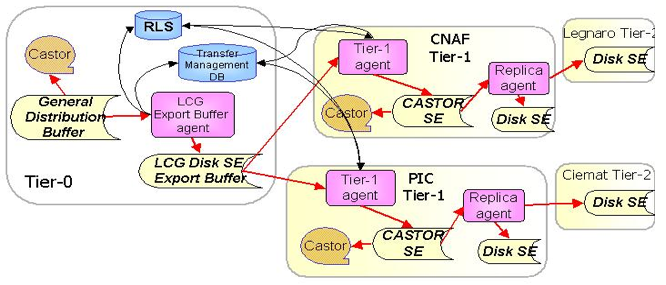
\includegraphics[width=0.95\linewidth]{gross/data_transfer}
  \caption{The DC04 data distribution system.~\cite{Fanfani:2004gh}
  \label{fig:data_transfer}}
\end{figure}

When preparing analysis jobs data discovery was handled through the RLS. Queries were performed with the POOL file catalogue commands. The list of LFN's returned were then listed in the analysis job JDL. Upon receipt of the job the RB looked at the list of LFN's and used the RLS to find sites that held replicas of the required files. The RB then submitted the job to a site within the list.

\subsection{BOSS}
CMS job tracking and submission at this time was handled by BOSS (Batch Object Submission System)~\cite{citeulike:342741}. BOSS was initially developed as a tool for MC production activities at CMS sites and provided a uniform interface to a variety of batch schedulers. It had no CMS specific concepts and thus required directing by a CMS specific application. For production this was McRunJob~\cite{citeulike:867593} but no similar tool existed for analysis. McRunJob created CMS production jobs and used BOSS for job submission and tracking. The advantages of this were that McRunJob could concentrate on CMS-specific functionality (in particular interfacing with the CMS MC production database, RefDB) with BOSS responsible for all common job actions, such as submission and tracking.

BOSS was not a batch scheduler (the workflow is shown in Figure~\ref{fig:boss_Workflow}) and relied on an underlying implementation interfaced via a plugin mechanism. Each batch scheduler was registered to the BOSS system along with a variety of simple wrapper scripts designed to perform standard job actions (submit, query etc.). These were saved to the database with no changes to the core code. When a user requested that BOSS interact with a particular scheduler, the script for the desired action was retrieved and executed. This enabled BOSS to present a uniform interface to multiple schedulers.

\begin{figure}[tbp]
  \centering
  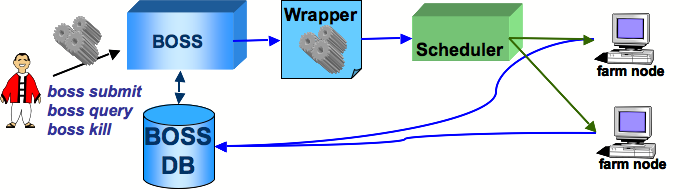
\includegraphics[width=0.95\linewidth]{gross/boss_workflow}
  \caption{The basic BOSS workflow.~\cite{citeulike:342741}
  \label{fig:boss_Workflow}}
\end{figure}

For persistency BOSS used a MySQL database, which was used to store configuration options and job details. Persistent job information stored to the database included details given during job creation such as executable name and input and output files. Once submitted a job returned monitoring information directly to the database. 
%where it was available to the user via the BOSS command line client. 

BOSS also allowed the user to specify the type of executable in the job, called ``job type'', to activate customised monitoring. By registering a job type a user could specify values that were monitored in the application's standard input, output and error streams. This monitoring was performed by a set of scripts, with one for each of the streams that required monitoring. To register a job type the user had to specify a schema that listed the variables to monitor and the set of scripts responsible for monitoring the streams and returning the correct values. For each job type a new table was created in the database with a separate column for each parameter. Each job was represented by a single row and only the last value in each category was retained. When a user specified the job type the relevant scripts were retrieved from the database and sent with the job. This customised monitoring had been used within CMS previously to, for example, record the current event number and allow the job's progress to be monitored. 

User interaction with BOSS was via a Command Line Interface (CLI) or API. The API was a basic C++ API that accepted the same options as the CLI. Simple jobs could be defined by options to the CLI (or API), e.g.. executable name, type and any arguments, while a more complicated job could be described in a Job Description Language (JDL) file. The JDL file was written in the same Classified Advertisement (ClassAd)~\cite{citeulike:835507} syntax as the LCG JDL file. 

Job creation and submission could be combined in a single step or split into two distinct operations. When a job was created BOSS processed the ClassAd file (if used), performed basic checks and saved it to the database. The job was then ready to be submitted. Upon job submission BOSS retrieved the relevant job information from the database and created various submission files. These consisted of files the user requested be sent with the job, the executable and various BOSS programs and files. The BOSS files sent included a job specification file, the monitoring scripts (optional), a program responsible for sending monitoring information back to the database (dbUpdator) and the main BOSS job wrapper (jobExecutor). 

Once the job started the jobExecutor took responsibility for starting the monitoring, running the user's executable and performing cleanup actions. The jobExecutor wrote a log file (journal file) containing a complete log of the job's activity, including general details (start time, execution host, etc.) as well as the information provided by the monitoring scripts. The dbUpdator monitored the journal file and relayed any new information to the database. 

By using the BOSS client the user could query the status of their job. BOSS would first look into the database and, if it was unable to determine the status from this (because for example the job had been submitted but no output had been retrieved) it would query the scheduler.  

When the job finished the output was returned to the user. The output was either saved to a shared filesystem if submitted to a local scheduler or saved to the RB in the case of LCG submission. To obtain output in the LCG case a separate command had to be run. In both cases the output files included the output requested by the user as well as the journal file and the standard output and error. If the dbUpdator was unable to contact the database during execution (generally due to a firewall) then a command could be run that parsed the journal file and populated the database.

%%%%%
%BOSS architecture C++ etc...
%Monitoring need db access. 
%POOL/RLS or in grid chapter?
%API
%May need to expand later - more details when talking about BOSS version 4.
%%%%%

%\section{Overview}
%GROSS was created to provide a reliable method for submitting ORCA jobs to the experiments worldwide resources, for both DC04 and end user analysis. GROSS was designed to handle all the major operations that physicists require when submitting large analysis tasks i.e. once they have written their analysis code and need to run over large amounts of data. GROSS took a users analysis task, split the task into many smaller independent jobs, submitted the jobs to a batch system, monitored them and handled any output files.

%The aim of GROSS was to allow users to submit their analysis jobs to the experiments worldwide resources via the grid. However before DC04 there was virtually no (possibly none at all) user analysis conducted over the grid as there was no policy for distributing event data to the sites. For most analyses both code development and running jobs were carried out at CERN. To increase the chances of users adopting GROSS it was decided that GROSS be able to submit to both grid and local resources.

% In order to run the users analysis as quickly and efficiently as possible the analysis task would be split into many smaller jobs. Each accessing a small subset of the total dataset. This allows for jobs to run at multiple sites, depending on load, and for individual sites to host partial datasets and still be utilised. 

\section{The GROSS design Process}
Before work on GROSS began a full design process was completed. The first step was to determine what functionality and features were required from such a tool. Prior to starting this work an LCG report titled ``Common use cases for a HEP common application layer for analysis'' (HEPCALL II)~\cite{LHC-SC2-20-2002} was published. This document looked at the various types of analyses that would be conducted at the LHC and what software would be needed to facilitate them. Differing scopes of analysis were studied ranging from end user analysis to large-scale managed analyses. Various levels of interactivity were also investigated ranging from fully interactive through to pure batch work.

\begin{figure}[tbp]
  \centering
  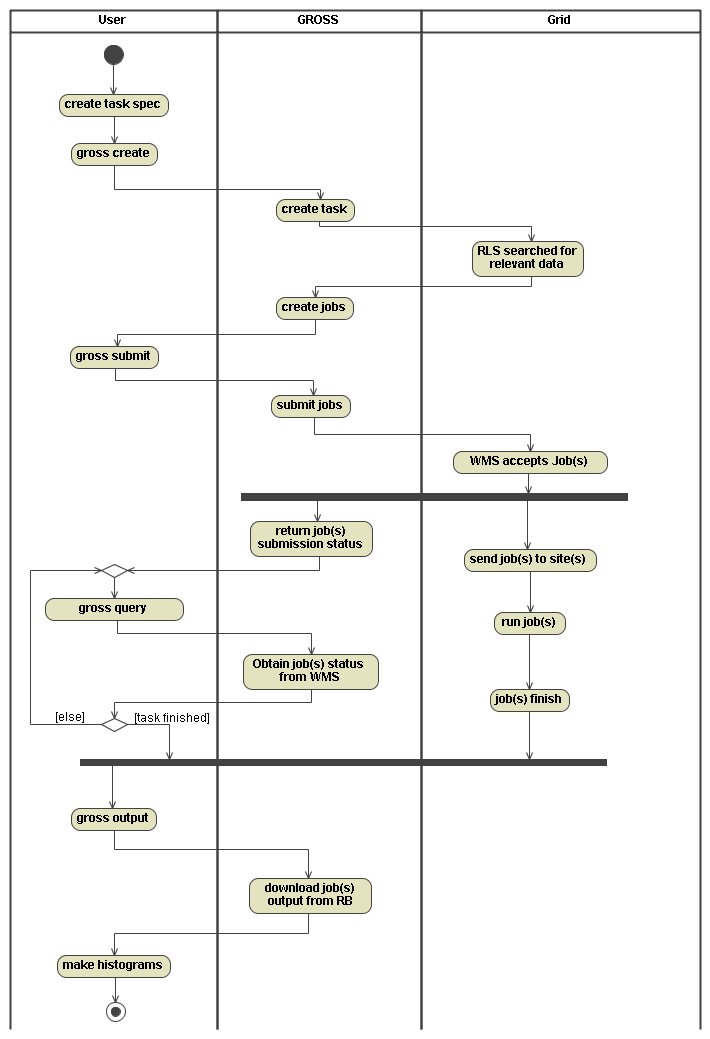
\includegraphics[width=0.95\linewidth]{gross/Overall_Workflow}
  \caption{An activity diagram showing a GROSS workflow consisting of task creation, submission and output retrieval. The User swimlane shows the users actions and the GROSS commands used. The GROSS and Grid swimlanes show the resulting actions of both entities. Note that in this case no output is downloaded until all jobs have competed but this is not compulsory. Output from a job is available for download as soon as the job is finished.
  \label{fig:Overall_Workflow}}
\end{figure}

The end user analyses described in the document included the non-organised analysis r$\acute{e}$gime, where physicists perform un-coordinated work and require as much assistance as possible from the analysis system. The functionality for such a system included file access, job submission and robust provenance mechanisms. The starting point for such an analysis was a query requiring data that met certain criteria (both in terms of data quality and physics attributes), with the user not knowing where the data was located or how to access it. It was also possible that the user had modified parts of the experiments standard analysis code especially for their analysis. The need for logging and provenance information was emphasised with the example of a user attempting to determine where and when certain jobs ran in order to verify their results.

The HEPCAL II document included various models of analyses with varying levels of involvement by the grid WMS in operations such as data discovery and task splitting. The LCG/EGGE did not provide such high levels of functionality and together with the requirement for GROSS to be able to use non-grid resources resulted in GROSS being developed along the lines of the ``No special support by WMS'' model. This resulted in GROSS performing all data discovery, task splitting and job preparation. The WMS treated jobs as simple independent jobs with only a list of site and input data requirements, all features provided by the LCG.

BOSS was a named example of an application with an intermediate level of interactivity where the user had no direct control but did have the ability to monitor closely the process. As GROSS was designed to be used with fully developed analyses interactive control was not required.

From the HEPCAL II description of non-interactive end user analysis with an analysis system designed to work with no special support from the WMS a GROSS use case document was produced. GROSS user requirements were then derived from this document.

The main use case developed for GROSS is illustrated in Figure~\ref{fig:Overall_Workflow}. This workflow described an end user wishing to submit an analysis task and obtain output files. The user had to provide information including ORCA executable, version, configuration file, output file names and the physics data selection query. GROSS would then contact the physics catalogue to discover the list of matching datasets and files. From this GROSS would optionally split the task into multiple jobs, each accessing a subset of the requested data. The task and its sub-jobs would be saved and a numeric identifier (id) returned to the user. With this id the user could then submit the task. Each job was submitted with full monitoring and tracking. At the end of a job the output files would be copied to an SE or brought back with the output sandbox. By running a separate command the user could retrieve the output sandboxes for all jobs in a task.

By the time of DC04 it had become clear that there would be no physics metadata catalogue capable of accepting physics queries and returning a list of matching data. GROSS therefore required the user to specify the requested dataset name when creating the task. If, at a later time, such a physics database was implemented the structure of GROSS would easily allow its use.

Existing tools were utilised whenever possible, minimising duplication of effort and reducing development time. BOSS was used for job tracking, monitoring and submission. Basing GROSS on BOSS allowed GROSS to take advantage of the extensive bookkeeping and job submission features provided within BOSS. GROSS provided the user interface and functionality specific to CMS analysis. 
%GROSS needed a way to contact the RLS and store the returned file list. ORCA required such a list in a POOL file catalogue, therefore it was decided to use this for GROSSs internal file catalogue as well.

\section{Architecture}
One of the main design requirements for GROSS was that it be as modular and flexible as possible. Figure~\ref{fig:Orca_Overview} shows the main GROSS functions and how they relate with external entities. Internally the different components interacted through well-defined interfaces that isolated the rest of GROSS from any component changes. During development the POOL file catalogue API underwent a number revisions but the structure of GROSS restricted the impact of these changes to one component.

GROSS was written in fully object-oriented C++ and utilised design patterns where appropriate. Design patterns are general repeatable solutions to commonly occurring problems within computer science~\cite{citeulike:115158}. 

\begin{figure}[!tbp]
  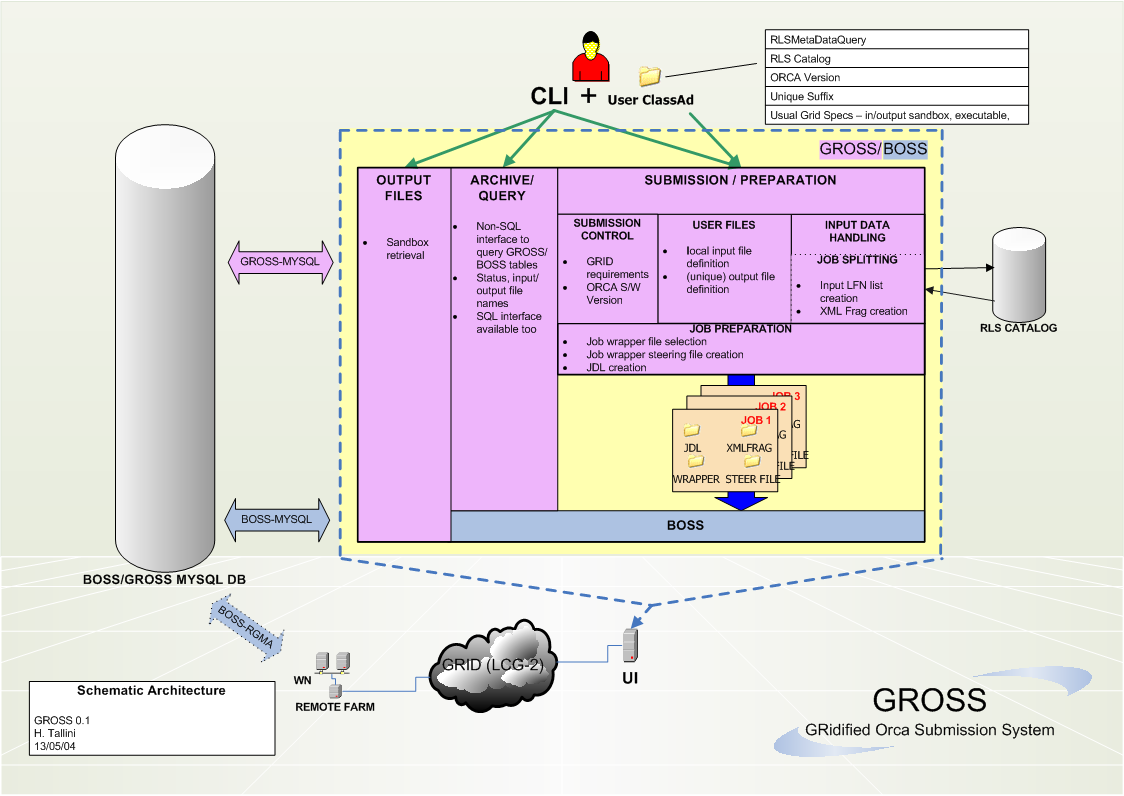
\includegraphics[width=1.5\linewidth,angle=90]{gross/GROSS_Overview_RLS}
  \caption{The main features of GROSS and their relation with external entities.~\cite{CHEP04_TALLINI}
  \label{fig:Orca_Overview}}
\end{figure}

Despite designing GROSS with the primary purpose of creating and submitting ORCA analysis jobs it was decided that GROSS should also be capable of submitting any type of application. Any application-specific functionality had to be part of a modular system. This allowed the future possibility of handling different types of CMS applications, e.g. Monte Carlo production and fast simulation. This was achieved by use of the ``Abstract Factory'' design pattern~\cite{citeulike:115158}, which provides a mechanism for instantiating a family of classes in a uniform and consistent manner. A different family was needed for each supported application (called task types by GROSS). The family provided functionality suited to the particular application including task splitting and submission file preparation.

As BOSS masked the differences between schedulers it had been the original aim that GROSS would remain independent of any scheduler choice, leaving the user free to choose at the time of task submission. However, the large differences in both the execution environment and data access model between grid and non-grid resources made complicated this. A different task type therefore had to be used for ORCA jobs submitted to the grid compared to jobs submitted to a local scheduler. These differences may have been hidden by a sufficiently high abstraction, however this would result in such widely varying requirements for the two cases so as to make it impractical. It was decided that the benefit to the user was outweighed by the development work required, as generally users know if they are submitting to local or remote resources.

The family responsible for ORCA grid jobs is shown in Figure~\ref{fig:OrcaG_Factory}. On the left is the abstract factory that is responsible for instantiating the required classes. When creating a task the type was specified on the command line and the relevant factory implementation instantiated all classes in the family. The task type was saved to the database along with the task so that correct classes could be correctly instantiated in further operations. The family was composed of classes responsible for the task, the jobs, wrapper steering file and JDL. There were two concrete classes responsible for tasks and jobs, one responsible for creating the object from the users specification and the other for retrieving information from the database.

\begin{figure}[!tbp]
  \centering
  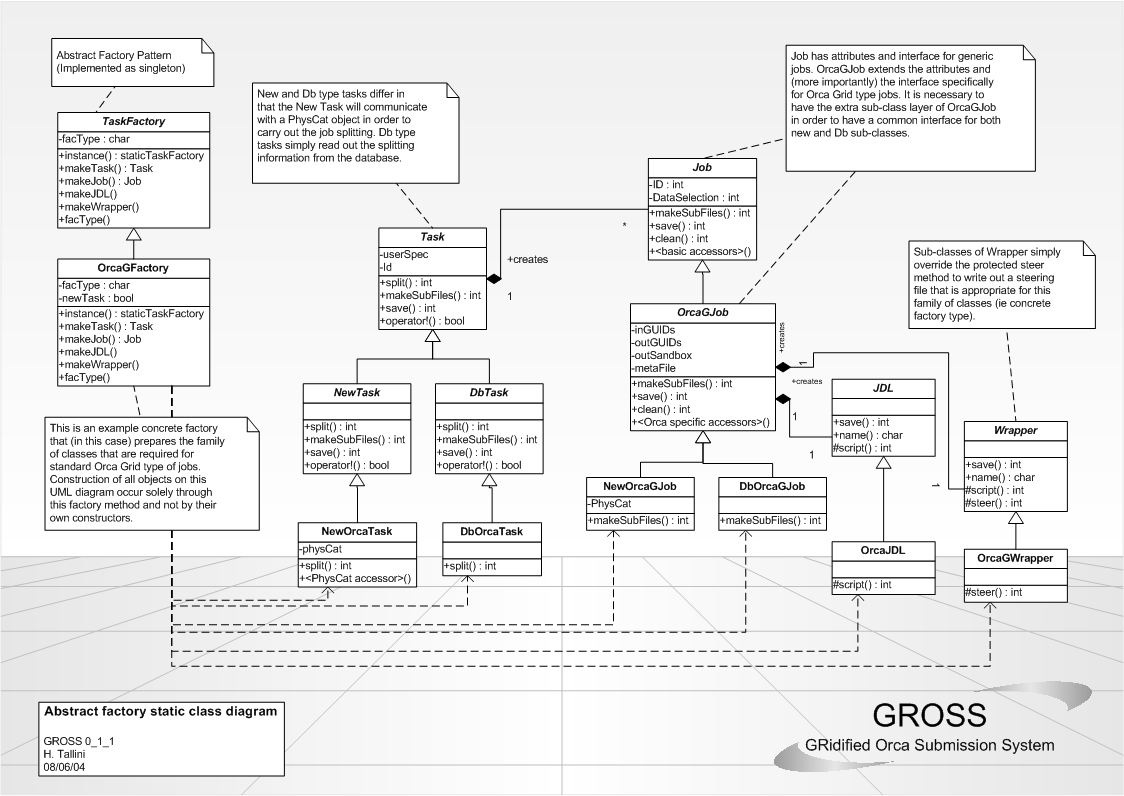
\includegraphics[width=1.4\linewidth,angle=90]{gross/GROSS_UML}\\[1mm]
  \caption{Class diagram showing the abstract factory. ``OrcaG'' refers to the classes responsible for ORCA tasks that are submitted to LCG.~\cite{citeulike:878837}
  \label{fig:OrcaG_Factory}}
\end{figure}

%Database schema - i.e same as BOSS but with a few extra tables.

As GROSS was closely coupled with BOSS it was decided to distribute them together. A user only needed one package and both were installed and configured simultaneously.

As in BOSS it was decided to store all GROSS task information into a database. As most job information was stored into the BOSS database only a few extra tables were required. Thus it was decided to add the GROSS tables to the BOSS database. GROSS access to this database was handled through a singleton~\cite{citeulike:115158}. A singleton is a class that can only be instantiated once, resulting in only one database connection for the whole session. Database calls from all GROSS classes were routed through this object to minimise the database load.

\section{Functionality and interface}
The user interacted with GROSS through a command line client. Options were passed on the command line with the task specification passed via a file (the task specification file). As both BOSS and LCG used ClassAds for their configuration information it was decided to utilise these in GROSS. This allowed GROSS to take advantage of a mature parser library and gave the user a familiar configuration syntax. An added advantage was that unknown fields in the configuration file could be passed down to BOSS, where they might be understood, or, if not, down further to the scheduler. This provided a mechanism for users to provide configuration options direct to the LCG scheduler.

%The GROSS command line took various options depending on whether the user wished to create, submit or monitor a task. All Operations could be performed on a whole task or on a range of jobs within a task. All commands accepted standard parameters that modified the output logging verbosity and BOSS configuration location from their defaults.

\subsection{Task Creation}
%%%%%
%During GROSS's design phase it had been assumed that CMS would have a physcis metadata catalogue that would return data (either dataset or files) that matched a physics query. However by the time of DC04 this catalogue did not exist. Thus a user had to know the name of the dataset they wished to analyse.
%%%%%

Task creation required command line options including task type and the specification file. This file listed all information needed to create the task including the executable file, paths to any libraries required by the application, ORCA version, ORCA configuration file path, the dataset name and output file name. As well as a unique id each task had the option of having a user-defined name associated with it. This was appended to output filenames to aid recognition.

%During task creation the POOL catalogue functionality was used to confirm that the dataset existed and perform the task splitting. Each sub job was configured with the correct data selection, input and output data files. Submission files were generated at this point to allow the user the option of inspecting them before submission. All necessary information was saved to the database, so on subsequent actions the entire task and all jobs could be recreated without repeating the data discovery or task splitting.

\subsection{Input data handling}
At the time of DC04 the expected minimum necessary information required for data discovery was a dataset name. From this GROSS had to be able to discover all data files in the dataset. To allow refinement of this, it was also possible for a user to reduce the scope of the analysis with a further query on the RLS metadata, i.e. on the run number.
%GROSS required an interface to the POOL API that presented all the necessary functionality in a simple and appropriate form.

The ability of the POOL file catalogue to use multiple backend technologies allowed a user to switch between the official CMS RLS and a private POOL file catalogue by changing the file catalogue contact string in the task specification file.

POOL had many dependencies including SEAL~\cite{SEAL} (another LCG project), XML (if used with XML catalogues), MySQL (if used with MySQL catalogues) and BOOST~\cite{BOOST} (a set of C++ libraries). GROSS therefore shared these dependencies. These dependancies would normally have been unacceptable but it was assumed that ORCA, which also required POOL, would be installed to allow the user to develop their analysis. 

Due to the predicted load from the whole collaboration it was decided to reduce the number of queries to the RLS originating from GROSS as much as possible. To accomplish this GROSS implemented a local cache of the relevant information in the RLS. The POOL API provided functionality to extract information from one catalogue and store it in another. Thus the first file catalogue operation performed by GROSS queried the RLS for all information belonging to a dataset and saved this information to a local XML catalogue. All further file catalogue queries were performed on this local copy that, as well as reducing load on the RLS, also improved performance.

%To perform the file catalogue export first a local file catalogue with the same schema as the original had to be created. This involved contacting the existing catalogue, extracting the metadata schema and creating a new local catalogue with the same metadata schema. Then the source catalogue was queried for the owner/dataset pair given by the user and the results saved to the destination catalogue.

One major limitation of the POOL file catalogue API was a lack of ``OR'' logic in query terms; query terms could only be joined with ``AND'' logic or wildcards. GROSS required this functionality for the users optional metadata query, which typically involved queries containing a list of run numbers. To implement this the GROSS POOL interface contained functionality that parsed all query strings for the ``OR'' token. If found the query was split at this point. Each query was then executed separately with the final result set formed from the sum of all partial result sets. Thus, from the user's perspective, ``OR'' functionality was natively supported.

%GROSS made queries of LFN, PFN and run number results from arbitrary complex search queries. The LFN and PFN methods simply queried the catalogue, cycled through the appropriate file name container provided by the API, aggregated the results and returned them. The method that returned the run numbers for the files returned by a query - cycled through a metadata container, provided by the API, searched for the run field and returned a numerically sorted, and unique, list of results to the caller.

%exceptions

\begin{figure}[!tbp]
  \centering
  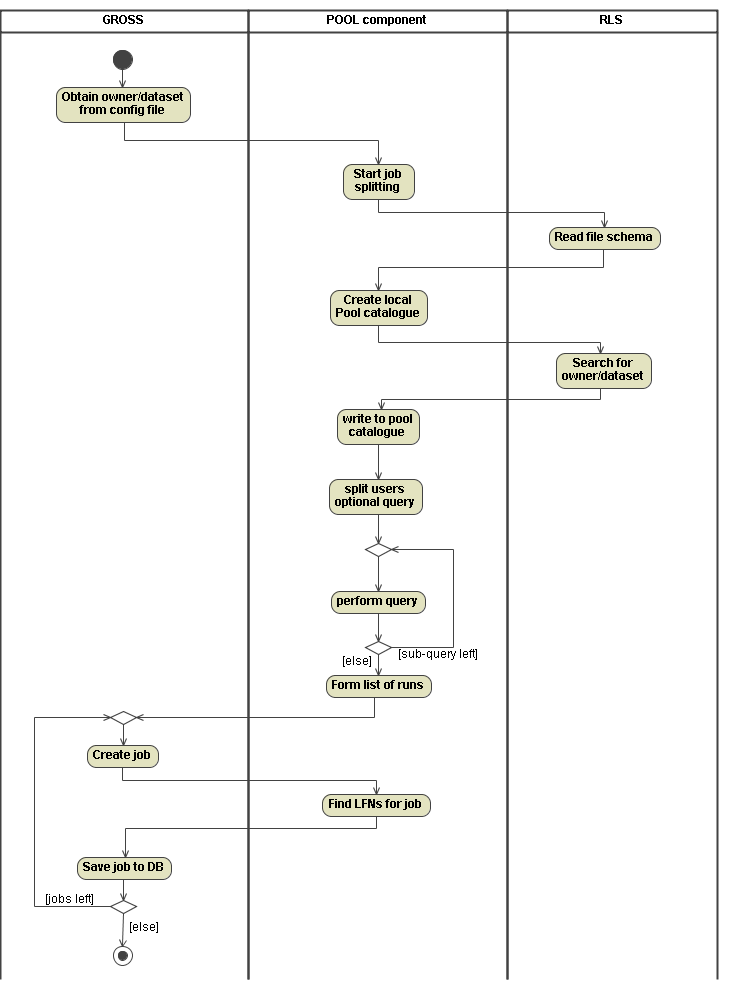
\includegraphics[width=1.\linewidth]{gross/Job_splitting}\\[1mm]
  \caption{Activity diagram showing the task splitting workflow. 
  \label{fig:task_splitting}}
\end{figure}

\subsection{Task splitting}
Each CMS Monte Carlo production job generated a separate run of data, hence it seemed logical to split the analysis task in the same way. This allowed maximum flexibility for job submission. Each job required the minimum number of files for a given number of events and each file was needed by only one job, so allowing each job within a task to be sent to a different site. This splitting was only appropriate for an analysis case where the majority of events were fully analysed, as was the case with most CMS analyses in 2004. This would not be the case with real data where not every event in a dataset would prove interesting to every analysis. Hence this strategy was appropriate for Monte Carlo analyses but not for real data.

The task splitting workflow is illustrated in Figure~\ref{fig:task_splitting}. Once the local file catalogue containing all files within the dataset had been created, a list of runs was produced subject to the optional user-provided metadata query. This list was then used to create the sub-jobs. Once jobs had been configured with their run number they could then obtain a list of their input data files by querying for all of the LFN's for their run. The archive file containing the metadata also had to be discovered and added to the list of input files for each job.

%The number of runs analysed by a job was user configurable as the time taken for anlyses varied greatly. later

Each job was configured with the correct data selection, input and output data files. Files generated during configuration included a POOL XML fragment listing the input data, a JDL file for the RB and a configuration file for the wrapper script that ran the appropriate workflow on the worker node. All information was saved to the database, so in subsequent actions the entire task and all jobs could be recreated without repeating the data discovery or task splitting.

%The user analysis application was run by a wrapper script which also set up the CMS environment and handled output files at the end of the job. Each job required a configuration file to steer the job wrapper, a POOL XML file catalogue fragment listing the input data files and a JDL file describing the job to be given to BOSS. The steering file contained all the information necessary for running the job, i.e. the ORCA version and executable to run. The JDL file for each job contained the list of required input data and the required ORCA version, to allow the RB to steer the job to the correct location.

%Once a task had been split the constituent jobs were saved to the database. All relevant information was saved including the POOL XML fragment - therefore at submission no information had to be re-calculated.

%%%%%
%Step before submission - files etc...
%ave to database
%split acording to directive  - 1 or many runs per job
%job - list of files needed
%steering file
%Pool XML Fragment - only files job needs + meta
%metadata
%out files
%prepare tar - wrapper, BOSS, etc..
%register to BOSS
%unique Suffix i.e. task name
%%%%%

\subsection{Task submission}
To submit a task the user provided the task id and the desired scheduler. GROSS then retrieved the task and sub-jobs and prepared the submission files. These files included the user-defined files, ORCA configuration file, user's executable, user libraries, wrapper script and the wrapper script steering file. Each job was submitted to BOSS with the GROSS job type to activate the specialised monitoring. After submission each job record in the GROSS database was updated to point to the BOSS job record, which contained information such as scheduler id and status.

%bit more about scheduler stuff temp file creation? BOSS etc? BOSS job archive dbUpdator

\subsection{ORCA wrapper script}
%workflow when landing on worker node
%
Before ORCA could be run a number of steps had to be taken: the CMS environment needed to be set, input files  located, the user's executable and libraries prepared and many other operations. In order to perform these tasks a wrapper script was necessary. The script had to be lightweight, fast and capable of running on many different types of operating system and architecture. This script was implemented as a shell script that provided a capable but lightweight solution.

%This script was implemented as a shell script, this was chosen as a capable but lightweight solution. The LCG utilities that provided functionality for RLS and file operations were also required, however these were available by default on LCG worker nodes. An installed version of ORCA complete with POOL file catalogue commands was also needed. 

%A way to extract the metadata from the zip archive was required, however the usual program for this unzip (or gunzip) was not always available on worker nodes. This was solved by using the program responsible for java archives which was also able to extract files from zip archives, and as the LCG tools required java this was always present. 

Once a job began on a worker node a process similar to the job preparation step, but in reverse, was run. The local scheduler system started the BOSS jobExecutor, which had to set its own environment before starting the GROSS wrapper. The GROSS wrapper script then set the local CMS environment before starting ORCA. 
%By the time BOSS started the GROSS wrapper script the monitoring had Been activated and all files brought by BOSS were available. 
%The wrapper script printed checkpointing, information and error messages which were recognised by the customised BOSS monitoring scripts. 

%The standard output and error of the wrapper script were continually monitored by BOSS. The wrapper script provided mechanisms for printing out checkpointing, information, warning and error messages. These messages were available to be picked up by BOSS's monitoring. These messages were printed out regularly by the script so the user could follow the scripts progress. 

The wrapper script obtained its configuration information from the steering file. If the script was unable to locate this file the wrapper aborted. Once located this file was parsed and its contents (key-value pairs) placed into variables within the script. After this a check was performed to confirm that certain critical variables were defined. These variables included executable name, ORCA version etc.

The CMS software area was located using an LCG-defined environment variable. In this area was a script, created by the CMS software installation, that set up the CMS environment. After the CMS environment was available the ORCA environment was required. The GROSS wrapper script took the version of ORCA requested, checked its availability and sourced its environment.

%Next all the required files, both local and grid, had to be checked and properly handled. A temporary area to run ORCA in had been created so the files brought with GROSS had to be moved there. These files included the ORCA configuration file, POOL XML fragment and any other files requested by the user. An environment variable was created pointing at the POOL XML fragment that had the effect of making all subsequent POOL file catalogue commands use this catalogue. 

\begin{figure}[!tb]
  \centering
  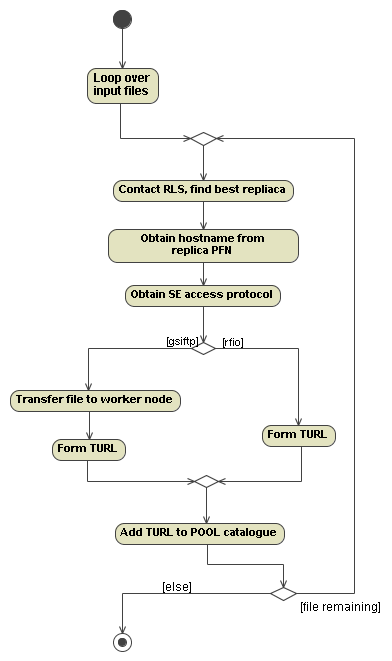
\includegraphics[width=0.55\linewidth]{gross/Wrapper_FileAccess}
  \caption{Activity diagram showing wrapper script workflow for locating input files. The deprecated direct file access protocol is not shown.
  \label{fig:Wrapper_fileAccess}}
\end{figure}

Next the input data files had to be located. It was LCG policy to send jobs only to sites that hosted all of the required files on their SE. The LCG SE supported three file access protocols: direct file access, RFIO and GSIFTP. Direct file access assumed that files were available from the worker node filesystem. This mechanism was deprecated due to scalability issues and was dropped from later LCG releases. RFIO was a widely supported file access mechanism within HEP that allowed files stored on a server to be accessed from remote clients and was the recommended access method. It required that applications support the protocol, which most HEP applications at the time did. The GSIFTP protocol was the standard mechanism for transferring files between LCG SE's. It was an FTP implementation that utilised the LCG security model (X509 certificates). ORCA could not use GSIFTP for file access and so files first had to be downloaded to the local filesystem. This resulted in the use of unnecessary bandwidth between the SE and WN and the need for temporary disk space on the worker node. By definition an LCG SE had to support the GSIFTP protocol whereas the others were optional. This meant that the script had to discover the access protocols provided by the SE and take appropriate action.

A site may have had more than one SE hence, for each file, the hosting SE had to be found and the supported protocols discovered. The workflow is illustrated in Figure~\ref{fig:Wrapper_fileAccess}. This information could be obtained from the brokerInfo file~\cite{citeulike:835506}, a file created by the RB on job matching and sent with the job, containing information about each SE at the site that hosted input data, including supported protocols. Thus for each file the script obtained the location of the closest replica from the RLS including the hosting SE. Using the information in the brokerInfo file the SE's list of supported access protocols was discovered. The scripts then applied rules to find the correct access mechanisms, trying in the order RFIO, file and then GSIFTP. Once the access protocol had been discovered the script had to form a correct contact string, possibly copy the file locally (in the case of GSIFTP) and update the XML POOL fragment, sent with the job, with the new contact string. 
%For each LFN POOL file catalogues allow multiple contact strings and when asked for a contact string provide one of them at random. Therefore all existing contact strings for a LFN were overwritten with the correct value.

Even if the metadata archive was available over RFIO it was copied to the local disk to allow the metadata files to be extracted. 
%. This was because the program used to extract files from the archive could not use the RFIO protocol.
The metadata archive contained several POOL XML fragments describing the metadata files. Once extracted the script merged these with the POOL fragment from GROSS and processed each of the files, setting the contact strings to point to the newly-extracted files. The metadata was virgin, therefore ORCA could not read it and go straight to an event within a data file. A program distributed with ORCA first had to be run on the event data files to find the event collection identifier, which was then added to the ORCA configuration file to allow ORCA to access the events.

Before running the user's executable a check was made to ensure that all of the required libraries were available. If libraries were missing the script exited with an error. ORCA was capable of providing useful output but still exiting with a non zero exit code, in this case the script continued but recorded the exit code for later use. Once an output file was found, it had the optional task name appended and was either saved to an SE and registered with the RLS or returned via the LCG output sandbox. Figure~\ref{fig:Wrapper_OutputFilesRLS} shows the workflow for registering output files with the RLS. Files were saved to an LCG SE local to the the site and registered with the same LFN as their filename.

\begin{figure}[!tbp]
  \centering
  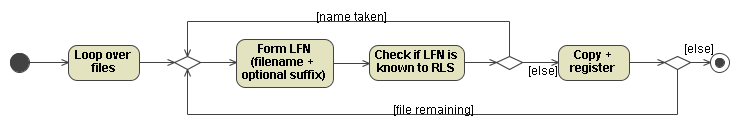
\includegraphics[width=1\linewidth]{gross/Wrapper_OutputFilesRLS}
  \caption{Activity diagram showing wrapper script workflow for registering output files with the RLS. If an LFN already existed GROSS did not overwrite it. It was the user's responsibility to ensure that output from previous tasks with the same optional suffix no longer existed.
  \label{fig:Wrapper_OutputFilesRLS}}
\end{figure}

Finally the script removed all files it had created and exited with the same error code as that of the user's ORCA executable. BOSS recorded the exit code (and various statistics), collected all of the output files and exited. 

\subsection{Querying and output retrieval}
Once the task had been submitted the status of its constituent job's could be queried. If GROSS was unsure of a jobs status, i.e. the job had been submitted but not retrieved, GROSS queried BOSS. BOSS then queried the database for the job state, and, if this could not be determined, the scheduler was queried. 

All GROSS jobs were submitted to BOSS as a member of the GROSS job type. This job type was registered during the GROSS installation and registered monitoring scripts designed to monitor the wrapper error and information messages. If the running job was able to contact the GROSS database then these messages were continually relayed to the database. The database held the last message in each category for each job. This information was accessible from the GROSS command line.

Once a job had finished the output could be retrieved. When a user requested that a task's output be retrieved, GROSS located the jobs that had completed and asked BOSS to retrieve their output files. If the output was retrieved successfully the GROSS database was updated. By using the GROSS client the user could later determine where a particular task's output had been saved.

\subsection{Local farm submission}
Job preparation and execution on a local batch farm required significantly different steps from a grid submission, requiring the introduction of another task type. This task type assumed that the user had a POOL file catalogue containing a locally available dataset. This may have been the RLS in the case where a user wished to bypass the LCG and submit directly to local resources. This only worked in the case where the registered PFNs were also the file contact string, which was the case at CERN but not at LCG sites in general. 
%Though this worked only where the pfns's registered to the RLS were the contact strings for the local site, this was not the case for files saved to LCG SE's but was for CERN. 
The difference in data discovery between the two task types was that the local type resolved file contact strings at creation time whereas grid jobs determined this at runtime given the site at which they ran.

The local version of the wrapper script provided similar functionality to the grid script. File access was simplified as it was assumed that the POOL fragment already had correct contact strings. Not all local batch systems supported input or output file handling, therefore all files had to be available on a shared filesystem. At the end of a job the output was copied back to another location on the shared filesystem specified when the task was created. The GROSS output retrieval step was not necessary.

\section{Performance and useability}
Unfortunately GROSS development progressed more slowly than originally envisaged and DC04 had already begun by the time it was released. Due to the amount of data to be analysed an automated procedure using custom software agents had been developed (Figure~\ref{fig:dc04_analysis}). These agents were tightly coupled with the transfer system. Once files appeared at CERN and were registered in the RLS they were transferred to a remote site, the replica registered and an analysis job sent via LCG. The executables and libraries were sent together with the job and the output was saved to an SE and registered to the RLS. Job submission and monitoring were provided by BOSS. In the last two weeks of DC04 15,000 jobs were sent, with a grid efficiency (i.e. the efficiency for a job to be executed at a site irrespective of the success of the application) of 90-95\% and a latency of 20 minutes between files appearing at CERN and their remote analysis~\cite{citeulike:621630, Fanfani:2004gh}.

\begin{figure}[tbp]
  \centering
  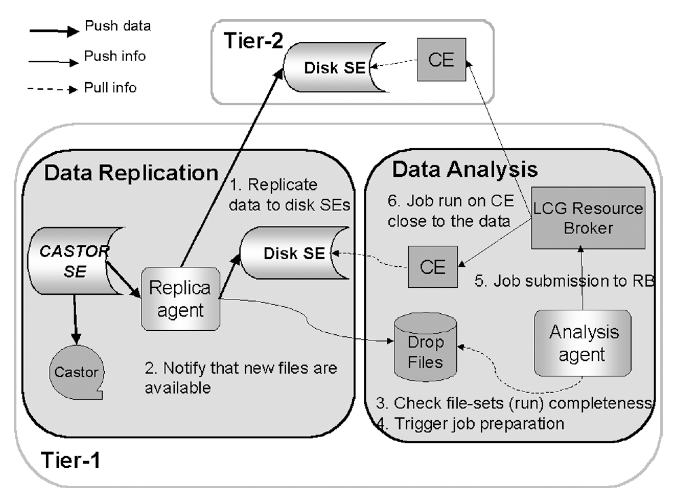
\includegraphics[width=0.85\linewidth]{gross/data_analysis}
  \caption{DC04 real time analysis chain.~\cite{citeulike:621630}
  \label{fig:dc04_analysis}}
\end{figure}

During this time the developers evaluated, tested and made several enhancements and bug fixes to GROSS. While all functionality worked as intended the performance was worse than expected. Specifically the data discovery step was found to be unacceptably slow, which was traced to poor performance of the RLS. 

The RLS consisted of several components: the Local Replica Catalog (LRC), which maintained the list of replicas at a site, the Replica Location Index (RLI), which indexed multiple LRC's and the Replica Metadata Catalog (RMC), which held file metadata~\cite{citeulike:623288}. Within LCG the RLS had only been implemented as a single LRC (and RMC) per experiment instead of per site as it had been designed. The LRC had been evaluated with inserts, deletes and queries on LFN's. These tests and experience during DC04 showed acceptable performance~\cite{citeulike:623294, baud2004eld}. However, metadata tests had only involved inserts and deletes. Once the system was queried for all files meeting certain criteria it became apparent that performance was unacceptable~\cite{citeulike:623294, baud2004eld}. Queries for all files belonging to an average CMS dataset ($~\sim$1000 runs), as required by GROSS, took 2--3 hours to complete~\cite{citeulike:623294}.

The real time analysis was only concerned with LFNs and so was able to avoid the poor performance of the RLS with metadata queries. GROSS, however, was based on the premise that the user did not know the files they wished to analyse, only the dataset. One way to improve performance was to use the POOL file catalog commands manually to perform the search of the RLS and to store the results in an XML catalogue. If this was then used with GROSS and multiple tasks were created against the dataset, performance was seen to improve with data discovery taking minutes rather than hours.

%more on usage?

\section{Post DC04 distributed analysis}
%put 0_2_0 here i.e. intermediate metadata, multiple runs ...

After DC04 CMS decided that instead of requiring LCG to optimise the RLS it would eliminate the need for a global file catalogue. Instead a central catalogue would keep a mapping between datasets and sites. Each site would then host its own file catalogue (possibly more than one). In this model the central catalogue would contain significantly less information and be subject to fewer simpler queries, which improved performance. Each site had a web-accessible service, known as a  PubDB, which would return the correct file catalogue(s) for a dataset~\cite{citeulike:623034}. The file catalogue could be any POOL file catalogue and was generally either XML files or a MySQL database. 

The data movement system was re-engineered but still consisted of transfer agents at each site controlled by a central database. The site agents periodically queried the database and discovered any outstanding data requests. The agents downloaded the relevant files and marked the transfers as complete in the database. Only event data was known to the CMS data management system, hence, before the dataset was available for analysis the metadata had to be downloaded in a separate publishing step. Here the virgin metadata was downloaded from CERN and populated. These and the event data files were then added to the local POOL file catalogue(s).

The result of these changes was that jobs no longer needed to carry their own file catalogue or know \emph{apriori} which files were required. It was the responsibility of the site to provide the job with the means to locate all files needed at runtime.

%%%%%\section{New GROSS architecture}
%%%%%
%This change sped up GROSS considerably and reduced the amount of data stored in the database. When the task is created the only data discovery steps needed are to ensure that the dataset exists and that at least one site has a copy. During the time interval between task creation and submission a site status may have changed so the list of hosting sites was formed at submission time.  GROSS contacted the hosting sites to find the contact strings for their file catalogues. The list of sites is then added to the JDL to allow the RB to send the job to the correct site and the list of file catalogues is provided in the steering file for the wrapper script.
%%%%%

In the transition period between the phasing out of the RLS and adoption of the PubDB system an interim solution was used. Full (i.e. non virgin) metadata was made available via the CMS MC production system. Once a dataset had been produced it was copied to CERN, where the metadata was fully populated with information about all event data. These metadata files were then made available from the CMS web server. During the data discovery stage GROSS contacted both the RLS for event files and the CMS webserver for the metadata and a POOL catalogue fragment. These were then both sent with the jobs. This temporary procedure was only needed while the PubDB system was being developed.

\section{CRAB}
Around this time another tool called CRAB (CMS Remote Analysis Builder)~\cite{citeulike:876380}, developed by a group from Italy, was released. This tool was similar to GROSS with only minor differences. During December 2004 a meeting was held in Bologna to decide the future of CMS distributed analysis. At this meeting a comparison of the two applications was carried out. 

CRAB was written in Python and did not utilise BOSS. These choices and the relatively large development team allowed CRAB to develop PubDB support before GROSS. The lack of BOSS integration simplified the installation of the software and eliminated the requirement for a MySQL database but resulted in poor job tracking and logging. There was no central repository where information about all tasks could be found. Each task had its own directory for submission and output files and this directory had to be retained if the user wished to retain knowledge of the task.

CRAB also had other features aimed at simplifying its use. It was integrated with the CMS build system and thus, with the appropriate ORCA environment set, could locate the users executable and all libraries. GROSS, in contrast, required the full path to each to be listed in the configuration file. With CRAB, tasks could be created, submitted and scheduled for automatic file retrieval with a single command. The same workflow in GROSS required at least three separate commands. However, GROSS had a much clearer and more consistent command line.

Overall it was felt that GROSS provided a more uniform interface and better job monitoring and bookkeeping but CRAB was easier to install and provided many features that simplified the analysis process for the user.

As a result of the meeting it was decided that both applications would continue to be developed whilst an evaluation by the CMS physics community was conducted. CRAB would investigate using BOSS to provide job submission and logging and GROSS would adopt the PubDB system and some of the ideas in CRAB aimed at simplifying and automating the analysis process for the user.

\section{New architecture and features}
Until the meeting in Bologna GROSS had been distributed together with BOSS. Many sites, however, already had an installation of BOSS from CMS MC production activities, so it was decided to package GROSS separately.

The change to using the PubDB system required a large change in the architecture of GROSS. Previously each job had known about all input and output files, but this information was no longer necessary. GROSS now relied on a correct POOL file catalogue at the site to contain the requested data. The facility for users to send jobs using their own POOL file catalogue to local resources was still maintained.

Previously, analysis with GROSS had only focused on the Hits data tier, whereas most advanced Monte Carlo analyses required access to both the Hits and the Digis. This required access to data from two owner/datasets and possibly the pile-up dataset also. The PubDB system had been designed to cope with this and for each owner/dataset the central PubDB listed the related owner/datasets. In the task specification file the user could request data tiers related to the the specified owner/dataset. GROSS would then ask the central PubDB catalogue for their entries as well. Sites were not required to host entire datasets, only a continuous range of complete data runs. For each job GROSS required that a site hold the same run in all data tiers, plus the complete pile-up dataset. The ability to access multiple data tiers was only required for analysis of Monte Carlo data.

The move to PubDB improved performance considerably. The data discovery step was now simplified, when the task was created the only data discovery steps needed were to ensure that the dataset existed and that at least one working site had a copy. This was in contrast to the previous situation where every file within the dataset has to be located. The combination of the new system and simpler queries resulted in a considerable performance gain, with data discovery taking approximately 10\,s.

During the interval between task creation and submission the status of the sites may have changed, so the list of sites was formed at submission time. GROSS contacted each hosting site to find the contact strings for the file catalogues. If a site did not respond within a set time it was skipped and GROSS moved to the next site. The list of appropriate sites was added to the JDL to allow the RB to send the job to the correct site and the list of file catalogues was added to the steering file for the wrapper script.

Previously GROSS had split a task into one job per run. However, as the time required for different analyses varied greatly this was modified so that the user could change this. As well as specifying the number of runs to analyse in a job the user could also specify the start and end run numbers if they did not want to analyse all runs within the dataset.

During Autumn 2004 LCG sites began to migrate their operating systems from RedHat Linux 7 to systems compatible with Scientific Linux CERN 3, SLC3~\cite{SLC3} (a RedHat Enterprise 3 derivative~\cite{RHEL}). Applications built on SLC3 could not run on RedHat 7 systems. LCG sites specified their operating system in the information system. If a user wished to run on a certain architecture they could add a ClassAd requirement to the task specification file, which would then be passed to the RB at submission time. To allow access to all sites GROSS provided the option for users to send their source code and have their analysis application built on the worker node. If this was requested the user's code would be built in an ORCA environment on the worker node, with the resulting executable automatically linking with the standard ORCA libraries already present at the site. If any errors were encountered during compilation the job would abort.

%The task querying functionality in GROSS had lower than expected performance. The cause of this was found to be due to the handling of status queries within BOSS's LCG scheduler script. Rather than performing a simple status query on each job, the plugin requested the status of all BOSS jobs submitted via LCG and then searched amongst this list for the status of the particular job. This problem only became evident with time as more and more jobs had been submitted. This was compounded as BOSS had no knowledge of the task structure and therefore queries of a tasks status resulted in a separate status query for each job, each of which queried all jobs submitted via LCG. As GROSS was now packaged separately from BOSS and sites all had their own version's it was not possible to patch the LCG query script. Therefore a temporary fix was introduced to GROSS, it was impossible to speed up BOSS's query so instead the approach was to minimise the number of times the query was run. Oringinally for each job a separate BOSS command was run that returned the status of that job, this was changed to a query that returned the status of all jobs submitted via LCG, these results were then cached locally by GROSS. When the status of the next job in the task was requested GROSS looked in this hash table to check for a match, if found this was returned if not the BOSS query was executed as usual. This sped up the query considerably, especially for large tasks.

During one of the LCG upgrades, limits on the input and output sandbox sizes were introduced. The RB stored these and a number of users were sending and/or retrieving very large files via them. This had the effect of filling up the RB's disk and affecting its performance. The limit imposed on input sandboxes was 10MB. GROSS sent the user's pre-compiled binaries as well as files needed by both GROSS and BOSS. The ClassAd library, which was sent to allow BOSS to read its configuration file, was about 7MB, which, together with the user's executable, easily exceeded this limit. It would have been possible to install the ClassAd library at each site, thus circumventing the restriction. However this would require support for each site along with a versioning mechanism to handle different BOSS versions. Thus it was decided that the BOSS developers should attempt to reduce the size of the libraries required by BOSS. A simpler version of ClassAds, called ClassAdLite, was developed which was only a few hundred kB.

In order to help reduce the output sandbox size the facility to allow files to be saved to a set path on a SE of the user's choice, without being registered with the RLS, was introduced. This was easier for users to use than the RLS as they could see files accumulate on an SE, e.g. their private area on CASTOR at CERN, rather than having to query a remote service.

Originally it was foreseen that automatic output retrieval would be handled by a cron-like entity calling GROSS at regular intervals to download any remaining output files. However, the availability of cron was not guaranteed at every site from which users submitted CMS jobs. An alternative method was chosen that made use of an agent process to periodically run GROSS. If, when the user submitted a task, they requested this functionality the script was started on the UI after submission. This script slept for a user-configurable time, then woke and ran GROSS telling it to retrieve any available output for the task. If no output was available the script would go back to sleep. When GROSS reported that all output had been collected the script would exit and if the script was still active after a user-configurable time limit (by default 2 days) it would exit anyway. This was to prevent it from running forever when a problem prevented retrieval of the output. The script wrote to a log file so that users could follow its progress and see how much output remained. If the user ended the session on that machine the process would continue, as it ignored SIGHUP signals. This feature was not enabled by default due to concerns about users starting large numbers of processes on popular machines. 

Output files were stored in a separate directory for each job under the user-specified area, with the optional user suffix appended to each file. As a result of the task splitting it was not uncommon for a user to have hundreds of small ROOT files in different directories. This made keeping track of files or running ROOT over the files inconvenient. Therefore new functionality was introduced that allowed the user to obtain one root file for a whole task. 

By running a script in the GROSS distribution the user could merge all the ROOT files within a task. It was also possible for the user to merge only the output from a subset of the jobs in the task. This script ran GROSS to discover the location of the output files, and any jobs that had finished but whose output had not been retrieved had their output collected. A search for ROOT files was then carried out and any found were added to the list of files to be merged. ROOT was then run, merging all the input files to create a new ROOT file in the specified location.

With jobs submitted to the LCG it was not uncommon for a number in any given task to suffer transient errors, either within the LCG workload management system or because of the configuration of an individual site. To help with this problem a mechanism for resubmission of failed jobs was added. Using this command GROSS would resubmit any failed jobs in a task, or job range within a task. 

Real time monitoring was improved by modifying the GROSS job type to recognise the standard ORCA event number printout. This allowed users to monitor the current progress of their jobs.

%multiple out files
%gross split run - crab events
%merge with BOSS
%Meeting december ??
%decided 
%  1 step submission
%  laptop - prepare online - simpler?
%  move to pubdb - timeout automate etc...
%  need ancestor datasets
%  scram integration
%  auto retrieve
%  non virgin metadata
%class as lite 
%crab?? what mention?
%scram build

\section{Community Evaluation}
Once most of these changes had been made GROSS was made available to the CMS physics community. GROSS was evaluated by members, including the convenor, of the Higgs PRS (Physics Reconstruction and Selection) analysis group. GROSS was used to perform analysis for $\tau$ jet studies and Higgs searches on Monte Carlo data.

The $\tau$ studies consisted of two areas of activity: jet calibration and HLT studies. The calibration study involved developing a Monte Carlo jet \ET calibration for $\tau$ jets. This was achieved by running over a sample of 100,000 hadronically decaying $\tau$'s and comparing the Monte Carlo and reconstructed jet \ET. An algorithm was then developed in ROOT to relate the two. The HLT $\tau$ jet studies looked at trigger optimisation specifically for the MSSM heavy Higgs decaying to two $\tau$ jets.

Higgs analyses included the channels MSSM $H \rightarrow 2 \tau $ jets, MSSM $H \rightarrow 2 \tau \rightarrow \tau \textrm{jet} + l$, MSSM $H \rightarrow 2 \tau \rightarrow 2l$ and MSSM $H^{+} \rightarrow \tau$. These analyses involved running over both signal and background datasets. Backgrounds included QCD multi-jets, W$ + $jets and Z/$\gamma \rightarrow \tau \tau$. The analysis of signal events required the full analysis of the majority of events. Where the backgrounds were likely to be rejected they were preselected, during generation, to be more likely to pass the analysis cuts. Thus this testing used the majority of the available sample and hence did not represent a realistic indicator of performance with real data. 

In these analyses 4 users created $\sim$220 tasks analysing 22 datasets. A total of 4,381 jobs were submitted to BOSS, of which 4,181 were successfully submitted to a scheduler. Of these 3,134 were submitted to LCG and 1,047 to resources local to CERN. 3,726 jobs finished successfully, representing a success rate of 89.1$\%$ and leaving 455 jobs that exited with errors. These errors generally indicated a problem with the user's code (possibly something that was not apparent during limited use) or a (transient) problem at a site, often with file access. It was not possible to give a detailed breakdown of the various failure modes as the ORCA exit codes did not always correspond to the actual error. Also, any user requested job resubmission would have overwritten the details of the previous job in the database. Thus the 89.1$\%$ success rate represented the rate allowing for re-tries. In total these jobs used over 605 days of computational time.

These statistics were taken from the GROSS/BOSS database. If a running job was unable to contact the database the records may be incomplete. In this case GROSS attempted to correct the situation at the output retrieval stage by running BOSS with the retrieved journal file. This process was not, however, always reliable.

%%%%%%%%%%%%%%%%%%%%%%%%%
%4 users
%13775 jobs
%222 tasks 
%avg 55 jobs per task.
%me - tau calibration, 	bt04_double_tau_hadr, jm03b_qcd_50_80
%slehti MssmA2tau2l	hg03_h2tau_2l_200 hg03_hsm120_mumu hg03_zg80_100_2tau_2l
%Sasha - MssmA2tau2j, 
%        tau HLT 	bt03_mssm_h2tau_jj200 bt03_mssm_h2tau_jj500 bt03_qcd80-120_2tauj jm03b_qcd_50_80
%kinnunen - MssmHighmHchTauJ	hg03_thplus200_tau
%22 datasets
%
%Feedback - merge root files, take all info from db
%           concurrency problems database, 
%           error testing check for edg tools and proxy
%           lsf queue
%           first/last run - easier than meta query (did this apply to pubdb - no)
%           resubmission of failed jobs
%           globus-url-copy out files - not save LFN i.e. to own castor area
%need parent datasets
%prob monitoring - mysql - try to get journal files - not always work          
%%%%%%%%%%%%%%%%%%%%%%%%%

\section{Conclusion}
GROSS met all of the requirements set out in the design phase and was a proof-of-principle tool for distributed analysis within HEP. It proved useful for physicists during work leading up to the writing of the CMS physics TDR~\cite{CMS_TDR_PHYS_vol1}. It allowed a physicist to perform an analysis over large amounts of data distributed between CMS' resources worldwide. The use of GROSS by physicists in their work provided much needed-feedback and allowed the introduction of a large number of bug fixes and new features. 

Compared to CRAB it was felt that GROSS provided better logging and monitoring, implemented through BOSS, but that CRAB was a more lightweight and flexible design. CMS decided that CRAB provided the more appropriate client-facing application, but recognised that GROSS was more robust and through BOSS provided many useful features. Thus it was decided to introduce many of the features GROSS provided, i.e. the task concept and handling, into BOSS, while CRAB would act as a CMS-specific application relying on BOSS to provide the task submission and logging functionality. The BOSS development work is described in the next chapter.


% BOSS v4 section
\chapter{Boss development}
\section{Introduction}
BOSS had been used since 2002 within CMS production~\cite{citeulike:877254} and in DC04 with analysis~\cite{CHEP04_TALLINI, citeulike:876380}. After DC04 it was decided that BOSS would be integrated into both systems to provie generic batch job functionality. The opportunity was taken to re-design BOSS completely to fit this role better, existing functionality was improved and new features introduced~\cite{citeulike:880984}. New features included the concept of a task and the possibility for a job to run more than one application. Improvements were made to the monitoring (removing the direct database connection) and logging (eliminating the requirement for a database server). 

%%%%%
%ituent jobs and allowing a job to run more than one user application (so called job-chainning) in a user defined workflow. Many other improvements and refinements were introduced; improved logging (removing the need for a MySQL database server), improved monitoring (removing the direct database connections from jobs).
%%%%%
\section{Limitations of previous versions}
%. These experiences pinpointed various limitations and possible improvements. Some of the proposed changes implied large scale architectural changes i.e. support for the task concept.

The lack of a task hierarchy required both CMS production and analysis systems to operate BOSS with an ensemble of individual jobs. A separate BOSS invocation was required for each job, with no sharing of information between instances.

The BOSS API did not offer any greater functionality or control than the command line client. The only available operations were the high level command's accepted by the command line, i.e. job creation and submission. To get feedback from the operation the calling application had to parse the commands output. The API was implemented only in C++ and thus was unavailable to the large amounts of CMS software written in other languages. As a consequence both CRAB and the Monte Carlo production system ignored the API and used the command line client.
% It was thus decided to replace this API with one that had much greater functionality and finer grained control. This API would also be implemented in multiple languages widening its availability.

%  required the calling program to place the same options as would have been passed on the command line into a string and simply pass these to the API. The API provided no extra functionality or control than the command line. Only a C++ API existed thus it was only convenient for other C++ programs to call. Thus there was very little benefit to using the API. It was decided to replace this with an API which had much more functionality and could be implemented in many languages.

Installation was complicated by the requirement for a MySQL database. This provided a central logging repository but a database server was seen as unnecessary for the average user. It was not possible to automate the installation so this step had to be performed by the user. In principle it was possible for everyone in CMS to share the same database server however firewalls, concerns over a single point of failure and load issues ruled this out in practice. Thus generally either a user or site setup their own database which was used by that user or all users at the site.

%It was proposed to modify this requirement to any database implementation that understood SQL. This provided the opportunity to use embedded databases. Embedded databases used the local filesystem for data storage but had no server component: access was only available via an application or API on the local machine. 

% The idea was proposed to allow different database backend technologies, thus the default would be a lightweight file based database but users who needed greater performance could choose a heavy weight database implementation.

The reliability and robustness of the logging and monitoring information were reduced by reliance on a direct connection from the running job back to the MySQL database. This could be blocked by either site with a firewall. If the connection could not be established then neither monitoring nor logging information would be saved. Once the job had finished and the user had access to the output they could run a BOSS command over the journal file and populate the database. This operation required manual intervention, which could not be guaranteed and only provided monitoring information at the end of the job. 
%The logging and bookeeping mechanisms were improved with the primary goal of guaranteeing the reliability of the logging information.



%This had the disadvantages that a user had to know that information was missing and manually run a command. Also not all information was always populated correctly. 

%%%%%
%o seperate jobs no idea of hierarchy
%o crappy api
%o crappy monitoring
%o crappy logging - if no db connection
%o crappy install - MySQL
%%%%%
\section{New Architecture}
Both the CMS analysis and production workflows involved a single computational task split into multiple jobs, each of which was largely identical. Previous BOSS versions were unaware of any relationship or commonalities between jobs, which required the calling application to invoke BOSS separately for each job. Hence it was decided by the author to introduce support for groups of jobs with the task concept. This would allow the calling application, or user, to operate at a higher level of abstraction.
 
%Most BOSS operations by the anlysis and production frameworks involved multiple jobs thus a higher level abstraction allowed for a simpler interface between the two. Hence it was decided to introduce support for groups of jobs, tasks.

Previously jobs were limited to running a single executable. Clients who required more functionality were forced to submit a script that executed their workflow. This forced the entire workflow to be recorded as a single execution with no monitoring of individual components. It was therefore decided to modify BOSS to run an arbitrary number of fully configurable applications in a single job. 

The new default behaviour was to run the job's applications in a linear chain, although more complicated workflows were also supported. It was envisaged that this workflow could be dynamically steered by the conditions on the worker node and the success or failure of the applications. This had many advantages for jobs where pre-programmed actions could be taken if certain error conditions were met. This kind of self-aware job would be increasingly useful as the number of jobs submitted by CMS increased to maintain a manageable number of failures. 

The chaining process was complex, with differing user requirements. On account of this complexity it was decided to provide a plug-in mechanism for the chainer. A basic chainer was provided that ran the user's applications in a linear chain. If users required greater functionality they could provide their own. The chainer configuration was inserted into the BOSS task description and passed transparently down to the chainer at run time. 

Previously job resubmissions overwrote all information concerning previous executions, resulting in an incomplete activity record. To correct this the logical job concept was separated from physical executions. Within a task jobs could be executed multiple times with the database reflecting this. In the logical view the ``job'' was renamed ``chain'' to reflect the idea that more than one application (``program'') could run in the workflow. The execution view consisted of ``jobs'' each composed of multiple ``program executions''. For each submission of a ``chain'' the database contained a different ``job''. The user could query the ``chain'' and be provided with a complete history of the submitted ``jobs''.

Previously there had been no difference between logging and real time monitoring information. Both were stored in the database via a direct connection from the running job. This was unreliable, unscalable and ignored the differences between logging and real time monitoring. Hence it was decided to separate these different types of information. Logging information availability and integrity were guaranteed while monitoring was optional and collected if possible.

As the logging database was no longer required to accept connections from running jobs the need for a database server was eliminated. The central MySQL server was replaced by a plug-in mechanism that allowed any SQL-compatible database to be used. This provided the opportunity to use embedded databases. Embedded databases used the local filesystem for data storage but had no server component: access was only available via an application or API on the local machine. The new default was to use an embedded database this simplified the installation process and eliminated a potential security vulnerability. Due to the plug-in mechanism users could still, if they wished, use a database server. 

Logging information could only be added to the logging database by the BOSS client tools. Logging information from a job was obtained from the journal file and was retrieved at the end of the job. The same BOSS command that retrieved output from a job parsed the journal file and updated the logging database. This was automatic and required no manual intervention by the user.

\begin{figure}[tbp]
  \centering
  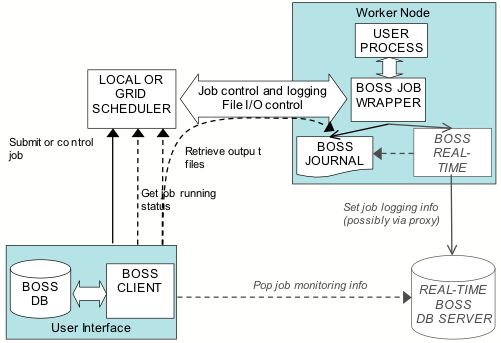
\includegraphics[width=0.85\linewidth]{boss/boss_information_flow}
  \caption{New BOSS information flow.~\cite{citeulike:880984}
  \label{fig:boss_information_flow}}
\end{figure}

Monitoring was optional and the information returned via a monitoring database server. These databases could be installed by the individual user or, more likely, by a Tier-1/2 for all its users. Information was sent from jobs to the dedicated monitoring server via a specialist monitoring framework. Multiple frameworks were available including a custom protocol~\cite{citeulike:880984} and MonaLisa~\cite{citeulike:880975}. Information would then reside in this database until retrieved by the user with the BOSS client. The monitoring information had a limited lifetime and could not be used to populate the logging database.

Figure~\ref{fig:boss_information_flow} shows the new BOSS components and information flow. The constituent jobs in the task were submitted via a batch scheduler to a worker node. Once the job started BOSS activated the monitoring and chainer. The chainer took responsibility for the users workflow, as illustrated in Figure~\ref{fig:boss_chain}. Logging and monitoring information were written to the journal file and, if requested by the user, sent to the monitoring database. The user BOSS client tools retrieved information from the monitoring database and hence allowed users to track their jobs. Once the job finished the user retrieved the output and BOSS updated the logging database from the journal file.

%show picture - BOSS architecture pic
\begin{figure}[!tp]
  \centering
  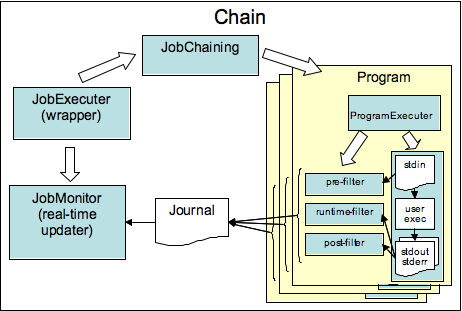
\includegraphics[width=0.85\linewidth]{boss/boss_chain}
  \caption{BOSS runtime components.~\cite{citeulike:880984}
  \label{fig:boss_chain}}
\end{figure}

\section{Task Definitions}
To create a task the user required a syntax that could express the hierarchy. A logical choice for this was XML, which naturally provides for nested hierarchies of tasks, jobs and applications. Figure~\ref{fig:boss_xml} shows an example task specification. This shows a task composed of 100 chains each composed of one program. The ``iterator'' concept was introduced to simplify writing specifications. This provided a looping mechanism within the specification. The iterator was replaced by the required number of chains (or other inner element) and the iterator name was replaced by its value as of that loop iteration. 

%\begin{figure}[!tp]
%  \centering
%  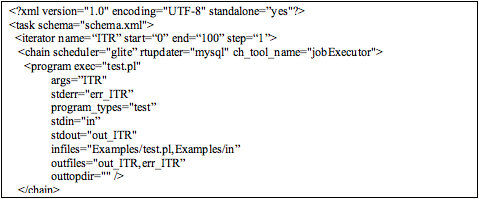
\includegraphics[width=0.85\linewidth]{boss/boss_xml}
%  \caption{An example XML task specification showing a task composed of 100 chains of one program.~\cite{citeulike:880984}
%  \label{fig:boss_xml}}
%\end{figure}
\begin{figure}[!tp]
\begin{verbatim}
<?xml version="1.0" encoding="UTF-8" standalone="yes"?>
	<task schema="schema.xml">
	  <iterator name="ITR" start="0" end="100" step="1">
	   <chain scheduler="glite" rtupdater="mysql" ch_tool_name="jobExecutor">
	     <program exec="test.pl" 
	              args="ITR" 
	              stderr="err_ITR"
	              program_types="test"
	              stdin="in"
	              stdout="out_ITR"  
	              infiles="Examples/test.pl,Examples/in"
	              outfiles="out_ITR,err_ITR"
	              outtopdir="" /> 
	   </chain>
	  </iterator>
	</task>
\end{verbatim}
\caption{An example XML task specification showing a task composed of 100 chains of one program.~\cite{citeulike:880984}\label{fig:boss_xml}}
\end{figure}
There were two standard XML parsing mechanisms: Document Object Model (DOM) and Simple Api for Xml (SAX). DOM provided a navigable object tree representing the document. SAX provided an event-driven system for calling a given function when a certain tag was encountered. For instance when a task definition was encountered, a function would be called to instantiate a task object. There were advantages and disadvantages to both methods: SAX was generally faster but required development of functions to create tasks and jobs (which would need updating with any schema changes) whereas DOM provided the entire document as an accessible object but had greater memory requirements. 

It was decided that the greater speed of SAX was unnecessary for this project as users would generally only create tasks with O(1000) jobs and communication with external services, PubDB and LCG, would dominate any latencies. Due to the predicted size of users tasks the possible higher memory use of DOM was not considered a problem. Thus it was decided to use DOM with the document object as the internal task data structure. This was an idea taken from web browsers where internally an HTML page is stored as a DOM object. In the future when more users create larger tasks these performance issues may become important however it was viewed that in the short-medium term these performance issues were not be important.

%Once the choice of parsing method had been made the choice of parser implementation remained. Several mature parser libraries which could handle both DOM and SAX existed. Requirements included ease of install and wide availability amongst LCG sites (It was required at runtime to allow the chain to read its workflow). In order to allow the DOM object to be used for the task representation it was desirable for BOSS to be able to obtain pointers directly at a tasks children i.e. the chains and their children i.e. the executables. This would allow the passing of a start and end pointer to functions that operated on a subset of the chains. This violated the object orientedness of the system and only a few libraries could be used in this way.

%CMS and LCG had decided on Xerces produced by the Apache foundation. This was a mature and very capable library however it involved a reasonable install (11MB), was fairly complicated and did not provide the facility that would allow BOSS to get direct access to a documents children. For these reasons another parser was chosen, libxml2. This has been developed by the Gnome project and is a C library that provided mechanisms for directly accessing the children of a documnet.

%Wrapping the XML libraries was a BOSS class called XMLDoc. This class provided all neccesary functions for BOSS including parsing, attribute/child modification and the ability to obtain pointers (of the same type) to children that statsfied a query.

The iterator concept required either support from the task object or modification of the XML before parsing because XML does not support the concept of iterators. The latter could be achieved by use of Extensible Stylesheet Language Transformations (XSLT). This is a language capable of describing transformations of an XML document and is usually used to convert XML to viewable HTML. XSL transforms were designed to execute certain actions when a particular XML structure was encountered, but XSL lacks support for loop structures and did not fully support variable modification. The combination of these resulted in a limit of one iterator tag. If more than one tag was included in a document the two would interfere and only the values of one would be correctly replaced. This was not regarded as a major limitation because the most common usage was a single iterator of chains within a task.

%The GNOME project also provided an XSLT library called libxslt.

%XSL transforms were designed for parsing XML and outputting certain strings when a particular piece of XML is reached not for implementing loop structures. A way round this was found but resulted in the limitation of a maximum of one iterator tag, this was because it couldn't correctly replace the text in both iterations only the last iterators text was replaced. This wasnt a problem as most use involved a single iterator cycling over the chains in a task.

\section{API}
The previous BOSS API provided the same commands as the command line client with no fine-grained control or feedback. It was decided that a more complete API that allowed greater control and functionality was required.

% BOSS was written in C++ so a C++ API could be used by the BOSS CLI and external clients.

The API needed to provide functionality suitable for CMS analysis, production and individual users. The API was split into two: user commands (e.g. submit, query) and administration tasks (e.g. register scheduler, job types). The administrator commands could only be run by someone with database administrator privileges. 

%The Administrator commands included registration of job types, batch schedulers and chainer tools. 

%The user API provided the facility for task declaration, submission, querying and output retrieval.

As with the rest of BOSS these API's were written in C++. However, both the CMS production and analysis frameworks were written in Python. It is possible for a Python program to call a C++ API but this required significant effort on the part of the client developer. As a number of CMS applications, both current and proposed, were written in Python it was decided to provide a Python version of the API's. It was felt that the best way to do this was to wrap the C++ API hence ensuring that the two were continually synchronised. 

The wrapping code had to provide a number of features, including:
\begin{itemize}
\item Input argument validation;
\item Conversion of input Python arguments to C++ datatypes;
\item Invocation of the corresponding C++ method; and
\item Conversion of output values to Python datatypes.
\end{itemize}

Advanced C++ features such as polymorphism and exception handling required more complex wrapping code. This problem had been encountered before in computer science and a number of tools had been developed to automate the process. These included SWIG~\cite{citeulike:881608}, SIP~\cite{citeulike:881611} and BOOST.Python~\cite{citeulike:881616}. These tools could generate Python code from the C++ sources and their use was less error prone and faster than writing the code manually.

Each tool implemented a slightly different wrapping strategy. SWIG generated wrapper code from the C++ header files that was then built against the C++ libraries. It had support for multiple scripting languages including Python, Perl, Ruby and many others, and was widely adopted with good documentation. 

SIP was originally designed to generate Python bindings for a graphical user interface. It used a similar method to SWIG with separate wrapper code generation and build steps. It had the disadvantages that it was specifically designed for one application and not as a general-purpose tool. It also only worked with Python and had minimal documentation. 

BOOST.Python took a different approach, called template metaprogramming, where each function was declared in Python with a special syntax. By calling this function BOOST automatically called the appropriate C++ code. This required a modern compiler to work correctly and only supported the Python language.

%The wrapping added a significant overhead to any function call however this was likely to be small compared to the overheads associated with communication with the database and batch scheduler. ref study on speed.

Due to the documentation and the support for multiple languages it was decided to use SWIG to create the API bindings. The wrapping added a significant overhead to any function call and SWIG was considerably slower than the other tools~\cite{citeulike:881635}. However this overhead was expected to be small compared to the overheads associated with database or scheduler communication as a typical session involved O(10) Python method calls.

%however this was likely to be small compared to the overheads associated with communication with the database and batch scheduler. SWIG was considerably slower than other methods however as a typical session involved O(10) Python method calls the effect was acceptable~\cite{citeulike:881635}.

%%%%%
% Do we need the details?
%SWIG required directing by a file listing the Python module to build and the functions to wrap. This was simplified as you could simply tell SWIG to include the contenets of the C++ header file.
%%%%%

Only the generation of the Python bindings required SWIG, while the building and linking did not. The generation step was performed by a developer during the building of a release. With the generated code added to the release the user only needed to build everything together. Thus there was no requirement for SWIG to be available on the user's machine. 
%Binary distribution was also available.


% emphasize diff between distributing source code and binaries

%%%%%
%Problems with previous versions
%Problems encountered by GROSS
%improvements from GROSS
%Others - i.e. chainning
%
%New Architecture
%
%XML task specification
%DOM
%Original idea to have XML DOM represent task i.e. like web page - ref and show feasible
%libxml2 - easy and common
%requirement for ability to go down hiearchy modifying (what about rest - why?)
%transform - iterator - not ideal - limitation
%
%Pyhton API for CRAB + ProdAgent
%%%%%

\section{Conclusion}
Use by both the CMS production and analysis systems required a number of enhancements to BOSS. These included the task concept and better logging mechanisms. An improved API was introduced with greater functionality and multi-language support. To support the task structure a new XML-based task specification was developed. 


% theory chapter
\chapter{Higgs mechanism and Supersymmetry}

\section{Introduction}
The Standard Model (SM) of particle physics has proved to be one of the most successful theories in physics. There are many good overviews of the SM, including~\cite{HALZEN} and~\cite{GRIFFITHS}. This chapter focuses on one of the less satisfactory elements of the Standard Model the origin of particle mass, for reasons that will be discussed later. It describes a proposed solution, concentrating on elements that are pertinent to the experimental study presented at the end of this thesis.

The Standard Model describes spin-1/2 matter particles, known as fermions, and their interactions mediated via the exchange of spin-1 particles, known as bosons (with the exception of gravity, which is mediated via a spin-2 boson). The bosons include the photon ($\gamma$), which mediates the electromagnetic force, the $\mathrm{W^{\pm}}$ and Z, responsible for the weak force, gluons, responsible for the strong force, and gravitons that mediate gravity.

In the Standard Model particle wavefunctions are invariant under local phase (gauge) transformations, a principle known as local gauge symmetry. The requirement for fermions to be invariant under the U(1) local gauge transformation results in the coupling of fermions and massless photons, i.e. electromagnetism. Similarly SU(2) and SU(3) invariance forms the basis of the weak and strong forces.

The Standard Model unifies the electromagnetic and weak forces with the electroweak theory of Glashow, Weinberg and Salam~\cite{Salam:1964ry}. This theory states that both forces are representations of the same fundamental process. Two new charges are introduced, weak isospin (T) and hypercharge (Y), which together with four new fields, $\mathrm{W^{1,2,3}_{\mu}}$ and B are invariant under SU$(2)_\mathrm{L}$ $\times$ U$(1)_{\mathrm{Y}}$, where L signifies that only left-handed particles take part in the weak interaction. These fields mix to form the $\gamma$ (represented by the field A), $\mathrm{W^{\pm}}$ and Z:

\begin{equation}
	A_{\mu} = B_{\mu} \cos{\theta_{W}} + W_{\mu}^{3} \sin{\theta_{W}}
	\label{eqn:A}
\end{equation}
\begin{equation}
	W_{\mu}^{\pm} = \frac{1}{\sqrt{2}}(W_{\mu}^{1} \mp W_{\mu}^{2})
	\label{eqn:W}
\end{equation}
\begin{equation}
	Z_{\mu} = - B_{\mu} \sin{\theta_{W}} + W_{\mu}^{3} \cos{\theta_{W}}
	\label{eqn:Z}
\end{equation}

%\begin{equation}
%	W_{\mu}^{3} = A^{\mu}\sin{\theta_{W}} + Z^{\mu}\cos{\theta_{W}}
%	\label{eqn:Z}
%\end{equation}

where $\theta_{W}$ is the Weinberg angle. 

The local gauge invariance that introduced the massless photon has a similar effect on all the bosons and thus requires them all to be massless. However experiment has shown that both the $\mathrm{W^{\pm}}$ and Z are massive. The introduction of explicit mass terms for these fields destroys gauge invariance, which is the foundation of the SM. The Higgs mechanism~\cite{citeulike:918519} represents a possible solution to this problem.

%A source for particle masses is presented along with a further problem that this introduces. A solution to this problem is given by a theory known as Supersymmetry (SUSY). This chapter describes SUSY and elements of the theory that impact on the experimental search presented later.   

%one problem with...

\section{Higgs mechanism}
%The standard model (SM) of particle physics has proved extremely successful at describing the electro-weak and strong interactions. One of its major limitations is the need to explain the massive vector bosons, $\mathrm{W^{\pm}}$ and Z. Introducing explicit mass terms destroys the Lagrangians gauge invariance, making the theory un-renormalisable. The Higgs mechanism is a means for giving the $\mathrm{W^{\pm}}$ and Z mass while retaining gauge invariance. 

Boson masses may be introduced through a process known as spontaneous symmetry breaking, which occurs when the Lagrangian is invariant under local gauge transformations but the ground (vacuum) state is not. The electroweak $\mathrm{SU(2) \times U(1)_{Y}}$ symmetry must be broken to give mass to the $\mathrm{W^{\pm}}$ and Z whilst leaving the $\gamma$ massless. This can be accomplished with the addition of a complex scalar doublet, $\phi$:

\begin{equation}
	\phi = \binom{\phi^{+}}{\phi^{0}}
\end{equation}

%pic from Filip

%\begin{equation}
%	\phi = \phi_{1} + i \phi_{2}
%\end{equation}

%\begin{equation}
%	\phi^{*}\phi = \phi_{1}^{2} + \phi_{2}^{2}
%\end{equation}

The standard model Lagrangian gains additional terms:

\begin{equation}
	\mathcal{L} = D_{\mu}\phi^{*}D_{\mu}\phi - V(\phi) = D_{\mu}\phi^{*}D_{\mu}\phi + \mu^{2}\phi^2 - \lambda \phi^{4}
	\label{eqn:lagrangian}
\end{equation}
%1.21 filip

with the covariant derivative

\begin{equation}
	D_{\mu} \phi = (\partial_{\mu} + igW_{\mu}^{a}T^{a} + ig^{\prime}B_{\mu})\phi
\end{equation}

where $T^{a}$ is the $\mathrm{SU(2)}$ group generator and g(g$^{\prime}$) is the $W_{\mu}^a$ ($B_{\mu}$) coupling constant. $\mu$ and $\lambda$ are the $\phi$ mass parameter and self-interaction, respectively. The first term of Equation~\ref{eqn:lagrangian} describes the kinetic part of the Lagrangian and the last two terms the potential, V($\phi$).

%\begin{equation}
%	van der aa 1.3
%\end{equation}


%. Requiring the vacuum to be invariant under implies that $\phi$ is constant in the vacuum state. 

Two possible potential forms exist depending on the value of $\mu^2$, as shown in Figure~\ref{fig:Higgs_potential}. In the case of $\mu^{2} > 0$ the potential has a minima at $\phi = 0$. If $\mu^{2} < 0$ the minima form a circle where

\begin{figure}[bt]
  \centering
  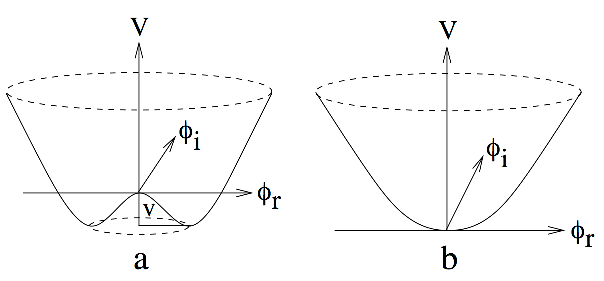
\includegraphics[width=0.55\textwidth]{theory/Higgs_potential}
  \caption{The Higgs potential as a function of a complex scalar field with negative (a) and positive (b) mass parameter. $\phi_{r}$ ($\phi_{i}$) represents the real (imaginary) component of $\phi$.
  \label{fig:Higgs_potential}}
\end{figure}

\begin{equation}
	\phi^2 = \frac{\mu^{2}}{2 \lambda} = \frac{v^2}{2} \qquad \mathrm{where\,} v = \frac{\mu}{\sqrt{\lambda}}
	\label{eqn:minima}
\end{equation}

%Once we have discovered the possible values for the minima we can expand about an arbitrary point on the circle. As the Lagrangian is invariant under rotations in the complex plane any value of $\theta$ may be taken, for convenience we choose $\theta$ = 0:
%.see van der AA 1.3

%The vacuum expectation value of $\phi$ is thus degenerate. The Goldstone theorem states that for 

We can then choose a vacuum expectation value (vev) for this field. The vev should be zero for the charged component of the $\phi$ field to preserve the electromagnetic, $\mathrm{U(1)_{EM}}$, symmetry. Expanding $\phi$ arbitrarily about its vev results in one massive and three massless bosons. The massless bosons are a result of the Goldstone theorem, which states that for each broken symmetry, a massless field will result. These particles are known as Goldstone bosons and the massive boson is known as the Higgs boson.

As the expansion is arbitrary we can choose the gauge such that the Goldstone bosons are eliminated. We can expand $\phi$ as:

%\begin{equation}
%	\phi = \frac{1}{\sqrt{2}}(\frac{\mu}{\sqrt{1}} + H + i\eta)
%	\label{eqn:expansion}
%\end{equation}

%The fields H and $\eta$ are fields with zero vacuum expectation value. Inserting~\ref{eqn:expansion} into~\ref{eqn:lagrangian} we can see that the field H gains a mass term

%\begin{equation}
%	m_{H} = v \sqrt{2 \lambda}
%\end{equation}

%While $\eta$ is a massless particle called a Goldstone boson. This massless particle is a direct consequence of the degenerate nature of the vacuum. 

%Egede thesis
%The Higgs mechanism has been developed to remove the Goldstone boson. To begin with the derivatives are replaced by their covariant forms. 

%One ground state is:

%\begin{equation}
%	\langle \phi \rangle = \frac{1}{\sqrt{2}} \binom{0}{v}
%\end{equation}

%where:

%\begin{equation}
%	v = \frac{\mu}{\sqrt{\lambda}}
%\end{equation}
	
%Instead of making an arbitrary choice of the minima we may choose it such that Goldstone boson is eliminated. 

\begin{equation}
	\phi(x) = e^{iT^{a}\theta_{a}(x)} \frac{1}{\sqrt{2}}\binom{0}{v + H(x)}
	\label{eqn:unitarygauge}
\end{equation}

Taking Equations~\ref{eqn:unitarygauge} and~\ref{eqn:lagrangian} together with the physical electroweak fields~\ref{eqn:A},~\ref{eqn:W} and~\ref{eqn:Z}, we obtain the masses:

%\begin{equation}
%	M_{W} = \frac{v g_{2}}{2} \\qquad M_{Z} = \frac{v}{2}\sqrt{g_{2}^{2} + g_{1}^{2}} \\qquad M_{A} = 0
%\end{equation}

\begin{equation}
	m_{W} = m_{Z} \cos{\theta_{W}} = \frac{gv}{2}, \qquad m_{A} = 0
\end{equation}

%As a consequence of this the gauge bosons acquire a mass. 

Thus the Higgs mechanism, by utilising spontaneous symmetry breaking and a convenient choice of gauge, gives mass to the $\mathrm{W^{\pm}}$ and Z while keeping the $\gamma$ massless.   

The Standard Model also requires a mechanism for explaining the fermion masses. These can be introduced by forming interaction terms between left-handed fermions, right-handed fermions and the Higgs field. These interactions are known as Yukawa couplings. However, for each interaction a new coupling constant is required, the values of which are not predicted.

More of a problem with the Higgs mechanism is that of the Higgs mass itself. The physical mass ($m_{H}$) is related to the the bare mass ($m_{H_{0}}$) with corrections from loop diagrams ($\Delta m_{H}$), as illustrated in Figure~\ref{fig:Higgs_correction}.

\begin{equation}
	m_{H}^2 = m_{H_{0}}^{2} + \Delta m_{H}^2
\end{equation}

The fermion contribution to the correction is:

\begin{equation}
	\Delta m_{H}^{2} \approx O(-\Lambda^{2})
\end{equation}

where $\Lambda$ represents the scale where new physics is introduced and the theory no longer holds. If no new physics occurs at high energy scales then the cut-off becomes the Planck scale, $10^{19}$\GeVcc. An upper limit on the Higgs mass can be determined from the WW scattering crosssection which at high energies becomes greater than unitarity for $m_{H} > 1\TeVcc$~\cite{citeulike:918524}. To cancel the correction and result in the Higgs boson mass of $\sim1\TeV$ the bare mass must be $\approx 10^{19} \GeVcc$. While mathematically possible this is aesthetically displeasing and is known as the fine tuning problem.

\begin{figure}[bt]
  \centering
  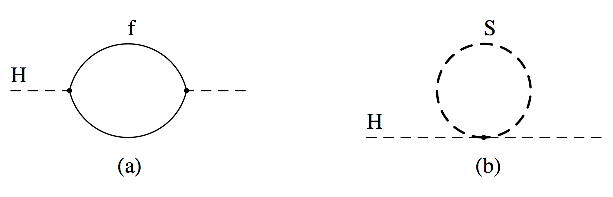
\includegraphics[width=0.5\textwidth]{theory/Higgs_correction}
  \caption{Corrections to the Higgs mass from fermion (a) and boson (b) loops.~\cite{citeulike:681336}
  \label{fig:Higgs_correction}}
\end{figure}

As well as corrections from fermions, boson loops also contribute. Their contribution takes the same form as the fermion loops but with the opposite sign. Thus if a theory could be formed that matches fermions and bosons the correction would be:

\begin{equation}
	\Delta m_{H}^{2} \approx O(m_{B}^2 - m_{f}^2)
\end{equation}

which is less than $m_{H}^2$ if the fermion and boson partners have similar masses:

\begin{equation}
	m_{B}^2 - m_{F}^2 < 1 \TeVcc
\end{equation}

This indicates new physics below 1\TeV that may take the form of the theory described above. One such theory is supersymmetry.

\section{Supersymmetry}
Supersymmetry (SUSY) is a theory that relates fermions to bosons. An operator (Q) is proposed that transforms the two types:

\begin{equation}
	Q|boson\rangle = |fermion\rangle \qquad Q|fermion\rangle = |boson'\rangle
\end{equation}

As derived in~\cite{citeulike:681336} the Q operator obeys the following anti-commutation rule

\begin{equation}
	\{ Q_{\alpha}, Q_{\beta}^{\dagger} \} = 2\sigma^{\mu}_{\alpha \beta}P^{\mu}
\end{equation}

where $P^{\mu}$ is the generator of the space-time translation and $\sigma$ the Pauli matrices. Supersymmetric states are grouped together into supermultiplets, which contain a fermion and boson. These are related by the Q operator, with the particles known as each other's superpartner. It can be shown that the mass operator $P^{2}$ commutes with Q and thus that the superpartners have equal mass~\cite{citeulike:681336}. Also the Q operator commutes with the gauge symmetries therefore the superpartners must have equal charge, weak isospin, hypercharge and colour. 

It is clear that no superpartners of any known particles have been discovered with the same mass and quantum numbers except spin, hence supersymmetry must be broken. This is possible because the superpartners of the Standard Model particles may have an explicit mass term in their Lagrangian without violating electroweak symmetry~\cite{citeulike:681336}. The Supersymmetry breaking mechanism is not understood and most phenomenological models parameterize it.

\section{The Minimal Supersymetric Standard Model \label{sec:mssm}}
The Minimal Supersymmetric Standard Model (MSSM) is the simplest supersymmetric extension to the standard model that aims to minimise the numbers of superfields and interactions. For each SM particle a new superpartner is required.

Two Higgs doublets with different hypercharge are required to give mass to the up and down type fermions: 

\begin{equation}
	\phi_{u} = (\phi_{u}^{+}, \phi_{u}^{0}) \qquad \phi_{d} = (\phi_{d}^{0}, \phi_{d}^{-}) 
\end{equation}

The vev of these fields may be written:

\begin{equation}
	\langle \phi_{u}\rangle = \binom{0}{v_u} \qquad \langle \phi_{d}\rangle = \binom{v_d}{0}
\end{equation}

These can be related to the $\mathrm{W^{\pm}}$ mass via:

\begin{equation}
	v_{u}^{2} + v_{d}^{2} = \frac{2m_{W}^{2}}{g} \approx (174 \GeVcc)^{2}
\end{equation}

The ratio of the two vev's is not predicted, and we define this ratio as:

\begin{equation}
	\tan\beta = \frac{v_u}{v_d}
\end{equation}

After $\mathrm{SU(2) \times U(1)_{Y}}$ symmetry breaking three of the Higgs degrees of freedom are taken by the $\mathrm{W^{\pm}}$ and Z, leaving five massive Higgs bosons: a charge parity (CP) symmetry odd neutral scalar $A$, two CP even neutral scalars $h$ and $H$ and a pair of charged scalars $H^{+}, H^{-}$:

\begin{equation}
	A = \sqrt{2}(\cos{\beta}\ \mathrm{Im}[\phi^{0}_{u}] + \sin{\beta}\ \mathrm{Im}[\phi^{0}_{d}])
\end{equation}
\begin{equation}
	H^{\pm} = (\cos{\beta}\ \phi^{\pm}_{u} + \sin{\beta}\ \phi^{\mp*}_{d})
\end{equation}
\begin{equation}
	\left(
	\begin{array}{c}
		h \\
		H \\
		\end{array} \right) = \sqrt{2} \left(
	\begin{array}{cc} 
		\cos{\alpha} & -\sin{\alpha} \\ 
		\sin{\alpha} & \cos{\alpha} \\ 
	\end{array} 
	\right)
	\left( \begin{array}{c} 
		\mathrm{Re} [H_{u}^{0}] - v_u\\ 
		\mathrm{Re} [H_{d}^{0}] - v_d \\
	\end{array}
	\right)
\end{equation}

The mixing angles $\alpha$ and $\beta$ are determined at tree level by:

\begin{equation}
	\cos^2{(\beta - \alpha)} = \frac{m_h^2(m_Z^2 - m_h^2)}{m_A^2(m_H^2 - m_h^2)}
	\label{eqn:alpha}
\end{equation}

%\subsection{Theoretical constraints}
Theoretical constraints can be applied to $\beta$ as the fermions masses are determined by Yukawa couplings. The requirement that fermion masses do not diverge leads to the constraint $1.2 \lesssim \tan{\beta} \lesssim 60$.~\cite{kane:2002}

At tree level the Higgs masses depend only on two parameters, $m_{A}$ and $\tan{\beta}$:
\begin{equation}
	m_{H^{\pm}}^2 = m_{A}^2 + m_{W}^2
\end{equation}
\begin{equation}
	m_{h,H}^2 = \frac{1}{2}\left( m_{A}^2 + m_{Z}^2 \mp 
	\sqrt{(m_{A} + m_{Z})^2 - 4m_{Z}^2 m_{A}^2 \cos{2\beta})}
	\right)
	\label{eqn:m_h}
\end{equation}

From~\ref{eqn:m_h} one can obtain an upper bound on $m_{h}$:

\begin{equation}
	m_{h} \le m_{Z}|\cos{2\beta}|
\end{equation}

However loop corrections modify this. The maximum one loop contribution is

\begin{equation}
	m_{h}^2 \lesssim m_{Z}^2 + \frac{3g^2m_{t}^4}{8\pi^2m_{W}^2} 
	\left[ 
	  \ln \left( \frac{M_{S}^2}{m_{t}^2} \right) + \frac{X_{t}^2}{M_{S}^2} 
	    \left( 1 - \frac{X_{t}^2}{12 M_{S}^2} \right)
	\right] 
\end{equation}

where $M_{\mathrm{SUSY}} = M_{\tilde{t}} = M_{\tilde{b}}$, $M_{S}^2 = M_{\mathrm{SUSY}}^2 + m_{t}^2$ and $X_{t} = (A_{t} - \mu \cot{\beta})$.\footnote{A tilde indicates the superpartner of the indicated particle.} $\mu$ is the Higgs mixing parameter and $A_t$ the trilinear Higgs-$\tilde{s}$ coupling. This correction increases with $X_t$ reaching its maximal value, \mhmax, at $X_t = \sqrt{6}M_S$:

\begin{equation}
	\mhmax \lesssim 130 \GeVcc
\end{equation}

This number is calculated with a top mass of 175\GeVcc and assuming that no superpartner masses ($M_{\mathrm{SUSY}}$) exceed 1\TeVcc. 

Two Higgs mass regimes may be identified depending on the ratio of $m_{A}$ and \mhmax:

\begin{itemize}
	\item $m_{A} \gg \mhmax$: $m_A \sim m_H \sim m_{H^{\pm}}$ with h behaving like the SM Higgs.
	\item $m_{A} \ll \mhmax$: $m_A \sim m_h$ with H behaving like the SM Higgs.
\end{itemize}

The couplings of the MSSM Higgs sector compared to the SM are shown in Table~\ref{tab:MSSMcoupling}. It can be seen that the h and H bosonic couplings are greatly suppressed compared to the SM couplings. In the two mass regimes the couplings simplify. For large $m_{A}$ one can derive from Equation~\ref{eqn:alpha} that $\cos(\beta - \alpha) \ll 1$. This implies that $h$ coupling to bosons will be similar to the SM Higgs boson and the boson couplings of the $H$ will be strongly suppressed, while the coupling of both the $A$ and $H$ will be enhanced by a factor $\tan{\beta}$ for down-type fermions. This may prove useful in experimental searches where down-type final state particles are sought. This is especially true in the case of  b quarks and $\tau$ leptons since the Higgs coupling is proportional to mass.

\begin{table}[tbp]
	\centering
	\begin{tabular}{|l|c|c|c|}
	\hline
	coupling & $h$ & $H$ & $A$ \\ \hline
	up-type fermions & $\cos{\alpha} / \sin{\alpha}$ & $\sin{\alpha} / \sin{\beta}$ & $\cot{\beta}$ \\ \hline
	down-type fermion & $- \sin{\alpha} / \cos{\beta}$ & $\cos{\alpha} / \cos{\beta}$ & $\tan{\beta}$ \\ \hline
	W,Z & $\sin{(\beta - \alpha)}$ & $\cos{(\beta - \alpha)}$ & 0 \\ \hline
	\end{tabular}
\caption{MSSM couplings for the neutral Higgs bosons.\label{tab:MSSMcoupling}}
\end{table}

\section{Summary}
The Higgs mechanism provides a means for giving mass to the $\mathrm{W^{\pm}}$ and Z bosons. Various problems have been identified with the Higgs mechanism that supersymmetric theories aim to solve. The MSSM is the simplest supersymetric extension to the Standard Model and the phenomenology of its Higgs sector has been explained. Neither Higgs bosons nor any supersymmetric particles have so far been discovered. They are the prime targets of the next generation of particle experiments and if they exist with masses $< 1\TeVcc$ they should be seen at LHC.

%Tau calibration chapter
\chapter{$\tau$ tagging and calibration}

\section{Introduction}

%%%%%
% Need for a dedicated tau calibration
% ECAL/HCAL not perfect
% MET
% Calorimeter response
% collimated jet
% lots of ECAL
% Narrow jet - 0.4 cone instead of 0.5
% other properties i.e. lifetime - but i dont use it, so out in or not?
% tau decays - i.e. 1,3,5 prong
%%%%%

The $\tau$ lepton will be a useful signature of many physics processes at CMS. The $\tau$ decays via the weak mechanism with a characteristic decay time of $\tau$ = $290\times 10^{-15}$s ($c\tau$ = 87.11\micron)~\cite{pdg2006}. The $\tau$ primarily decays hadronically with a branching ratio of 65\%, forming a $\tau$ jet. When the jet has large transverse momentum, $\PT \gg M_{\tau}$ (1.78~\GeVcc), the constituent hadrons' momentum transverse to the jet axis is small resulting in a highly collimated, narrow jet. 77\% of hadronic decays consist of a single charged hadron and a number of neutral pions (one prong decays). The majority of the remainder of the hadronic decays involve 3 charged particles(three prong decays). Decays with 5 charged particles also occur but are much rarer.

The standard CMS reconstruction cone size ($\mathrm R = 0.5$) was too large for $\tau$ jets, introducing detector noise. Consequently this was optimised during this study. Figure~\ref{fig:tau_scale_cone_size} shows the energy containment and resolution, $\sigma(E)/<E>$, for $\tau$ jets as a function of reconstruction cone size for various \ETMC ranges. These plots show that a cone size of 0.4 was appropriate for $\tau$ jets, with a 98\% energy containment and good resolution.

\begin{figure}[tb]
  \centering
  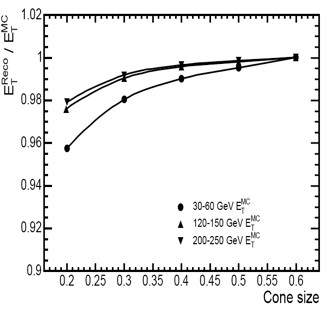
\includegraphics[width=0.49\textwidth]{tau/tautag_cont_vs_cone}
  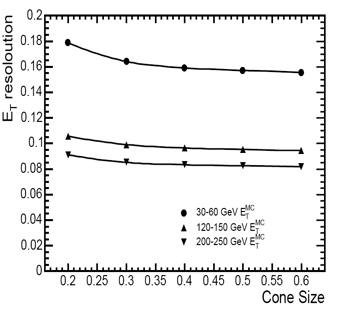
\includegraphics[width=0.49\textwidth]{tau/tautag_res_vs_cone}
  \caption{The $\tau$ jet energy scale, normalised to that obtained with a 0.6 cone, (left plot) and resolution, $\sigma/<E>$, (right plot) as a function of reconstruction cone size.~\cite{CMS_TDR_PHYS_vol1, citeulike:800614}
  \label{fig:tau_scale_cone_size}}
\end{figure}

\section{$\tau$ tagging}

%%%%%
% Tracker isolation - same Z vertex - IP cut to remove fake tracks
% ECAL isolation
% HLT CaloPxl
% impact paramater and tau mass and flight-path
%%%%%

A number of $\tau$ tagging methods have been developed for CMS \cite{CMS_TDR_PHYS_vol1, citeulike:800614}. Some of the most common techniques are presented below.

\subsection{Tracker isolation~\label{sec:tracker_isolation}}
\begin{figure}[!hHtb]
  \centering
  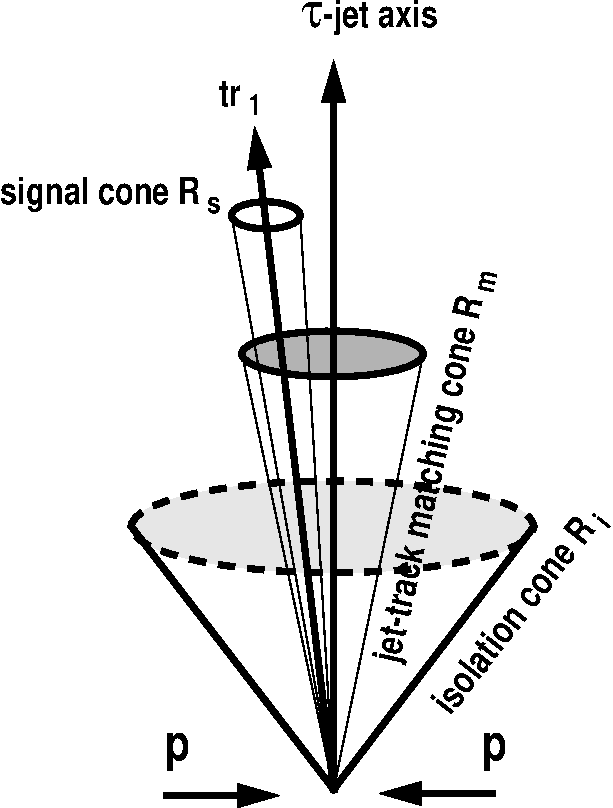
\includegraphics[width=0.45\textwidth]{tau/tautag_sketch_tauisol}
  \caption{$\tau$ identification method using the tracker.~\cite{CMS_TDR_PHYS_vol1, citeulike:800614}
  \label{fig:tracker_isol_sketch}}
\end{figure}

The tracker isolation method sought a narrow isolated $\tau$ jet. The principle is shown in Figure~\ref{fig:tracker_isol_sketch}. Tracks with \PT greater than a defined value, $\mathrm{p_{T}^{m}}$, with respect to the beam were sought within a matching cone of radius $\mathrm{R_{m}}$ about the calorimeter jet axis. The highest \PT track with unsigned transverse impact parameter $\mathrm{IP_{T} < 300}$\micron was defined to be the leading track ($\mathrm{tr_{1}}$). The $\mathrm{IP_{T}}$ cut removed fake tracks reconstructed from hits left by soft particles in QCD jets~\ref{fig:tau_ip}. Tracks within the cone $\mathrm{R_{S}}$ centred on $\mathrm{tr_{1}}$  with a z-impact parameter $\mathrm{z_{tr}}$ close to the z-impact parameter of the lead track $\mathrm{z_{tr}^{ltr}}$ ($\mathrm{|z_{tr} - z_{tr}^{ltr}| < \Delta z_{tr}}$) were assumed to come from the $\tau$ and termed ``signal tracks''. Other tracks within the cone $\mathrm{R_{i}}$ with $\mathrm{P_{T}}$ w.r.t the beam greater than $\mathrm{P_{T}^{i}}$ and satisfying $\mathrm{|z_{tr} - z_{tr}^{ltr}| < \Delta z_{tr}}$ were termed ``isolation tracks''. The isolation criteria required zero isolation tracks.

\begin{figure}[htb]
  \centering
  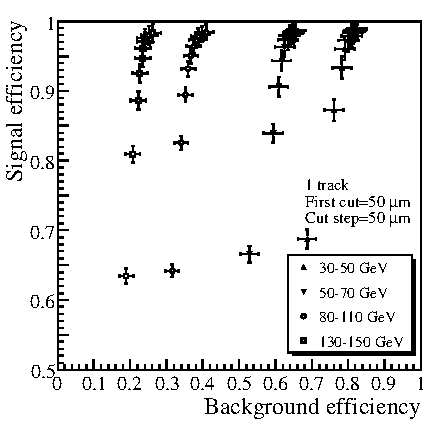
\includegraphics[width=0.49\textwidth]{tau/tautag_ip2d_1.pdf}
  \caption{$\tau$ tagging efficiencies for 1-prong $\tau$ jets and 4 \ETMC bins of 1-prong QCD multi jets. \ETMC obtained with Monte Carlo  particle jets excluding neutrinos. The upper cut on transverse impact parameter of the lead track is varied between $50-550~\micron$.~\cite{CMS_TDR_PHYS_vol1, citeulike:800614}
  \label{fig:tau_ip}}
\end{figure}

\begin{figure}[tb]
  \centering
  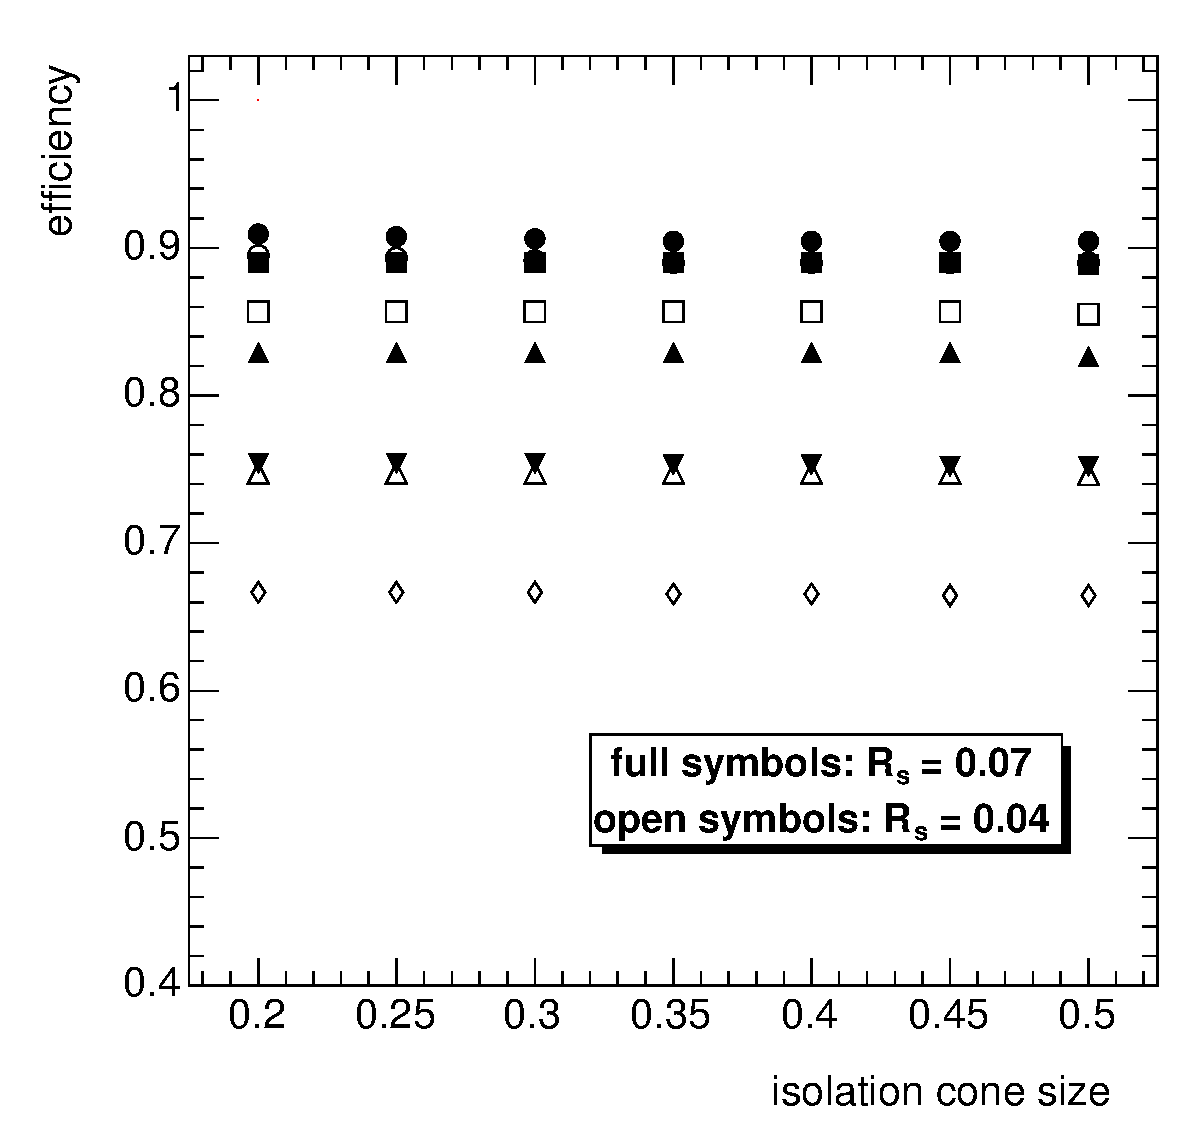
\includegraphics[width=0.45\textwidth]{tau/tautag_trkisol_tau}
  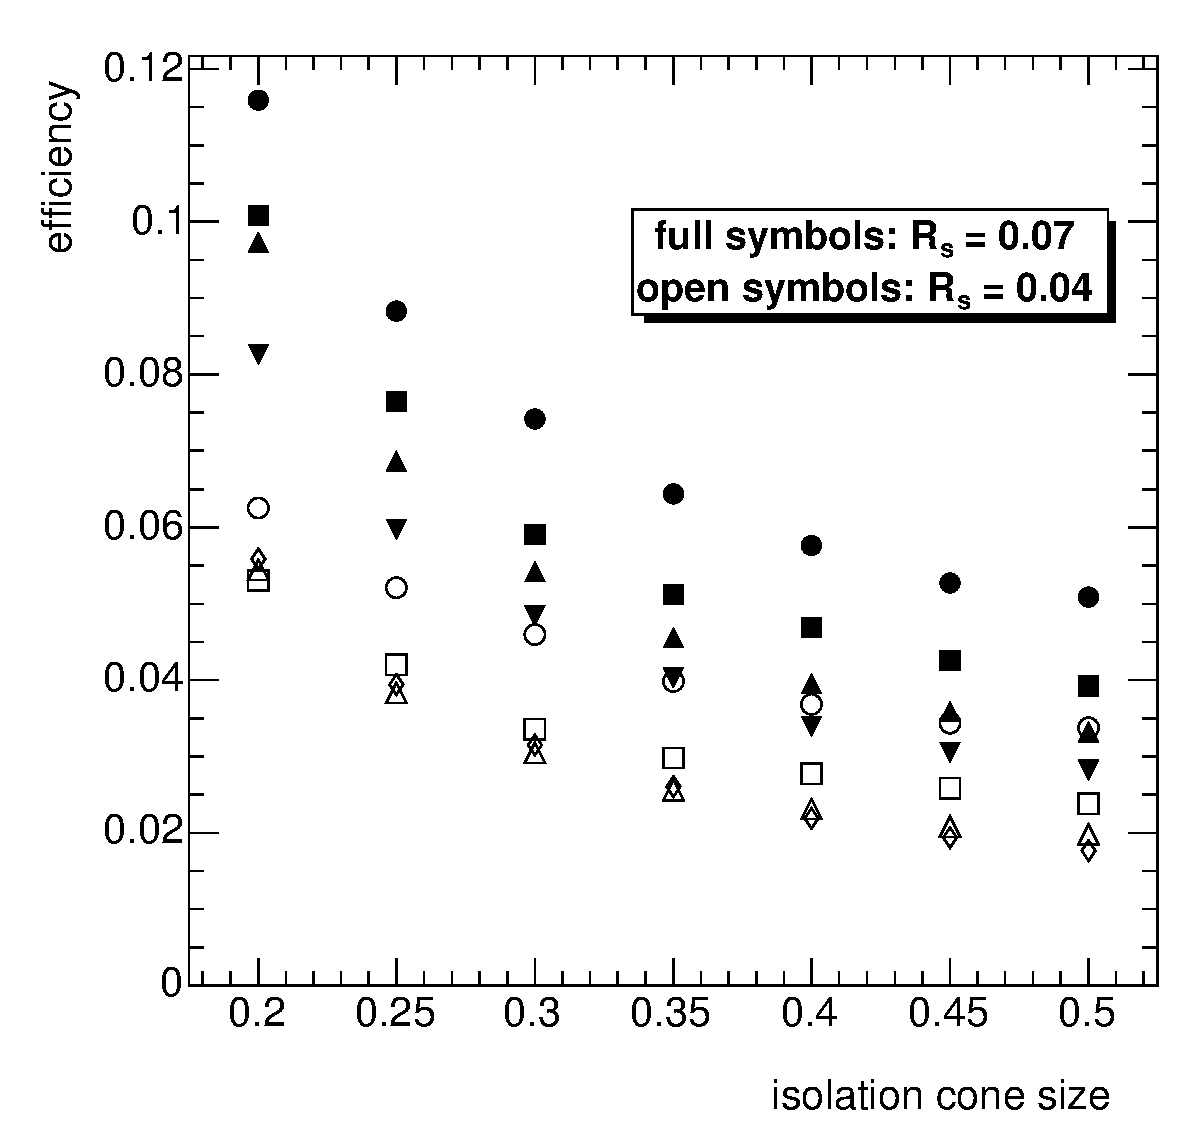
\includegraphics[width=0.45\textwidth]{tau/tautag_trkisol_qcd}
  \caption{The tracker isolation efficiency for $\tau$ jets (left plot) and
          QCD multi-jets (right plot) as a function of the isolation cone
          $\mathrm{R_{i}}$ for 2 values of the signal cone
          $\mathrm{R_{S}}$=0.07 (full symbols) and  $\mathrm{R_{S}}$=0.04
         (open symbols). In order of decreasing efficiency the symbols
          correspond to particle level jet \ETMC bins of 130--150, 80--110,
          50--70 and 30--50 GeV. The remaining tracker isolation parameters were:
          $\mathrm{R_{m}}$=0.1, $\mathrm{p_{T}^{i}}$=1\GeVc .
          $\mathrm{\Delta z_{tr}}$=2 mm and the leading track
          $\mathrm{p_{T}}>$ 6\GeVc.~\cite{CMS_TDR_PHYS_vol1, citeulike:800614}
  \label{fig:tautag_trkisol}}
\end{figure}

Figure~\ref{fig:tautag_trkisol} shows the tracker isolation efficiency for both $\tau$ and QCD jets. Jets were reconstructed using an iterative cone algorithm with a cone size of 0.4. Tracks were reconstructed with the combinatorial track finder algorithm (the standard CMS tracking algorithm~\cite{CMS_TRKTDR}) and were required to have at least 8 reconstructed hits, 2 in the pixel detector, and a $\chi^{2} < $ 10. Tracker isolation parameters used were: $\mathrm{R_{m}}$= 0.1, $\mathrm{p_{T}^{i}}$= 1\GeVc, $\mathrm{\Delta z_{tr}}$= 2 mm and the leading track $\mathrm{p_{T}}>$ 6\GeVc. It can be seen that the efficiency of genuine $\tau$ jets was independent of $\mathrm{R_{i}}$, for the studied range, whereas QCD multi-jet rejection increased with isolation cone size. 

The well-defined number of charged particles in a $\tau$ decay lead naturally to a requirement on the number of signal tracks of 1 or 3. The effect of this can be seen in Table~\ref{tab:tautag_nprongs}. From this it was concluded that the requirement on the number of signal tracks did not significantly improve QCD multi-jet rejection vs signal efficiency.

\begin{table}[tpb]
\begin{center}
\begin{tabular}{|l|c|c|c|c|}
\hline
QCD jets; \ETMC (GeV)
& 30--50 &  50--70 & 80--110 & 130--150  \\
\hline
1 track
& 63 \%  & 72 \%  & 69 \%  & 60 \%   \\
\hline
3 tracks
&  7 \%  &  9 \%  &  9 \%  & 13 \%   \\
\hline
1 or 3 tracks
& 70 \% &  81 \%  & 78 \%  & 73 \%      \\
\hline
\hline
$\tau$ jets; \ETMC (GeV)
& 30--50 &  50--70 & 80--110 & 130--150  \\
\hline
1 track
& 81 \% & 77 \%  & 71 \%  &  70 \%   \\
\hline
3 tracks
& 10 \% & 16 \%  & 16 \%  &  20 \%   \\
\hline
1 or 3 tracks
& 91 \% & 93 \%  & 87 \%  &  90 \%    \\
\hline
\end{tabular}

\caption{The efficiency of the track counting requirement for $\tau$ and
QCD jets in different bins of \ETMC.~\cite{CMS_TDR_PHYS_vol1, citeulike:800614}
\label{tab:tautag_nprongs}}
\end{center}
\end{table}

%To further suppress low \ET QCD jets a cut on the lead track \PT > 6 \GeVc could be used.

\subsection{Electromagnetic calorimeter isolation}
$\tau$ jets produce a narrow energy deposit in the electromagnetic calorimeter. The electromagnetic isolation $\mathrm{P_{isol}}$ parameter was found to provide the best hadronic jet rejection~\cite{CMS_TDR_PHYS_vol1, citeulike:800614}. Where $\mathrm{P_{isol}}$ was defined as

\begin{equation}
\mathrm{ P_{isol} = \sum_{\Delta R < 0.40}E_{T} - \sum_{\Delta R < 0.13}E_{T} }
\end{equation}

Jets with $\mathrm{P_{isol} < P_{isol}^{cut}}$ were considered $\tau$ candidates. Figure~\ref{fig:tautag_ecal_isol} shows how the efficiency for $\tau$ and QCD multi-jets jets
 varied with $\mathrm{P_{isol}^{cut}}$. Generally a value of 5 GeV was recommended for offline analysis.

\begin{figure}[tb]
  \centering
  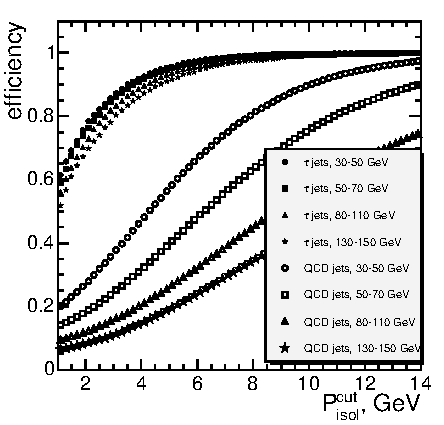
\includegraphics[width=0.55\textwidth]{tau/tautag_ecal_isol}
  \caption{Electromagnetic calorimeter isolation efficiencies for $\tau$ and QCD multi-jets as a function of $\mathrm{P_{isol}^{cut}}$.~\cite{CMS_TDR_PHYS_vol1, citeulike:800614}
  \label{fig:tautag_ecal_isol}}
\end{figure}

\subsection{Electron rejection \label{sec:e_rejection}}
An isolated electron (from a leptonic $\tau$ decay for instance) could pass both the $\tau$ jet tracker and electromagnetic isolation criteria. An offline cut on the most energetic HCAL tower in the jet was introduced to suppress these. Figure~\ref{fig:tau_e_reject} shows the hottest (maximal \ET) HCAL tower for 35 \GeV electrons and 2 \PT ranges of $\tau$s. The high electron \ET tail was due to electrons passing through $\eta-\phi$ ECAL gaps and the instrumentation gap between the barrel and endcap. Table~\ref{tab:tautag_etau_reject} shows the efficiency of this cut for $\tau$ jets and electrons. 

\begin{figure}[tb]
  \centering
  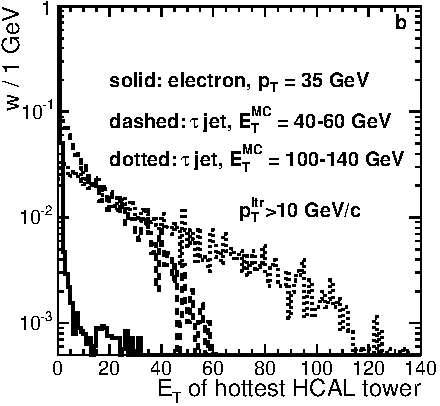
\includegraphics[width=0.45\textwidth]{tau/tautag_e_tau_reject}
  \caption{Transverse energy of maximal $E_{T}$ HCAL tower (\GeV). All histograms are normalised to unity.~\cite{CMS_TDR_PHYS_vol1, citeulike:800614}
  \label{fig:tau_e_reject}}
\end{figure}

$\mu$ lepton rejection was not investigated as energy deposited in the calorimeter was only of the order of a few \GeV, well below the jet \ET cuts used in most CMS analyses.
%%%%%%
% Move to detector chapter
%\subsection{Level-1 trigger}
%The $\tau$ trigger uses the same sliding 3 $\times 3$ window of $4 \times 4$ trigger towers as the jet trigger. Figure shows the acceptable $\tau$ energy deposit shapes. This algorithm is only applied within the region $|\eta| < 1.95$ and the jet energy is taken as the sum of the central tower.
%%%%%

\subsection{High Level Trigger\label{sec:CaloPxl}}
The High Level Trigger utilised both ECAL and tracker isolation. The HLT $\tau$ trigger was optimised for the MSSM heavy Higgs boson decaying to 2 hadronic $\tau$ jets.

\begin{table}[tb]
  \begin{tabular}{|l|c|c|c|c|c|}
   \hline
& & \multicolumn{2}{|c|}{$\tau$ jet $E_{\rm T}$ 40--60 GeV} &
    \multicolumn{2}{|c|}{$\tau$ jet $E_{\rm T}$ 100--140 GeV} \\
    \cline{3-6}
    \raisebox{1.5ex}[0cm][0cm]{cut} &
    \raisebox{1.5ex}[0cm][0cm]{electron} &
        $p_{\rm T}^{\rm ltr}>$ 10 GeV &
        $p_{\rm T}^{\rm ltr}>$ 25 GeV &
        $p_{\rm T}^{\rm ltr}>$ 10 GeV &
        $p_{\rm T}^{\rm ltr}>$ 25 GeV \\
   \hline
$>$1 GeV & 0.08 & 0.936 & 0.971 & 0.977 & 0.991 \\
   \hline
$>$2 GeV & 0.03 & 0.854 & 0.917 & 0.942 & 0.969 \\
   \hline
  \end{tabular}
  \caption{Efficiency of the transverse energy of the hottest
           HCAL tower (maximal \ET) cut for electrons \PT = 35 \GeVc and
           for different $\tau$ jet \PT ranges and lead track \PT ($\mathrm{p _{\rm T} ^{\rm ltr}}$).~\cite{CMS_TDR_PHYS_vol1, citeulike:800614}}
  \label{tab:tautag_etau_reject}
\end{table}

The recommended HLT algorithm, ``Calo+Pxl'',~\cite{CMS_TDR_PHYS_vol1, citeulike:800614} relied on ECAL isolation followed by tracker isolation using only the pixel layers. This algorithm took as seeds the 2 Level-1 $\tau$ primitives. If no second candidate was identified the most energetic Level-1 central jet candidate was considered.

\begin{figure}[tb]
\centering
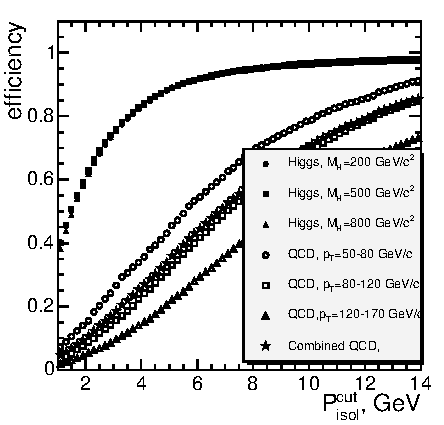
\includegraphics[width=0.55\textwidth]{tau/tautag_ecalisol_hlt}
\caption{The efficiency of the ECAL isolation at the High Level Trigger for 
         the signal and the QCD multi-jet background as a function of the cut 
         $\mathrm{P _{\rm isol}^{\rm cut}}$ on the ECAL isolation parameter.~\cite{CMS_TDR_PHYS_vol1, citeulike:800614} }
\label{fig:tautag_ecalisol_hlt}
\end{figure}

Figure~\ref{fig:tautag_ecalisol_hlt} shows the efficiency of the ECAL isolation criteria for $\tau$ jets and multi-jets. A reduction in the multi-jet rate of $\sim$ 3 was achieved with $\mathrm{P_{isol}^{cut}} = 5 \GeV$.

Jets that passed the calorimeter isolation were passed through tracker isolation with the pixel detector. Track candidates were formed from hit pairs in the first two pixel layers. Quality cuts were applied consistent with a track \PT of 1 \GeVc or above. Hits from the third pixel layer were combined with the track candidates to form pixel-tracks. A list of primary vertices was formed from the pixel-track z impact parameters. Vertices associated with fewer than three pixel-tracks were discarded. Each vertex was computed as the mean of the z impact parameters of the constituent tracks.

The tracker isolation was then run with the pixel-tracks. The lead track was required to have $\mathrm{p_{T}^{ltr}} > 3 \GeVc$ and to be within the cone $\mathrm{R_{m}} = 0.1$ around the jet axis. All further tracks were required to come from the same vertex as the lead track. Signal tracks were located within the cone $\mathrm{R_{S}}$=0.07 with no further tracks permitted within the isolation cone, $\mathrm{R_{i}}$.

\begin{figure}[!hHtb]
\begin{center}
\begin{tabular}{cc}
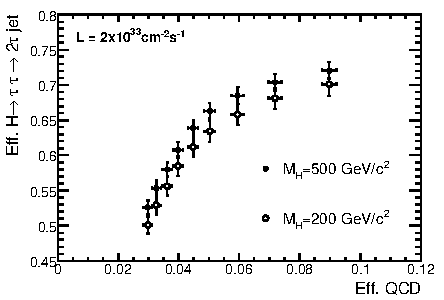
\includegraphics[width=0.49\textwidth]{tau/eff_hlt_pix_1stjet}
&
\includegraphics[width=0.49\textwidth]{tau/eff_hlt_pix_2jets}
\end{tabular}
    \caption{Efficiency of Calo+Pxl trigger applied to the 
             first jet (left) and to both jets (right) for signal 
             events versus efficiency for QCD multi-jet events. 
             Two Higgs boson masses of $\mathrm{M}_{\rm H}$=200 and 
             500 GeV/$c^{2}$ are shown. The isolation cone is varied from 0.2 to 
             0.6 in steps of 0.05; the signal cone is 0.07; the matching cone is 0.1; 
             and the $\PT$ of the leading tracks must exceed 
             3 GeV/$c$.~\cite{CMS_TDR_PHYS_vol1, citeulike:800614} 
}
\label{fig:pxl_eff}
\end{center}
\end{figure}

Figure~\ref{fig:pxl_eff} shows the Calo+Pxl single (left) and double (right) $\tau$ efficiencies for both H$\rightarrow \tau \tau$ and QCD multi-jets (50 $< \ETMC < 170 \GeV$) as a function of the isolation cone size. The A/H$\rightarrow \tau \tau$ analysis required a double trigger. It can be seen that a double trigger background rejection rate of $\sim 10^{-3}$ could be achieved with an $\mathrm{R_{i}}$ of 0.45--0.5, giving a signal efficiency of 0.29--0.32.

\section{$\tau$ jet energy scale}
Figures~\ref{fig:tau_scale} and~\ref{fig:jet_scale} show the $\tau$ and QCD multi-jet energy scales. The drop at $\eta~\simeq 1.4$ was due to the instrumentation gap between the calorimeter barrel and endcap sections. It can be seen that the $\tau$ energy scale was significantly higher than that of multi-jets. This was a consequence of the intrinsically higher electromagnetic response and the $\tau$ jets' low multiplicity. Both these resulted from $\tau$ jets being predominantly light quark jets containing neutral pions. Thus $\tau$ jets required a dedicated energy scale calibration.
%The highest response was from $\tau$ decays involving $\pi^{0}$s and a low number of $\pi^{\pm}$s. This was a consequence of the intrinsically higher electromagnetic response and the $\tau$ jets low multiplicity. Thus $\tau$ jets required a dedicated energy scale calibration.

\begin{figure}[tb]
  \centering
  \includegraphics[width=0.49\textwidth]{tau/tautag_scalei_vs_pt}
  \includegraphics[width=0.49\textwidth]{tau/tautag_scalei_vs_eta}
  \caption{The Monte Carlo $\tau$ jet energy scale for different decay final states.~\cite{CMS_TDR_PHYS_vol1, citeulike:800614} 
  \label{fig:tau_scale}}
\end{figure}

\begin{figure}[!hHtb]
  \centering
  \includegraphics[width=0.49\textwidth]{tau/tautag_scale_vs_pt}
  \includegraphics[width=0.49\textwidth]{tau/tautag_scale_vs_eta}
  \caption{Simulated $\tau$ jet \ET scale before and after Monte Carlo corrections for 1 and 3 pronged $\tau$ jets in the presence of low luminosity pileup.~\cite{CMS_TDR_PHYS_vol1, citeulike:800614}
  \label{fig:tau_scale_corr}}
\end{figure}

\subsection{Monte Carlo calibration~\label{sec:MC_tau_calib}}

%%%%%
% MC calibration method
% plots
% resoloution - compare standard qcd jets
%%%%%

A Monte Carlo $\tau$ jet energy calibration was developed in this study for use in Monte Carlo analyses. This correction was obtained from a parameterisation in $\eta$ and \ET of the ratio $\mathrm{E_{T}^{reco}/E_{T}^{MC}}$ for  Monte Carlo single prong, 3 prong and 1 + 3 pronged decays in the presence of pileup at an instantaneous luminosity of \lowlumi. Figure~\ref{fig:tau_scale_corr} shows the $\tau$ jet energy scale before and after calibration for 1 + 3 pronged $\tau$ jets.



\begin{figure}[tb]
  \centering
  \includegraphics[width=0.65\textwidth]{tau/tau_resol}
  \caption{The calibrated $\tau$ jet \ET resolution in the presence of low luminosity pileup.~\cite{CMS_TDR_PHYS_vol1, citeulike:800614}
  \label{fig:tau_resol}}
\end{figure}

The energy resolution after the correction can be seen in Figure~\ref{fig:tau_resol} and parameterised as:

\begin{equation}
\mathrm{
\frac{\sigma\left(\frac{E_{T}^{corr}}{E_{T}^{MC}}\right)}{\langle\frac{E_{
	      T}^{corr}}{E_{T}^{MC}}\rangle}=\frac{0.883}{\sqrt{E_{T}^{MC}}} \oplus 0.058
}
\end{equation}

for $\tau$ jets with $E_{T}$ between 30 and 300 GeV and pseudorapidity less than 2.3. Figure~\ref{fig:Jet_perf} shows the comparative plot for QCD multi-jets.

\subsection{Proposal for calibration from data}

%%%%%
% gamma + jet calibration
% pass through tau id
% plots
%%%%%



Once CMS begins data taking a calibration from real data will be needed. One proposal for this involved taking Z $\rightarrow \tau \tau \rightarrow l + jet$ events and reconstructing the Z mass peak~\cite{CMS_TDR_PHYS_vol1}. The $\tau$ energy scale could be computed from the well known lepton energy scale and Z mass peak. Disadvantages of this approach included background contamination and the \MET resolution.

Another approach was proposed.~\cite{CMS_TDR_PHYS_vol1, citeulike:800614} and studied here, using $\gamma$ + jet events, which are already planned to be used to calibrate the QCD multi-jet energy scale. It has been proposed that those jets that pass the $\tau$ tagging criteria may have an energy scale similar to that of genuine $\tau$ jets. To evaluate the feasibility of this approach the QCD multi-jets sample was passed through the $\tau$ tagging criteria and the energy scale determined. Jets were reconstructed with cone size 0.4 and passed through both tracker and ECAL isolation. Isolation was performed with parameters $\mathrm{P_{isol}^{cut}}$=5 GeV, $\mathrm{R_{i}}$=0.4, $\mathrm{R_{S}}$=0.07, lead track \PT $>$ 10 \GeVc and with the requirement for 1 or 3 signal tracks. QCD multi-jets that passed all $\tau$ criteria were termed $\tau$ like. 

Figure~\ref{fig:tau_qcd_scale} shows the results. One can see that $\tau$ like jets had a much higher calorimeter response compared to untagged jets. However there was still a 5--10\% systematic offset. This is probably due to the same reasons that give $\tau$ jets there inherently high energy response. It is possible that this difference may be reduced when CMS adopts particle flow algorithms which could be used to select QCD jets that are even more similar to $\tau$ jets than the ones presently selected. If this approach does not provide similar responses an extra correction factor could be applied to the $\tau$-like jet energy scale. However this would introduce new errors and systematics and would therefore be undesirable.

\begin{figure}[tb]
  \centering
  \includegraphics[width=0.45\textwidth]{tau/tautag_calibr_qcd_pt}
  \includegraphics[width=0.45\textwidth]{tau/tautag_calibr_qcd_eta}
  \caption{The energy scale for $\tau$ jets, QCD multi-jets that pass the $\tau$ tagging criteria and jets which do not.~\cite{CMS_TDR_PHYS_vol1, citeulike:800614}
  \label{fig:tau_qcd_scale}}
\end{figure}

\begin{figure}[tb]
  \centering
  \includegraphics[width=0.45\textwidth]{tau/tautag_calibr_qcd_pt_eff}
  \caption{The efficiency for a QCD multi-jet to pass the $\tau$ tagging criteria.~\cite{CMS_TDR_PHYS_vol1, citeulike:800614}
  \label{fig:tau_qcd_eff}}
\end{figure}
The QCD multi-jet miss-tag efficiency as a function of \ET is shown in Figure~\ref{fig:tau_qcd_eff}.

\section{Conclusion}
The $\tau$ tagging and calibration performance are important for a number of physics channels at CMS. Multiple $\tau$ tagging methods have been developed for use in the High Level Trigger and offline analysis. A Monte Carlo jet energy calibration has been developed and a method proposed to obtain the calibration from data.


%Analysis chapter
\chapter{Study of A/H$\rightarrow\tau\tau\rightarrow$two jets}

\section{Introduction}
Discovery of the heavy neutral Higgs boson would be an important verification of the MSSM Higgs sector and hence the MSSM itself. If calculated its mass could be used as part of a global fit to determine all MSSM parameters. 

Negative searches for the Higgsstrahlung process $e^{+}e^{-} \rightarrow Zh/ZH$ and $e^{+}e^{-} \rightarrow Ah/AH$ at LEP2 yielded limits of $m_{h,H}$\,$>$\,93\GeVcc~\cite{Schael:2006cr}. A $\tan{\beta}$ range could only be excluded within the context of a particular MSSM scenario. The \mhmax benchmark scenario, see Section~\ref{sec:mssm} where m$\mathrm{_h \approx 130\GeVcc}$ and $\mathrm{m_A \gg m_h}$, provided the most conservative $\tan{\beta}$ exclusion of 0.7\,$>$\,$\mathrm{\tan{\beta}}$\,$>$\,2.0 for top quark mass ($\mathrm{m_{t}}$)\,=\,174.3\GeVcc~\cite{Schael:2006cr}. The Tevatron placed upper limits on the \plane plane, which are shown together with the LEP2 limits in Figure~\ref{fig:lep_limit}.

\begin{figure}[htb]
\centering
\includegraphics[width=0.47\textwidth]{analysis/matbmax_col}
\includegraphics[width=0.45\textwidth]{analysis/t4l-benchP16}
\caption{LEP2 (left) and Tevatron (right) limits in the $\tan{\beta}$ - $m_{A}$ plane for the $\mhmax$ scenario.~\cite{Schael:2006cr, citeulike:894146}  
\label{fig:lep_limit}}
\end{figure}

\begin{figure}[htb]
\centering
\includegraphics[width=0.55\textwidth]{analysis/hhmasses}
\caption{Masses of the Higgs bosons for two possible values of $\tan{\beta}$ as a function of $m_{A}$ in the \mhmax scenario.~\cite{citeulike:888485}  
\label{fig:Higgs_degenerate}}
\end{figure}

It is common for an MSSM search to be conducted with a set of benchmark parameters. The scenario that provides the most conservative $\tan{\beta}$ reach is the \mhmax scenario. This scenario was described Chapter 7 and occurs when $m_A \gg \mhmax$. In this scenario the light scalar, h, reaches its maximal value of $\sim$\,130\GeVcc and the neutral heavy Higgs bosons, $A$ and $H$, become almost degenerate in mass, this is shown in Figure~\ref{fig:Higgs_degenerate}. The mass difference between the two is within CMS's jet resolution, thus the two signal distributions are combined in searches.

%Due to the enhanced Yukawa coupling to down type fermions previous CMS studies have studied the decays $H/A \rightarrow \mu^{+}\mu^{-}$, $H/A \rightarrow \tau^{+}\tau{-}$ and $H/A \rightarrow b\bar{b}$ for the associated production channel $gg \rightarrow b\bar{b}H/A$~\cite{CMS_TDR_PHYS_vol2}.
%FIXME check all channels in TDR - also ref summary of the CMS potential...

\begin{figure}[!Hhtb]
\centering
\includegraphics[width=0.45\textwidth]{analysis/xslhc-all}
\includegraphics[width=0.45\textwidth]{analysis/bra-mssm}
\caption{Cross section for MSSM Higgs boson production (left) and branching ratio of the $A$ (right) at the LHC for $\tan{\beta}=30$.~\cite{citeulike:888485}  
\label{fig:Higgs_xsection_BR}}
\end{figure}

Figure~\ref{fig:Higgs_xsection_BR} shows the $H/A$ cross-sections and $A$ branching ratio (BR) for the \mhmax scenario with $\tan{\beta} = 30$. Decays to b quarks and $\tau$'s dominate due to the enhanced coupling to heavy down-type quarks, see Table~\ref{tab:MSSMcoupling}. Similar branching ratios are also obtained for the $H$. The dominant decay to b quarks would be difficult to search for with CMS due to the large hadronic background at the LHC. Thus the second most common decay, to 2 $\tau$ leptons, was studied.

%The $\mu$ decays (not shown in plot) were useful for $m_{A} < 300 \GeVcc$. For large values of $m_{A}$ the $\tau$ channel was favoured.

Many $\tau$ decay channels have been studied at CMS~\cite{CMS_TDR_PHYS_vol2} with fully hadronic final states, with $\tau \rightarrow \nu + j$ providing the highest $m_{A}$ reach. This channel relies on the production associated with b quarks~\cite{CMS_TDR_PHYS_vol2, citeulike:903864} (Figure~\ref{fig:feynman}) and uses $\tau$ and b-tagging for event selection. It was decided for this study to investigate the possibility of replacing the b-tagging selection with one based on \MET. With the elimination of b-tagging this analysis was also sensitive to the second most common production mechanism, \ggH (Figure~\ref{fig:feynman}). The study was performed for the three sample values of $m_A$ = 200, 500 and 800 \GeVcc. This analysis is described below and the resulting reach in the \plane plane for the \mhmax scenario presented.

\begin{figure}
	\centering
	\includegraphics[width=0.35\textwidth]{analysis/feynman-associated}
	\includegraphics[width=0.25\textwidth]{analysis/feynman-fusion}
	\caption{Feynman diagrams of the major Higgs production mechanisms studied in this analysis. Gluon-gluon fusion is shown on the left and associated b production on the right.\label{fig:feynman}}
\end{figure}


\section{Signal and background generation}
Until CMS data-taking begins Monte Carlo data has to be used. Events were produced with full detector simulation at an instantaneous luminosity of \lowlumi. Signal events were generated with PYTHIA~\cite{citeulike:903853} procesess 181 (\bbH) and 152 (\ggH) for 3 values of $\mathrm{m_{A}}$: 200, 500 and 800 \GeVcc. Backgrounds included events with $\tau$ jets and those with jets, or electrons, which could be mis-tagged as a $\tau$. PYTHIA-generated backgrounds included QCD multi-jets, \ZTauTau, \Zee, \TopTop, \Wtb\xspace and \Wjet. W bosons in the samples \TopTop, \Wjet\xspace and \Wtb were forced to decay $W \rightarrow \tau\nu$. All $\tau$ decays were forced to hadrons with the TAUOLA package~\cite{citeulike:903857}.

%PT bins etc...

Loose cuts were applied to the background samples at the generator level to avoid generating excess events that would not pass the offline selection. These selections were looser than those used offline. The main requirement was for 2 $\tau$-like jets with generated \PT (\pthat)\,$>$\,50\GeV. A jet was formed with the PYTHIA PYCELL routine and tagged as $\tau$-like if it was within the tracker acceptance, $|\eta|$\,$<$\,2.4, and had at least one stable charged particle with \PT$>$\,30\GeVc. No \PT preselection was applied to the \ZTauTau sample. A cut of $\mathrm{M_{ee}}$\,$>$\,15\GeVcc was applied to the \Zee sample. No preselection was applied to the signal samples. The generated number of events and generator cut efficiency, $\epsilon_{kine}$, for all generated datasets are shown in Table~\ref{table:datasets}.

\begin{table}[htb]
	\centering
\begin{tabular}{|l|c|c|c|c|}
\hline
sample & $\sigma\times$ BR & generated & generated & $\epsilon_{kine}$ \\ 
        & (fb)              & luminosity (\fb) & events & \\ \hline                      
\bbH\,$m_A = 200 \GeVcc$ & - & - & 100K & 1\\ \hline
\bbH\,$m_A = 500 \GeVcc$ & - & - & 100K & 1\\ \hline
\bbH\,$m_A = 800 \GeVcc$ & - & - & 100K & 1\\ \hline
\ggH\,$m_A = 200 \GeVcc$ & - & - & 100K & 1\\ \hline
\ggH\,$m_A = 500 \GeVcc$ & - & - & 100K & 1\\ \hline
\ggH\,$m_A = 800 \GeVcc$ & - & - & 100K & 1\\ \hline
QCD\,$50 < \pthat < 80\GeV$ & $2.11\ten{10}$ & 0.020 & 100K & 2.44\ten{-4} \\ \hline
QCD\,$80 < \pthat < 120\GeV$ & $2.94\ten{9}$ & 0.012 & 200K & 5.77\ten{-3} \\ \hline
QCD\,$120 < \pthat < 170\GeV$ & $5.03\ten{8}$ & 0.009 & 200K & 4.19\ten{-2} \\ \hline
QCD\,$170 \GeV < \pthat$ & $1.33\ten{8}$ & 0.008 & 1000K & 2.12\ten{-1} \\ \hline
\Ztautau\,\ZTauTaua & $1.57\ten{6}$ & 4.3 & 128K & 1.90\ten{-2}\\ \hline
\Ztautau\,\ZTauTaub & $1.24\ten{4}$ & 59 & 70K & 9.53\ten{-2} \\ \hline
\Ztautau\,\ZTauTauc & $6.22\ten{2}$ & 299 & 60K & 3.23\ten{-1} \\ \hline
\Zee & 3.96\ten{6} & 0.24 & 985K & 1\\ \hline
\TopTop & 5.76\ten{3} & 285 & 80K & 4.88\ten{-2}\\ \hline
\Wjet & 5.74\ten{5} & 32 & 400K & 2.16\ten{-2} \\ \hline
\Wtb & 7.10\ten{2} & 3053 & 30K & 1.38\ten{-2}\\ \hline
%$S/\sqrt{B}$ & 6.2 & 7.8 & 5.5 \\ \hline
\end{tabular}
\caption{Generated datasets listing the process cross section, generation cut efficiency, generated events and luminosity. Luminosity and cross sections are not shown for the signal samples as they cannot be calculated without knowledge of the MSSM parameters.  Background cross sections are assumed to have no error. Errors on the number of background events are introduced later for the dominant backgrounds.\label{table:datasets}}
\end{table}

%All samples were produced with full detector simulation at an instantaneous luminosity of \lowlumi.

%\subsection{Kinematics}
%not sure if needed

\section{Level-1 and high level triggers}
The Level-1 $\tau$ trigger was described in Section~\ref{sec:trigger}. Either a single 93\GeV or two 66\GeV $\tau$ triggers were required. These values were optimised for the available trigger bandwidth, 3.2 kHz, as shown in Ref~\cite{CMS_TDR_PHYS_vol1}. The \ET cut was applied after Level-1 jet corrections. These corrections were optimised for non $\tau$ jets and thus over-corrected the $\tau$ \ET. The signal efficiency and purity as a function of $\tau$ \ET can be seen in Figure~\ref{fig:L1_eff_purity}.\footnote{This analysis uses the \ET jet recombination scheme that results in massless jets where \PT is equivalent to \ET.}

\begin{figure}[tb]
\centering
\includegraphics[width=0.49\textwidth]{analysis/L1Tau1Eff_vs_Et}
\includegraphics[width=0.49\textwidth]{analysis/L1Tau1Eff_vs_Eta}
\caption{Level-1 efficiency (ratio of Level-1 to Monte carlo level $\tau$s) and purity of the most energetic $\tau$. A $\tau$ is defined as pure if it is within a distance of 0.4 in R of the true jet.   
\label{fig:L1_eff_purity}}
\end{figure}

The HLT strategy was described in section~\ref{sec:CaloPxl}. The event selection criteria required two HLT $\tau$ candidates with no jet \ET threshold. No \ET threshold was applied as the Level-1 threshold had already been applied and the $\tau$ id criteria resulted in an adequate rate of 4 Hz.

\section{Offline reconstruction and selections}
The offline process included: further $\tau$ identification with tighter cuts: jet calibration and cuts; \MET calibration and cuts; and Higgs boson reconstruction. These cuts were optimised for the greatest 5$\sigma$ discovery reach in the \plane plane for each of the 3 $m_A$ scenarios. 

\subsection{$\tau$ Identification and reconstruction}
The two HLT $\tau$ candidates were reconstructed with the iterative cone algorithm~\cite{CMS_TDR_PHYS_vol1} and cone size 0.4. The algorithm took as input calorimeter towers with thresholds of \ET\,=\,0.5\GeV and E\,=\,0.8\GeV with a 1\GeV seed threshold. These cuts had been optimised to suppress fake jet contamination~\cite{citeulike:903868}. Global track reconstruction was performed with the full tracker and parameters listed in Section~\ref{sec:tracker_isolation}.

%Initial $\tau$ identification was applied with loose cuts which were then individually tightened. Candidates were required to have a lead track within the matching cone, $R_{m} = 0.1$, with $\PT > 10 \GeVc$ 

The following offline $\tau$ id cuts were applied: jet \ET, tracker isolation and electron rejection.

\subsubsection{$\tau$ jet threshold}
$\tau$ jet \ET thresholds were used to reduce the backgrounds. Figure~\ref{fig:tau_max_min} shows the signal \ET distribution. The difference between the \ET of the two $\tau$ jets motivated the use of asymmetric \ET cuts. The least energetic $\tau$ was required to have $\ET > 50 \GeV$ due to the background preselection. The most energetic $\tau$ \ET cut was set to 65, 100 and 130 \GeV for the three $m_{A}$ scenarios. 

\begin{figure}[tb]
\centering
\includegraphics[width=0.45\textwidth]{analysis/TauEt_max_min_200}
\includegraphics[width=0.45\textwidth]{analysis/TauEt_max_min_500}
\includegraphics[width=0.45\textwidth]{analysis/TauEt_max_min_800}
\caption{$E_{T}^{\mathrm{reco}}$ distribution for signal datasets, $m_{A}=200$\GeVcc (left), $m_{A}=500$\GeVcc (right) and $m_{A}=800$\GeVcc (bottom).   
\label{fig:tau_max_min}}
\end{figure}

\subsubsection{Tracker isolation}
Tracks reconstructed with the full tracker were used to recalculate the tracker isolation. The parameters were the same as those at the HLT, with the exceptions $\mathrm{p_{T}^{ltr} > 32 \GeV}$ and $\mathrm{R_{s}=0.04}$. This was done to further reduce the QCD fake rate for this particular analysis. Also a requirement on the number of signal tracks was introduced. The effect of this can be seen in Figure~\ref{fig:sig_cone}, where the number of tracks within the signal cone around the lead track is shown for the main data samples. It can be seen that a requirement for one signal track rejects 60--70\% of the QCD multi-jet background.

\begin{figure}[tb]
\centering
\includegraphics[width=0.45\textwidth]{analysis/TauProngs_200}
\includegraphics[width=0.45\textwidth]{analysis/TauProngs_500}
\includegraphics[width=0.45\textwidth]{analysis/TauProngs_800}
\caption{Signal track distribution for signal, QCD multi-jets, \Ztautau\xspace and other backgrounds for $m_{A}=200$\GeVcc (left), $m_{A}=500$\GeVcc (right) and $m_{A}=800$\GeVcc (bottom).\label{fig:sig_cone}}
\end{figure}

%\begin{table}[tbp]
%	\begin{tabular}{|l|c|c|c|c|}
%	\hline
%	& $m_{A}=200 \GeVcc$ & QCD multi-jets & \Ztautau & S/$\sqrt(\rm B)$ \\ \hline
%	1 or 3 tracks, $R_{s}=0.04$ & 38.1 & 61.8 & 8.5 & 4.5 \\ \hline
%	1 track, $R_{s}=0.04$ & 35.3 & 23.9 & 4.2 & 6.6 \\ \hline
%	1 or 3 tracks, $R_{s}=0.07$ & 38.4 & 109.6 & 8.5 & 2.5 \\ \hline
%	1 track, $R_{s}=0.07$ & 35.3 & 24.0 & 4.2 & 6.6 \\ \hline
 %   \end{tabular}
%\caption{Expected number of events and signal significance within $m_{A}=200\GeVcc$ mass window (defined later) for 60 \fb of data in the \mhmax scenario with $\tan{\beta}=20$.\label{tab:tracks}}
%\end{table} 

\subsubsection{Electron rejection}
To reduce \Zee\xspace contamination a cut on the hottest HCAL tower in the jet was introduced, as described in Section~\ref{sec:e_rejection}. Both $\tau$ jet candidates were required to pass the threshold. Figure~\ref{fig:lowHotHcal} shows the least hot HCAL tower of the two reconstructed $\tau$s in an event. A cut of 1.5 \GeV was sufficient to suppress highly \Zee\xspace.

\begin{figure}[!Hhtb]
\centering
\includegraphics[width=0.45\textwidth]{analysis/lowestHottestHCALtower}
\caption{Distribution of the lowest value of the 2 $\tau$ jets hottest HCAL tower. All samples have passed both trigger levels and the offline tracker isolation.\label{fig:lowHotHcal}}
\end{figure}

Previous studies~\cite{CMS_TDR_PHYS_vol2} have shown further $\tau$ tagging procedures developed at CMS based on impact parameter and the $\tau$ mass did not provide significant improvement after the trigger and offline tracker isolation.

\subsubsection{$\tau$ \ET calibration}
The $\tau$ jets were calibrated with the Monte Carlo jet \ET corrections in Section~\ref{sec:MC_tau_calib}. Figure~\ref{fig:analysis_tau_scale} shows the effect of the correction. The overcorrection in the first \ET bin of the left plot was due to the application of tighter cuts than for the calibration. The overcorrection was not large enough to warrant a new calibration.

\begin{figure}[!Hhtb]
\centering
\includegraphics[width=0.45\textwidth]{analysis/TauEtScale_vs_Et}
\includegraphics[width=0.45\textwidth]{analysis/TauEtScale_vs_Eta}
\caption{$E_{T}$ distribution and calibration for signal events passing cuts $\mathrm{E_{T}^{reco} > 50} \GeV, \mathrm{p_{T}^{ltr}} > 32 \GeVc$.\label{fig:analysis_tau_scale}}
\end{figure}

\subsection{Missing energy}
The \MET for an event was measured by summing all the calorimeter towers and obtaining $\mathrm{E_{x}}$ and $\mathrm{E_{y}}$. True (MC) \MET was calculated by summing all stable Monte Carlo particles except $\nu$ and $\mu$. The true \MET distributions can be seen in Figure~\ref{fig:MET} along with the difference between the true and reconstructed \MET. It can be seen that the detector \MET for the multi-jet background was considerably higher than the true value. This was due to limits on the detector's coverage and the imperfect calorimeter response.

\begin{figure}[!Hhtb]
\centering
\includegraphics[width=0.45\textwidth]{analysis/MCMET_200}
\includegraphics[width=0.45\textwidth]{analysis/MET_profile_200}
\includegraphics[width=0.45\textwidth]{analysis/MCMET_500}
\includegraphics[width=0.45\textwidth]{analysis/MET_profile_500}
\includegraphics[width=0.45\textwidth]{analysis/MCMET_800}
\includegraphics[width=0.45\textwidth]{analysis/MET_profile_800}
\caption{True \MET distribution (left) and difference between true and reconstructed \MET (right) for $m_{A}=200$\GeVcc (top), $m_{A}=500$\GeVcc (middle) and $m_{A}=800$\GeVcc (bottom). The background distributions differ between the $m_A$ plots as different cuts are applied for each scenario.\label{fig:MET}}
\end{figure}

Calibrations for the detector \MET response had been developed~\cite{citeulike:905600}. These corrections involved a global jet reconstruction for jets with \ET\,$>$\,25\GeV. For each jet the constituent towers energy contributions were replaced by that of the jet. The jet energy was calibrated to correct for out-of-cone energy leakage and pileup. The correction may be written:

\begin{equation}
\rm E_{\rm Tx(y)}^{\rm miss}= -(\rm E _{Tx(y)}^{\rm raw}+
                           \sum _{jets} (\rm E _{\rm Tx(y)}^{\rm corr.jet} - \rm E _{\rm Tx(y)}^{\rm raw jet}))
\label{eqn:MET_corr}
\end{equation}

where $\rm E _{Tx(y)}^{\rm raw}, \rm E _{\rm Tx(y)}^{\rm corr.jet} \mathrm{ and }\,\rm E _{\rm Tx(y)}^{\rm raw jet}$ represent the calorimeter response, corrected and uncorrected jet energies, respectively. 

\begin{figure}[!Hhtb]
\centering
\includegraphics[width=0.45\textwidth]{analysis/MET_profile}
\caption{Average difference between reconstructed and true \MET (GeV) in QCD and $gg \rightarrow bbH$ events, both with and without corrections applied.\label{fig:MET_profile}}
\end{figure}

Figure~\ref{fig:MET_profile} shows the effect of the \MET correction. For events with true (MC) $\MET < 40 \GeV$ the correction can be seen to overestimate the \MET of the multi-jet sample while providing a negligible correction to the Higgs events. Thus the correction was only applied to events with $\MET > 40 \GeV$.

The \MET cut was set to 50, 70 and 70\GeV for $m_{A} = 200, 500 \mathrm{\,and\,} 800\GeVcc$, respectively. The $m_{A} = 200 \GeVcc$ cut had a low signal efficiency ($\sim$\,10\%) but was necessary for background suppression.

\subsection{Higgs mass reconstruction}
The undetectable neutrinos required assumptions to be made to allow the Higgs boson mass to be reconstructed. It was assumed that the $\nu$ was emitted collinear with the $\tau$. The corrected \MET could then be projected onto the two jet direction vectors. This then allowed the reconstructed Higgs mass, $\mathrm{M_{\tau \tau}}$, to be derived with:

\begin{equation}
	\mathrm{ M_{\tau \tau} = [2\,E_{\tau 1}\,E_{\tau 2} ( 1 - \cos{\theta_{\tau \tau}})]^{1/2} }
\end{equation}

where $\mathrm{E_{\tau 1},\,E_{\tau 2},\,\cos{\theta_{\tau \tau}}}$ represent the \ET of the two $\tau$s and the angle in $\theta$ between them. 

A number of quality cuts were applied to improve the $M_{\tau\tau}$ resolution. These requirements were positive energy neutrinos and non-back-to-back $\tau$ jets. Figure~\ref{fig:mass_resolution} shows the $M_{\tau\tau}$ distribution as a function of the angle in $\phi$ between the jets, $\Delta \phi_{jj}$, and as each reconstruction cut was applied. The $\Delta \phi_{jj}$ cut was set to 175\de.

\begin{figure}[!Hhtb]
\centering
\includegraphics[width=0.45\textwidth]{analysis/mTauTau_vs_dphiJetJet_scatter_signal}
\includegraphics[width=0.45\textwidth]{analysis/HiggsMass_noQuality_200}
\includegraphics[width=0.45\textwidth]{analysis/HiggsMass_noQuality_500}
\includegraphics[width=0.45\textwidth]{analysis/HiggsMass_noQuality_800}
\caption{$M_{\tau \tau}$ scatter plot (top left) and distribution for $m_{A}$ = 200 (top right), 500 (bottom left) and 800 (bottom right)\GeVcc . The scatter plot is shown before the $\Delta \phi_{jj}$ cut. The distributions show $\mathrm{M_{\tau \tau}}$ before and after the quality cuts. The mass distribution with the $\Delta \phi$ cut has been fitted with a gaussian within the mass window ranges listed in 8.4.3.\label{fig:mass_resolution}}
\end{figure}

A mass window was formed around each $\mathrm{M_{\tau \tau}}$ peak and the number of signal and background events contained within used to calculate the discovery significance. The windows used were 150--250, 400--700 and 600--1100\GeVcc for $m_{A}$ = 200,\,500 and 800\,\GeVcc. Within the mass windows these cuts resulted in mass resolutions of 9.6\%, 16.1\% and 19.2\% for $m_{A}\mathrm{=200, 500\, and\, 800 \GeVcc}$, respectively. 

\section{Cut overview}
Table~\ref{table:cuts} shows a compete list of all cuts used in this analysis. The event kinematics for the different $m_{A}$ scenarios meant that no single set of cut parameters was appropriate for all cases. Thus the cuts were optimised separately for each of the three $m_{A}$ scenarios. The point of lowest 5$\sigma$ discovery in the \plane plane was obtained for each $m_A$ value. The lower this number the greater the area in the \plane plane that could be searched. For the analysis of real data it was assumed that other searches would place limits on the allowed values of $m_{A}$, thus allowing the appropriate cuts to be used. 

Figure~\ref{fig:cut_optimisation} shows the optimisation of individual cuts for $\tan{\beta}$ reach. Cuts were not automatically set to the lowest point for every cut-$m_A$ combination due to complications introduced by the generator level selections and the need for a statistically meaningful sample of passing events. Cuts could not be set below the value used at the generator level, which imposed a lower bound on the cut. As the cuts were increased the amount of signal and background events passing all cuts sharply decreased. Thus the seemingly lowest $\tan{\beta}$ reach could not be relied on as it may not provide a statistically meaningful result. At least 20 events were required to pass in each dataset to allow statistically meaningful conclusions to be drawn. The final cut values taken were the lowest points in Figure~\ref{fig:cut_optimisation} that were greater than the generator level selection whilst still statistically meaningful. 

%The cuts were varied as long as a significant number of events passed all cuts. This was to ensure the results were statistically meaningful. The reach was set to infinity if less than 20 signal events passed all cuts. Note that cuts were not automatically tuned to the lowest point if the background samples did not have a statistically meaningful number of events pass. 


\begin{table}[tb]
\begin{tabular}{|l|c|c|c|}
\hline
	& $m_{A}$ = 200 \GeVcc & $m_{A}$ = 500 \GeVcc & $m_{A}$ = 800 \GeVcc\\ \hline
% 	   & tan($\beta$)=20 &  tan($\beta$)=20 & tan($\beta$)=20 \\ \hline
%	\multicolumn{4}{c}{Trigger selections} \\ \hline
	Level-1 $\tau$ trigger & \multicolumn{3}{|c|}{single $\tau$ \ET = 93 GeV or Double $\tau$ \ET = 66 \GeV} \\ \hline
	HLT CaloPxl & \multicolumn{3}{|c|}{$\mathrm{P_{isol}^{cut}} = 5 \GeV, \mathrm{p_{T}^{ltr}} > 3 \GeVc, \mathrm{R_{m}} = 0.1, \mathrm{R_{S}} = 0.07, \mathrm{R_{i}}=0.5$} \\ \hline
%	\multicolumn{4}{c}{Offline selections} \\ \hline
	2 calorimeter jets &  \multicolumn{3}{|c|}{ $\ET > 10 \GeVcc$} \\ \hline
	\ET cut & 65 and 50\GeV & 100 and 50\GeV & 130 and 50\GeV \\ \hline
	2 offline $\tau$ candidates & \multicolumn{3}{|c|}{$\mathrm{R_{m} = 0.1, p_{T}^{ltr} > 10 \GeV}$} \\ \hline
	Lead track & \multicolumn{3}{|c|}{$\mathrm{p_{T}^{ltr} > 32 \GeV}$} \\ \hline
	Tracker isolation & \multicolumn{3}{|c|}{$\mathrm{R_{i}}=0.5$} \\ \hline
	Signal tracks & \multicolumn{3}{|c|}{1 track within cone $\mathrm{R_{S}} = 0.04$} \\ \hline
	$e^{-}$ rejection & \multicolumn{3}{|c|}{Hottest HCAL tower $>$ 1.5 \GeV} \\ \hline
	Charge correlation & \multicolumn{3}{|c|}{$Q_{\tau_{1}} \times Q_{\tau_{1}} = -1$} \\ \hline
	\MET & $\MET > 50 \GeV$ & $\MET > 70 \GeV$ & $\MET > 70 \GeV$ \\ \hline
%	\multicolumn{4}{c}{$M_{\tau \tau}$ quality selections} \\ \hline
	Positive energy $\nu$ & \multicolumn{3}{|c|}{$\mathrm{E_{\nu 1}, E_{\nu 2} > 0}$} \\ \hline
	Non-back-to-back jets & \multicolumn{3}{|c|}{$\mathrm{\phi_{ j j} < 175\de}$} \\ \hline
	Mass window & 150--250 \GeVcc & 400--700 \GeVcc & 600--1100 \GeVcc \\ \hline
\end{tabular}
\caption{Summary of cuts for each $m_{A}$ scenario.\label{table:cuts}}
\end{table}

\begin{figure}[tb]
\centering
\includegraphics[width=0.45\textwidth]{analysis/OfflineJetEtCut1}
\includegraphics[width=0.45\textwidth]{analysis/OfflineJetEtCut2}
\includegraphics[width=0.45\textwidth]{analysis/OfflineleadTrackPtCut}
\includegraphics[width=0.45\textwidth]{analysis/OfflineMETcut}
\caption{$\tan{\beta}$ reach as a function of cut parameters. Varied cuts are \ET of most energetic $\tau$ ($\mathrm{E_{T}^{\tau 1}}$), \ET of least energetic $\tau$ ($\mathrm{E_{T}^{\tau 1}}$), \PT of $\tau$ lead track ($\mathrm{p_{T}^{ltr}}$) and \MET. Each cut is varied for 3 mass scenarios $m_A$ = 200 (squares), 500 (upward pointing triangles) and 800 (downward pointing triangles)\GeVcc.\label{fig:cut_optimisation}}
\end{figure}

\section{Efficiencies and number of events}
To obtain estimates for the expected number of events a set of MSSM parameters had to be chosen. The \mhmax scenario was used with the paramaters $M_{t} = 175\GeVcc, M_{2} = 200\GeVcc, \mu = 200 \GeVcc, X_{\rm t} = 2000\TeVcc, M_{susy} = 1\TeVcc$. These parameters are suggested in Ref~\cite{citeulike:894146}. These were used with the FeynHiggs~\cite{citeulike:905609} program to obtain cross-sections. Values of $\tan{\beta}$ were set to be close to the expected 5$\sigma$ discovery significance for 60\fb of data for each of the three $m_A$ scenarios. The actual 5$\sigma$ discovery significance is calculated later. The values of $\tan{\beta}$ used were 20, 30 and 40 for $m_A$ = 200, 500 and 800 \GeVcc, respectively. 

The signal and background efficiencies for all datasets except the QCD multijets and \Zee for each $m_{A}$ scenario are shown in Tables~\ref{table:eff_200},\,\ref{table:eff_500} and \ref{table:eff_800}. It was not possible to apply sensible cuts and have a significant number of multi-jet and \Zee events pass all cuts. Thus for these samples the cuts were factorised into three groups, where the first was applied followed independently by the second and third groups. The group efficiencies were combined to form the total efficiency. The first group contained the Level-1 trigger and offline calorimeter reconstruction. The second contained the HLT and offline $\tau$ identification. The third group contained the \MET and $\mathrm{M_{\tau \tau}}$ quality cuts. Due to the low numbers of QCD events the requirement for oppositely charged jets was not enforced for these events. Previous studies~\cite{citeulike:903864} have shown that this results in a 50\% efficiency, so this value was used. Efficiencies for the factorised cuts are shown in Tables~\ref{table:eff_fact_200}, \ref{table:eff_fact_500} and \ref{table:eff_fact_800} for $m_{A} = 200, 500 \mathrm{\,and\,} 800\GeVcc$, respectively. 

\begin{figure}[!tb]
\centering
\includegraphics[width=0.45\textwidth]{analysis/Zee}
\caption{$M_{\tau \tau}$ distributions for \Zee with and without factorised cut groups. Obtained with relaxed cuts: \ET $>$ 30 \GeV, $\mathrm{p_{T}^{ltr} > 10 \GeV}$, \MET $>$ 10 \GeV and hot HCAL tower $>$ 0.5 \GeV.\label{fig:zee_factorised}}
\end{figure}

The cut factorisation was not applied to all samples as the cut groups were not independent for samples containing genuine $\tau$ jets. The $\mathrm{M_{\tau \tau}}$ distribution obtained with relaxed cuts for \Zee, with and without factorised cut groups, is shown in Figure~\ref{fig:zee_factorised}. The two distributions were compared with the Kolmogorov test and a similarity of 27.8\% obtained. It can be seen that the factorised cuts resulted in an over-estimation of the distribution. As the factorisation was only applied to background datasets this resulted in a higher background than would otherwise be expected. Thus results obtained represented a worst case scenario. A comparison of the multi-jets was not performed as not enough Monte Carlo events passed all cuts even when they were relaxed.

Some data samples that had been generated in multiple \ET/mass ranges had no events in a set range that passed all cuts. This was because they fell outside of the signal region, i.e. their generated \ET was below the cut or their invariant mass was outside the mass window.

The \TopTop, \Wjet\,and some QCD multi-jet datasets ran out of events before passing all selections in certain $m_{A}$ scenarios. Factorised cuts could not be used for the \Wjet\xspace or \TopTop\xspace  samples as they contained genuine $\tau$ jets. In these cases the cuts were loosened until a significant number of Monte Carlo events passed. These were then used to obtain a prediction for the upper bound on the expected number of background events.

\begin{figure}[!Hhtb]
\centering
\includegraphics[width=0.45\textwidth]{analysis/HiggsMass_200}
\includegraphics[width=0.45\textwidth]{analysis/HiggsMass_500}
\includegraphics[width=0.45\textwidth]{analysis/HiggsMass_800}
\caption{$M_{\tau \tau}$ distributions for expected signal and background for $m_{A} = 200,\,500\, \mathrm{and}\,800\GeVcc$ in the \mhmax scenario with $\tan{\beta}$ = 20, 30 and 40 scaled for 60 \fb of data.\label{fig:mass_plots}}
\end{figure}

\begin{sidewaystable}
	\centering
	  \begin{tabular}{|l|c|c|c|c|c|c|c|c|}
  \hline
& $ \bbH $
& $ \ggH $
& $ \TopTop $
& $ \Wjet $
& $ \Wtb $
& $ \ZTauTau$
& $ \ZTauTau$
& $ \ZTauTau$
\\
& & & & &  & \ZTauTaua & \ZTauTaub & \ZTauTauc
\\ \hline
$\sigma \times BR \times \epsilon_{kine}$ & 3753 & 476 & 281 & 12398 & 9.8 & 29830 & 1182 & 201 \\ \hline
L1 $\tau$ Trigger & 0.501 & 0.519 & 0.753 & 0.784 & 0.826 & 0.530 & 0.702 & 0.859 \\ \hline
HLT CaloPxl & 0.291 & 0.246 & 0.047 & 0.034 & 0.128 & 0.046 & 0.192 & 0.241 \\ \hline
2 offline calorimeter $\tau$ jets & 0.997 & 0.998 & 0.994 & 0.995 & 0.997 & 0.984 & 0.999 & 0.999 \\ \hline
$\tau E_{T}^{cut}$ & 0.347 & 0.348 & 0.562 & 0.725 & 0.585 & 0.241 & 0.415 & 0.842 \\ \hline
2 offline $\tau$ candidates & 0.678 & 0.688 & 0.815 & 0.800 & 0.795 & 0.693 & 0.699 & 0.713 \\ \hline
$\mathrm{p_{T}^{ltr}}$ cut & 0.404 & 0.403 & 0.661 & 0.639 & 0.749 & 0.290 & 0.410 & 0.600 \\ \hline
Tracker isolation & 0.855 & 0.854 & 0.825 & 0.476 & 0.852 & 0.638 & 0.850 & 0.918 \\ \hline
Signal tracks & 0.592 & 0.587 & 0.567 & 0.254 & 0.544 & 0.378 & 0.580 & 0.643 \\ \hline
Hottest HCAL Tower & 0.954 & 0.989 & 0.903 & 0.965 & 0.921 & 0.941 & 0.904 & 0.877 \\ \hline
$\mathrm{Q_{\tau 1} x Q_{\tau 2}}$ = -1 & 0.979 & 0.962 & 0.958 & 0.835 & 0.940 & 0.594 & 0.950 & 0.943 \\ \hline
\MET & 0.088 & 0.128 & 0.607 & 0.295 & 0.472 & 0.158 & 0.129 & 0.443 \\ \hline
$\mathrm{E_{\nu 1}, E_{\nu 2}} >$ 0 & 0.298 & 0.507 & 0.426 & 0.138 & 0.383 & 0.333 & 0.475 & 0.470 \\ \hline
$\mathrm{\phi_{j j} < 175\de}$ & 0.824 & 0.882 & 0.867 & 0.467 & 0.861 & 1.000 & 0.679 & 0.502 \\ \hline
Mass window efficiencies&  1.21 \ten{-4}  & 2.77 \ten{-4} &  0.000  &  0.000  &  6.67 \ten{-5} &  0.000  &  5.9 \ten{-5} &  0.000  \\ \hline
Mass window $\sigma (\fbplus)$ &  0.454  &  0.133  &  0.000  &  0.000  &  6.53\ten{-4} &  0.000  &  0.0695  &  0.000  \\ \hline
expected events for 60 $(\fb)$ &  27.3  &  7.94  &  0.000  &  0.000  &  0.0391  &  0.000  &  4.17  &  0.000  \\ \hline
\end{tabular}

	\caption{Efficiencies for signal and background events in the $m_{A} = 200 \GeV$ scenario. $\mathrm{M_{Z}}$ in \GeVcc\label{table:eff_200}}
\end{sidewaystable}

\begin{sidewaystable}
	\centering
	  \begin{tabular}{|l|c|c|c|c|c|}
  \hline
& $ \QCD$
& $ \QCD$
& $ \QCD$
& $ \QCD$
& $ \Zee $
\\
& $ 50 < \pthat < 80\GeV$ & $80 < \pthat < 120\GeV$ & $120 < \pthat < 170\GeV$ & $\pthat > 170\GeV$ &
\\ \hline
$\sigma \times BR \times \epsilon_{kine}$ & 5.08 \ten{6} & 1.70 \ten{7} & 2.11 \ten{7} & 2.82 \ten{7} & 3.97 \ten{6} \\ \hline
L1 $\tau$ Trigger & 0.461 & 0.716 & 0.727 & 0.562 & 0.106 \\ \hline
2 offline calorimeter $\tau$ jets & 0.995 & 0.982 & 0.976 & 0.976 & 0.995 \\ \hline
$\tau E_{T}^{cut}$ & 0.121 & 0.665 & 0.784 & 0.742 & 0.060 \\ \hline
Group 1 cuts &  0.0551 &  0.462  &  0.544  &  0.393  &  0.00622  \\ \hline
HLT CaloPxl & 0.012 & 0.005 & 0.002 & 0.001 & 0.133 \\ \hline
2 offline $\tau$ candidates & 0.879 & 0.839 & 0.860 & 0.830 & 0.554 \\ \hline
$\mathrm{p_{T}^{ltr}}$ cut & 0.608 & 0.647 & 0.569 & 0.547 & 0.741 \\ \hline
Tracker isolation & 0.323 & 0.244 & 0.264 & 0.216 & 0.907 \\ \hline
Signal tracks & 0.100 & 0.216 & 0.250 & 0.067 & 0.937 \\ \hline
Hottest HCAL Tower & 1.000 & 1.000 & 1.000 & 1.000 & 0.007 \\ \hline
$\mathrm{Q_{\tau 1} x Q_{\tau 2}}$ = -1 & 0.500 & 0.500 & 0.500 & 0.500 & 1.00 \\ \hline
Group 2 cuts &  2.00\ten{-3} &  1.32\ten{-3} & 5.75 \ten{-5} & 5.21 \ten{6} &  3.26\ten{-3}  \\ \hline
\MET & 0.006 & 0.008 & 0.024 & 0.086 & 0.047 \\ \hline
$\mathrm{E_{\nu 1}, E_{\nu 2}} >$ 0 & 0.448 & 0.474 & 0.430 & 0.482 & 0.502 \\ \hline
$\mathrm{\phi_{j j} < 175\de}$ & 0.462 & 0.720 & 0.684 & 0.741 & 0.842 \\ \hline
Group 3 cuts &  0.00120  &  0.00264  &  0.00712  &  0.0308  &  0.0201  \\ \hline
Mass window efficiencies &  0.000  &  7.75 \ten{-9}  &  8.26 \ten{-9}  & 3.34 \ten{-9}  &  1.99 \ten{-9}  \\ \hline
Mass window $\sigma (\fbplus)$ &  0.000  &  0.132  &  0.174  &  0.0943  &  0.00789  \\ \hline
expected events for 60 $(\fb)$ &  0.000  &  7.89  &  10.4  &  5.66  &  0.473  \\ \hline
\end{tabular}

	\caption{Efficiencies for factorised background events in the $m_{A} = 200 \GeV$ scenario\label{table:eff_fact_200}}
\end{sidewaystable}

\begin{sidewaystable}
	\centering
	  \begin{tabular}{|l|c|c|c|c|c|c|c|c|}
  \hline
& $ \bbH $
& $ \ggH $
& $ \TopTop $
& $ \Wjet $
& $ \Wtb $
& $ \ZTauTau$
& $ \ZTauTau$
& $ \ZTauTau$
\\
& & & & &  & \ZTauTaua & \ZTauTaub & \ZTauTauc
\\ \hline
$\sigma \times BR \times \epsilon_{kine}$ & 186 & 6.31 & 281 & 12398 & 9.80 & 29830 & 1181 & 201 \\ \hline
L1 $\tau$ Trigger & 0.853 & 0.858 & 0.753 & 0.784 & 0.826 & 0.530 & 0.702 & 0.859 \\ \hline
HLT CaloPxl & 0.322 & 0.267 & 0.047 & 0.034 & 0.128 & 0.046 & 0.192 & 0.241 \\ \hline
2 offline calorimeter $\tau$ jets & 0.999 & 0.999 & 0.994 & 0.995 & 0.997 & 0.984 & 0.999 & 0.999 \\ \hline
$\tau E_{T}^{cut}$ & 0.756 & 0.753 & 0.270 & 0.349 & 0.287 & 0.073 & 0.097 & 0.639 \\ \hline
2 offline $\tau$ candidates & 0.717 & 0.710 & 0.816 & 0.812 & 0.778 & 0.737 & 0.725 & 0.717 \\ \hline
$\mathrm{p_{T}^{ltr}}$ cut & 0.662 & 0.659 & 0.671 & 0.667 & 0.776 & 0.459 & 0.505 & 0.634 \\ \hline
Tracker isolation & 0.950 & 0.942 & 0.845 & 0.486 & 0.852 & 0.583 & 0.840 & 0.922 \\ \hline
Signal tracks & 0.671 & 0.662 & 0.570 & 0.211 & 0.538 & 0.286 & 0.562 & 0.653 \\ \hline
Hottest HCAL Tower & 0.984 & 0.976 & 0.904 & 0.945 & 0.927 & 1.000 & 0.902 & 0.881 \\ \hline
$\mathrm{Q_{\tau 1} x Q_{\tau 2}}$ = -1 & 0.937 & 0.947 & 0.935 & 0.824 & 0.922 & 0.583 & 0.942 & 0.941 \\ \hline
\MET & 0.385 & 0.436 & 0.462 & 0.290 & 0.406 & 0.143 & 0.115 & 0.327 \\ \hline
$\mathrm{E_{\nu 1}, E_{\nu 2}} >$ 0 & 0.428 & 0.529 & 0.452 & 0.133 & 0.372 & 0.000 & 0.333 & 0.477 \\ \hline
$\mathrm{\phi_{j j} < 175\de}$ & 0.523 & 0.753 & 0.848 & 0.500 & 0.812 & 0.000 & 0.800 & 0.527 \\ \hline
Mass window efficiencies&  0.004  &  6.76\ten{-4}  &  1.15\ten{-4} &  5.04\ten {-6} &  5.33\ten{-4} &  0.000  &  0.000  &  0.00125  \\ \hline
Mass window $\sigma (\fbplus)$ &  0.745  &  0.0426  &  0.0324  &  0.0625  &  0.00523  &  0.000  &  0.000  &  0.252  \\ \hline
expected events for 60 $(\fb)$ &  44.7  &  2.56  &  1.95  &  3.75  &  0.313  &  0.000  &  0.000  & 15.1  \\ \hline
\end{tabular}

	\caption{Efficiencies for signal and background events in the $m_{A} = 500 \GeV$ scenario. $\mathrm{M_{Z}}$ in \GeVcc\label{table:eff_500}}
\end{sidewaystable}

\begin{sidewaystable}
	\centering
	  \begin{tabular}{|l|c|c|c|c|c|}
  \hline
& $ \QCD$
& $ \QCD$
& $ \QCD$
& $ \QCD$
& $ \Zee$
\\
& $ 50 < \pthat < 80\GeV$ & $80 < \pthat < 120\GeV$ & $120 < \pthat < 170\GeV$ & $\pthat > 170\GeV$ &
\\ \hline
$\sigma \times BR \times \epsilon_{kine}$ & 5.08 \ten{6} & 1.70 \ten{7} & 2.11 \ten{7} & 2.82 \ten{7} & 3.97 \ten{6} \\ \hline
L1 $\tau$ Trigger & 0.461 & 0.716 & 0.727 & 0.562 & 0.106 \\ \hline
2 offline calorimeter $\tau$ jets & 0.995 & 0.982 & 0.976 & 0.976 & 0.995 \\ \hline
$\tau E_{T}^{cut}$ & 0.001 & 0.061 & 0.467 & 0.667 & 0.020 \\ \hline
Group 1 cuts &  4.61\ten{-4} & 0.0421  &  0.324  &  0.354  &  0.00205  \\ \hline
HLT CaloPxl & 0.024 & 0.004 & 0.002 & 0.001 & 0.112 \\ \hline
2 offline $\tau$ candidates & 1.000 & 0.903 & 0.848 & 0.838 & 0.623 \\ \hline
$\mathrm{p_{T}^{ltr}}$ cut & 0.000 & 0.679 & 0.571 & 0.564 & 0.768 \\ \hline
Tracker isolation & 0.000 & 0.158 & 0.234 & 0.195 & 0.890 \\ \hline
Signal tracks & 0.000 & 0.667 & 0.200 & 0.040 & 0.897 \\ \hline
Hottest HCAL Tower & 0.000 & 1.000 & 1.000 & 1.000 & 0.011 \\ \hline
$\mathrm{Q_{\tau 1} x Q_{\tau 2}}$ = -1 & 0.000 & 0.500 & 0.500 & 0.500 & 1.00 \\ \hline
Group 2 cuts &  0.000  &  2.65\ten{-4} &  4.83 \ten{-5} &  2.90 \ten{-6}  & 4.93\ten{-3} \\ \hline
\MET & 0.024 & 0.001 & 0.004 & 0.034 & 0.022 \\ \hline
$\mathrm{E_{\nu 1}, E_{\nu 2}} >$ 0 & 1.000 & 0.556 & 0.535 & 0.555 & 0.523 \\ \hline
$\mathrm{\phi_{j j} < 175\de}$ & 0.000 & 0.800 & 0.809 & 0.819 & 0.783 \\ \hline
Group 3 cuts &  0.000  &  5.29\ten{-4} &  0.00177  &  0.0155  &  0.00888  \\ \hline
Mass window efficiencies &  0.000  &  7.37 \ten{-10}  &  6.81 \ten{-9}  &  2.61 \ten{-9}  &  5.01 \ten{-9}  \\ \hline
Mass window $\sigma (\fbplus)$ &  0.000  &  0.0125  &  0.144  &  0.0736  &  0.0199  \\ \hline
expected events for 60 $(\fb)$ &  0.000  &  0.750  &  8.61  &  4.42  &  1.19  \\ \hline
\end{tabular}

	\caption{Efficiencies for factorised background events in the $m_{A} = 500 \GeV$ scenario\label{table:eff_fact_500}}
\end{sidewaystable}

\begin{sidewaystable}
	\centering
	  \begin{tabular}{|l|c|c|c|c|c|c|c|c|}
  \hline
& $ \bbH$
& $ \ggH$
& $ \TopTop$
& $ \Wjet$
& $ \Wtb$
& $ \ZTauTau$
& $ \ZTauTau$
& $ \ZTauTau$
\\
& & & & &  &\ZTauTaua&\ZTauTaub&\ZTauTauc\\ \hline
$\sigma \times BR \times \epsilon_{kine}$ & 49 & 0.722 & 281 & 12398 & 9.80 & 29830 & 1181 & 200 \\ \hline
L1 $\tau$ Trigger & 0.896 & 0.875 & 0.753 & 0.784 & 0.826 & 0.530 & 0.702 & 0.859 \\ \hline
HLT CaloPxl & 0.316 & 0.247 & 0.047 & 0.034 & 0.128 & 0.046 & 0.192 & 0.241 \\ \hline
2 offline calorimeter $\tau$ jets & 1.000 & 0.999 & 0.994 & 0.995 & 0.997 & 0.984 & 0.999 & 0.999 \\ \hline
$\tau E_{T}^{cut}$ & 0.832 & 0.782 & 0.121 & 0.170 & 0.132 & 0.027 & 0.019 & 0.411 \\ \hline
2 offline $\tau$ candidates & 0.679 & 0.679 & 0.796 & 0.813 & 0.787 & 0.722 & 0.762 & 0.720 \\ \hline
$\mathrm{p_{T}^{ltr}}$ cut & 0.746 & 0.743 & 0.688 & 0.694 & 0.782 & 0.421 & 0.557 & 0.663 \\ \hline
Tracker isolation & 0.951 & 0.948 & 0.845 & 0.500 & 0.858 & 0.667 & 0.795 & 0.930 \\ \hline
Signal tracks & 0.785 & 0.774 & 0.653 & 0.185 & 0.661 & 0.062 & 0.586 & 0.675 \\ \hline
Hottest HCAL Tower & 0.983 & 0.984 & 0.948 & 0.967 & 0.917 & 1.000 & 0.882 & 0.874 \\ \hline
$\mathrm{Q_{\tau 1} x Q_{\tau 2}}$ = -1 & 0.936 & 0.941 & 0.945 & 0.795 & 0.924 & 0.000 & 0.900 & 0.940 \\ \hline
\MET & 0.568 & 0.601 & 0.477 & 0.543 & 0.475 & 0.000 & 0.407 & 0.400 \\ \hline
$\mathrm{E_{\nu 1}, E_{\nu 2}} >$ 0 & 0.468 & 0.553 & 0.366 & 0.132 & 0.328 & 0.000 & 0.364 & 0.450 \\ \hline
$\mathrm{\phi_{j j} < 175\de}$ & 0.452 & 0.664 & 0.800 & 0.400 & 0.789 & 0.000 & 0.750 & 0.498 \\ \hline
Mass window efficiencies &  0.00827 &  0.0108 &  8.97\ten{-5} &  2.52\ten{-6} & 2.66\ten{-4} &  0.000 &  0.000 &  7.00\ten{-4} \\ \hline
Mass window $\sigma (\fbplus)$ &  0.405 &  0.00783 &  0.0252 &  0.0312 &  0.00261 &  0.000 &  0.000 &  0.141 \\ \hline
expected events for 60 (\fb) &  24.3 &  0.470 &  1.51 &  1.87 &  0.157 &  0.000 &  0.000 &  8.44 \\ \hline
\end{tabular}

	\caption{Efficiencies for signal and background events in the $m_{A} = 800 \GeV$ scenario. $\mathrm{M_{Z}}$ in \GeVcc\label{table:eff_800}}
\end{sidewaystable}

\begin{sidewaystable}
	\centering
	  \begin{tabular}{|l|c|c|c|c|c|}
  \hline
& $ \QCD$
& $ \QCD$
& $ \QCD$
& $ \QCD$
& $ \Zee $
\\
& $ 50 < \pthat < 80\GeV$ & $80 < \pthat < 120\GeV$ & $120 < \pthat < 170\GeV$ & $\pthat > 170\GeV$ &
\\ \hline
$\sigma \times BR \times \epsilon_{kine}$ & 5.08 \ten{6} & 1.70 \ten{7} & 2.11 \ten{7} & 2.82 \ten{7} & 3.97 \ten{6} \\ \hline
L1 $\tau$ Trigger & 0.461 & 0.716 & 0.727 & 0.562 & 0.106 \\ \hline
2 offline calorimeter $\tau$ jets & 0.995 & 0.982 & 0.976 & 0.976 & 0.995 \\ \hline
$\tau E_{T}^{cut}$ &  9.68 \ten{-5}  & 0.003 & 0.099 & 0.536 & 0.007 \\ \hline
Group 1 cuts &  4.39 \ten{-5}  &  0.00231  &  0.0689  &  0.285  &  0.000765  \\ \hline
HLT CaloPxl & 0.000 & 0.007 & 0.002 & 0.001 & 0.101 \\ \hline
2 offline $\tau$ candidates & 0.000 & 0.667 & 0.862 & 0.811 & 0.618 \\ \hline
$\mathrm{p_{T}^{ltr}}$ cut & 0.000 & 0.500 & 0.640 & 0.574 & 0.872 \\ \hline
Tracker isolation & 0.000 & 0.000 & 0.125 & 0.218 & 0.902 \\ \hline
Signal tracks & 0.000 & 0.000 & 0.000 & 0.045 & 0.865 \\ \hline
Hottest HCAL Tower & 0.000 & 0.000 & 0.000 & 1.000 & 0.031 \\ \hline
$\mathrm{Q_{\tau 1} x Q_{\tau 2}}$ = -1 & 0.000 & 0.500 & 0.500 & 0.500 & 1.00 \\ \hline
Group 2 cuts &  0.000  &  0.000  &  0.000  &  3.61 \ten{-6}  &  0.00133  \\ \hline
\MET & 0.000 & 0.000 & 0.008 & 0.033 & 0.038 \\ \hline
$\mathrm{E_{\nu 1}, E_{\nu 2}} >$ 0 & 0.000 & 0.000 & 0.535 & 0.542 & 0.483 \\ \hline
$\mathrm{\phi_{j j} < 175\de}$ & 0.000 & 0.000 & 0.759 & 0.786 & 0.714 \\ \hline
Group3 cuts &  0.000  &  0.000  &  0.00311  &  0.0139  &  0.0133  \\ \hline
Mass window efficiencies &  0.000 &  0.000 & 0.000 &  2.35 \ten{-9} &  6.73 \ten{-9} \\ \hline
Mass window $\sigma (\fbplus)$ & 0.000 &  0.000 &  0.000 &  0.0661 &  0.0267 \\ \hline
expected events for 60 (\fb) &  0.000 &  0.000 &  0.000 &  3.97 &  1.60 \\ \hline
\end{tabular}

	\caption{Efficiencies for factorised background events in the $m_{A} = 800 \GeV$ scenario\label{table:eff_fact_800}}
\end{sidewaystable}

Figure~\ref{fig:mass_plots} shows the $\mathrm{M}_{\tau \tau}$ plots for all $m_{A}$ scenarios. The expected number of signal and background events and the discovery significance can be seen in Table~\ref{table:events}. It can be seen that the major background processes were QCD multi-jets and \Ztautau.

\begin{table}[!Hhtb]
	\centering
\begin{tabular}{|l|c|c|c|}
\hline
process & \multicolumn{3}{|c|}{$m_{A}$ (\GeVcc)} \\ \hline
 & 200  & 500 & 800\\ \hline
\bbH & 27.3 & 44.7 & 24.3\\ \hline
\ggH & 7.9 & 2.6 & 0.47\\ \hline
QCD multijets & $< 25.6$  & 13.8 & $< 6.7$\\ \hline
\Ztautau & 4.2 & 15.1 & 8.4\\ \hline
\Zee & 0.5 & 1.2 & 1.6\\ \hline
\TopTop  & $< 0.43$ & 1.9 & 1.5\\ \hline
\Wjet & $< 1.87$ & 3.7 & 1.9\\ \hline
\Wtb & 0.04 & 0.31 & 0.16\\ \hline
$S/\sqrt{B}$ & 6.2 & 7.8 & 5.5 \\ \hline
\end{tabular}
\caption{Summary of expected events for all 3 mass scenarios for 60\fb in the \mhmax scenario.\label{table:events}}
\end{table}

\section{Evaluation of background from data and systematics}
The background uncertainty was calculated for the two main backgrounds, QCD multi-jets and \Ztautau. 

\subsection{QCD multi-jets}
The QCD multi-jet background could be directly measured from the data by replacing the requirement for jets of opposite electric charge with one for same sign jets. This requirement effectively suppressed all other signal and backgrounds. The number of same sign and opposite sign QCD multi-jet events was equal so a direct measurement of the uncertainty on the number of events was possible. Expected number of events was calculated with all cuts except the mass window. The expected events were 296.5, 34.0, and 8.6 for $m_{A}$ = 200, 500 and 800\GeVcc respectively, giving uncertainties of 5.8, 17.2 and 34.2\%.

\subsection{\Ztautau}
It was not possible to isolate the \Ztautau\xspace background hence the uncertainty on the number of events had to be computed. The total uncertainty, $\mathrm{\Delta_{Z_{\tau \tau}}}$, could be computed:

\begin{equation}
	\mathrm{\Delta_{Z_{\tau \tau}}} = \Delta_{theory} \oplus \Delta_{L} \oplus \Delta_{\epsilon}
\end{equation}

with the terms on the right-hand side representing the uncertainties on the theory (cross section and branching ratio), LHC luminosity and experimental efficiency, respectively. The uncertainty on the $\mathrm{Z \rightarrow \tau \tau}$ branching ratio was small ($\simeq$ 0.1\%) and hence neglected~\cite{pdg2006}. $\Delta_{theory} = 3\%$ was taken from the uncertainty on the cross section~\cite{citeulike:891490}. The nominal CMS value for $\Delta_{L}$ was 3\% for 30 \fb of data and above~\cite{CMS_TDR_PHYS_vol2}.

The experimental selection uncertainty could be computed:

\begin{equation}
	\Delta_{\epsilon} = \Delta_{jet\,scale} \oplus \Delta_{MET} \oplus \Delta_{\tau\,tagging}
\end{equation}

where the energy terms on the right-hand side represent the uncertainty of the experimental selection due to the jet scale, \MET scale and $\tau$ tagging, respectively. The $\tau$ tagging efficiency was calculated as 8.8\% for each $\tau$~\cite{citeulike:905602}. 

\subsubsection{Jet scale}
CMS has calculated that, with 30\,\fb of data or more, the CMS jet scale uncertainty will be 3\% and the calorimeter scale 10\%~\cite{CMS_TDR_PHYS_vol2}. No study of the $\tau$ jet scale systematics had been performed to date so the standard jet uncertainty was used for both $\tau$ and multi-jets. The effect of the jet scale uncertainty is shown in Table~\ref{tab:jetScale}.

\begin{table}[!Hh]
	\centering
	\begin{tabular}{|c|c|c|c|c|c|}
	\hline
	$m_{A}$ scenario & $\epsilon_{0}$ & $\epsilon_{-}$ & $\epsilon_{+}$ & $\epsilon_{+} - \epsilon_{-}$ & \% variation\\ \hline
	200\GeVcc & 0.000324 & 0.000309 & 0.000353 & 0.0000221 & 6.18\\ \hline
	500\GeVcc & 0.00245 & 0.00233 & 0.00258 & 0.000125 & 5.10\\ \hline
	800\GeVcc & 0.00167 & 0.00155 & 0.00178 & 0.000117 & 7.00\\ \hline
    \end{tabular}
\caption{$\Ztautau$ efficiency for 3 different jet scale scenarios. Scenarios are nominal jet scale $\epsilon_{0}$ and $\pm3\%$ ($\epsilon_{\pm}$) variation.\label{tab:jetScale}}
\end{table}

\subsubsection{\MET scale}
$\Delta_{MET}$ was calculated for the corrected \MET as shown in Equation~\ref{eqn:MET_corr}. The equation may be rewritten to separate the terms dependent on the two calorimeter scale uncertainties: 

\begin{equation}
\rm E _{\rm Tx(y)}^{miss}= -([\rm E _{Tx(y)}^{\rm raw}-
                           \sum  _{jets}\rm E _{\rm Tx(y)}^{\rm raw jet}] _{\rm low~\rm E _{\rm T}} +
                           [\sum _{jets}\rm E _{\rm Tx(y)}^{\rm corr.jet}] _{\rm high~E _{\rm T}})
\end{equation}

The calorimeter and jet scale variations were applied independently and the maximal deviations measured. Results for the various $m_{A}$ scenarios are shown in Tables~\ref{tab:metScale200}, \ref{tab:metScale500} and \ref{tab:metScale800}.

\begin{table}[!Hh]
	\centering
	\begin{tabular}{|c|c|c|c|c|}
	\hline
	Calorimeter scale variation & jet scale variation & $\epsilon$ \\ \hline
	1.0   &  1.0  &   0.000324 \\ \hline
	1.1   &  1.03 &   0.000353 \\ \hline
	1.1   &  0.97 &   0.000338 \\ \hline
	0.9   &  1.03 &   0.000309 \\ \hline
	0.9   &  0.97 &   0.000294 \\ \hline
	\multicolumn{2}{|c|}{Maximal variation} & 9.09 \% \\ \hline          
    \end{tabular}
\caption{$\Ztautau$ \MET efficiency for various calorimeter and jet scale variations in the $m_{A} = 200 \GeVcc$ scenario.\label{tab:metScale200}}
\end{table}

\begin{table}[!Hh]
	\centering
	\begin{tabular}{|c|c|c|c|c|}
	\hline
	Calorimeter scale variation & jet scale variation & $\epsilon$ \\ \hline
	1.0   &  1.0  &   0.00245 \\ \hline
	1.1   &  1.03  &  0.00272 \\ \hline
	1.1   &  0.97  &  0.00275 \\ \hline
	0.9   &  1.03  &  0.00232 \\ \hline
	0.9   &  0.97  &  0.00232 \\ \hline
	\multicolumn{2}{|c|}{Maximal range} & 8.84 \% \\ \hline          
    \end{tabular}
\caption{$\Ztautau$ \MET efficiency for various calorimeter and jet scale variations in the $m_{A} = 500 \GeVcc$ scenario.\label{tab:metScale500}}
\end{table}

\begin{table}[!Hh]
	\centering
	\begin{tabular}{|c|c|c|c|c|}
	\hline
	Calorimeter scale variation & jet scale variation & $\epsilon$ \\ \hline
	1.0   &  1.0   &  0.00167 \\ \hline
	1.1   &  1.03  &  0.00183 \\ \hline
	1.1   &  0.97  &  0.00173 \\ \hline
	0.9   &  1.03  &  0.00157 \\ \hline
	0.9   &  0.97  &  0.00153 \\ \hline
	\multicolumn{2}{|c|}{Maximal range} & 9.00 \% \\ \hline          
    \end{tabular}
\caption{$\Ztautau$ \MET efficiency for various calorimeter and jet scale variations in the $m_{A} = 800 \GeVcc$ scenario.\label{tab:metScale800}}
\end{table}
\newpage
\subsubsection{Total \Ztautau\xspace uncertainty}
The \Ztautau\,background uncertainty constituents were combined and the final values computed are shown in Table~\ref{tab:zUncertain}.

\begin{table}[!Hh]
	\centering
	\begin{tabular}{|c|c|c|c|c|c|c|}
	\hline
	$m_{A} (\GeVcc)$ & $\Delta_{theory}$ & $\Delta_{L}$ & $\Delta_{jet scale}$ & $\Delta_{MET}$ & $\Delta_{\tau tagging}$ & $\Delta_{Z_{\tau \tau}}$ \\ \hline
	200 & 0.03 & 0.03 & 0.0618 & 0.0909 & 2 $\times$ 0.088 & 0.166 \\ \hline
	500 & 0.03 & 0.03 & 0.0510 & 0.0884 & 2 $\times$ 0.088 & 0.158 \\ \hline
	800 & 0.03 & 0.03 & 0.07 & 0.09 & 2 $\times$ 0.088 & 0.166 \\ \hline 
    \end{tabular}
\caption{\Ztautau\xspace background uncertainty for $m_{A} = 200, 500 \mathrm{\,and\,} 800 \GeVcc$.\label{tab:zUncertain}}
\end{table}

\subsection{Total uncertainty}
The total background uncertainties were then formed from the QCD multi-jet and \ZTauTau uncertainties	:
\begin{equation}
	\mathrm{\Delta_{200} = 5.8 \oplus 16.6 = 17.6\%}
\end{equation}
\begin{equation}
	\mathrm{\Delta_{500} = 17.2 \oplus 15.8 = 23.4\%}
\end{equation}
\begin{equation}
	\mathrm{\Delta_{800} = 34.2 \oplus 16.6 = 38.0\%}
\end{equation}

\section{Discovery reach in \plane plane}
The 5$\sigma$ discovery significance was calculated with Poisson statistics~\cite{citeulike:905688} of the number of events within each mass window and the background uncertainties from the previous section. The reach for the three $m_{A}$ scenarios can be seen in Table~\ref{table:discovery} and Figure~\ref{fig:discovery} along with the values for the b-tagging study. 

\begin{table}[!Hhtb]
	\centering
\begin{tabular}{|l|l|c|c|c|}
\hline
%process & \multicolumn{3}{|c|}{$m_{A}$} \\ \hline
Analysis& & $m_{A} = 200\GeVcc$ & $m_{A} = 500\GeVcc$ & $M_{A} = 800\GeVcc$ \\ \hline
\cline{2-5} \MET & no systematics & 19 & 27 & 41 \\
\cline{2-5} & with systematics & 22 & 31 & 48 \\ \hline
\cline{2-5} b-tagging & no systematics & 20 & 32 & 46 \\
\cline{2-5} & with systematics & 21 & 34 & 49 \\ \hline
\end{tabular}
\caption{Summary of expected events for all three mass scenarios for 60\fb in the \mhmax scenario.\label{table:discovery}}
\end{table}

\begin{figure}[tb]
\centering
\includegraphics[width=0.65\textwidth]{analysis/discovery_hneutral}
\caption{5$\sigma$ reach in the \plane plane in the \mhmax scenario. Both this analysis (the green line) and the b-tagging analysis (cyan line) are shown for 60 \fb. The area above a line is reachable in that channel. ~\cite{CMS_TDR_PHYS_vol2} \label{fig:discovery}}
\end{figure}

Replacing the b-tagging event selection with an \MET cut resulted in improved $\tan{\beta}$ sensitivity for $m_{A} =$ 500 and 800\GeVcc. However at low values ($m_{A} \approx 200 \GeVcc$) the amount of \MET in signal and background events was similar. This resulted in a cut that removed a significant amount of the signal ($\sim 90\%$). At the highest values of $m_{A} \approx 800 \GeVcc$  the low number of signal events and the large background uncertainty reduced the sensitivity.

%\section{comparison to previous study}
%LEP, Tevatron, b-tagg sasha

\section{Conclusion}
It was concluded that CMS was sensitive to the MSSM heavy Higgs boson in the range 200\,$<$\,$m_{A}$\,$<$\,800\GeVcc with $\tan{\beta}$\,$\ge$\,48. This was slightly better than the previous b-tagging study except at $m_{A}$\,=\,200\GeVcc. 

When this analysis is performed on real data it will be combined with the b-tagging study to obtain the greatest reach. The other channels shown in Figure~\ref{fig:discovery} will also be combined with the aim of providing the greatest possible reach. These will be combined with general MSSM searches to perform a fit of the MSSM parameter space.

Any improvement in the \MET performance of the CMS experiment would benefit this channel. It is likely that both the \MET scale and resolution will be improved when CMS implements energy flow. This would increase reach in the \plane plane especially for $m_{A} \approx 200 \GeVcc$.

%Conclusion
%
% Conclusions
%

\chapter{Conclusion}
%One of the major problems with the standard model of particle physics is the origin of particle mass. The Higgs mechanism was designed to solve these but has aesthetic problems. Supersymmetry, and hence the MSSM, was created in part to help solve these issues. The LHC and the CMS detector are being constructed, in part, to verify, or refute, these theories.

%It has been seen that CMS will have an unprecedented data rate that requires a large, scalable computing platform. The grid paradigm has been adopted for this and the LCG/EGGE grids developed. 

%CMS had developed a plan for how to make best use of the available resources. This calls for easy access to these resources for non-expert users. 

One of the most important CMS grid activities is that of distributed user analysis. GROSS was created as a prototype distributed analysis tool. This tool performed well, submitting almost 4,000 jobs with a success rate of almost 90\%. Nevertheless it was decided to discontinue development in favour of a similar tool. 

The experience gained from GROSS development and usage was used in the redesign of one of the core pieces of CMS software, BOSS. This software was designed to be used within the CMS production system and was adopted by GROSS for use with analysis. BOSS is currently used by both production and analysis systems within CMS and runs tens of thousands of jobs per week.

%The MSSM introduces five Higgs bosons two of which, the $A$ and $H$, in certain scenarios couple strongly to down type fermions. This provided the motivation to study $\tau$'s and to ensure that CMS could make an accurate measurement of their energies. 

%This provided the motivation for studying the decay $A/H \rightarrow \tau\tau \rightarrow$ two jets.

The $\tau$ energy scale has been investigated and Monte Carlo corrections produced for use by the CMS physics community. It is envisaged that this correction will be maintained until CMS particle flow algorithms become sufficiently sensitive. During experiment startup when the particle flow is still being investigated it may be possible to use QCD jet + photon events along with $\tau$ tagging to calibrate the energy scale. Investigation has shown that this may be a possibility but that the $\tau$ tagging criteria will have to be improved.

The study in this thesis has shown that both the $A$ and $H$, if they exist, may be seen at CMS in the channel $gg \rightarrow A/H \rightarrow \tau\tau \rightarrow$ two jets with 60\fb of data. This study has been performed using an \MET selection instead of, as studied previously, b-tagging. It has been seen that this channel provides a 5$\sigma$ discovery significance for $m_A$ = 200\GeVcc with $\tan{\beta} \ge 22$, $m_A$ = 500\GeVcc with $\tan{\beta} \ge 31$ and $m_A$ = 800\GeVcc with $\tan{\beta} \ge 48$. This is better than the previous study except at $m_A$ = 200\GeVcc. 

It is envisaged that, once running, CMS will implement an energy flow algorithm which will improve its \MET scale and resolution. This should improve the performance of this study at low $m_A$. This study will be combined with the b-tagging and other studies to obtain the greatest reach in the \plane plane.

\singlespacing
%%%%%%%%%%%%%%%%%%%%%%%%%%%%%%%%%%%%%%%%%%%%%%%%%%%%%
%  Appendices
%%%%%%%%%%%%%%%%%%%%%%%%%%%%%%%%%%%%%%%%%%%%%%%%%%%%%

\appendix
%\cleardoublepage

\chapter{Acronyms}

\begin{description}

\item[ALICE] A Large Ion Collider Experiment.
\item[AliEn] Alice EnviroNment.
\item[AOD] Analysis Object Data.
\item[APD] Avalanche PhotoDiode.
\item[API] Application Programming Interface.
\item[ATLAS] A Toroidal LHC Apparatus. 
\item[BOSS] Batch Object Submission System.
\item[BR] Branching Ratio. 
\item[CMS CAF] CMS Cern Analysis Facility. 
\item[CE] Computing Element. 
\item[CLI] Command Line Interface.
\item[CMS] Compact Muon Solenoid.
\item[CPU] Central Processing Unit.
\item[CRAB] Cms Remote Analysis Builder.
\item[CSC] Cathode Strip Chambers. 
\item[DB] Database. 
\item[DBS] Dataset Bookeeping System.
\item[DIRAC] Distributed Infrastructure with Remote Agent Control.
\item[DLS] Data Location Service.
\item[DM] Data Management
\item[DOM] DOcumnet Model.
\item[DQM] Data Quality Monitoring.
\item[DT] Drift Tube.
\item[EB] Ecal Barrel.
\item[ECAL] Electromagnetic CALorimeter.
\item[EDG] European DataGrid. 
\item[EE] Electromagnetic calorimter Endcap.
\item[EGEE] Enabling Grids for E-sciencE.
\item[FTP] File Transfer Protocol. 
\item[GCT] Global Calorimeter Trigger.
\item[GROSS] GRidified Orca Submision System.
\item[GUID] Globally Unique IDentifier. 
\item[HB] Hadron calorimeter Barrel.
\item[HCAL] Hadron CALorimeter.
\item[HE] Hadron Endcap.
\item[HEPCAL] HEP common application layer for analysis
\item[HF] Hadron calorimeter Forward.
\item[HI] Heavy Ion.
\item[HLT] High Level Trigger.
\item[HO] Hadron calorimter Outer.
\item[HTML] HyperText Markup Language.
\item[II] Information Index.
\item[IO] Input Output.
\item[JDL] Job Description Language.
\item[JIM] Job and Information Monitoring
\item[LB] Logging and Bookeeping.
\item[LCG] Lhc Computing Grid.
\item[LFN] Logical File Name.
\item[LHC] Large Hadron Collider.
\item[LRC] Local Replica Catalog.
\item[MC] Monte Carlo. 
\item[MSSM] Minimal Supersymmetric Standard Model. 
\item[ORCA] Object-oriented Reconstruction for CMS Analysis.
\item[OSG] Open Science Grid.
\item[PFN] Physical File Name.
\item[PRS] Physics Reconstruction and Selection.
\item[RB] Resource Broker. 
\item[RLI] Replica Location Index.
\item[RLS] Replica Location Service.
\item[RMC] Replica Management Catalogue.
\item[RPC] REsistive Plate Chamber.
\item[SAM] Sequential Access via Metadata.
\item[SAX] Simple Api for Xml.
\item[SE] Storage Element.
\item[SM] Standard Model.
\item[SOAP] Simple Object Access Protocol.
\item[SPS] Super Proton Synchrotron.
\item[SQL] Structured Query Language.
\item[SRM] Storage Resource Manager.
\item[SUSY] SUperSYmmetry.
\item[SWIG] Simplified Wrapper and Interface Generator.
\item[TB] Test Beam. 
\item[TDR] Technical Design Report. 
\item[TEC] Tracker EndCap.
\item[TIB] Tracker Inner Barrel.
\item[TID] Tracker Inner Disk.
\item[TOB] TRacker Outer Barrel.
\item[UI] User Interface.
\item[VO] Virtual Organisation.
\item[WM] Workflow Management.
\item[WMS] Workload Management System.
\item[WN] Worker Node.
\item[XML] eXtensible Markup Language.
\item[XSL] Xml Stylesheet Language.

\end{description}


%%%%%%%%%%%%%%%%%%%%%%%%%%%%%%%%%%%%%%%%%%%%%%%%%%%%%
%  Bibliography etc...
%%%%%%%%%%%%%%%%%%%%%%%%%%%%%%%%%%%%%%%%%%%%%%%%%%%%%
\bibliography{thesis}
%\thebibliography{swakefield}
\end{document}
